\documentclass[11pt,twoside,a4paper]{book}
%
% Unitex manual
%
\usepackage[utf8]{inputenc}
\usepackage[T1]{fontenc}
\usepackage[frenchb]{babel}
\frenchbsetup{StandardLists=true}
\usepackage{palatino}
\usepackage{epsfig}
\usepackage{makeidx,color}
%The following line translates the \see macro of makeidx into French. Not sure it should be here
\newcommand{\voir}[2]{\emph{voir} #1}
\usepackage{graphicx}
\usepackage{float}

\usepackage[nodayofweek]{datetime}
\newdateformat{mydate}{\twodigit{\THEDAY}{ }\monthname[\THEMONTH] \THEYEAR}
%----------------------------------------------------------------------------- %
% THIS FILE MAY BE OVERWRITTEN BY THE BUILDING SERVICE USING VERSION.TEX.IN
%----------------------------------------------------------------------------- %
\newcommand{\UnitexAppName}{\verbl{Unitex/GramLab}}
\newcommand{\UnitexRelease}{\verbl{Unitex/GramLab 3.1beta}}
\newcommand{\UnitexFullRelease}{\verbl{Unitex/GramLab 3.1beta}}
%----------------------------------------------------------------------------- %
\newcommand{\UnitexVersion}{\verbl{3.1beta}}
\newcommand{\UnitexVersionMajor}{\verbl{3}}
\newcommand{\UnitexVersionMinor}{\verbl{1}}
\newcommand{\UnitexVersionRevision}{\verbl{}}
\newcommand{\UnitexVersionSuffix}{\verbl{beta}}
\newcommand{\UnitexSemVer}{\verbl{3.1-beta}}
%----------------------------------------------------------------------------- %
\newcommand{\UnitexPackageName}{\verbl{Unitex-GramLab}}
\newcommand{\UnitexPackageWin}{\verbl{Unitex-GramLab-3.1beta_win32-setup}}
\newcommand{\UnitexPackageWinSF}{\verbl{Unitex-GramLab-3.1beta_win64-setup}}
\newcommand{\UnitexPackageLinux}{\verbl{Unitex-GramLab-3.1beta-linux-i686}}
\newcommand{\UnitexPackageLinuxSF}{\verbl{Unitex-GramLab-3.1beta-linux-x86_64}}
\newcommand{\UnitexPackageOSX}{\verbl{Unitex-GramLab-3.1beta-osx}}
\newcommand{\UnitexPackageSource}{\verbl{Unitex-GramLab-3.1beta-source-distribution}}
%----------------------------------------------------------------------------- %


\usepackage{comment}
\title{Unitex \UnitexVersion{} User Manual}
\author{Sébastien Paumier - Université Paris-Est Marne-la-Vallée}
\date{2015}


\usepackage[%
%%              ps2pdf,
%%              dvips,
             pdfauthor={Sébastien Paumier},
             pdftitle={Manuel d'utilisation d'Unitex},
             pdfcreator={LaTeX, hyperref},
             pdfkeywords={corpus linguistics, computational linguistics,
             finite state automata / transducer, local grammar, lexicon grammar}, pdfsubject={Manual of Unitex, a corpus processing system, based on automata-oriented technology},
             %final, % use hyperlinks ever
             bookmarks,
             backref,
%%              breaklinks=true,
             colorlinks=true,
             urlcolor=blue,
%%              linkcolor=black,
%%              citecolor=black,
%%              anchorcolor=black,
             pdfpagemode=None,
           % pdfpagemode=FullScreen,
             pdfstartview=FitBH,
             unicode,
             ]{hyperref}



%
% définitions de commandes
%
%\newcommand{\httplink}[1]{\textcolor{blue}{\underline{\texttt{http://#1}}}}
\newcommand{\E}{$\varepsilon$}
\newcommand{\exemplemauvais}[1]{\textit{* #1}}
\newcommand{\exemplebon}[1]{\textit{#1}}
\newcommand{\exemplebizarre}[1]{\textit{? #1}}
\newcommand{\exempletresbizarre}[1]{\textit{*? #1}}
\pagenumbering{arabic}
\global\setlength{\topmargin}{-1.5cm}
\global\setlength{\footskip}{2cm}
\global\setlength{\headheight}{1.5cm}
\global\setlength{\headsep}{0.3cm}
\global\setlength{\textheight}{21.5cm}
\global\setlength{\oddsidemargin}{0.5cm}
\global\setlength{\evensidemargin}{0.5cm}
\global\setlength{\marginparwidth}{1.5cm}
\global\setlength{\textwidth}{15.5cm}
\makeindex
%\frenchbsetup{ReduceListSpacing=false}
%\global\setlength{\itemsep}{20pt}

\begin{document}


\begin{titlepage}
\begin{center}

~

\vspace{3cm}
\Huge
\textsc{\textbf{Unitex 3.1beta}}

\vspace{1cm}

\huge
\textsc{\textbf{Manuel d'Utilisation}}

\vspace{2cm}

  \begin{center}
    
\includegraphics[width=4cm]{resources/img/logo-Unitex.png}
  \end{center}
\normalsize

\vspace{2cm}

\LARGE

Université Paris-Est Marne-la-Vallée
\bigskip
\normalsize

\url{http://www-igm.univ-mlv.fr/~unitex}

\verb$unitex@univ-mlv.fr$

\vspace{1cm}

Sébastien Paumier
\bigskip

Version française réalisée par Claude Martineau à partir de la dernière version française\\
publiée en 2006 (version 1.2) et par traduction depuis l'anglais\\
de quatre nouveaux chapitres et de nombreux ajouts dans les chapitres préexistants.
\bigskip

Date de cette version~: 11 décembre 2014

\end{center}

\end{titlepage}


\tableofcontents

\chapter*{Introduction}
\addcontentsline{toc}{chapter}{Introduction}

Unitex est un ensemble de logiciels permettant de traiter des textes en langues naturelles en
utilisant des ressources linguistiques. Ces ressources se présentent sous la forme de dictionnaires
électroniques, de grammaires et de tables de lexique-grammaire. Elles sont issues de travaux initiés
sur le français par Maurice Gross au Laboratoire d’Automatique Documentaire et Linguistique (LADL)
. \index{LADL} Ces travaux ont été étendus à d’autres langues au travers du réseau de laboratoires
RELEX.

\bigskip
\noindent Les dictionnaires électroniques décrivent les mots simples et composés d’une langue en
leur associant un lemme ainsi qu’une série de codes grammaticaux, sémantiques et flexionnels. La présence de ces dictionnaires constitue une différence majeure par rapport aux outils
usuels de recherche de motifs, car on peut faire référence aux informations qu’ils contiennent
et ainsi décrire de larges classes de mots avec des motifs très simples. Ces dictionnaires sont
représentés selon le formalisme DELA et ont été élaborés par des équipes de linguistes pour
plusieurs langues (français, anglais, grec, italien, espagnol, allemand, thaï, coréen, polonais,
norvégien, portugais, etc...).


\bigskip
\noindent Les grammaires sont des représentations de phénomènes linguistiques par réseaux de
transitions récursifs (RTN), un formalisme proche de celui des automates à états finis. De
nombreuses études ont mis en évidence l’adéquation des automates aux problèmes linguistiques et ce,
aussi bien en morphologie qu’en syntaxe ou en phonétique. Les grammaires manipulées par Unitex
reprennent ce principe, tout en reposant sur un formalisme encore plus puissant que les automates.
Ces grammaires sont représentées au moyen de graphes que l’utilisateur peut aisément créer et
mettre à jour.

\bigskip
\noindent Les tables de lexique-grammaire sont des matrices décrivant les propriétés de certains
mots. De telles tables ont été élaborées pour tous les verbes simples du français dont elles
décrivent les propriétés syntaxiques. L’expérience ayant montré que chaque mot a un comportement
quasi unique, ces tables permettent de donner la grammaire de chaque élément de lexique, d’où le nom
de lexique-grammaire. Unitex permet de construire des grammaires à partir de telles tables.

\bigskip
\noindent Unitex est un moteur permettant d’exploiter ces ressources linguistiques. Ses
caractéristiques techniques sont la portabilité, la modularité, la possibilité de gérer des langues
possédant des systèmes d’écritures particuliers comme certaines langues asiatiques et l’ouverture,
grâce à une distribution en logiciel libre. Ses caractéristiques linguistiques sont celles
qui ont motivé l’élaboration des ressources : la précision, l’exhaustivité et la prise en compte
des phénomènes de figement, notamment en ce qui concerne le recensement des mots com-
posés.




\section*{Quoi de neuf depuis la version 3.0 ?}
\addcontentsline{toc}{section}{Quoi de neuf depuis la version 3.0 ?}
Voici les principales nouvelles fonctionnalités:
\begin{itemize}

  \item Moteur plus rapide qui utilise moins de pile.
  \item Version améliorée de \verb$CasSys$~:
  nouveaux fichiers \verb$csc$,
  ouverture de cascade possible aussi avec le menu \verb$FSGraph$,
  suppression du répertoire \verb$Share$,
  application de graphe jusqu'au point fixe, graphes génériques,
  redénormalisation du dernier fichier
  (chapitre \ref{chap-cassys}).
  \item Introduction du malgache.
  \item Publication de \verb$main_UnitexTool_C$ comme API publique.
  \item Version améliorée de l'éditeur de graphes~: sélection et édition des boites, ouverture, sauvegarde, exportation comme image (\ref{section-editing-graphs}, \ref{exporting-graphs}).
  \item Les commandes non applicables des menus sont maintenant grisées.
  \item Introduction de l'opérateur \verb$<n.LEMMA>$ pour la flexion en mode sémitique (non encore documenté).
  \item Introduction d'une liste de graphes et corpus récemment ouverts.
  \item Introduction d'une liste de fenêtres ouvertes.
  \item Compatibilité améliorée avec Ruby.
  \item Introduction de \verb$InstallLingResourcePackage$, un outil qui installe un paquetage de ressources et de scripts dans un environnement cible (non encore documenté).
  \item Introduction de \verb$RunScript$, qui exécute dans l'environnement cible des scripts installés par \verb$InstallLingResourcePackage$ (non encore documenté). Avec ces deux outils, on peut mettre au point des opérations Unitex dans un environnement et les déployer dans un autre.
  \item Introduction de l'option "match word boundaries" dans l'algorithme de recherche par intersection d'automates (\ref{section-locate-tfst})~: avec cette option, active par défaut pour la plupart des langues, \textit{enlever} and \textit{en lever} ne matchent pas (non encore documenté).
  \item Suivi amélioré des offsets, c'est-à-dire de la différence entre les adresses d'une même position dans un corpus suivant différentes versions du corpus (\ref{section-DumpOffsets}).
  \item Compilation quotidienne d'exécutables pour Windows (32-bit, 64-bit), GNU/Linux (Intel, Intel 64-bit) et 0S X (10.7+).
  \item Installateurs automatiques pour toutes ces plates-formes.

\end{itemize}

\bigskip
\noindent IMPORTANT: certains formats de fichiers ayant été changés et de nouveaux ayant été
ajoutés, nous vous recommandons d'effectuer un nouveau prétraitement de vos textes en particulier si
vous utilisez l'automate du texte.

\clearpage

\section*{Contenu}
\addcontentsline{toc}{section}{Content}
\noindent Le chapitre \ref{chap-install} décrit comment installer et lancer Unitex.

\bigskip \noindent Le chapitre \ref{chap-text} présente les différentes étapes de l'analyse d'un
texte.

\bigskip \noindent Le chapitre \ref{chap-dictionaries} décrit le formalisme 
des dictionnaires électroniques DELA et les différentes opérations qui peuvent leur être appliqués.

\bigskip \noindent Les chapitres \ref{chap-regexp} et \ref{chap-grammars}
présentent les différents moyens d’effectuer des recherches de motifs dans des textes.
Le chapitre \ref{chap-grammars} décrit en détail l'utilisation de l'éditeur de graphe.

\bigskip \noindent Le chapitre \ref{chap-advanced-grammars} est consacré aux différentes
utilisations possibles des grammaires. Les particularités de chaque type de grammaires y sont
présentées.

\bigskip \noindent Le chapitre \ref{chap-text-automaton} présente le concept d'automate du texte 
et décrit les propriétés de cette notion. Ce chapitre  décrit également les opérations sur cet
objet, en particulier, comment désambiguiser les items lexicaux avec le programme ELAG.

\bigskip \noindent Le chapitre \ref{chap-lexicon-grammar} contient une présentation des tables du
lexique-grammaire, et la description d'une méthode de construction de  grammaires fondées sur ces
tables.

\bigskip \noindent Le chapitre \ref{chap-alignment} décrit le module d'alignement de texte basé sur
l'outil XAlign.

\bigskip \noindent Le chapitre \ref{chap-multiflex} décrit le module de flexion des mots composés,
en tant que complément du système de flexion des mots simples, présenté au chapitre
\ref{chap-dictionaries}.

\bigskip \noindent Le chapitre \ref{chap-cassys} décrit le système de cascade de transducteur
CasSys.

\bigskip \noindent Le chapitre \ref{chap-external-programs} contient une description détaillée des
programmes externes qui composent le système Unitex.

\bigskip \noindent Le chapitre \ref{chap-file-formats} contient une description de tous les formats
de fichiers utilisés par Unitex.


\bigskip \noindent Le lecteur trouvera en annexe la licence LGPL sous  laquelle le code source
Unitex est diffusé, ainsi que la licence LGPLLR qui s'applique pour les données linguistiques
distribuées avec Unitex. Il y trouvera aussi la licence 2-clause BSD qui s'applique à la
bibliothèque TRE, utilisée par Unitex pour les filtres morphologiques.

\clearpage

\section*{Contributions à Unitex}
\addcontentsline{toc}{section}{Unitex contributeurs}
Unitex est né comme un pari sur la puissance de la philosophie Open Source dans le monde
universitaire (voir \url{http://igm.univ-mlv.fr/~unitex/why_unitex.html}), en s'appuyant sur l'hypothèse que les gens seraient intéressés à partager leurs connaissances et leurs compétences dans un tel projet ouvert.
%The following list sounds like Open Source is good for science:

\begin{itemize}                   
    \item Olivier Blanc: a intégré le système ELAG à Unitex, originellement conçu par Eric Laporte,
    Anne Monceaux et certains de leurs étudiants, a également écrit \verb+RebuildTfst+ (anciennement
     appelé \verb+MergeTextAutomaton+)
    \item Matthieu Constant: auteur de \verb+Grf2Fst2+
    \item Julien Decreton: auteur de l'éditeur de texte intégré à Unitex,
    	    a aussi réalisé la fonctionnalité \verb+undo+ de l'éditeur de graphe
    \item Claude Devis: ajout des filtres morphologiques, fondé sur la librairie TRE
    \item Hyun-Gue Huh: auteur de l'outil de génération de dictionnaires coréens
    \item Claude Martineau: a travaillé sur la flexion des mots simples dans \verb+MultiFlex+
    \item Sebastian Nagel: a optimisé de nombreuses parties du code, il a également adapté
    	    \verb+PolyLex+ pour l'allemand et le russe
    \item Alexis Neme: a optimisé \verb+Dico+ et \verb+Tokenize+, a aussi intégré \verb+Locate+ dans \verb+Dico+ pour accepter des graphes dictionnaires
     \item Aljosa Obuljen: auteur de \verb+Stats+
     \item Sébastien Paumier: développeur principal
     \item Agata Savary: auteure de \verb+MultiFlex+
    \item Gilles Vollant: auteur de \verb+UnitexTool+, a optimisé beaucoup
    	    d'aspects du code d'Unitex (mémoire, vitesse, compatibilité multi-compilateur, etc)
    \item Patrick Watrin: auteur de \verb+XMLizer+, a travaillé sur l'intégration de \verb+XAlign+ à Unitex
    \item Anthony Sigogne: auteur de \verb+Tagger+ et de \verb+TrainingTagger+
    \item Nathalie Friburger: auteure de \verb+CaSsys+
\end{itemize}

\bigskip
\noindent Il faut ajouter que Unitex serait inutile sans les précieuses ressources linguistiques
qu'il renferme. Toutes ces ressources sont le fruit d'un énorme et difficile travail effectué par
des personnes qui ne doivent pas être oubliées. Certaines sont citées dans les avertissements qui
sont fournis avec les dictionnaires, une information complète est disponible sur:

\bigskip
\noindent \url{http://igm.univ-mlv.fr/~unitex/linguistic_data_bib.html}


\section*{Si vous utilisez Unitex dans des projets de recherche...}
\addcontentsline{toc}{section}{Si vous utilisez Unitex dans des projets de recherche...}
Unitex a été utlisé dans plusieurs projets de recherche. Certains sont listés dans la section 
``Related works'' de la page d'accueil d'Unitex. Si vous avez effectuer des travaux de recherche
avec Unitex (ressources, projet, article, thèse, ...) et si vous désirez qu'ils soient référencés
sur le site envoyez un mail à \url{unitex-devel@univ-mlv.fr}.


\chapter{Installation d'Unitex}
\label{chap-install}

Unitex est un système multi-plateformes capable de fonctionner aussi bien sous Win
dows que sous Linux ou MacOS. Ce chapitre décrit l’installation et le lancement d’Unitex
pour chacun de ces systèmes. Il présente également les procédures d’ajout de nouvelles
langues et de désinstallation.

\section{Licences}
\label{section-licences}
\index{Licence!LGPL}\index{Licence!LGPL}
Unitex est un logiciel libre. Cela signifie que les sources des programmes sont distribuées avec le
logiciel, et que chacun peut les modifier et les redistribuer. Le code des programmes d’Unitex est
sous licence LGPL (\cite{LGPL}), à l’exception de la bibliothèque de manipulation d’expressions
régulières TRE de Ville Laurikari (\cite{TRE}), qui est sous licence "2 Clause BSD" (plus permissive que la licence LPGL), et
de la bibliothèque LibYAML, qui est sous licence MIT, également plus permissive que la licence LGPL.
La licence LGPL est plus permissive que la licence GPL, car elle permet d’utiliser du code LGPL dans
des logiciels non libres. Du point de vue de l’utilisateur, il n’y a pas de différence, car dans
les deux cas, le logiciel peut être librement utilisé et distribué.


\bigskip
\noindent Toutes les données linguistiques distribuées avec Unitex sont soumises à la licence LGPLLR
\index{Licence!LGPLLR} (\cite{LGPLLR}).

\bigskip
\noindent Le texte complet des licences GPL, LGPL et LGPLLR se trouve dans les annexes à la fin de
ce manuel.

\section{Environnement d’exécution Java}
Unitex est composé d’une interface graphique écrite en Java et de programmes externes
écrits en \textit{C/C\kern-.05em\raisebox{.5ex}{++}\kern-.1em}. Ce mélange de langages de 
programmation permet d’avoir une application rapide et portable sous différents systèmes d’exploitation.


\bigskip
\noindent Afin de pouvoir utiliser l’interface graphique, il faut préalablement installer
un environnement d’exécution, communément appelé machine virtuelle \index{Java!machine virtuelle} ou
JRE\index{JRE} (Java Runtime Environment\index{Java!Runtime Environment}\index{Java!JRE}).

\bigskip
\noindent Pour fonctionner en mode graphique, Unitex nécessite une version 1.6 (ou plus récente)
de Java. Si vous avez une version trop ancienne de Java, Unitex se bloquera après que vous
ayez choisi votre langue de travail.


\bigskip
\noindent Vous pouvez télécharger librement la machine virtuelle correspondant à votre 
système d’exploitation sur le site de Sun Microsystems (\cite{site-java}) à l’adresse suivante : 
\url{http://java.sun.com}.

\bigskip
\noindent Si vous travaillez sous Linux ou MacOS, ou si vous
utilisez une version de Windows gérant des comptes personnels pour les utilisateurs, il vous
faudra demander à votre administrateur système d’installer Java.



\section{Installation sous Windows}
\index{Installation!sous Windows}
    Si vous désirez installer Unitex sur une machine Windows multi-utilisateurs, il est pré-
férable de demander à votre administrateur de le faire. Si vous êtes l’utilisateur unique de
votre machine, vous pouvez effectuer l’installation vous-même.

\bigskip
\noindent Décompressez le fichier \index{Fichier!\verb+Unitex3.1beta.zip+} \verb+Unitex3.1beta.zip+ (ou \verb+Unitex3.0.zip+)
--- vous pouvez télécharger ces fichiers à l’adresse suivante : \url{http://igm.univ-mlv.fr/~unitex} ---
dans un répertoire (dossier) \verb+Unitex3.1beta+ que vous aurez préalablement créé,
de préférence dans le répertoire  \verb+Program Files+, et qui sera appelé dans ce manuel
le répertoire système Unitex.\index{Répertoire!système Unitex}\index{Dossier!voir {Répertoire}}

\bigskip
\noindent Après la décompression, le répertoire \verb+Unitex3.1beta+
(le répertoire système Unitex) contient plusieurs
sous-répertoires dont un nommé \verb+App+. Ce dernier répertoire contient un fichier nommé
\verb+Unitex.jar+\index{Fichier!\verb+Unitex.jar+}.
 Ce fichier est l’exécutable Java qui lance l’interface graphique. Il vous suffit de double-cliquer
dessus pour lancer le programme.
Pour faciliter le lancement du programme, il est conseillé de créer un raccourci vers ce fichier sur le bureau.


\section{Installation sous Linux}
\index{Installation!sous Linux}
Pour installer Unitex sous Linux et MacOS, il est recommandé d’être administrateur système. Décompressez le fichier \verb+Unitex3.1beta.zip+ dans un répertoire nommé
\verb+Unitex+, au moyen de la commande suivante :


\bigskip \noindent \verb$unzip Unitex3.1beta.zip -d Unitex$

\bigskip
\noindent Ce répertoire sera appelé dans ce manuel le répertoire système Unitex.\index{Répertoire!système Unitex}
Placez-vous ensuite dans le répertoire \verb|Unitex/Src/C++/build|   , et lancez la compilation des
programmes au moyen de la commande :


\bigskip \verb+make install+

\bigskip
\noindent ou si avez un ordinateur 64 bits avec la commande :
 
\bigskip \verb+make install 64BITS=yes+

\bigskip
\noindent Créez ensuite un alias sur le modèle suivant :

\bigskip \verb$alias unitex='cd /..../Unitex/App/ ; java -jar Unitex.jar'$


\section{Installation sous MacOS X}
\index{Installation!sous MacOS X}
\label{section-macos-install}
\noindent NOTE: ce court tutoriel va vous expliquer comment installer et exécuter Unitex sous Mac OS
X. Vos questions, commentaires, suggestions,
corrections sont plus que bienvenus.
\noindent Contact: \url{cedrick.fairon@uclouvain.be}


\bigskip
\noindent Une version officielle Oracle de Java existe pour MacOS X 10.7.3 (Lion) et plus récent.
	Voir section ``Informations et configuration minimale requise pour l'installation et l'utilisation d'Oracle Java sur Mac OS X'', à \url{https://www.java.com/fr/download/faq/java_mac.xml}

	

\bigskip
\noindent Il existe une distribution Java d'Apple for MacOS X 10.7 and higher.
	Voir \url{https://support.apple.com/kb/DL1572}. Pour OS X 10.6, il existe une autre distribution Apple sur \url{https://support.apple.com/kb/DL1573}.


\bigskip
\noindent Une version officielle de Java 1.6 existe pour MacOS X 10.5, 64-bit Intel 
(Core 2 Duo), mais il n'y a pas de solution officielle pour les anciens OS X (10.4 ou plus anciens),
PowerPC et 32-bit Intel (Core Duo). Ainsi,
 si vous avez OS X 10.5, un MacOS 64-bit Intel, il vous suffit de vous procurer
	la JRE 1.6. Apple. Le seul problème est que cette version ne démarre pas par défaut.
	Voir section ``Java pour Mac OS X 10.5 Update 10'', à \url{https://support.apple.com/kb/DL1359}


\noindent\textbf{Comment savoir si mon processeur est un 32 ou un 64 bits ?}

\noindent Dans le menu Apple, cliquez sur "About this Mac". Si vous voyez quelquechose comme:
"Processor : x.xx Ghz Intel Core Duo", votre processeur est un 32 bits.

\bigskip
\noindent Si vous voyez "Processeur: x.xx Ghz Intel Core 2 Duo", ou si votre
processeur est de type Intel (comme Xeon), alors vous avez un processeur 64 bits.

\subsection{Utiliser Apple Java 1.6 runtime}
\bigskip\index{Java!Apple Java 1.6 runtime}
\noindent Si vous utilisez Mac OS X 10.5 (ou ultérieur) sur des processeurs Intel 64 bits, vous pouvez simplement utiliser le Java 1.6 d'Apple. Vous pouvez l'obtenir à partir de \url{https://support.apple.com/kb/DL1359}.

\noindent Vous pouvez aller dans Application -> Utilities -> Java Preferences pour vérifier la présence  de "Java SE 6" dans la liste "Java Applications".


\subsubsection{Option 1 : modifier le runtime par défaut pour Java Applications}
\noindent Si vous n'utilisez pas une autre application Java qui a besoin de Java 1.5, vous pouvez
simplement mettre "Java SE 6" en haut de la liste «Applications Java" dans Utilitaire de préférence
Java.
\subsubsection{Option 2 : Créer un alias pour lancer Java 1.6}
\noindent Si vous ne voulez pas modifier les paramètres globaux de Java, vous pouvez créer un alias

\bigskip
\noindent \verb+alias jre6="/System/Library/Frameworks/JavaVM.framework/Versions/+
\noindent \verb+1.6/Commands/java"+
   
\bigskip
\noindent \verb+jre6 -jar Unitex.jar+

\bigskip
\noindent Ensuite lancer Unitex depuis un terminal.

%\subsection{SoyLatte}

%\subsection{Comment compiler les programmes les C++ Unitex sur un ordinateur Macintosh}


\subsection{Comment rendre tous les fichiers visibles sur Mac OS}
\noindent Voir
\url{http://www.macworld.com/article/51830/2006/07/showallfinder.html}.

\bigskip
\noindent Ou essayez tout de suite... Tapez: 

\bigskip
\verb+defaults write com.apple.Finder AppleShowAllFiles ON+

\bigskip
\noindent Ensuite redémarrez le Finder:

\bigskip
\verb+killall Finder+

\begin{figure}[!h]
\begin{center}
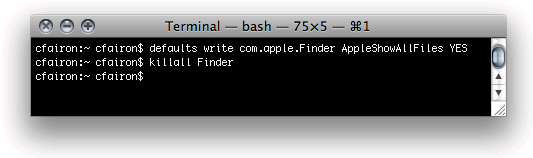
\includegraphics[width=12cm]{resources/img/fig-mac6.png}
\caption{Redémarrez le Finder\label{fig-mac6}}
\end{center}
\end{figure}

\bigskip
\noindent Pour revenir à la configuration d'origine, tapez: 

\bigskip
\verb+defaults write com.apple.Finder AppleShowAllFiles OFF+


\section{Première utilisation}
Si vous travaillez sous Windows, le programme vous demandera de choisir un répertoire personnel de travail
\index{Répertoire!personnel de travail}, que vous pourrez changer ultérieurement dans
"Info>Preferences...>Di-rectories". Pour créer un répertoire, cliquez sur l’icône représentant un
dossier (voir figure \ref{fig-creation-personal-directory}).

\bigskip
\noindent Sous Linux et MacOS, le programme créera automatiquement un répertoire personnel de travail,
appelé \verb+/unitex+, dans votre répertoire \verb+$HOME+. 

\bigskip
\noindent Le répertoire personnel de travail, ou répertoire de l'utilisateur, vous permettra de stocker vos
données Unitex personnelles. Pour chaque langue que vous utiliserez, le
programme copiera l’arborescence de la langue dans votre répertoire de travail,
à l’exception des dictionnaires. Vous pourrez ainsi modifier à votre guise votre copie des données
sans risquer d’endommager les données du système, stockées dans le
répertoire système Unitex.\index{Répertoire!système Unitex}


\begin{figure}[h]
\begin{center}
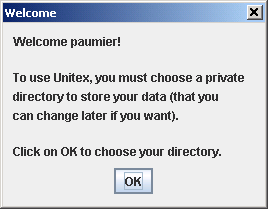
\includegraphics[width=6.3cm]{resources/img/fig1-1.png}
\caption{Première utilisation sous Windows}
\end{center}
\end{figure}

\begin{figure}[h]
\begin{center}
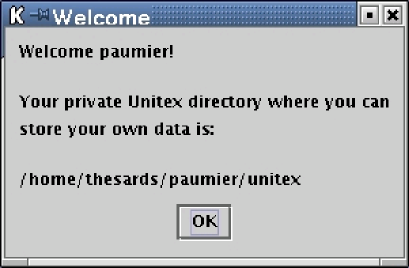
\includegraphics[width=7cm]{resources/img/fig1-2.png}
\caption{Première utilisation sous Linux}
\end{center}
\end{figure}

\begin{figure}[h]
\begin{center}
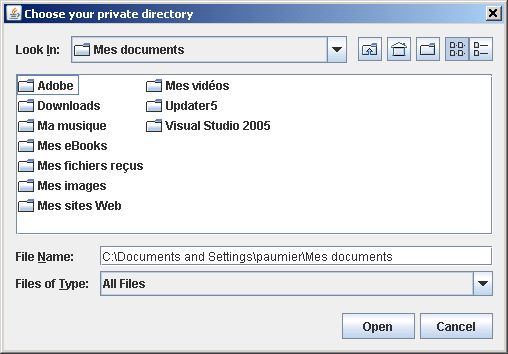
\includegraphics[width=13cm]{resources/img/fig1-3.png}
\caption{Création du répertoire personnel de travail
\label{fig-creation-personal-directory}}
\end{center}
\end{figure}



\section{Ajout de nouvelles langues}
\index{Ajout de nouvelles langues}

\bigskip
\noindent Il y a deux manières d’ajouter des langues. Si vous désirez ajouter une nouvelle langue
accessible à tous les utilisateurs, il vous faut copier le répertoire correspondant à cette langue
dans le répertoire système Unitex,\index{Répertoire!système Unitex}
ce qui nécessite d’avoir les droits d’accès à ce répertoire
(il vous faudra peut-être demander à votre administrateur système de le faire).
En revanche, si vous êtes le seul utilisateur concerné par la langue, vous pouvez copier le répertoire
en question dans votre répertoire de travail.\index{Répertoire!personnel de travail}
Vous pourrez ainsi travailler sur cette langue sans qu’elle soit proposée aux autres utilisateurs.



\section{Désinstallation}
Quel que soit le système sous lequel vous travaillez, il vous suffit de supprimer le répertoire
\verb+Unitex+ pour effacer tous les fichiers du système. Sous Windows, vous devrez ensuite supprimer
le raccourci vers \verb+Unitex.jar+ \index{Fichier!\verb+Unitex.jar+} si vous en avez créé un ;
même chose sous Linux ou MacOS si vous avez créé un alias.


\section{Unitex pour les développeurs}
\label{section-unitex-developpers}
Si vous êtes programmeur, cela peut vous intéresser de lier votre code avec les sources C++
d'Unitex. Pour faciliter cette opération, vous pouvez compiler Unitex en tant que librairie
dynamique qui contient toutes les fonctions Unitex functions, sauf \verb+main+s, bien sûr. La
page \url{http://docs.unitexgramlab.org/projects/unitex-library/fr/latest/} contient une documentation sur la librairie.


\bigskip
Sous Linux/MacOS, tapez:

\bigskip
\verb+make LIBRARY=yes+

\bigskip
\noindent et vous obtiendrez une librairie nommée \verb+libunitex.so+. Si vous souhaitez produire 
DLL Windows nommée \verb+unitex.dll+, utilisez les commandes suivantes:

\bigskip
Windows: \verb+make SYSTEM=windows LIBRARY=yes+

Cross-compilation avec mingw32: \verb+make SYSTEM=mingw32 LIBRARY=yes+

\bigskip
\noindent dans tous les cas, vous obtiendrez aussi un programme nommé
\verb+Test_lib+(\verb+.exe+). Si tout a bien fonctionné, ce programme devrait afficher l'écran
suivant:

\begin{verbatim}
Expression converted.
Reg2Grf exit code: 0

#Unigraph
SIZE 1313 950
FONT Times New Roman:  12
OFONT Times New Roman:B 12
BCOLOR 16777215
FCOLOR 0
ACOLOR 12632256
SCOLOR 16711680
CCOLOR 255
DBOXES y
DFRAME y
DDATE y
DFILE y
DDIR y
DRIG n
DRST n
FITS 100
PORIENT L
#
7
"<E>" 100 100 1 5
"" 100 100 0
"a" 100 100 1 6
"b" 100 100 1 4
"c" 100 100 1 6
"<E>" 100 100 2 2 3
"<E>" 100 100 1 1
\end{verbatim}

\chapter{Chargement d’un texte}
\label{chap-text}

\noindent Une des principales fonctionnalités d’Unitex est la recherche d’expressions dans des
textes. Pour cela, les textes doivent subir plusieurs opérations de prétraitement telles que
la normalisation de formes non ambiguës et le découpage du texte en phrases. Une fois
ces opérations effectuées, des dictionnaires électroniques sont appliqués aux textes. On peut
alors effectuer des recherches sur ces textes en leur appliquant des grammaires.


\bigskip
\noindent Ce chapitre décrit les différentes étapes du prétraitement des textes.


\section{Sélection de la langue}
\index{Sélection de la langue}
\noindent Lors du lancement d’Unitex, le programme vous demande de choisir la langue dans laquelle
vous allez travailler (voir figure~\ref{fig-language-selection}). Les langues proposées sont celles
qui sont présentes dans le répertoire système \verb+Unitex+ ainsi que celles éventuellement
installées dans votre répertoire personnel. Si vous utilisez une langue pour la première fois,
Unitex recopie le répertoire système de cette langue dans votre répertoire personnel, à l’exception
des  dictionnaires, afin d’économiser de l’espace disque.


\bigskip
\noindent Attention, si vous avez déjà un répertoire utilisateur pour une langue donnée, Unitex
n’essaiera pas de recopier les données système dedans. Ainsi, si une mise à jour a modifié un
fichier de ressource autre qu’un dictionnaire, il vous faudra soit faire une mise à jour manuelle
du fichier dans votre répertoire utilisateur, soit supprimer votre répertoire pour la langue
concernée et laisser à Unitex le soin de le recréer.


\bigskip
\noindent 
Le choix de la langue permet d’indiquer à Unitex où trouver certaines données, comme par exemple le
fichier alphabet. \index{Fichier!alphabet} Vous pouvez à tout moment changer de langue en cliquant
sur "Change Language..." dans le menu "Text". Si vous changez de langue, le programme fermera,
s’il y en a, toutes les fenêtres relatives au texte courant. La langue courante est indiquée sur
la barre de titre de l’interface graphique.


\begin{figure}[!h]
\begin{center}
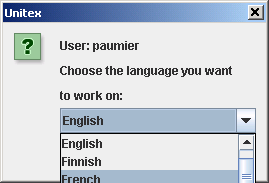
\includegraphics[width=6.2cm]{resources/img/fig2-1.png}
\caption{\label{fig-language-selection}Sélection de la langue au lancement d’Unitex}
\end{center}
\end{figure}


\section{Format des textes}
\label{section-conversion-texte-unicode}
\index{Format!des textes}
\index{Corpus|see{Texte}}
\index{Unicode}
Unitex manipule des textes Unicode. Unicode est un standard qui décrit un codage universel 
des caractères. Chaque caractère se voit attribuer un numéro unique, ce qui permet
de représenter des textes sans avoir à tenir compte des codages propres aux différentes 
machines et/ou systèmes d’exploitation. Unitex utilise une représentation codée sur deux 
octets du standard Unicode 3.0, appelée Unicode Little-Endian (pour plus de détails, voir
\cite{UNICODE}).

\bigskip
\index{Fichier!transcodage}
\noindent Les textes fournis avec Unitex sont déjà au format Unicode. Si vous essayez d’ouvrir un
texte qui n’est pas au format Unicode, le programme vous proposera de le convertir automatiquement 
(voir figure~\ref{auto-transcoding}). Cette conversion se base sur la langue courante : si vous
travaillez en français, Unitex vous proposera de convertir votre texte\footnote{Unitex propose
également de convertir automatiquement les graphes et dictionnaires qui ne sont pas en Unicode
Little-Endian.}, en supposant qu’il est codé avec un codage français. Par défaut, Unitex vous
propose soit de remplacer le texte original, soit de renommer le fichier d’origine en insérant
\verb$.old$ au début de son extension. Par exemple, si un fichier ASCII est nommé \verb$biniou.txt$,
le processus de conversion va créer une copie de ce fichier ASCII nommée \verb$biniou.old.txt$, et
va remplacer le contenu de \verb$biniou.txt$ par son équivalent en Unicode.

\begin{figure}[!h]
\begin{center}
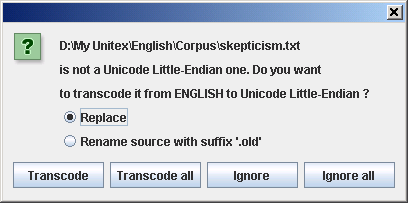
\includegraphics[width=10cm]{resources/img/fig2-2.png}
\caption{\label{auto-transcoding}Conversion automatique d’un texte non Unicode}
\end{center}
\end{figure}

\bigskip
\noindent Si le codage proposé par défaut n’est pas le bon, ou si vous voulez renommer le fichier
autrement qu’avec le suffixe \verb$.old$,vous pouvez utiliser la commande "Transcode Files"
dans le menu "File Edition". Cette commande vous permet de choisir les codages d’origine
et de destination des documents à convertir (voir figure~\ref{transcoding}). Par défaut, le codage
source proposé est celui qui correspond à la langue courante, et le codage de destination est
Unicode Little-Endian. Vous pouvez modifier ces choix, en sélectionnant n’importe quels
codages de source et destination. Ainsi, vous pouvez si vous le souhaitez convertir vos données
dans d’autres codages, comme par exemple UTF-8 si vous voulez en faire des pages
web. Le bouton "Add Files" vous permet de sélectionner les fichiers à convertir. Le bouton
"Remove Files" permet de retirer de la liste des fichiers sélectionnés par erreur. Le bouton
"Transcode" lancera la conversion de tous les fichiers. Si une erreur survient lors du traitement
d’un fichier (par exemple, un fichier qui serait déjà en Unicode), le traitement continue
avec le fichier suivant.


\begin{figure}[!h]
\begin{center}
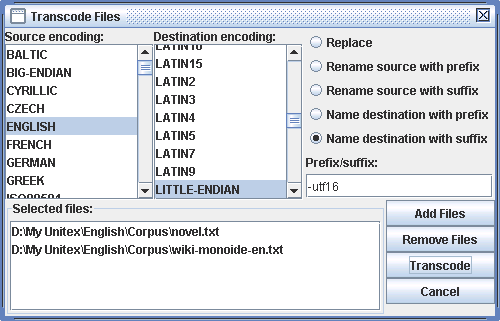
\includegraphics[width=12cm]{resources/img/fig2-3.png}
\caption{\label{transcoding}Conversion de fichiers}
\end{center}
\end{figure}

\noindent Pour obtenir du texte au bon format, vous pouvez également utiliser un traitement de
texte comme le logiciel libre OpenOffice.org (\cite{OpenOffice}) ou Microsoft Word, et sauvegarder
votre document au format "Texte unicode". Dans OpenOffice Writer, vous devez choisir le format
"Coded Text (*.txt)" puis le codage "Unicode" dans la fenêtre de configuration comme le montre la
figure~\ref{OfficeWriter}.

\begin{figure}[!h]
\begin{center}
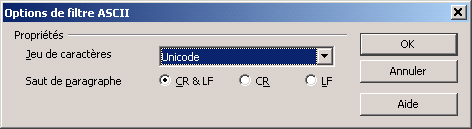
\includegraphics[width=12.5cm]{resources/img/fig2-4.png}
\caption{\label{OfficeWriter}Sauvegarde en Unicode dans OpenOffice Writer}
\end{center}
\end{figure}

\noindent Par défaut, le codage proposé sur un PC est toujours Unicode Little-Endian. Les textes 
ainsi obtenus ne contiennent plus d’informations de formatage (police, couleurs, etc.) et sont
prêts à être utilisés avec Unitex.

\bigskip
\noindent 
Vous pouvez choisir le codage par défaut, UTF16LE, UTF16BE ou UTF8 dans l'onglet, "Encoding" grâce
au sous-menu "Preference"  dans le menu "Info". Ce codage n'est valide que pour la langue
courante.

\begin{figure}[!h]
\begin{center}
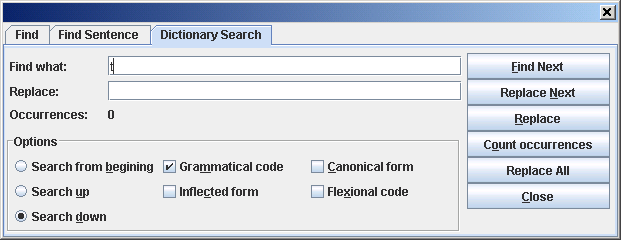
\includegraphics[width=10cm]{resources/img/fig2-5.png}
\caption{Choix de l'encodage par défaut pour la langue courante}
\end{center}
\end{figure}

% For small files...
\section{Édition de textes}
Vous avez également la possibilité d’utiliser l’éditeur de texte intégré à Unitex, accessible
via la commande "Open..." du menu "File Edition". Cet éditeur vous propose des fonctionnalités
de recherche et remplacement propres aux textes et dictionnaires manipulés par Unitex. Pour y
accéder, cliquez sur l’icône "Find" (jumelles). Vous verrez alors apparaître une fenêtre divisée en
trois onglets. L’onglet "Find" correspond aux opérations de recherche habituelles. Si vous ouvrez un
texte découpé en phrases, vous aurez la possibilité de faire une recherche par numéro de phrase dans
l’onglet "Find Sentence". Enfin, l’onglet "Dictionary Search", visible sur la
figure~\ref{dictionary-search}, vous permet d’effectuer des opérations propres aux dictionnaires
électroniques. En particulier, vous pouvez effectuer une recherche en spécifiant si elle doit porter
sur la forme fléchie, le lemme, les codes grammaticaux et sémantiques et/ou les codes flexionnels.
Ainsi, si vous voulez rechercher tous les verbes qui ont le trait sémantique
\verb$t$, marquant la transitivité, il vous suffit de chercher \verb$t$ en cochant
"Grammatical code". Vous obtiendrez ainsi les entrées voulues, sans ambiguïtés avec toutes les
autres occurrences de la lettre \verb$t$.


\begin{figure}[!h]
\begin{center}
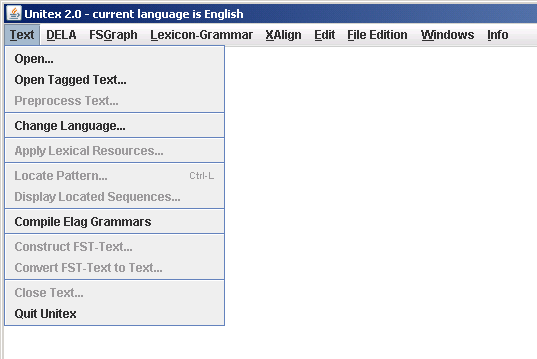
\includegraphics[width=15cm]{resources/img/fig2-6.png}
\caption{Recherche du trait sémantique \texttt{t}dans un dictionnaire
électronique\label{dictionary-search}}
\end{center}
\end{figure}


\section{Ouverture d’un texte}
\noindent Unitex propose d’ouvrir deux types de fichiers textes. \index{Fichier!texte}
Les fichiers portant l’extension \verb+.snt+ sont des fichiers textes prétraités 
par Unitex qui sont prêts à être manipulés par les différentes fonctions du système.
Les fichiers portant l’extension \verb+.txt+ sont des fichiers bruts.
Pour utiliser un texte, il faut donc commencer par ouvrir le fichier  \verb+.txt+
correspondant en cliquant sur "Open..." dans le menu "Text".


\begin{figure}[!h]
\begin{center}
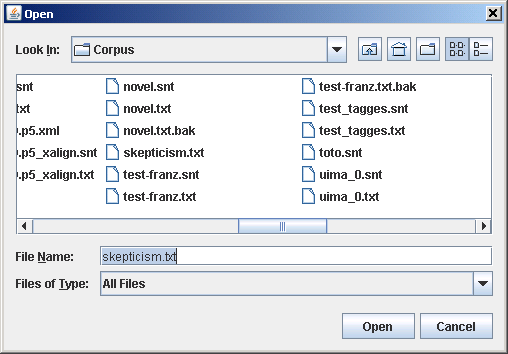
\includegraphics[width=14cm]{resources/img/fig2-7.png}
\caption{Menu Text}
\end{center}
\end{figure}

\begin{figure}[!h]
\begin{center}
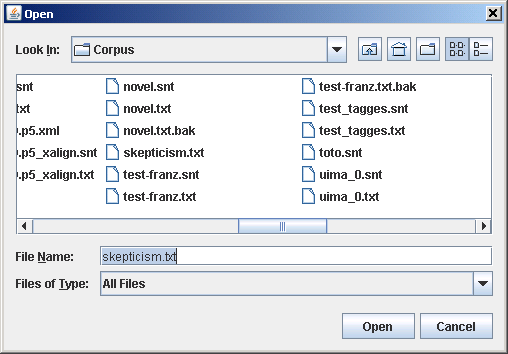
\includegraphics[width=13cm]{resources/img/fig2-8.png}
\caption{Ouverture d’un texte Unicode}
\end{center}
\end{figure}



\section{Prétraitement du texte}
\index{Texte!prétraitement}
\noindent Une fois le texte sélectionné, Unitex vous propose de le prétraiter. Le prétraitement du
texte consiste à lui appliquer les opérations suivantes : normalisation des séparateurs, 
découpage en unités lexicales, normalisation de formes non ambiguës, découpage en phrases
et application des dictionnaires. Si vous refusez le prétraitement, le texte sera néanmoins
normalisé et découpé en unités lexicales, car ces opérations sont indispensables au
fonctionnement d’Unitex. Il vous sera toujours possible d’effectuer le prétraitement plus tard,
en cliquant sur "Preprocess text..." dans le menu "Text".


\begin{figure}[!h]
\begin{center}
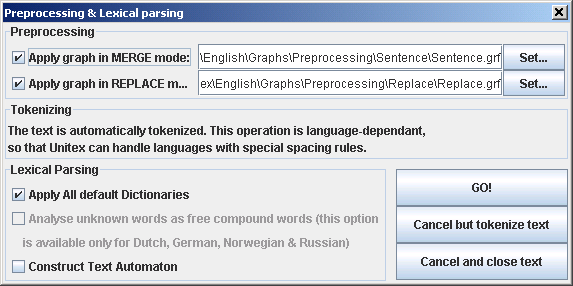
\includegraphics[width=15cm]{resources/img/fig2-9.png}
\caption{Fenêtre de prétraitement\label{fig-preprocessing-frame}}
\end{center}
\end{figure}

\bigskip
\noindent 
Si vous acceptez le prétraitement, Unitex vous proposera de le paramétrer grâce à la fenêtre de la
figure~\ref{fig-preprocessing-frame}. L’option "Apply FST2 in MERGE mode" sert à effectuer le
découpage du texte en phrases. L’option "Apply FST2 in REPLACE mode" est utilisée pour effectuer des
remplacements dans le texte, le plus souvent des normalisations de formes non ambiguës. L’option
"Apply All default Dictionaries" permet d’appliquer au texte des dictionnaires au format DELA
(Dictionnaires Electroniques du LADL). \index{DELA} L’option "Analyse unknown words as free 
compound words" est utilisée en norvégien pour analyser correctement les mots composés libres
formés par soudure de mots simples. Enfin, l’option "Construct Text Automaton" est utilisée
pour construire l’automate du texte. Cette option est désactivée par défaut, car elle entraîne
une forte consommation de mémoire et d’espace disque si le texte est trop volumineux. La
construction de l’automate du texte sera abordée dans le chapitre~\ref{chap-text-automaton}.

\bigskip
\noindent NOTE: si vous cliquez sur "Cancel but tokenize text", le programme effectuera malgré
tout la normalisation des séparateurs et le découpage en unités lexicales ; cliquez sur "Cancel
and close text" pour annuler complètement l’opération.


\subsection{Normalisation des séparateurs}
\index{Normalisation!des séparateurs}\index{Séparateurs de mots}\index{Texte!normalisation}
Les séparateurs usuels sont l’espace, la tabulation et le retour à la ligne. On peut rencontrer
plusieurs séparateurs consécutifs dans des textes, mais comme cela n’est d’aucune utilité
pour une analyse linguistique, on normalise ces séparateurs selon les règles suivantes:

\begin{itemize}
  \item toute suite de séparateurs contenant au moins un retour à la ligne est remplacée par
  un unique retour à la ligne
  \item toute autre suite de séparateurs est remplacée par un espace.
\end{itemize}

\bigskip
\noindent 
La distinction entre espace et retour à la ligne est conservée à cette étape car la présence
de retours à la ligne peut intervenir dans le découpage du texte en phrases. Le résultat de
la normalisation d’un fichier appelé \verb+mon_texte.txt+ est un fichier situé dans le même
répertoire que le \verb+.txt+ et dont le nom est \verb+mon_texte.snt+. \index{Fichier!\verb+.snt+}

\bigskip
\noindent NOTE: lorsque l’on prétraite un texte depuis l’interface graphique, un répertoire nommé

% do not remove this line jump 
\noindent \verb+mon_texte.snt+ est créé immédiatement après la normalisation. Ce répertoire, appelé
répertoire du texte, \index{Répertoire!du texte}
\index{Texte!répertoire du} contiendra toutes les données relatives à ce texte.



\subsection{Découpage en phrases}
\label{section-sentence-splitting}
\index{Découpage!en phrases}\index{Texte!découpage en phrases}
\index{Grammaires!découpage en phrases}
Le découpage en phrases est une étape importante du prétraitement car elle va permettre
de définir des unités de traitement linguistique. Ce découpage sera utilisé par le programme
de construction de l’automate du texte. Contrairement à ce que l’on pourrait penser, la re-
cherche des limites de phrases n’est pas un problème trivial. Considérons le texte suivant :


\bigskip
\textit{La famille a appelé le Dr. Martin en urgence.}

\bigskip \noindent Le point qui suit \textit{Dr} est suivi d’un mot commençant par une majuscule;
il pourrait donc être considéré comme un point de fin de phrase, ce qui serait faux. Afin d’éviter
les problèmes de ce genre, dus à des ambiguïtés des symboles de ponctuation, on utilise des
grammaires qui décrivent les différents contextes où peuvent apparaître les limites de phrases.
La figure~\ref{fig-example-sentence-splitting} montre un exemple de grammaire de découpage en
phrases.

\bigskip
\noindent  Lorsqu’un chemin de la grammaire reconnaît une séquence dans le texte et que ce chemin
produit le symbole délimiteur de phrases \verb+{S}+\index{\verb+{S}+}\index{Délimiteur de phrases},
on insère ce symbole dans le texte.

\bigskip
\noindent Ainsi,
un chemin de la grammaire de la figure~\ref{fig-example-sentence-splitting} reconnaît la séquence
composée d’un point d’interrogation et d’un mot commençant par une majuscule et insère le symbole 
\verb+{S}+ entre le point d’interrogation et le mot suivant. Le texte suivant :


\bigskip
\textit{Quelle heure est-il ? Huit heures.}

\bigskip
\noindent deviendrait donc :

\bigskip
\textit{Quelle heure est-il ?\{S\} Huit heures.}

\bigskip
\noindent Une grammaire de découpage peut manipuler les symboles spéciaux, ou méta-symboles, suivants :

\index{\verb+<E>+}\index{Epsilon|see{<E>}}
\index{\verb+<MOT>+}\index{\verb+<MIN>+}\index{\verb+<MAJ>+}\index{\verb+<PRE>+}\index{\verb+<NB>+}
\index{\verb+<PNC>+}\index{\verb+<^>+}\index{\verb+#+}\index{Méta-symboles}
\begin{itemize}
  \item <E> : mot vide, ou epsilon. Reconnaît la séquence vide;
  \item <MOT> : reconnaît n’importe quelle suite de lettres;
  \item <MIN> : reconnaît n’importe quelle suite de lettres minuscules;
  \item <MAJ> : reconnaît n’importe quelle suite de lettres majuscules;
  \item <PRE> : reconnaît n’importe quelle suite de lettres commençant par une majuscule;
  \item <NB> : reconnaît n’importe quelle suite de chiffres contigus (1234 est reconnu mais pas 1 234); 
  \item <PNC> : reconnaît les symboles de ponctuation ; , ! ? : ainsi que les points d’exclamation
  	  et d’interrogation inversés de l’espagnol et quelques signes de ponctuation asiatiques;
  \item <\verb+^+> : reconnaît un retour à la ligne;
  \item \verb+#+ : interdit la présence de l’espace.
\end{itemize}

\begin{figure}[!h]
\begin{center}
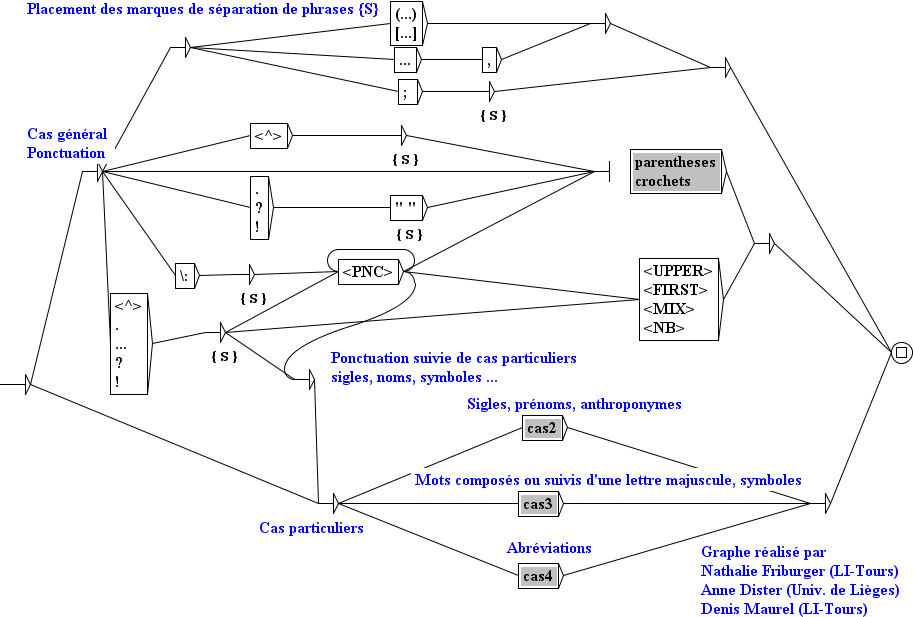
\includegraphics[width=15cm]{resources/img/fig2-10.png}
\caption{Grammaire de découpage en phrases pour le français
\label{fig-example-sentence-splitting}}
\end{center}
\end{figure}

\bigskip
\noindent Par défaut, l’espace est facultatif entre deux boîtes. Si l’on veut interdire la présence
de ce séparateur, il faut utiliser le symbole spécial \verb+#+. À l’inverse, si vous souhaitez
forcer la présence de l’espace, vous devez utiliser la séquence \verb+" "+. Les lettres minuscules
et majuscules sont définies par un fichier alphabet\index{Fichier!alphabet}\index{Alphabet}
(voir chapitre~\ref{chap-file-formats}). Pour plus de détails sur les graphes,
voir le chapitre~\ref{chap-grammars}. Pour plus de détails sur le découpage d’un texte en phrases,
voir \cite{ameliorer-decoupage-en-phrases}. La grammaire utilisée se nomme \verb+Sentence.fst2+ et
se trouve dans le répertoire suivant:\index{Fichier!\verb+Sentence.fst2+}

\bigskip
\verb+/(répertoire personnel)/(langue)/Graphs/Preprocessing/Sentence+

\bigskip
\noindent L’application de cette grammaire à un texte s’effectue grâce au programme \verb+Fst2Txt+
\index{\verb+Fst2Txt+}\index{Programmes externes!\verb+Fst2Txt+} en mode MERGE.\index{MERGE} 
Cela signifie que les sorties produites par la grammaire, en l’occurrence le symbole \verb+{S}+,
sont insérées dans le texte. Ce programme prend en entrée un fichier \verb+.snt+ et le modifie.


\subsection{Normalisation de formes non ambiguës}
\index{Normalisation!de formes non ambiguës}
\index{Grammaires!normalisation!de formes non ambiguës}

Certaines formes présentes dans les textes peuvent être normalisées (par exemple, la séquence
française "\textit{l'on}" est équivalente à la forme "\textit{on}"). Chaque utilisateur peut donc
vouloir effectuer des remplacements en fonction de ses besoins. Toutefois, il faut faire
attention à ce que les formes normalisées soient non ambiguës, ou à ce que la disparition de
l’ambiguïté soit sans conséquence pour l’application recherchée.


\bigskip
\noindent Si l’on décide de remplacer la forme "\textit{audit}" par "\textit{à le-dit}",
 la phrase :

\bigskip
\textit{La cour a procédé à un audit des comptes de cette société.}

\bigskip
\noindent sera remplacée par la phrase incorrecte :

\bigskip
\textit{La cour a procédé à un à le-dit des comptes de cette société.}

\bigskip
\noindent Il faut donc être très prudent lorsque l’on manipule la grammaire de normalisation.
Il faut également faire attention aux espaces.
En effet, si l’on remplace "\textit{c’}" par "\textit{ce}" non suivi par un espace, la phrase :


\bigskip
\textit{Est-ce que c’était toi ?}

\bigskip
\noindent sera remplacée par la séquence incorrecte :

\bigskip
\textit{Est-ce que ce était toi ?}

%\bigskip
%\noindent To avoid this problem, one should explicitly insert a space,
%\textit{i.e.} replace "\textit{'re}" by "\textit{ are}".

\bigskip
\noindent Les symboles acceptés par les grammaires de normalisation sont les mêmes que ceux
autorisés dans les grammaires de découpage en phrases. La grammaire utilisée se nomme
\verb+Replace.fst2+ et se trouve dans le répertoire suivant :

\bigskip \verb+/(répertoire personnel)/(langue)/Graphs/Preprocessing/Replace+

\bigskip
\noindent Comme pour le découpage en phrases, cette grammaire est utilisée avec le programme
\verb+Fst2Txt+ \index{Programmes externes!\verb+Fst2Txt+}\index{\verb+Fst2Txt+}, mais cette fois en
mode REPLACE, ce qui signifie que les entrées reconnues par la grammaire sont remplacées par les
séquences produites par celle-ci. On peut voir sur la figure~\ref{fig-normalization-grammar} une
grammaire qui normalise des contractions verbales en anglais.

\begin{figure}[!p]
\begin{center}
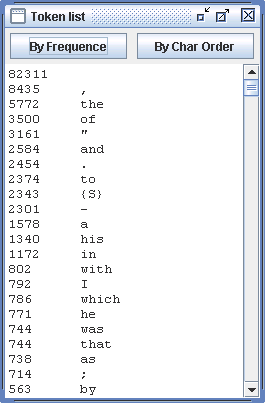
\includegraphics[width=14cm]{resources/img/fig2-11.png}
\caption{Grammaire de normalisation de formes verbales en anglais\label{fig-normalization-grammar}}
\end{center}
\end{figure}



\subsection{Découpage du texte en unités lexicales}
\index{Texte!découpage en unités lexicales}
\index{Découpage!en unités lexicales}
\index{Token}\index{Tokenisation}
\label{tokenization}
Certaines langues, en particulier les langues asiatiques, utilisent les séparateurs de façon
différente des langues occidentales ; les espaces peuvent être interdits, facultatifs ou
obligatoires. Pour pouvoir gérer ces particularités au mieux, Unitex découpe les textes d’une
manière dépendante de la langue. Ainsi, les langues comme le français sont traitées selon le
principe suivant :

\bigskip
\noindent Une unité lexicale peut être :
\begin{itemize}
  \item soit le délimiteur de phrases \verb+{S}+;
  \item le marqueur \verb+{STOP}+.\index{\verb${STOP}$} Contrairement au délimiteur de phrases
  \verb+{S}+, le marqueur \verb+{STOP}+ ne peut JAMAIS être reconnu par une grammaire, de quelque
  façon que ce soit. Il peut être utilisé dans un corpus pour délimiter des élements. Par exemple,
  si un corpus est formé de nouvelles séparées par \verb+{STOP}+, il est impossible pour une
  grammaire de reconnaître une séquence qui chevauche la fin d'une nouvelle et le début de la
  suivante;
  \item une étiquette lexicale \verb+{aujourd'hui,.ADV}+;
  \item une séquence de lettres contiguës (les lettres sont définies dans le fichier alphabet de la
  langue);
  \index{Fichier!alphabet}
  \item un (et un seul) caractère différrent d'une lettre, i.e. tous les caractères non définis
  dans le fichier alphabet de la langue courante; s'il s'agit d'une newline, il est remplacé par un
  espace.
\end{itemize}

\bigskip
\noindent Pour les autres langues, le découpage est effectué caractère par caractère, à l’exception
du délimiteur de phrases \verb+{S}+ le marqueur \verb+{STOP}+ et des étiquettes lexicales. Ce
découpage basique garantit le fonctionnement d’Unitex, mais limite l’optimisation des opérations de
recherche de motifs.


\bigskip
\noindent Quel que soit le mode de découpage, les retours à la ligne présents
dans un texte sont remplacés par des espaces. Ce découpage est effectué par le programme
\verb+Tokenize+\index{\verb+Tokenize+} \index{Programmes externes!\verb+Tokenize+}.
Ce programme produit plusieurs fichiers, stockés dans le répertoire du texte :
\begin{itemize}
  \item \verb+tokens.txt+ contient la liste des unités lexicales dans l’ordre où elles ont été
  	  trouvées dans le texte;\index{Fichier!\verb+tokens.txt+}
  \item \verb+text.cod+  contient un tableau d’entiers; chaque entier correspondant à l’indice d’une
  	  unité lexicale dans le fichier \verb+tokens.txt+;
  \index{Fichier!\verb+text.cod+}
  \item \verb+tok_by_freq.txt+ contient la liste des unités lexicales triée par ordre de fréquence;
  \index{Fichier!\verb+tok_by_freq.txt+}
  \item \verb+tok_by_alph.txt+ contient la liste des unités lexicales triée par ordre alphabétique;
  \index{Fichier!\verb+tok_by_alph.txt+}
\item \verb+stats.n+ contient quelques statistiques sur le texte. \index{Fichier!\verb+stats.n+}
\end{itemize}

\bigskip
\noindent Le découpage du texte :

\bigskip
\textit{Un sou c’est un sou.}

\bigskip
\noindent donne la liste d’unités lexicales suivantes :  \textit{UN} ESPACE \textit{sou c ’ est un
.}

\bigskip
\noindent On peut remarquer qu’il est tenu compte de la casse (Un et un sont deux unités distinctes), mais que chaque unité n’est codée qu’une fois. En numérotant ces unités de 0 à 7,
ce texte peut être représenté par la séquence d’entiers décrite dans le tableau suivant :

\bigskip
\begin{table}[h]
\begin{center}
\begin{tabular}{|p{2.8cm}||c|c|c|c|c|c|c|c|c|c|c|c|}
\hline
Indice             & 0 & 1 & 2 & 1 & 3 & 1 & 4 & 1 & 2 & 5
\\
\hline
Unité lexicale correspondante & \textit{UN} &   & \textit{sou} &   & \textit{est} &  & \textit{UN}
& & \textit{sou} & \textit{.}
\\
\hline
\end{tabular}
\caption{Représentation du texte \textit{Un sou c’est un sou.}}
\end{center}
\end{table}

\bigskip
\noindent Pour plus de détails, voir le chapitre~\ref{chap-file-formats}.

\begin{figure}[!h]
\begin{center}
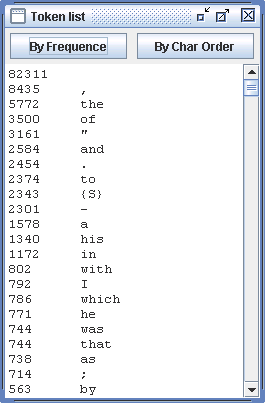
\includegraphics[height=10cm]{resources/img/fig2-12.png}
\caption{Unités lexicales d’un texte anglais triées par fréquence}
\end{center}
\end{figure}



\subsection{Application de dictionnaires}
\label{text-applying-dictionaries}
\index{Dictionnaire!application}
\index{Ressources!lexicales|see{Dictionnaire}}
L’application de dictionnaires consiste à construire le sous-ensemble des dictionnaires
ne contenant que les formes présentes dans le texte. Ainsi, le résultat de l’application des
dictionnaires du français au texte \textit{Igor mange une pomme de terre} produit le dictionnaire de
mots simples suivant :
\index{Mots!simples}

\bigskip
\begin{verbatim}
de,.DET+z1
de,.PREP+z1
de,.XI+z1
mange,manger.V+z1:P1s:P3s:S1s:S3s:Y2s
pomme,.A+z1:ms:fs:mp:fp
pomme,.N+z1:fs
pomme,pommer.V+z3:P1s:P3s:S1s:S3s:Y2s
terre,.N+z1:fs
terre,terrer.V+z1:P1s:P3s:S1s:S3s:Y2s
une,.N+z1:fs
une,un.DET+z1:fs
\end{verbatim}

\bigskip
\noindent ainsi que le dictionnaire de mots composés contenant l’unique entrée
:\index{Mots!composés}

\bigskip
\begin{verbatim}
pomme de terre,.N+z1:fs
\end{verbatim}

\bigskip
\noindent La séquence \textit{Igor} n'étant ni un mot simple du français, ni une partie de mot
composé, a été considérée comme un mot inconnu.\index{Mots!inconnus} L’application de dictionnaires
s’effectue avec le programme \verb+Dico+.\index{\verb+Dico+}\index{Programmes externes!\verb+Dico+}
Les trois fichiers produits (\verb+dlf+ pour les mots simples, \verb+dlc+ pour les mots composés et
\verb+err+ pour les mots inconnus) sont placés dans le répertoire du texte. On appelle dictionnaires
du texte les fichiers \verb+dlf+ et \verb+dlc+
\index{Dictionnaire!du texte}
\index{Fichier!\verb+dlf+}
\index{Fichier!\verb+dlc+}\index{Fichier!\verb+err+}

\bigskip
\noindent Une fois l’application des dictionnaires effectuée, Unitex présente par ordre alphabétique
les mots simples, composés et inconnus trouvés dans une fenêtre. La figure~\ref{fig-Dico-application-results} montre les résultats pour un texte anglais.

\begin{figure}[!ht]
\begin{center}
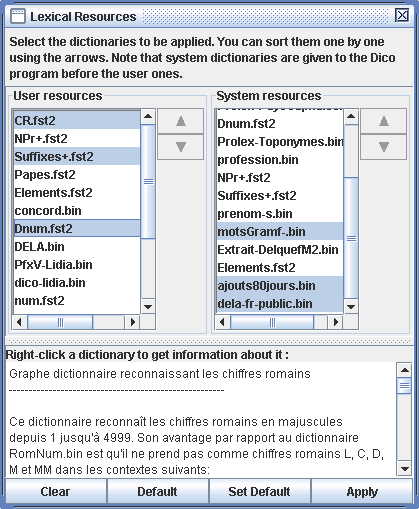
\includegraphics[width=12cm]{resources/img/fig2-13.png}
\caption{Résultats de l’application de dictionnaires sur un texte
anglais\label{fig-Dico-application-results}}
\end{center}
\end{figure}

\bigskip
\noindent Il est également possible d’appliquer des dictionnaires en dehors du prétraitement du
texte. Pour cela, il faut cliquer sur "Apply Lexical Resources..." dans le menu "Text". Unitex
affiche alors une fenêtre (voir figure ~\ref{fig-Dico-configuration}) qui permet de choisir la
liste des dictionnaires à appliquer.


\begin{figure}[!ht]
\begin{center}
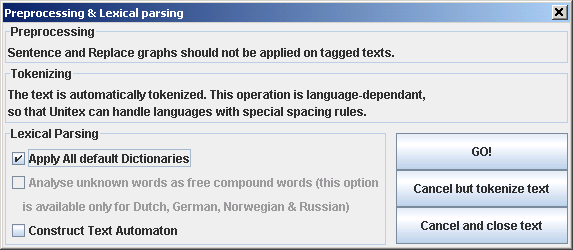
\includegraphics[width=10cm]{resources/img/fig2-14.png}
\caption{Paramétrage de l’application des dictionnaires\label{fig-Dico-configuration}}
\end{center}
\end{figure}

\bigskip
\noindent La liste "User resources" recense tous les dictionnaires \verb+.bin+ et \verb+.fst2+
présents dans le répertoire \verb+(langue)/Dela+ de l’utilisateur. Les dictionnaires du système sont
listés dans le cadre intitulé "System resources". Utilisez <Ctrl+click> pour sélectionner plusieurs
dictionnaires. Les dictionnaires systèmes sont appliqués avant les dictionnaires utilisateurs.
Vous pouvez choisir l'ordre des dictionnaires des listes utililisateur et système à l'aide des
flèches haut et bas (voir figure \ref{fig-Dico-configuration}). Le bouton "Set Default" vous permet
de définir la sélection courante de dictionnaires comme sélection par défaut. Cette sélection par
défaut sera utilisée lors du prétraitement si vous choisissez l’option "Apply All default
Dictionaries".\index{Dictionnaire!sélection par défaut}
Si vous effectuez un clic droit au-dessus d’un nom de dictionnaire, la documentation du
dictionnaire, si elle existe, s’affichera dans le cadre inférieur.


\subsection{Analyse des mots composés libres en néerlandais, allemand, norvégien et russe}
\index{Norvégien!mots composés libres}
\index{Allemand!mots composés libres}
\index{Néerlandais!mots composés libres}
\index{Russe!mots composés libres}
\index{Analyse des mots composés libres!langues germaniques}
\index{Mots!composés libres!langues germaniques}
\index{Analyse des mots composés libres!russe}
\index{Mots!composés libres!russe}

\label{section-Norwegian-compound-words}
Dans certaines langues comme le norvégien, il est possible de former des mots composés
libres en soudant leurs éléments. Par exemple, le mot \textit{aftenblad} signifiant \textit{journal
du soir} est obtenu en combinant les mots \textit{aften} (\textit{soir}) et \textit{blad}
(\textit{journal}). Le programme \verb+PolyLex+ \index{\verb+PolyLex+}\index{Programmes
externes!\verb+PolyLex+} explore la liste des mots inconnus après application des dictionnaires au
texte et essaye d’analyser chacun de ces mots comme un mot composé. Si un mot possède au moins une
analyse, il est retiré de la liste des mots inconnus et les lignes de dictionnaires produites pour
ce mot sont ajoutées au dictionnaire des mots simples du texte.

\section{Ouverture d’un texte taggué}
Un texte taggué est un texte contenant des entrées lexicales entre accolades comme par
exemple :


\bigskip
\textit{I do not like the \{square bracket,.N\} sign! \{S\}}

\bigskip
\noindent De tels tags permettent de lever des ambiguïtés en interdisant tout autre interprétation.
Dans notre exemple, on ne pourra pas reconnaître square bracket comme combinaison de deux mots
simples.


\bigskip
\noindent Toutefois, la présence de ces tags peut perturber l’application des graphes de
prétraitement. L’utilisateur dispose donc de la commande "Open Tagged Text..." dans le menu "Text",
grâce à laquelle il peut ouvrir un texte contenant des tags sans que les graphes de prétraitements
ne soient appliqués, comme on le voit sur la figure \ref{preprocess-tagged-text}.

\bigskip
\begin{figure}[!h]
\begin{center}
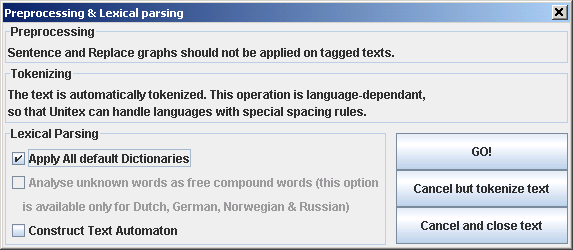
\includegraphics[width=14cm]{resources/img/fig2-15.png}
\caption{Prétraitement d’un texte taggué\label{preprocess-tagged-text}}
\end{center}
\end{figure}


\chapter{Dictionnaires}
\label{chap-dictionaries}

\section{Les dictionnaires DELA}
\index{DELA}\index{Dictionnaires!format}\index{LADL}

Les dictionnaires électroniques utilisés par Unitex utilisent le formalisme DELA (Dictionnaires
Electroniques du LADL). Ce formalisme permet de décrire les entrées lexicales simples et composées
\index{Entrées!lexicales} d’une langue en leur associant de façon optionnelle des
informations grammaticales, sémantiques et flexionnelles. On distingue deux sortes de dictionnaires
électroniques. Le type que l’on utilise le plus couramment est le dictionnaire de formes fléchies,
appelé DELAF (DELA de formes Fléchies) ou encore DELACF (DELA de formes Composées
Fléchies) lorsqu’il s’agit d’un dictionnaire de mots composés.\index{DELAF|(}
\index{DELACF}\index{Dictionnaires!DELAF|(}\index{Dictionnaires!DELACF}
Le second type est le dictionnaire de formes non fléchies appelé DELAS (DELA de formes Simples)
ou DELAC (DELA de formes Composées).
\index{DELAS}\index{DELAC}\index{Dictionnaires!DELAS}\index{Dictionnaires!DELAC}
Les programmes d’Unitex ne font pas de distinction entre les dictionnaires de formes
simples et composées. Nous utiliserons donc les termes DELAF et DELAS pour désigner les deux sortes
de dictionnaires que leurs entrées soient simples, composées ou mixtes.

\subsection{Format des DELAF}
\label{section-DELAF-format}
\subsubsection{Syntaxe d’une entrée}
Une entrée d’un DELAF est une ligne de texte terminée par un retour à la ligne qui
respecte le schéma suivant :

\bigskip
\begin{verbatim}
mercantiles,mercantile.A+z1:mp:fp/ceci est un exemple
\end{verbatim}

\bigskip
\noindent Les différents éléments qui forment cette ligne sont les suivants:

\bigskip
\begin{itemize}
\item \verb+mercantiles + est la forme fléchie de l’entrée.\index{Forme!fléchie} Cette forme fléchie
est obligatoire;
  
\bigskip \item \verb+mercantile+ est la forme canonique (lemme) de l’entrée.
\index{Lemme}\index{Forme!canonique} Pour les noms et les adjectifs, il s’agit
en général de la forme au masculin singulier; pour les verbes, la forme canonique est
l’infinitif. Cette information peut être omise comme dans l’exemple suivant :

  
\bigskip
\verb$boîte à merveilles,.N+z1:fs$
  
\bigskip Cela signifie alors que la forme canonique est identique à la forme fléchie. La forme
canonique est séparée de la forme fléchie par une virgule;
\index{\verb+,+}
  
\bigskip \item \verb$A+z1$ est la séquence d’informations grammaticales et sémantiques.
\index{Informations!grammaticales}\index{Informations!sémantiques} Dans notre exemple, \verb+A+
désigne un adjectif, et \verb+z1+ ndique qu’il s’agit d’un mot courant (voir tableau ~\ref{tab-semantic-codes}).

Toute entrée doit comporter au moins un code grammatical ou sémantique, séparé de
la forme canonique par un point. S’il y a plusieurs codes, ceux-ci doivent être séparés
par le caractère \verb$+$\index{\verb$+$}\index{\verb+.+}.
  
\bigskip
\item \verb+:mp:fp+ est la séquence d’informations flexionnelles.
\index{Informations!flexionnelles} Ces informations décrivent le genre, le nombre, les temps et modes
de conjugaisons, les déclinaisons pour les langues à cas, etc. Ces informations sont facultatives.
Un code flexionnel est composé d’un ou plusieurs caractères codant chacun une information. Les codes
flexionnels doivent être séparés par le caractère :. Dans notre exemple, \verb+m+ signifie masculin,
\verb+p+ pluriel et \verb+f+ féminin (voir tableau ~\ref{tab-inflectional-codes}). Le caractère \verb+:+ s’interprète comme un OU logique. Ainsi, \verb+:mp:fp+ signifie "masculin pluriel", ou "féminin pluriel". Comme chaque caractère correspond à une information, il est inutile d’utiliser plusieurs fois un même caractère. Ainsi, coder le participe passé avec le code\verb+:PP+ serait strictement équivalent à utiliser \verb+:P+ seul;\index{\verb+:+}
  
\bigskip \item \verb+/ceci est un exemple+ est un commentaire. Les commentaires sont facultatifs et
doivent être introduits par le caractère \verb+/+. Les commentaires sont supprimés lorsque
l’on comprime les dictionnaires. \index{Commentaire!dans un dictionnaire} \index{Dictionnaires!commentaire}\index{\verb+/+}
\end{itemize}

\bigskip
\noindent REMARQUE IMPORTANTE : il est possible d’utiliser le point et la virgule dans une
entrée de dictionnaire. Pour cela, il faut les déspécialiser avec le caractère
\verb+\+ \index{\verb+\,+}\index{\verb+\.+}\index{\verb+\+}:

\bigskip
\begin{verbatim}
3\,1415,PI.NOMBRE
Organisation des Nations Unies,O\.N\.U\..SIGLE
\end{verbatim}


\bigskip
\noindent ATTENTION : chaque caractère est pris en compte dans une ligne de dictionnaire. Par
exemple, si vous introduisez des espaces, ceux-ci seront considérés comme faisant partie
intégrante des informations. Dans la ligne suivante :


\begin{verbatim}
gît,gésir.V+z1:P3s /voir ci-gît
\end{verbatim}

\bigskip \noindent l’espace qui précède le caractère \verb+/+ sera considéré comme faisant partie
d’un code flexionnel à 4 caractères composés de \verb+P+, \verb+3+, \verb+s+ et d’un espace.


\bigskip \noindent Il est possible d’insérer des lignes de commentaires dans un dictionnaire DELAF
ou DELAS, en faisant débuter la ligne par le caractère $/$. Exemple

\bigskip
\begin{verbatim}
/ L’entrée nominale pour ’par’ est un terme de golf
par,.N+z3:ms
\end{verbatim}


\subsubsection{Mots composés avec espace ou tiret}

\index{Mots!composés!avec espace ou tiret}\index{\verb+=+}\index{\verb+\=+}

Certains mots composés comme \textit{grand-mère} peuvent s’écrire avec des espaces ou avec
des tirets. Pour éviter de devoir dédoubler toutes les entrées, il est possible d’utiliser 
le caractère \verb+=+ . Lors de la compression du dictionnaire, le programme \verb+Compress+
\index{Programmes externes!\verb+Compress+}\index{\verb+Compress+} vérifie pour chaque ligne
si la forme fléchie ou la forme canonique contient le caractère \verb+=+. Si c’est le cas, le
programme remplace l’entrée par deux entrées : une où le caractère = est remplacé par un espace,
et une où il est remplacé par un tiret. Ainsi, l’entrée suivante :


\bigskip \verb$grand=mères,grand=mère.N:fp$

\bigskip
\noindent est remplacée par les deux lignes suivantes:

\bigskip
\verb$grand mères,grand mère.N:fp$

\verb$grand-mères,grand-mère.N:fp$


\bigskip
\noindent NOTE : si vous souhaitez écrire une entrée contenant le caractère \verb+=+,
déspécialisez-le avec le caractère \verb+\+ comme dans l’exemple suivant :


\bigskip
\verb$E\=mc2,.FORMULE$\\


Cette opération de remplacement a lieu lors de la compression du dictionnaire. Une fois
le dictionnaire comprimé, les signes \verb+=+ déspécialisés sont remplacés par de simples \verb+=+.
Ainsi, si l’on comprime un dictionnaire contenant les lignes suivantes :


\begin{verbatim}
E=mc2,.FORMULE
grand=mère,.N:fs
\end{verbatim}

\noindent et que l’on applique ce dictionnaire au texte :\\

\verb$Ma grand-mère m’a expliqué la formule E=mc2.$


\bigskip \noindent on obtiendra les lignes suivantes dans le dictionnaire de mots composés du texte:


\begin{verbatim}
E=mc2,.FORMULE
grand-mère,.N:fs
\end{verbatim}


\subsubsection{Factorisation d’entrées}

Plusieurs entrées ayant les mêmes formes fléchie et canonique peuvent être regroupées
en une seule à condition qu’elle aient les mêmes codes grammaticaux et sémantiques. Cela
permet entre autres de regrouper des conjugaisons identiques pour un même verbe :


\bigskip
\begin{verbatim}
glace,glacer.V+z1:P1s:P3s:S1s:S3s:Y2s
\end{verbatim}

\bigskip 
\noindent Si les informations grammaticales et sémantiques diffèrent, il faut créer des entrées dis-
tinctes :


\bigskip
\begin{verbatim}
glace,.N+z1:fs
glace,glacer.V+z1:P1s:P3s:S1s:S3s:Y2s
\end{verbatim}

\bigskip 
\noindent Certaines entrées ayant les mêmes codes grammaticaux et sémantiques peuvent avoir
des sens différents, comme c’est le cas pour le mot \textit{poêle} qui désigne un appareil de
chauffage ou un voile au masculin et un instrument de cuisine au féminin. On peut donc distinguer
les entrées dans ce cas :


\bigskip
\noindent
\texttt{poêle,.N+z1:fs/ poêle à frire}

\noindent
\texttt{poêle,.N+z1:ms/ voile, linceul; appareil de chauffage}

\bigskip 
\noindent NOTE : dans la pratique, cette distinction n’a pas d’autre conséquence qu’une
augmentation du nombre d’entrées du dictionnaire. Les différents programmes qui composent Unitex
donneront exactement les mêmes résultats si l’on fusionne ces entrées en :

\bigskip
\noindent
\texttt{poêle,.N+z1:fs:ms}

\bigskip 
\noindent L’intérêt de cette distinction est donc laissé à l’appréciation des personnes qui
construisent des dictionnaires.


\index{DELAF|)}\index{Dictionnaires!DELAF|)}

\subsection{Format des DELAS}
\label{section-DELAS-format}
\index{DELAS}\index{Dictionnaires!DELAS}

Le format des DELAS est très similaire à celui des DELAF. La différence est qu’on ne
mentionne qu’une forme canonique suivie de codes grammaticaux et/ou sémantiques. La
forme canonique est séparée des différents codes par une virgule. Voici un exemple d’entrée :


\begin{verbatim}
cheval,N4+Anl
\end{verbatim}

\noindent Le premier code grammatical ou sémantique sera interprété par le programme de flexion
comme le nom de la grammaire à utiliser pour fléchir l’entrée. L’entrée de l’exemple cidessus
indique que le mot \textit{cheval} doit être fléchi avec une grammaire nommée \verb+N4+.
Il est possible d’ajouter des codes flexionnels aux entrées, mais la nature de l’opération de
flexion limite l’intérêt de cette possibilité. Pour plus de détails, voir plus loin dans ce chapitre
la section ~\ref{section-automatic-inflection}.


\subsection{Contenu des dictionnaires}
\index{Dictionnaires!contenus}\index{Dictionnaires!codes utilisés}

Les dictionnaires fournis avec Unitex contiennent des descriptions des mots simples et
composés. Ces descriptions indiquent la catégorie grammaticale de chaque entrée, ses 
éventuels codes de flexion, ainsi que des informations sémantiques diverses. Les tableaux 
suivants donnent un aperçu des différents codes utilisés dans les dictionnaires fournis avec
Unitex. Ces codes ont la même signification pour presque toutes les langues, même si certains
d’entre eux sont propres à certaines langues (\textit{i.e.} marque du neutre, etc.).

\begin{table}[!h]
\index{\verb+A+}\index{\verb+ADV+}\index{\verb+CONJC+}\index{\verb+CONJS+}\index{\verb+DET+}
\index{\verb+INTJ+}\index{\verb+N+}\index{\verb+PREP+}\index{\verb+PRO+}\index{\verb+V+}
\begin{center}
\begin{tabular}{|c|l|l|}
\hline
\textbf{Code} & \textbf{Signification} & \textbf{Exemples} \\
\hline
\verb+A+ & adjectif & fabuleux, broken-down \\
\hline
\verb+ADV+ & adverbe & réellement, à la longue \\
\hline
\verb+CONJC+ & conjonction de coordination & mais\\
\hline
\verb+CONJS+ & conjonction de subordination & puisque, à moins que \\
\hline
\verb+DET+ & déterminant & ses, trente-six \\
\hline
\verb+INTJ+ & interjection & adieu, mille millions de mille sabords \\
\hline
\verb+N+ & nom & prairie, vie sociale\\
\hline
\verb+PREP+ & préposition & sans, à la lumière de \\
\hline
\verb+PRO+ & pronom & tu, elle-même \\
\hline
\verb+V+ & verbe & continuer, copier-coller\\
\hline
\end{tabular}
\caption{Codes grammaticaux usuels\label{tab-grammatical-codes}}
\end{center}
\end{table}
\vspace{-0.7cm}
\begin{table}[!h]
\index{\verb+z1+}\index{\verb+z2+}\index{\verb+z3+}\index{\verb+Abst+}\index{\verb+Anl+}\index{\verb+AnlColl+}
\index{\verb+Conc+}\index{\verb+ConcColl+}\index{\verb+Hum+}\index{\verb+HumColl+}\index{\verb+t+}\index{\verb+i+}
\index{\verb+en+}\index{\verb+se+}\index{\verb+ne+}
\begin{center}
\begin{tabular}{|c|l|l|}
\hline
\textbf{Code} & \textbf{Signification} & \textbf{Exemple} \\
\hline
\verb+z1+ & langage courant & blague \\
\hline
\verb+z2+ & langage spécialisé & sépulcre \\
\hline
\verb+z3+ & langage très spécialisé & houer \\
\hline
\verb+Abst+ & abstrait & bon goût \\
\hline
\verb+Anl+ & animal & cheval de race \\
\hline
\verb+AnlColl+ & animal collectif & troupeau \\
\hline
\verb+Conc+ & concret & abbaye \\
\hline
\verb+ConcColl+ & concret collectif & décombres \\
\hline
\verb+Hum+ & humain & diplomate \\
\hline
\verb+HumColl+ & humain collectif & vieille garde \\
\hline
\verb+t+ & verbe transitif & foudroyer \\
\hline
\verb+i+ & verbe intransitif & fraterniser \\
\hline
\verb+en+ & particule pré-verbale (PPV) obligatoire & en imposer \\
\hline
\verb+se+ & verbe pronominal & se marier \\
\hline
\verb+ne+ & verbe à négation obligatoire & ne pas cesser de \\
\hline
\end{tabular}
\caption{Quelques codes sémantiques\label{tab-semantic-codes}}
\end{center}
\end{table}

%\bigskip
\noindent NOTE : les descriptions des temps du tableau ~\ref{tab-inflectional-codes} correspondent
au français. Néanmoins, la plupart de ces définitions se retrouvent dans plusieurs langues
(infinitif, présent, participe passé, etc.).


\bigskip
\noindent Malgré une base commune à la plupart des langues, les dictionnaires contiennent des
particularités de codage propres à chaque langue. Ainsi, les codes de flexion variant
beaucoup d’une langue à une autre, n’ont pas été décrits ici. Pour une description exhaustive
de tous les codes utilisés dans un dictionnaire, nous vous recommandons de vous adresser
directement à l’auteur du dictionnaire.


\begin{table}[!h]
\index{\verb+m+}\index{\verb+f+}\index{\verb+n+}\index{\verb+s+}\index{\verb+p+}\index{\verb+1+}
\index{\verb+2+}\index{\verb+3+}\index{\verb+P+}\index{\verb+I+}\index{\verb+S+}\index{\verb+T+}
\index{\verb+Y+}\index{\verb+C+}\index{\verb+J+}\index{\verb+W+}\index{\verb+G+}\index{\verb+K+}
\index{\verb+F+}
\begin{center}
\begin{tabular}{|c|l|}
\hline
\textbf{Code} & \textbf{Signification} \\
\hline
\verb+m+ & masculin \\
\hline
\verb+f+ & féminin \\
\hline
\verb+n+ & neutre \\
\hline
\verb+s+ & singulier \\
\hline
\verb+p+ & pluriel \\
\hline
\verb+1+, \verb+2+, \verb+3+ & 1st, 2nd, 3rd personne\\
\hline
\verb+P+ & présent de l’indicatif \\
\hline
\verb+I+ & imparfait de l’indicatif  \\
\hline
\verb+S+ & présent du subjonctif\\
\hline
\verb+T+ & imparfait du subjonctif \\
\hline
\verb+Y+ & présent de l’impératif \\
\hline
\verb+C+ & présent du conditionnel\\
\hline
\verb+J+ & passé simple \\
\hline
\verb+W+ & infinitif \\
\hline
\verb+G+ & participe présent \\
\hline
\verb+K+ & participe passé \\
\hline
\verb+F+ & futur \\
\hline
\end{tabular}
\caption{Codes flexionnels usuels\label{tab-inflectional-codes}}
\end{center}
\end{table}


\bigskip
\noindent Les codes présentés ne sont absolument pas limitatifs. Chaque utilisateur peut introduire
ses propres codes, et créer ses propres dictionnaires. Par exemple, on pourrait dans un but
pédagogique introduire dans les dictionnaires anglais des marques indiquant les faux-amis
français :

\bigskip
\begin{verbatim}
bless,.V+faux-ami/bénir
cask,.N+faux-ami/tonneau
journey,.N+faux-ami/voyage
\end{verbatim}

Il est également possible d’utiliser les dictionnaires pour stocker des informations parti-
culières. Ainsi, on pourrait utiliser la forme fléchie d’une entrée pour décrire un sigle et la
forme canonique pour en donner la forme complète :

\bigskip
\begin{verbatim}
ADN,Acide DésoxyriboNucléique.SIGLE
LADL,Laboratoire d’Automatique Documentaire et Linguistique.SIGLE
SAV,Service Après-Vente.SIGLE
\end{verbatim}



%%%%%%%%%%%%%%%%%%%%%%%%%%%%%%%%%%%%%%%%%%%%%%%%%%%
\section{Recherche d'un mot dans un dictionnaire}
\index{Dictionnaire!recherche} \index{Recherche dans un dictionnaire}
\label{section-dictionary-lookup}
Vous pouvez rechercher un mot dans plusieurs dictionnaires de deux manières : 

\begin{figure}[h!]
\begin{center}
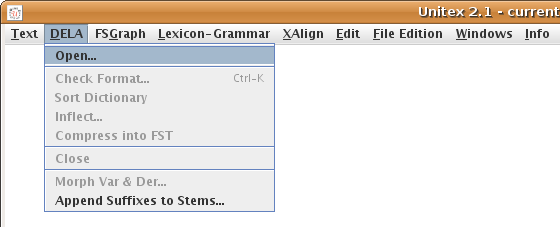
\includegraphics[width=13cm]{resources/img/fig3-1.png}
\caption{Menu "DELA"}
\end{center}
\end{figure}

\bigskip
\noindent
Si vous avez ouvert un dictionnaire, la fenêtrre affichée contient un champ qui vous permet
d'effectuer une recherche. Si le mot apparaît dans le dictionnaire, le bouton "Find" surligne la
première entrée correspondante. Si plusieurs entrées correspondent, vous pouvez les parcourir en
cliquant sur les deux boutons en forme de flèche.

\begin{figure}[h!]
\begin{center}
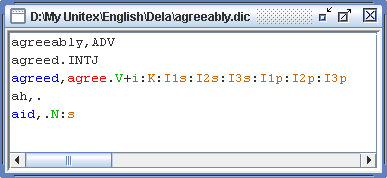
\includegraphics[width=7cm]{resources/img/fig3-2.png}
\caption{Recherche d'un mot dans un dictionnaire}
\end{center}
\end{figure}

\bigskip
\noindent
Vous pouvez aussi rechercher un mots dans plusieurs dictionnaires en cliquant sur le bouton "Lookup" du menu "DELA". Vous pouvez ensuite sélectionner les dictionnaires dans lesquels rechercher le mot que vous avez entré.

\begin{figure}[h!]
\begin{center}
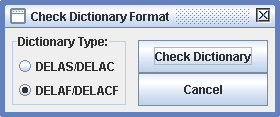
\includegraphics[width=7cm]{resources/img/fig3-3.png}
\caption{Recherche d'un mot dans plusieurs dictionnaires}
\end{center}
\end{figure}

\bigskip
\noindent

%%%%%%%%%%%%%%%%%%




\section{Vérification du format d’un dictionnaire}
\index{Dictionnaire!vérification} \index{Vérification du format d’un dictionnaire}
Lorsque les dictionnaires sont de taille importante, il devient fastidieux de les vérifier à
la main. Unitex contient le programme \verb+CheckDic+\index{Programmes externes!\verb+CheckDic+}
\index{\verb+CheckDic+} qui vérifie automatiquement les dictionnaires DELAF et DELAS.

\bigskip
\noindent Ce programme effectue une vérification de la syntaxe des entrées. Pour chaque entrée
mal formée, le programme affiche le numéro de ligne, le contenu de cette ligne et la nature
de l’erreur. Les résultats de l’analyse sont sauvés dans un fichier nommé
\verb+CHECK_DIC.TXT+\index{Fichier!\verb+CHECK_DIC.TXT+} qui est affiché une fois la vérification
terminée. En plus des éventuels messages d’erreurs, ce fichier contient la liste de tous les
caractères utilisés dans les formes fléchies et canoniques, la liste des codes grammaticaux et
sémantiques,ainsi que la liste des codes flexionnels utilisés.
La liste des caractères permet de vérifier que les caractères présents dans le dictionnaire
sont cohérents avec ceux présents dans le fichier alphabet de la langue. Chaque caractère est
suivi par sa valeur en notation hexadécimale. Les listes de codes peuvent être utilisées pour
vérifier qu’il n’y a pas de faute de frappe dans les codes du dictionnaire.
\index{Fichier!alphabet}


\bigskip
\noindent Le programme \verb+CheckDic+ fonctionne avec des dictionnaires non comprimés, c’est-à-dire
sous forme de fichiers texte. La convention généralement appliquée est de donner l’extension
\verb+.dic+ \index{Fichier!\verb+.dic+}. Pour vérifier le format d’un dictionnaire, il faut tout
d’abord l’ouvrir en cliquant sur "Open..." dans le menu "DELA".


\begin{figure}[h]
\begin{center}
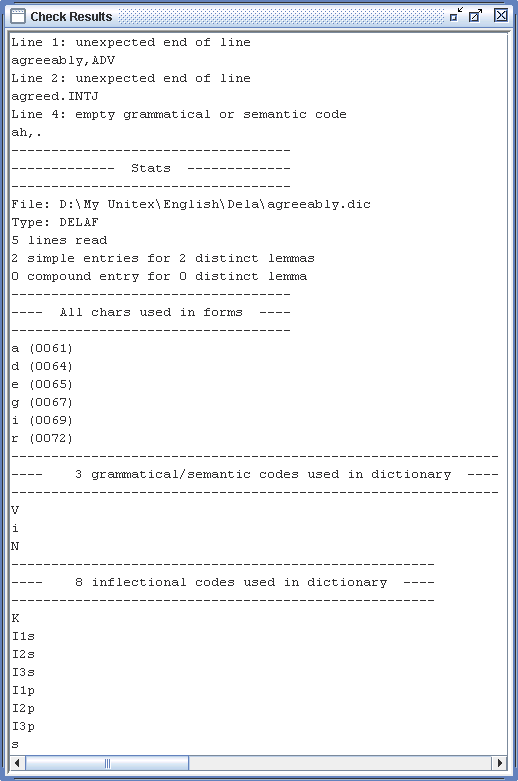
\includegraphics[width=10cm]{resources/img/fig3-4.png}
\caption{Exemple de dictionnaire\label{fig-dictionary-example}}
\end{center}
\end{figure}

\noindent Chargeons le dictionnaire de la figure~\ref{fig-dictionary-example}.
Pour lancer la vérification automatique, cliquez sur "Check Format..." dans le menu "DELA".
la fenêtre de la figure ~\ref{fig-dictionary-checking} apparaît alors.
Cette fenêtre vous permet de choisir le type du dictionnaire que vous voulez vérifier. Les
résultats de la vérification du dictionnaire de la figure~\ref{fig-dictionary-example},
 sont présentés sur la figure~\ref{fig-dictionary-checking-results}.

\bigskip
\noindent La première erreur est due au fait que le programme n’ait pas trouvé de point.
Le seconde, au fait qu’il n’ait pas trouvé de virgule marquant la fin de la forme fléchie.
La troisième erreur indique que le programme n’a trouvé aucun code grammatical ou sémantique.




\begin{figure}[!h]
\begin{center}
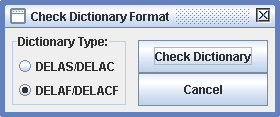
\includegraphics[width=7cm]{resources/img/fig3-5.png}
\caption{Vérification automatique d’un dictionnaire\label{fig-dictionary-checking}}
\end{center}
\end{figure}

\begin{figure}[!p]
\begin{center}
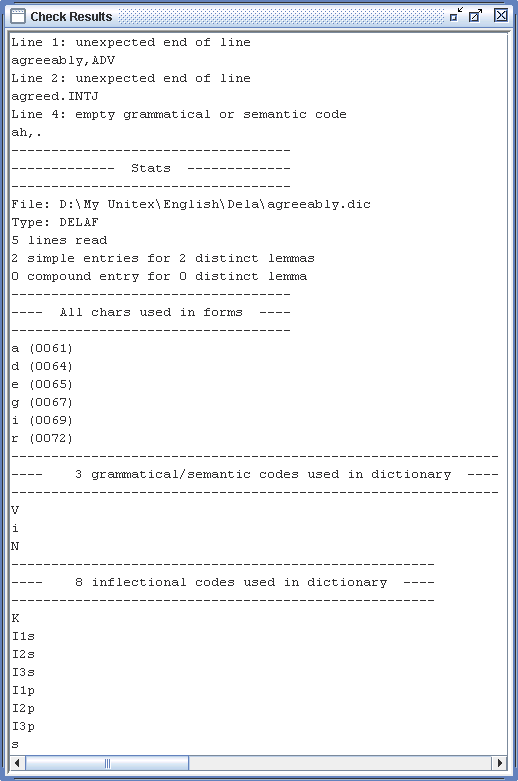
\includegraphics[height=19.4cm]{resources/img/fig3-6.png}
\caption{Résultats d’une vérification automatique\label{fig-dictionary-checking-results}}
\end{center}
\end{figure}


\section{Tri}
\index{Dictionnaires!tri}\index{Trier!un dictionnaire}

Unitex manipule les dictionnaires sans se soucier de l’ordre des entrées. Toutefois, pour
des raisons de présentation, il est souvent préférable de trier les dictionnaires. L’opération
de tri varie selon plusieurs critères, à commencer par la langue du texte à trier. Ainsi, le
tri d’un dictionnaire thaï s’effectue selon un ordre différent de l’ordre alphabétique, si bien
qu’Unitex utilise un mode de tri développé spécialement pour le thaï (voir chapitre
 \ref{chap-external-programs}).

\bigskip
\noindent Pour les langues européennes, le tri s’effectue généralement selon l’ordre
lexicographique, avec toutefois quelques variantes. En effet, certaines langues comme le français
considèrent certains caractères comme équivalents. Par exemple, la différence entre les caractères
\verb+e+ et \texttt{é} est ignorée lorsque l’on veut comparer les mots \verb+manger+ et
\texttt{mangés}, car les contextes \verb+r+ et \verb+s+ permettent de décider de l’ordre. La
distinction n’est faite que lorsque les contextes sont identiques, ce qui est le cas si l’on
compare \texttt{pêche} et \texttt{pèche}.

\bigskip \index{Alphabet!tri}
\noindent
Afin de prendre en compte ce phénomène, le programme de tri \verb+SortTxt+  
\index{\verb+SortTxt+}\index{Programmes externes!\verb+SortTxt+} utilise un fichier qui définit des
équivalences de caractères. \index{Equivalence de caractères}  Ce fichier s’appelle
\verb+Alphabet_sort.txt+ \index{Fichier!\verb+Alphabet_sort.txt+} et se trouve dans le répertoire
de la langue courante de l’utilisateur. Voici les premières lignes du fichier utilisé par défaut
pour le français :


\bigskip
\noindent
\texttt{AÀÂÄaàâä}

\noindent
\texttt{Bb}

\noindent
\texttt{CÇcç}

\noindent
\texttt{Dd}

\noindent
\texttt{EÉÈÊËeéèêë}


\bigskip
\noindent Les caractères présents sur une même ligne sont considérés comme équivalents quand
le contexte le permet. Lorsqu’il faut comparer deux caractères équivalents, on les compare
selon l’ordre dans lequel ils apparaissent de gauche à droite sur la ligne. On peut voir sur
l’extrait ci-dessus qu’on ne fait pas de différence entre minuscules et majuscules, et qu’on
ignore les accents ainsi que la cédille.


\bigskip
\noindent Pour trier un dictionnaire, ouvrez-le, puis cliquez sur "Sort Dictionary" dans le menu
"DELA". Par défaut, le programme cherche toujours à utiliser le fichier \verb+Alphabet_sort.txt+.
Si ce fichier est absent, le tri se fait selon l’indice des caractères dans le codage Unicode.
En modifiant ce fichier, vous pouvez définir vos propres préférences de tri.


\bigskip
\noindent Remarque : après l’application des dictionnaires sur un texte, les fichiers
\verb+dlf+, \verb+dlc+ et \verb+err+ sont automatiquement triés avec ce programme.
\index{Fichier!\verb+dlf+} \index{Fichier!\verb+dlc+}\index{Fichier!\verb+err+}



\section{Flexion automatique}
\label{section-automatic-inflection}
\index{Flexion automatique}\index{Conjugaison}\index{Déclinaison}\index{Dictionnaires!flexion automatique}
\subsection{Flexion des mots simples}

Comme décrit dans la section~\ref{section-DELAS-format}, une ligne de DELAS se compose généralement
d’une forme canonique et d’une séquence de codes grammaticaux ou sémantiques :


\begin{verbatim}
aviatrix,N4+Hum
matrix,N4+Math
radix,N4
\end{verbatim}

\bigskip
\noindent Le premier code rencontré est interprété comme le nom de la grammaire à utiliser pour
fléchir la forme canonique. Il y a deux formes possibles :

\begin{itemize}
\item \verb+N4+: nom de la grammaire=\verb+N4.fst2+, codes grammaticaux=\verb+N+
	(le plus long préfixe uniquement composé de lettres)
  \item \verb+N(NC_XXX)+: nom de la grammaire=\verb+NC_XXX.fst2+, codes grammaticaux=\verb+N+
\end{itemize}

\bigskip
\noindent Ces grammaires de flexion\index{Grammaires!de flexion} seront automatiquement compilées si
besoin est. Dans l’exemple ci-dessus, toutes les entrées seront fléchies avec une grammaire nommée
\verb+N4+.

\bigskip
\noindent Pour lancer la flexion, cliquez sur "Inflect..." dans le menu "DELA". La fenêtre de la 
figure~\ref{fig-inflection-configuration} permet d’indiquer au programme de flexion le
répertoire dans lequel se trouvent les grammaires de flexion. Par défaut, le sous-répertoire
\verb+Inflection+ du répertoire de la langue courante est utilisé. On peut aussi spécifier quels
types de mots le dictionnaire est supposé contenir. Si une entrée non conforme est
rencontrée, un message d'erreur sera affiché.

\bigskip
\begin{figure}[h]
\begin{center}
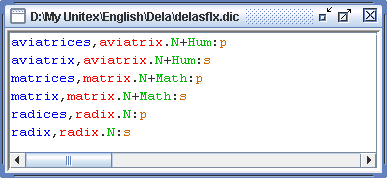
\includegraphics[width=8cm]{resources/img/fig3-7.png}
\caption{Configuration de la flexion automatique\label{fig-inflection-configuration}}
\end{center}
\end{figure}

\bigskip
\begin{figure}[h]
\begin{center}
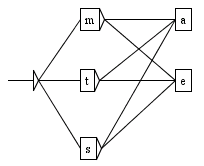
\includegraphics[width=4.5cm]{resources/img/fig3-8.png}
\caption{Grammaire de flexion
\texttt{N4}\label{fig-example-inflectional-grammar}}
\end{center}
\end{figure}

\bigskip
\noindent La figure~\ref{fig-example-inflectional-grammar} présente un exemple de grammaire de
flexion. Les chemins décrivent les suffixes à ajouter ou à retrancher pour obtenir la forme fléchie
à partir de la forme canonique, et les sorties (texte en gras sous les boîtes) donnent les codes
flexionnels à ajouter à l’entrée du dictionnaire.


\bigskip
\noindent Dans notre exemple, deux chemins sont possibles. Le premier ne modifie pas la forme
canonique et ajoute le code flexionnel \verb+:s+. Le second retranche une lettre grâce à l’opérateur 
\verb+L+, ajoute ensuite le suffixe \verb+ces+ et ajoute le code flexionnel \verb+:mp+.

Voici les opérateurs utilisables:

\index{\verb+L+}\index{Opérateur!\verb+L+}\index{\verb+R+}\index{Opérateur!\verb+R+}
\index{\verb+C+}\index{Opérateur!\verb+C+}\index{\verb+D+}\index{Opérateur!\verb+D+}
\index{\verb+U+}\index{Opérateur!\verb+U+}
\index{\verb+P+}\index{Opérateur!\verb+P+}
\index{\verb+W+}\index{Opérateur!\verb+W+}
\index{\verb+J+}\index{Opérateur!\verb+J+}
\index{\verb+.+}\index{Opérateur!\verb+.+}
\index{\verb+<R=?>+}\index{Opérateur!\verb+<R=?>+}
\index{\verb+<I=?>+}\index{Opérateur!\verb+<I=?>+}
\index{\verb+<X=n>+}\index{Opérateur!\verb+<X=n>+}

\begin{itemize}
\item \verb+L+ (left) enlève une lettre à l’entrée;
  	  
\item \verb+R+ (right) rétablit une lettre de l’entrée. En français, beaucoup de verbes du premier
  	  groupe se conjuguent au présent à la troisième personne du singulier en retirant le
  	  \verb+r+ de l’infinitif et en changeant la 4$\ieme$ lettre en partant de la fin en
  	  \texttt{è}: \verb+peler+ $\rightarrow$ \texttt{pèle},
  	  \verb+acheter+ $\rightarrow$ \texttt{achète}, \texttt{gérer}
  	  $\rightarrow$ \texttt{gère}, etc. Plutôt que d’écrire un suffixe de flexion
  	  pour chaque verbe (\texttt{LLLLèle}, \texttt{LLLLète} and
  	  \texttt{LLLLère}), on peut utiliser l’opérateur \verb+R+ pour n’en écrire qu’un seul :
  	  \texttt{LLLLèRR}.
  	  
\item \verb+C+ (copy) duplique une lettre de l’entrée, en décalant tout ce qui se trouve à sa
  	  droite.
  	  
Supposons par exemple que l’on souhaite générer automatiquement des adjectifs en
\verb+able+ à partir de noms. Dans des cas comme \verb+regrettable+ ou \verb+réquisitionnable+,
  on observe un doublement de la consonne finale du nom. Pour éviter d’écrire un
graphe de flexion pour chaque consonne finale possible, on peut utiliser l’opérateur
\verb+C+ afin de dupliquer la consonne finale, quelle qu’elle soit;
  
  \item \verb+D+ (delete) supprime une lettre de l’entrée, en décalant tout ce qui se trouve à sa
  	  droite.
Si l’on souhaite par exemple fléchir le mot roumain \verb+european+ en \verb+europeni+, on utilisera
la séquence \verb+LDRi+. Le \verb+L+ positionnera le curseur sur la lettre \verb+a+, \verb+D+ va
supprimer le \verb+a+, en décalant le \verb+n+ sur la gauche, puis \verb+Ri+ va rétablir le \verb+n+
et ajouter un \verb+i+.

\item \verb+U+ (unaccent) enlève l'accent du caractère courant s'il en comporte un.
	Par exemple la séquence \verb+LLUx+ appliquée au mot
	\texttt{mangés} produit la forme fléchie \verb+mangex+, puisque \verb+U+
	à transformé le \texttt{é} en \verb+e+.

\item \verb+P+ (uppercase) met en majuscule la première lettre de la pile. Par exemple, la séquence
	\verb$Px$ transforme \verb$foo$ en \verb$Foox$.
  
\item \verb+W+ (lowercase) met en minuscule la première lettre de la pile.

\item \verb+<R=?>+ remplace la première lettre de la pile par la lettre \verb+?+.

\item \verb+<I=?>+ insère la lettre \verb+?+ avant la première lettre de la pile 

\item \verb+<X=n>+ supprime les $n$ premières lettres de la pile.
\end{itemize}

\noindent Il y a également deux opérateurs spéciaux pour le  Coréen:
\begin{itemize}\index{Jamo}\index{Hangul}
\item \verb+J+ supprime une lettre Jamo. Si le caractère est un Hangul, ce caractère est d'abord
remplacé par sa séquence équivalente en alphabet Jamo, ensuite, la dernière lettre Jamo est
supprimée. Si le caractère n'est ni un Jamo, ni un Hangul, une erreur est produite.
\item \verb+.+ (latin dot) insère une limite de syllabe. Ceci a un effet de ford, si le haut de la
	pile contient des lettres Jamo, elles sont recombinées en Hangul.
\end{itemize}


\bigskip
\noindent Voici un exemple qui décrit la flexion de \verb+choose+ en \verb+chosen+
      grâce à la séquence d’opérateurs \verb+LLDRRn+ :
\begin{itemize}
  \item Étape 0: initialisation de la pile avec la forme canonique; on place le curseur après la
  	  dernière lettre:

\begin{center}
\begin{tabular}{|l|l|l|l|l|l|l|l}
\multicolumn{6}{l}{} & \multicolumn{2}{l}{$\downarrow$} \\
\hline
\verb+c+ & \verb+h+ & \verb+o+ & \verb+o+ & \verb+s+ & \verb+e+ & \verb+ + & \\
\hline
\end{tabular}
\end{center}

\bigskip
\item Étape 1: on décale le curseur vers la gauche:

\begin{center}
\texttt{\textbf{L}LDRRn}

\begin{tabular}{|l|l|l|l|l|l|l|l}
\multicolumn{5}{l}{} & \multicolumn{3}{l}{$\downarrow$} \\
\hline
\verb+c+ & \verb+h+ & \verb+o+ & \verb+o+ & \verb+s+ & \verb+e+ & \verb+ + & \\
\hline
\end{tabular}
\end{center}

\bigskip
\item Étape 2: on décale une seconde fois le curseur vers la gauche:

\begin{center}
\texttt{\textbf{LL}DRRn}

\begin{tabular}{|l|l|l|l|l|l|l|l}
\multicolumn{4}{l}{} & \multicolumn{4}{l}{$\downarrow$} \\
\hline
\verb+c+ & \verb+h+ & \verb+o+ & \verb+o+ & \verb+s+ & \verb+e+ & \verb+ + & \\
\hline
\end{tabular}
\end{center}

\bigskip \item Étape 3: on décale tout ce qui est à droite du curseur vers la gauche :

\begin{center}
\texttt{\textbf{LLD}RRn}

\begin{tabular}{|l|l|l|l|l|l|l|l}
\multicolumn{3}{l}{} & \multicolumn{5}{l}{$\downarrow$} \\
\hline
\verb+c+ & \verb+h+ & \verb+o+ & \verb+s+ & \verb+e+ & \verb+ + & \verb+ + & \\
\hline
\end{tabular}
\end{center}

\bigskip
\item Step 4: on décale le curseur vers la droite:

\begin{center}
\texttt{\textbf{LLDR}Rn}

\begin{tabular}{|l|l|l|l|l|l|l|l}
\multicolumn{4}{l}{} & \multicolumn{4}{l}{$\downarrow$} \\
\hline
\verb+c+ & \verb+h+ & \verb+o+ & \verb+s+ & \verb+e+ & \verb+ + & \verb+ + & \\
\hline
\end{tabular}
\end{center}

\bigskip
\item Step 5: on décale encore le curseur vers la droite:

\begin{center}
\texttt{\textbf{LLDRR}n}

\begin{tabular}{|l|l|l|l|l|l|l|l}
\multicolumn{5}{l}{} & \multicolumn{3}{l}{$\downarrow$} \\
\hline
\verb+c+ & \verb+h+ & \verb+o+ & \verb+s+ & \verb+e+ & \verb+ + & \verb+ + & \\
\hline
\end{tabular}
\end{center}

\bigskip
\item Step 6: on écrit un \verb+n+

\begin{center}
\texttt{\textbf{LLDRRn}}

\begin{tabular}{|l|l|l|l|l|l|l|l}
\multicolumn{6}{l}{} & \multicolumn{2}{l}{$\downarrow$} \\
\hline
\verb+c+ & \verb+h+ & \verb+o+ & \verb+s+ & \verb+e+ & \verb+n+ & \verb+ + & \\
\hline
\end{tabular}
\end{center}
\end{itemize}

\bigskip
\noindent Une fois la séquence d’opérateurs épuisée, on prend le contenu de la pile jusqu’avant le
curseur pour former la forme fléchie (ici \verb+chosen+).

\bigskip
\noindent Le programme de flexion \verb+Inflect+ explore tous les chemins de la grammaire de flexion
en engendrant toutes les formes fléchies possibles. Afin d’éviter de devoir remplacer les noms des
grammaires de flexion par de vrais codes grammaticaux dans le dictionnaire obtenu, le programme
remplace ces noms par leurs plus longs préfixes composés de lettres. Ainsi, \verb+N4+ est remplacé
par \verb+N+. En choisissant judicieusement les noms des grammaires de flexion, on peut donc
engendrer directement un dictionnaire prêt à l’emploi.

\bigskip
\noindent La figure \ref{fig-inflection-result} montre le dictionnaire obtenu après flexion du DELAS de notre exemple.

\bigskip
\begin{figure}[!ht]
\begin{center}
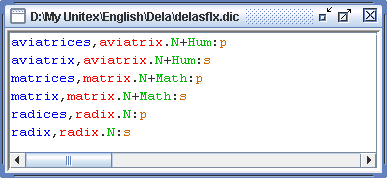
\includegraphics[width=9.5cm]{resources/img/fig3-9.png}
\caption{Résultat de la flexion automatique\label{fig-inflection-result}}
\end{center}
\end{figure}
\bigskip

\subsection{Opérateurs de flexion avancés}
\label{advanced-inflection-operators}
Dans certaines langues le processus de flexion entraine une modification de la racine du mot.
Plusieurs opérateurs ont été développés pour faciliter ce type de traitements. Ils permettent de rechercher
et d'enlever un suffixe du mot \verb+W+ \`a fléchir. Cette opération peut
\^etre accompagnée de la mémorisation dans une variable (\$ ou \pounds) d'un facteur de ce suffixe.
Ces opérateurs peuvent prendre les formes suivantes:

\bigskip
\begin{itemize}
\item \verb+<X$Y>+~: On recherche depuis la fin du mot \verb+W+ la première occurrence de \verb+Y+.
Puis, on recherche \`a partir de la position atteinte la {\bf première} occurrence de \verb+X+ qui
précède strictement celle de \verb+Y+ . La variable \$ contient alors le {\bf plus court facteur}
({\bf\$}hortest) de \verb+W+ strictement compris entre \verb+X+ et \verb+Y+ (\verb+W = U.X.$.Y+) \footnote{Le point
représente ici l'opération de concaténation.}.
\item \verb+<X£Y>+~: On recherche depuis la fin du mot \verb+W+ la première occurrence de \verb+Y+.
Puis, on recherche \`a partir de la position atteinte la {\bf dernière} occurrence de \verb+X+ qui
précède strictement celle de \verb+Y+. La variable {\pounds} contient alors le {\bf plus long facteur}
({\bf£}ongest) de \verb+W+ strictement compris entre \verb+X+ et \verb+Y+ (\verb+W = U.X.£.Y+).
\item \verb+<X>+~: Si aucune variable n'est présente, on recherche \verb+X+ comme suffixe de \verb+W+
	(\verb+W =U.X+).
\item \verb+<$Y>+: Si le facteur \verb+X+ est absent, le {\bf plus court facteur \verb+$+} est la première lettre
	qui précède strictement \verb+Y+ .
\item \verb+<£Y>+~: Si le facteur \verb+X+ est absent, le {\bf plus long facteur \verb+£+} est le préfixe de
	\verb+W+ tel que  \verb+W = £.Y+.
\end{itemize}

\bigskip
\noindent
Pour illustrer l'utilisation des ces opérateurs, considérons le verbe {\it reprendre}~:

\bigskip
\begin{center}
\begin{tabular}{|l|l|l|l|}
\hline
Verbe     & Opérateur & Variable & Résultat\\
\hline
\hline
reprendre & <re> & & reprend\\
reprendre & <\$> & \$ = e & reprendr\\
reprendre & <{\pounds}> &{\pounds}= reprendre & $\varepsilon$ \\
reprendre & <re\$re> & \$ = nd & rep\\
reprendre & <re{\pounds}re> & {\pounds} = prend & \\
reprendre & <\$re> & \$ = d & repren\\
reprendre & <re\$> & \$ =  $\varepsilon$ & reprendre\\
reprendre & <{\pounds}re> & {\pounds} = reprend & $\varepsilon$\\
reprendre & <re{\pounds}> & {\pounds} = prendre & re\\
\hline
\end{tabular}
\end{center}

\bigskip
\noindent
Le programme MultiFlex permet d'utiliser dix variables de type \$ dont les noms sont \$,\$1,...,\$9
et dix variables de type {\pounds} dont les noms sont {\pounds},{\pounds}1,...,{\pounds}9. De plus,
plusieurs variables de types différents peuvent \^etre utilisées au sein d'une m\^eme opération.
Ainsi l'opérateur <{\pounds}3re\$7re> appliqué au verbe {\it reprendre} donne~: {\pounds}3 = 
 rep et \$7 = \verb+nd+.

\bigskip
\noindent
Si l'on considère les verbes \verb+accélérer+, \verb+sécher+, la
deuxième personne du présent de l'indicatif peut \^etre générée par l'opération <é\$er>è\$es~:

\begin{center}
\begin{tabular}{lllllllll}
	\verb+accélérer+ & <é\$er> & $\rightarrow$ & abr & \$ = g & + & è\$es &  $\rightarrow$ & \verb+accélères+\\
	\verb+sécher+ & <é\$er> & $\rightarrow$ & s & \$ = ch & + & è\$es & $\rightarrow$ & \verb+sèches+\\
\end{tabular}
\end{center}

\noindent
On remarque que le facteur \verb+$+ conservé dans la forme fléchie est de longueur variable (\verb+g+, \verb+ch+). 
La flexion de \verb+accélérer+ et \verb+sécher+ ne peut se faire que par des opérateurs de pile
classiques \`a l'aide d'une opération commune. Deux opérations différentes (\verb+-4RèCes+, \verb+-5RèCes+) sont
nécessaires. Le graphe de la figure~\ref{fig-inflection-secher} permet de fléchir des verbes comme
\verb+accélérer+ et \verb+sécher+ au présent.

\begin{figure}[!ht]
\begin{center}
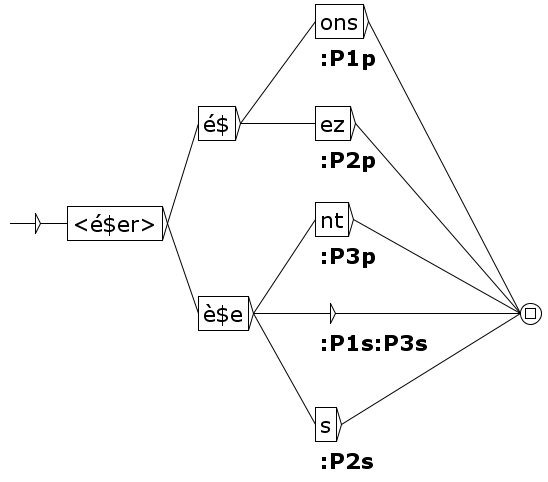
\includegraphics[width=7cm]{resources/img/fig3-Advanced_operators_with_Variables-V_secher.png}
\caption{Graphe de flexion pour des verbes comme {\it accélérer}, {\it sécher}
\label{fig-inflection-secher}}
\end{center}
\end{figure}

\newpage
\noindent
Voici les flexions obtenues pour les verbes \verb+accélérer+ et \verb+sécher+:

\begin{figure}[!ht]
\begin{center}
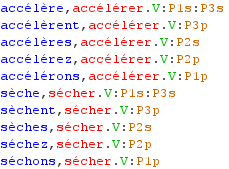
\includegraphics[width=5cm]{resources/img/fig3-flexion_secher.png}
\end{center}
\end{figure}

\bigskip
\noindent
Le redoublement de certaines lettres lors de la flexion peut s'effectuer avec l'opérateur \$.
Par exemple l'adject {\it tranquil} en anglais possède deux formes au comparatif et deux au
superlatf. Le graphe de la figure ~\ref{fig-inflection-tranquil} permet de les produire.

\bigskip
\begin{figure}[!ht]
\begin{center}
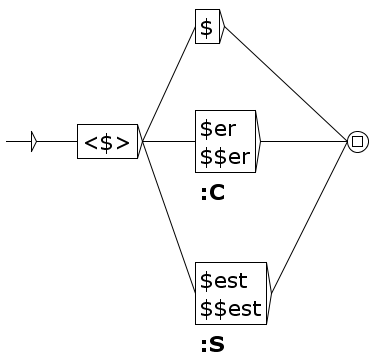
\includegraphics[width=5.5cm]{resources/img/fig3-Advanced_operators_with_Variables-A_tranquil.png}
\caption{Graphe de flexion pour des adjectifs anglais comme {\it tranquil}
\label{fig-inflection-tranquil}}
\end{center}
\end{figure}

\noindent Voici les flexions obtenues pour l'adjectif anglais \verb+tranquil+:

\bigskip
\begin{figure}[!ht]
\begin{center}
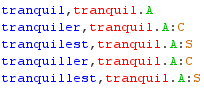
\includegraphics[width=5cm]{resources/img/fig3-flexion_tranquil.png}
\end{center}
\end{figure}

\noindent Dans certaines langues, certaines formes fléchies comporte un préfixe qui s'ajoute devant la racine.
C'est le cas lors de la formation du participe passé en allemand. L'utilisation conjointe des
opérateurs \verb+£+ et \verb+$+ permet de fléchir le verbe allemand \verb+sprechen+ (parler)
au présent et participe passé comme le montre le graphe de la figure~\ref{fig-inflection-sprechen}.

\newpage
\begin{figure}[!htbp]
\begin{center}
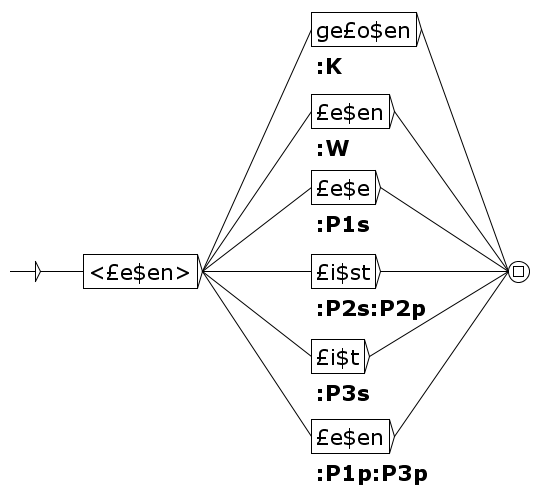
\includegraphics[width=5cm]{resources/img/fig3-Advanced_operators_with_Variables-V_sprechen.png}
\caption{Graphe de flexion pour des verbes comme {\it sprechen}
\label{fig-inflection-sprechen}}
\end{center}
\end{figure}

\noindent Voici les flexions obtenues pour le verbe allemand \verb+sprechen+:

\bigskip
\begin{figure}[!ht]
\begin{center}
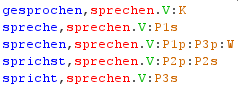
\includegraphics[width=5cm]{resources/img/fig3-flexion_sprechen.png}
\end{center}
\end{figure}

\noindent Si l'on veut fléchir le verbe à particule aussprechen on peut utiliser deux variables de type \$.
Le figure ~\ref{fig-inflection-aussprechen} montre un graphe qui comport les variables \verb+$1+ et \verb+$2+.

\bigskip
\begin{figure}[!ht]
\begin{center}
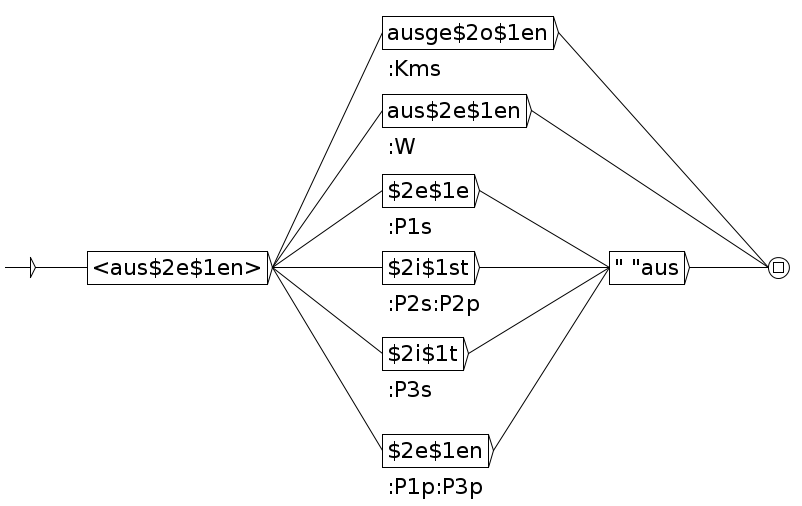
\includegraphics[width=10.5cm]{resources/img/fig3-Advanced_operators_with_Variables-V_aussprechen.png}
\caption{Graphe de flexion pour des verbes comme {\it aussprechen}
\label{fig-inflection-aussprechen}}
\end{center}
\end{figure}

\noindent Voici les flexions obtenues pour le verbe allemand \verb+aussprechen+:
\bigskip
\begin{figure}[!ht]
\begin{center}
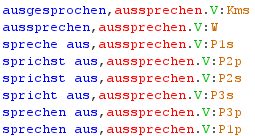
\includegraphics[width=5cm]{resources/img/fig3-flexion_aussprechen2.png}
\end{center}
\end{figure}

\bigskip
\noindent \textbf{Codes sémantiques}
\noindent Dans certaines langues, il existe des caractéristiques flexionnelles qui correspondent
en fait à des caractéristiques sémantiques comme par exemple les marqueurs de la forme passive.
Ces codes peuvent ne pas apparaître comme des codes flexionnels, mais plutôt comme des codes
sémantiques. Pour produire des codes sémantiques, il faut insérer un signe plus au début de la
sortie d'une boîte. Cette boîte doit seulement contenir le code sémantique précédé d'un plus, comme
le montre la figure~\ref{fig-inflection-sem}.

\bigskip
\begin{figure}[!ht]
\begin{center}
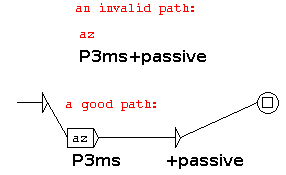
\includegraphics[width=6cm]{resources/img/fig3-9sem.png}
\caption{Une grammaire de flexion avec un code sémantique\label{fig-inflection-sem}}
\end{center}
\end{figure}

\subsection{Flexion des mots composés}
Voir chapitre \ref{chap-multiflex}.

\subsection{Flexion des langues sémitiques}
\label{subsection-semitic-inflection}
\index{Langues sémitiques}
Les langues  sémitiques comme l'arabe ou l'hébreu ne se fléchissent pas de la même manière 
que d'autres types de langues. Leur morphologie obéit à une logique différente.
Dans ces langues, les mots se fléchissent selon un \textit{squelette consonantique}\index{Squelette consonantique}. Le processus de
flexion combine ce squelette avec des voyelles.

\bigskip
\noindent Tout d'abord, voyons un cas où on ne code que les consonnes dans le champ lemme de l'entrée DELAS~:

\bigskip
\noindent \verb+ktb,$V31-123+

\bigskip
\noindent Le signe \verb+$+ avant le code grammatical indique que la grammaire de flexion est en mode sémitique, et
la forme \verb+ktb+ qui figure dans le champ lemme est le squelette consonantique. La figure \ref{semitic-grammar}
montre une grammaire jouet \verb+V31-123.grf+ qui illustre comment le mode sémitique fonctionne.

\bigskip
\begin{figure}[!ht]
\begin{center}
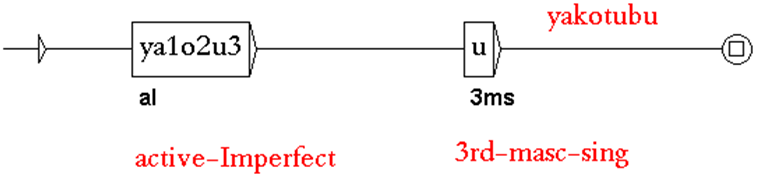
\includegraphics[width=10cm]{resources/img/fig3-15.png}
\caption{Une grammaire de flexion jouet en mode sémitique\label{semitic-grammar}}
\end{center}
\end{figure}

\bigskip
\noindent Le mode sémitique obéit aux règles suivantes:
\begin{enumerate}
\item Tous les opérateurs standards de flexion peuvent être utilisés (\verb+L+, \verb+R+, etc.).
\item Un chiffre représente une lettre du champ lemme (\verb+1+ pour la première,
\verb+2+ pour la seconde, etc). Dans notre exemple, \verb+1+, \verb+2+ et \verb+3+ représentent
respectivement \verb+k+, \verb+t+ et \verb+b+. Si on veut désigner une lettre après la neuvième,
on doit protéger son numéro avec des chevrons~: \verb+<10>+.
\end{enumerate}  

\bigskip
\noindent Le DELAF produit par cette grammaire est:\\ 
  
\verb+yakotubu,ktb.V:aI3ms+

\bigskip
\noindent Si on ne code que les consonnes dans le champ lemme et que deux entrées ont les mêmes consonnes et diffèrent par leurs voyelles, on doit coder les voyelles dans les grammaires de flexion~:\\ 

\verb+Hsb,$V3au	// compter, Hasaba, yaHosubu+

\verb+Hsb,$V3ii	// penser, Hasiba, yaHosibu+

\bigskip
\noindent Pour copier tout le champ lemme, utilisez l'opérateur <LEMMA> (figure~\ref{LEMMA-operator}). De cette façon, un chemin avec tout le champ lemme ne dépend pas du nombre de lettres.
Cet opérateur est utile pour les noms et adjectifs arabes pour lesquels les formes du masculin sont obtenues en
insérant des voyelles dans le squelette consonantique, alors que celles du féminin le sont en ajoutant des
suffixes. Dans cet exemple, on a codé à la fois les consonnes et les voyelles dans le champ lemme.

\begin{figure}[!ht]
\begin{center}
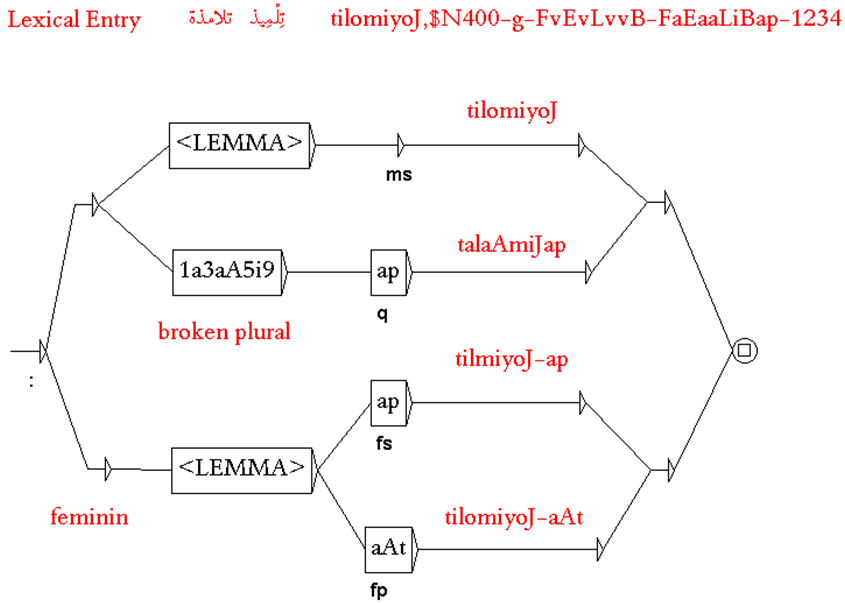
\includegraphics[width=10cm]{resources/img/fig3-LEMMA-operator.png}
\caption{Une grammaire de flexion en mode sémitique avec l'opérateur <LEMMA>\label{LEMMA-operator}}
\end{center}
\end{figure}

\section{Compression}
\index{Dictionnaires!compression}

Unitex applique aux textes des dictionnaires comprimés. La compression permet de réduire
la taille des dictionnaires et d’en accélérer la consultation. Cette opération s’effectue
avec le programme \verb+Compress+. \index{\verb+Compress+}\index{Programmes externes!\verb+Compress+}
Celui-ci prend en entrée un dictionnaire sous forme de fichier texte (par exemple
	\verb+mon_dico.dic+) et produit deux fichiers:\index{Fichier!\verb+.dic+}

\begin{itemize}
  \item \verb+mon_dico.bin+ contient l’automate minimal des formes fléchies du dictionnaire;
  	  \index{Fichier!\verb+.bin+}
  \item \verb+mon_dico.inf+ \index{Fichier!\verb+.inf+}contient des codes qui permettent de
  	  reconstruire le dictionnaire d’origine à partir
  	  des formes fléchies contenues dans \verb+mon_dico.bin+.
\end{itemize}

\index{Automate!minimal}
\noindent L’automate minimal contenu dans \verb+mon_dico.bin+ est une représentation des formes
fléchies où tous les préfixes et suffixes
communs sont factorisés. Par exemple, l’automate minimal des mots \verb+me+, \verb+te+, \verb+se+,
\verb+ma+, \verb+ta+ et \verb+sa+
peut être représenté par le graphe de la figure~\ref{fig-example-minimal-automaton}.
\bigskip \begin{figure}[!h]
\begin{center}
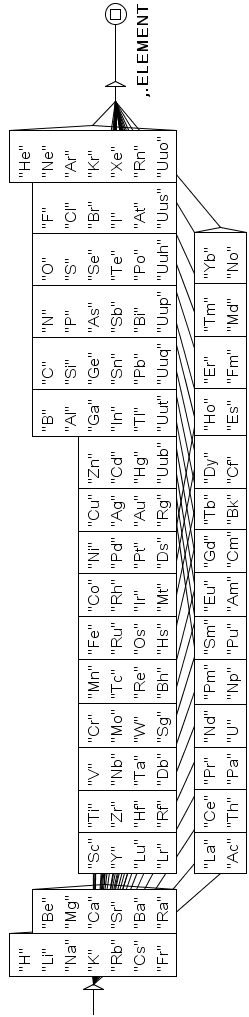
\includegraphics[width=5cm]{resources/img/fig3-10.png}
\caption{Représentation d’un exemple d’automate minimal\label{fig-example-minimal-automaton}}
\end{center}
\end{figure}

\noindent    Pour comprimer un dictionnaire, ouvrez-le puis cliquez sur "Compress into FST" dans le
menu "DELA". La compression est indépendante de la langue et du contenu du dictionnaire.
Les messages produits par le programme sont affichés dans une fenêtre qui ne se ferme pas
automatiquement. Vous pouvez ainsi voir la taille du fichier
\verb+.bin+, obtenu, le nombre de lignes lues ainsi que le nombre de codes flexionnels produits. La
figure ~\ref{fig-compression-result}
montre le résultat de la compression d’un dictionnaire de mots simples.

\bigskip
\begin{figure}[!h]
\begin{center}
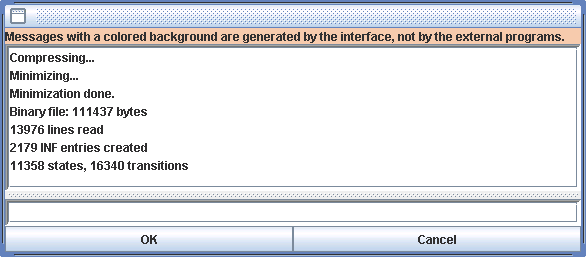
\includegraphics[width=14cm]{resources/img/fig3-11.png}
\caption{Résultat d’une compression\label{fig-compression-result}}
\end{center}
\end{figure}

\bigskip
\noindent À titre indicatif, les taux de compression généralement observés sont d’environ 95\% pour
les dictionnaires de mots simples et 50\% pour ceux de mots composés.


\bigskip
\noindent REMARQUE : pour les langues sémitiques, un algorithme de compression particulier est utilisé
afin de réduire la taille des fichiers \verb+.bin+ et \verb+.inf+. Le fait qu'une langue soit
considérée comme sémitique peut être configuré dans les préférences globales.


\section{Application de dictionnaires}
\label{section-applying-dictionaries}
\index{Dictionnaires!application}

\bigskip
\noindent Unitex peut manipuler soit des dictionnaires compressés (\verb+.bin+) soit des graphes
dictionnaires (\verb+.fst2+). Ces dictionnaires peuvent être appliqués soit lors du prétraitement,
soit explicitement en cliquant sur "Apply Lexical Resources..." dans le menu "Text". Nous allons
maintenant détailler les règles de l’application des dictionnaires. Le cas des graphes dictionnaires
sera abordé dans la section ~\ref{section-dictionary-graphs}.

\subsection{Priorités}
\label{section-dictionary-priorities}
\index{Dictionnaires!priorité}\index{Priorité!des dictionnaires}
La règle de priorité est la suivante : si un mot du texte a été trouvé dans un dictionnaire,
ce mot ne sera plus pris en compte lors de l’application de dictionnaires ayant une priorité
inférieure.


\bigskip
\noindent Cela permet d’éliminer certaines ambiguïtés lors de l’application des dictionnaires.
Par exemple, le mot \textit{par} a une interprétation nominale dans le domaine du golf. Si l’on ne
veut pas envisager cet emploi, il suffit de créer un dictionnnaire filtre ne contenant que l’entrée 
\verb$par,.PREP$ et de le sauver en lui donnant la priorité la plus haute. De cette manière, même
si le dictionnaire des mots simples contient l’autre entrée, celle-ci sera ignorée grâce au jeu
des priorités.

\index{Dictionnaires!filtres}

\bigskip
\noindent Il y a trois niveaux de priorités. Les dictionnaires dont les noms sans extension se
terminent par \verb+-+\index{\verb+-+}\index{\verb-+-} ont la priorité la plus grande ; ceux dont
le nom se termine par \verb-+- ont la priorité la plus faible ; les autres dictionnaires sont
appliqués avec une priorité moyenne. L’ordre d’application de plusieurs dictionnaires ayant la même
priorité est sans importance. En ligne de commande, l’instruction :


\bigskip
\noindent
\verb$Dico ex.snt alph.txt ctr+.bin cities-.bin rivers.bin regions-.bin$

\bigskip \noindent appliquerait donc les dictionnaires dans l’ordre suivant (\verb+ex.snt+ est le
texte auquel sont appliqués les dictionnaires, \verb+alph.txt+ est le fichier alphabet utilisé):

\bigskip
\begin{enumerate}
  \item \verb$cities-.bin$
  \item \verb$regions-.bin$
  \item \verb$rivers.bin$
  \item \verb$ctr+.bin$
\end{enumerate}

\subsection{Règles d’application des dictionnaires}
\label{section-transducer-application-rules}

Outre la règle de priorités, l’application des dictionnaires s’effectue en respectant les
majuscules et les espaces. La règle du respect des majucules est la suivante :

\index{Règles!majuscules et minuscules}

\begin{itemize}
  \item s’il y a une majuscule dans le dictionnaire, alors il doit y avoir une majuscule dans le
texte ;

  \item s’il y a une minuscule dans le dictionnaire, il peut y avoir soit une minuscule soit une
majuscule dans le texte.

\end{itemize}

\bigskip
\noindent Ainsi, l’entrée \verb$pierre,.N:fs$ reconnaîtra les mots \verb+pierre+,
\verb+Pierre+ et \verb+PIERRE+, alors que

\noindent \verb$Pierre,.N+Prénom$ ne reconnaîtra que \verb+Pierre+ et \verb+PIERRE+. Les lettres
minuscules et majuscules sont définies par le fichier alphabet passé en paramètre au programme
\verb+Dico+\index{\verb+Dico+}\index{Programmes externes!\verb+Dico+}
\index{Fichier!\verb+alphabet+}.\index{Règles!espace}

\bigskip
\noindent Le respect des espacements est une règle très simple : pour qu’une séquence du texte
soit reconnue par une entrée de dictionnaire, elle doit avoir exactement les mêmes espaces.
Par exemple, si le dictionnaire contient \verb+aujourd'hui,.ADV+, la séquence \verb+Aujourd' hui+
ne sera pas reconnue à cause de l’espace qui suit l’apostrophe.


\subsection{Graphes dictionnaires}
\label{section-dictionary-graphs}\index{Graphes dictionnaires}
Le programme \verb+Dico+\index{\verb+Dico+}\index{Programmes externes!\verb+Dico+} est capable
d’appliquer des graphes dictionnaires. Il s’agit de graphes qui respectent la règle suivante :
si on les applique avec le programme \verb+Locate+\index{\verb+Locate+}\index{Programmes externes!\verb+Locate+} en mode MERGE,\index{MERGE} ils doivent produire des séquences
correspondant à des lignes de DELAF.\index{DELAF}\index{Dictionnaires!DELAF}

\begin{figure}[!p]
\begin{center}
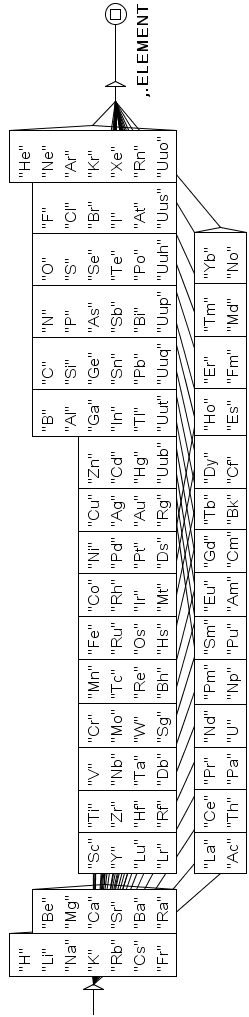
\includegraphics[height=24cm]{resources/img/fig3-12.png}
\caption{Graphe dictionnaire des éléments chimiques\label{elements}}
\end{center}
\end{figure}

\bigskip
\noindent La figure \ref{elements} montre un graphe reconnaissant les symboles chimiques. On peut
voir sur cette figure un premier avantage par rapport aux dictionnaires compressés : l’utilisation
des guillemets permet de forcer le respect de la casse. Ainsi, ce graphe reconnaîtra bien \verb+Fe+
mais pas \verb+FE+, alors qu’il est impossible de spécifier une telle interdiction dans un DELAF
usuel.

\bigskip
\noindent Le second avantage des graphes dictionnaires est qu’ils peuvent exploiter les résultats
fournis par les dictionnaires appliqués précédemment. Ainsi, on peut appliquer le dictionnaire
général, puis étiqueter comme noms propres les mots inconnus commençant par une majuscule à l’aide
du graphe \verb$NPr+$ de la figure~\ref{graph-NPr}. Le \verb$+$ dans le nom du graphe lui donne une
priorité basse afin qu’il soit appliqué après le dictionnaire général. Pour fonctionner, ce graphe
se base sur les mots qui sont toujours inconnus après le passage du dictionnaire général. Les
crochets correspondent à une définition de contexte. Pour plus de détails sur les contextes,
\index{Contexte} voir la section \ref{section-contexts}.

\begin{figure}[!h]
\begin{center}
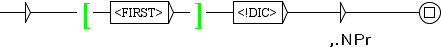
\includegraphics[width=10.5cm]{resources/img/fig3-13.png}
\caption{Graphe dictionnaire étiquetant comme noms propres les mots inconnus commençant par une
majuscule
\label{graph-NPr}}
\end{center}
\end{figure}

\bigskip
\noindent Comme les graphes dictionnaires sont appliqués par le moteur du programme \verb+Locate+,
ils peuvent utiliser tout ce que le programme \verb+Locate+ autorise. En particulier, il est
possible d’utiliser les filtres morphologiques.\index{Filtres morphologiques}\index{Mode
morphologique}
Ainsi, le graphe de la figure \ref{graph-CR} utilise ces filtres pour reconnaître les nombres en
chiffres romains. Notons qu’il utilise également des contextes afin d’éviter, par exemple, que
\verb+C+ ne soit pris comme chiffre romain quand il est suivi par une apostrophe.


\bigskip
\begin{figure}[!p]
\begin{center}
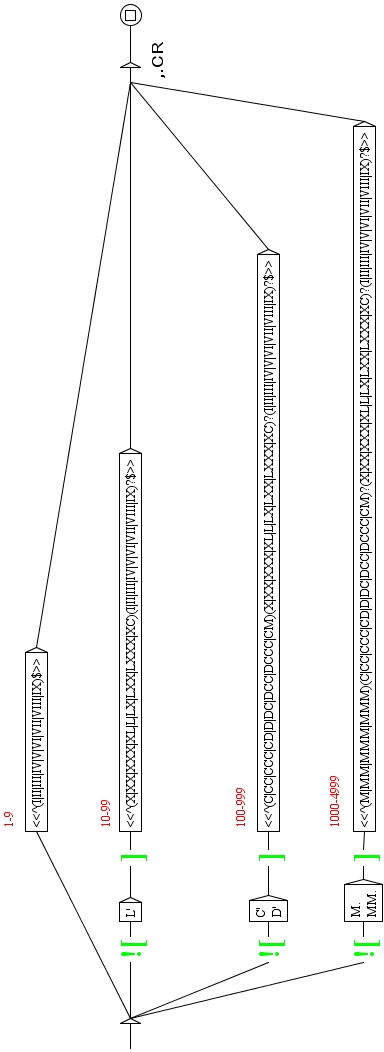
\includegraphics[height=24cm]{resources/img/fig3-14.png}
\caption{Graphe dictionnaire reconnaissant les nombres en chiffres romains\label{graph-CR}}
\end{center}
\end{figure}

\bigskip
\noindent Par défaut, les graphes dictionnaires sont appliqués en mode MERGE. Il est possible 
de les appliquer en mode REPLACE, en ajoutant à leur le nom le suffixe \verb+-r+. Celui-ci se
combine avec les priorités \verb-+- et \verb+-+:

\bigskip
\verb?bagpipe-r.fst2  McAdam-r-.fst2  phtirius-r+.fst2?


\subsubsection{Exporter les entrées produites comme dictionnaire morphologique}
Les entrées produites par un graphe dictionnaire sont, bien sûr, prises en compte
par le programme \verb+Locate+. Cependant, on ne peut les utiliser en mode morphologique
dans la mesure où elles n'appartiennent pas à un dictionnaire morphologique.
Il est possible de le faire en ajoutant \verb+b+ à la fin du nom du graphe dictionnaire. 
Si l'on ajoute \verb+z+ à la place, le dictionnaire morphologique du texte sera immédiatement
compressé le rendant utilisable par le prochain dictionnaire morphologique appliqué.
 
\subsubsection{Conventions de nommage}
Le processus de nommage d'un graphe dictionnaire s'établit comme suit :\\

\verb$nom(-XYZ)([-+]).fst2$\\

\noindent où:
\begin{itemize}
\item \verb+X+ prend l'une des valeurs \verb+[rRmM]+: \verb+r+ signifie mode REPLACE; \verb+M+
signifie mode MERGE (mode par défaut);
\item \verb+Y+ prend l'une des valeurs \verb+[bBzZ]+: option qui régie la construction du
dictionnaire morphologique (voir section précédente);
\item \verb+Z+ prend l'une des valeurs \verb+[aAlLsS]+: \verb+a+ signifie que le graphe est appliqué
en mode "All matches"; \verb+l+ signifie mode "Longest matches" (mode par défault); 
\verb+s+ signifie "Shortest matches".
\end{itemize}


\subsection{Graphe dictionnaire morphologique}
\index{Graphe dictionnaire morphologique}
En plus des graphes dictionnaires  qui produisent de nouvelles entrées dans le dictionnaire du
texte, il est possible de construire des graphes dictionnaires morphologiques.
Les sorties de tels graphes seront utilisées comme entrées pour construire l'automate du texte. Nous
les appelons ``graphes dictionnaires morphologiques'', parce que leur principale utilité est de
fournir de nouvelles analyses morphologiques dans l'automate du texte, grâce au mode morphologique
(voir \ref{section-morphological-mode}). Cette fonctionnalité est très utile pour des langues
agglutinantes comme le coréen.

\bigskip
\noindent La règle est simple: toute sortie du graphe dictionnaire commençant par un  slash 
est ajoutée au fichier \verb+tags.ind+, \index{\verb+tags.ind+} situé dans le répertoire du texte.
Ce fichier est utilisé par le programme \verb+Txt2Fst2+ afin d'ajouter des interprétations à
l'automate du texte. Considérons la grammaire de la figure \ref{morphoA} qui reconnaît des mots
formés par le préfixe \verb+un+ suivi d'un adjectif. Si l'on applique cette grammaire comme graphe
dictionnaire, on obtient de nouveaux chemins dans l'automate du texte comme le montre la figure
\ref{morphoB}. Remarquons que lorsque deux tags correspondent à des analyses dans la même unité lexicale, le lien entre eux est affiché par une ligne discontinue.

\begin{figure}[!ht]
\begin{center}
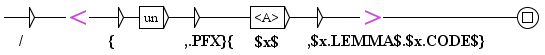
\includegraphics[width=14cm]{resources/img/fig3-14a.png}
\caption{Exemple de graphe dictionnaire morphologique\label{morphoA}}
\end{center}
\end{figure}

\begin{figure}[!ht]
\begin{center}
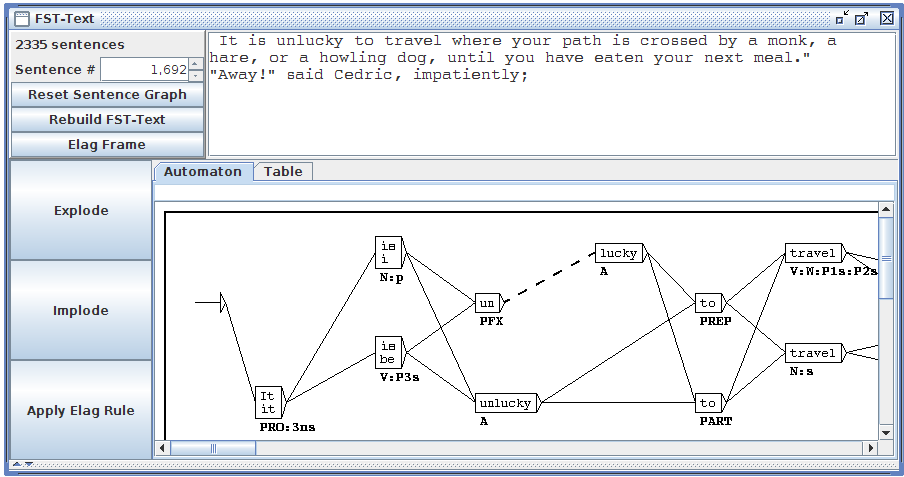
\includegraphics[width=15cm]{resources/img/fig3-14b.png}
\caption{Chemin ajouté par un graphe dictionnaire morphologique\label{morphoB}}
\end{center}
\end{figure}

\section{Bibliographie}

Le tableau ~\ref{ref-dicos} donne quelques références relatives aux dictionnaires électroniques de
mots simples et composés. Pour plus de détails, consultez la page de références sur le site
web d’Unitex: \url{http://www-igm.univ-mlv.fr/~unitex}

\bigskip
\begin{table}[!h]
\begin{center}
\begin{tabular}{|l|c|c|}
\hline
\textbf{Langue} & \textbf{Mots simples} & \textbf{Mots composés} \\
\hline
English & \cite{klarsfeld}, \cite{monceaux-1995} & \cite{delac-anglais},
\cite{these-Savary} \\
\hline
French & \cite{formes-ambigues}, \cite{dicos-francais}, \cite{jacques-1995} & \cite{dicos-francais},
\cite{Gross96},
\cite{max-1993},
\cite{syntaxe-de-ladverbe} \\
\hline
Modern Greek & \cite{modern-greek}, \cite{matthieu-anastasia}, \cite{these-tita} & \cite{tita-2002},
\cite{anastasia-2002} \\
\hline
Italian & \cite{delaf-italien}, \cite{delaf-italien-book} & \cite{composes-italien} \\
\hline
Spanish & \cite{blanco-2000} & \cite{blanco-1997} \\
\hline
Portuguese & \cite{eleuterio1995}, \cite{ranchhod1996b}, \cite{ranchhodd1998},
\cite{muniz2005} & \cite{ranchhod1991}, \cite{ranchhodd1998} \\
\hline
\end{tabular}
\caption{Quelques références bibliographiques sur les dictionnaires électroniques\label{ref-dicos}}
\end{center}
\end{table}

\chapter{Recherche d’expressions rationnelles}
\label{chap-regexp}

Nous allons voir dans ce chapitre comment rechercher des motifs simples dans un texte
au moyen des expressions rationnelles.

\section{Définition}
\index{Expressions rationnelles}

Le but de ce chapitre n’est pas de faire une introduction aux langages formels, mais
de montrer comment utiliser les expressions rationnelles dans Unitex pour rechercher des
motifs simples. Le lecteur intéressé par une présentation plus formelle pourra se reporter
aux nombreux ouvrages qui traitent du sujet.


\bigskip \noindent Une expression rationnelle peut-être:

\begin{itemize}
  \item une unité lexicale (\verb+livre+) ou un masque lexical
  (\verb+<manger.V>+);
  \item une position particulière du texte : le début \verb+{^}+ou la fin \verb+{$}+
  \item la concaténation de deux expressions rationnelles (\verb+je mange+);\index{Concaténation d'expressions rationnelles}
  \item l'union de deux expressions rationnelles (\verb$Pierre+Paul$);\index{Union d'expressions rationnelles} 
  \item l’étoile de Kleene d’une expression rationnelle (\verb+très*+).\index{Etoile de Kleene}
\end{itemize}


\section{Unités lexicales}
\index{Unité lexicale}

Dans une expression rationnelle, l’unité lexicale a la même définition qu’en \ref{tokenization}
(page \pageref{tokenization}). Notons que les symboles point, plus, étoile, inférieur ainsi que les
parenthèses ouvrantes et fermantes ont une signification particulière, il faut donc les
déspécialiser avec le caractère \verb+\+ si l’on souhaite les rechercher. Voici quelques exemples
d’unités lexicales valides: \index{\verb+\+}

\begin{verbatim}
chat
\.
<N:ms>
{S}
\end{verbatim}

\index{Respect de la casse}
\noindent Par défaut, Unitex tolère que des mots avec des minuscules reconnaissent des mots écrits
avec des majuscules. Il est possible de forcer le respect de la casse en utilisant les guillemets.
Ainsi, \verb+"pierre"+ ne reconnaît que la forme \verb+pierre+ et non pas \verb+Pierre+ ou \verb+PIERRE+.

\bigskip
\noindent NOTE: si l’on souhaite rendre la présence d’un espace obligatoire, il faut le mettre entre
guillemets.

\index{Espace!obligatoire}


\section{Motifs}
\index{Masque!lexical}
Un masque lexical est une requête qui reconnaît une unité lexicale ou une suite d'unités lexicales

\subsection{Symboles spéciaux}
\label{section-special-symbols}
\index{Meta-symbols}

Il y a deux sortes de motifs. La première catégorie regroupe tous les symboles présentés à la
section ~\ref{section-sentence-splitting} à l’exception de \verb$<PNC>$, qui reconnaît des signes de
ponctuation, et du symbole \verb+<^>+, qui reconnaît un retour à ligne. Tous les retours à la ligne
ayant été remplacés par des espaces, ce symbole n’a plus aucune utilité lors de la recherche de
motifs. Ces symboles, également appelés \textit{métas}, sont les suivants:


\bigskip
\index{\verb+<MOT>+}\index{\verb+<MIN>+}\index{\verb+<MAJ>+}\index{\verb+<PRE>+}\index{\verb+<NB>+}
\index{\verb+#+}\index{\verb+<E>+}\index{\verb+<DIC>+}\index{\verb+<SDIC>+}\index{\verb+<CDIC>+}
\index{\verb+<TDIC>+}
\begin{itemize}
  \item \verb+<E>+ : mot vide, ou epsilon. Reconnaît la séquence vide;
  \item \verb+<TOKEN>+ : reconnaît n’importe quelle unité lexicale sauf l'espace
  	  utilisé par défaut pour les filtres morphologiques;
  \item \verb+<MOT>+ : reconnaît n’importe quelle unité lexicale formée de lettres;
  \item \verb+<MIN>+ : reconnaît n’importe quelle unité lexicale formée de lettres minuscules;
  \item \verb+<MAJ>+ : reconnaît n’importe quelle unité lexicale formée de lettres majuscules;
  \item \verb+<PRE>+ : reconnaît n’importe quelle unité lexicale formée de lettres et commençant par
  	  une
majuscule;
  \item \verb+<DIC>+ : reconnaît n’importe quel mot figurant dans les dictionnaires du texte;
  \item \verb+<SDIC>+ : reconnaît n’importe quel mot simple figurant dans les dictionnaires du
  	  texte;
  	  \index{Mots!simples}
  \item \verb+<CDIC>+ : reconnaît n’importe quel mot composé figurant dans les dictionnaires du
  	  texte;
  	  \index{Mots!composés}
  \item \verb+<TDIC>+ : reconnaît n’importe quelle unité lexicale tagguée comme
  	  \verb+{XXX,XXX.XXX}+;
  \item \verb+<NB>+ : reconnaît n’importe quelle suite de chiffres contigus
  	  (1234 est reconnue mais pas 1 234) ;
  \item \verb+#+ : interdit la présence de l'espace.\index{Espace!interdit}
\end{itemize}

\bigskip
\noindent NOTE : comme il a été dit en section \ref{tokenization}, AUCUN des métas ne peut être utilisé pour reconnaître le marqueur \verb+{STOP}+\index{\verb+{STOP}+}, pas même \verb+<TOKEN>+.

\subsection{Masques lexicaux}
\index{Masques lexicaux}\index{Dictionnaires!référence aux}
\index{Dictionnaire!du texte}

La seconde sorte de masques lexicaux regroupe ceux qui font appel aux informations contenues
dans les dictionnaires du texte. Les quatre formes possibles sont :


\bigskip
\begin{itemize}
\item \verb+<lire>+: reconnaît toutes les entrées qui ont \verb+lire+ comme forme canonique.
	On remarque que cette forme est ambiguë si \verb+lire+ est aussi un code grammatical ou
	sémantique;
  \item \verb+<lire.>+: reconnaît toutes les entrées qui ont \verb+lire+ comme forme canonique.
  	  Ce masque lexical n'est pas ambigu avec le précédent;
  \item \verb+<be.V>+: reconnaît toutes les entrées qui ont \verb+lire+ comme forme canonique
                       et qui ont le code grammatical  \verb+V+;
  \item \verb+<V>+: reconnaît toutes les entrées qui ont le code grammatical \verb+V+.
  	  Ce masque lexical est ambigu comme le premier. Pour lever l'ambuguité, on peut utiliser
  	  \verb+<.V>+ ou \verb$<+V>$;
   \index{Etiquettes!lexicales}
\item \verb+{lirons,lire.V}+ ou \verb+<lirons,lire.V>+: reconnaît toutes les entrées qui ont
	\verb+lir-+\newline\verb+ons+ comme forme fléchie, \verb+lire+ comme forme canonique et qui
	ont le code grammatical
  \verb+V+. Ce type de masque n’a d’intérêt que si l’on travaille sur l’automate du texte où sont
  explicitées les ambiguïtés des mots.
  \index{Texte!automate du}\index{Automate!du texte} Lorsque l’on effectue une recherche sur
le texte, ce masque reconnaît la même chose que la simple unité lexicale \verb+lirons+.
\end{itemize}

\subsection{Contraintes grammaticales et sémantiques}

Les masques lexicaux des exemples précédents sont simples. Il est possible d’exprimer des
motifs plus complexes en indiquant plusieurs codes grammaticaux ou sémantiques, séparés
par le caractère \verb$+$. Une entrée de dictionnaire ne sera alors reconnue que si elle 
possède tous les codes présents dans le masque.
 Le masque \verb$<N+z1>$ reconnaît ainsi les entrées :

\bigskip
\noindent
\texttt{broderies,broderie.N+z1:fp}

\noindent
\texttt{capitales europ\'eennes,capitale europ\'eenne.N+NA+Conc+HumColl+z1:fp}

\bigskip
\noindent mais pas:

\bigskip
\noindent
\texttt{Descartes,Ren\'e Descartes.N+Hum+NPropre:ms}

\noindent
\texttt{habitu\'e,.A+z1:ms}

\bigskip
\noindent Il est possible d’exclure des codes en les faisant précéder du caractère \verb+~+
au lieu de \verb$+$. Pour être reconnue, une entrée doit contenir tous les codes autorisés par le
masque et aucun des codes interdits. \verb$<A~z3>$ reconnaît tous les adjectifs qui n'ont pas le
code \verb+z3+ (cf. table~\ref{tab-semantic-codes}). Si vous voulez faire référence à un code
contenant le caractère \verb$~$ vous devez le déspécialiser en le faisant précéder d'un \verb+\+.

\bigskip
\noindent REMARQUE: Avant la version 2.1, l'opérateur de négation était le signe moins. Si l'on veut
uiliser d'anciens graphes, sans les modifier, il faut appeler \verb+Locate+ en ligne de commande
avec l'option \verb+-g minus+.
                       
\index{Exclusion des codes grammaticaux et sémantiques}\index{\verb+~+}

\bigskip
\noindent L’ordre dans lequel les codes apparaissent dans le masque n’a aucune importance. Les
trois masques lexicaux suivants sont équivalents :


\begin{verbatim}
<N~Hum+z1>
<z1+N~Hum>
<~Hum+z1+N>
\end{verbatim}

\bigskip
\noindent NOTE: il n’est pas possible d’utiliser un masque n’ayant que des codes d'interdiction.
\verb+<~N>+ et \verb+<~A~z1>+ sont donc des masques incorrects.
Il est toutefois possible d’exprimer de telles contraintes en utilisant des contextes (voir section
~\ref{section-contexts}).



\subsection{Contraintes flexionnelles}
\index{Contraintes flexionnelles}
On peut également spécifier des contraintes portant sur les codes flexionnels. Ces contraintes
doivent obligatoirement être précédées par au moins un code grammatical ou sémantique. Elles se
présentent comme les codes flexionnels présents dans les dictionnaires. Voici quelques exemples de
masques lexicaux utilisant des contraintes flexionnelles :

\bigskip
\begin{itemize}
  \item \verb+<A:m>+ reconnaît un adjectif au masculin;
  \item \verb+<A:mp:f>+ reconnaît un adjectif qui est, soit au masculin pluriel, soit au féminin;
  \item \verb+<V:2:3>+ reconnaît un verbe à la 2\ieme ou 3\ieme personne ; cela exclut tous les
  temps qui n’ont ni 2\ieme ni 3\ieme personne (infinitif, participe passé, et participe présent)
  ainsi que les temps conjugués à la première personne.

\end{itemize}

\bigskip
\noindent Pour qu’une entrée de dictionnaire $E$ soit reconnue par un masque $M$, il faut qu’au
moins un code flexionnel de $E$ contienne tous les caractères d’un code flexionnel de $M$.
Considérons l’exemple suivant :

\bigskip
$E$=\verb$sépare,séparer.V:W:P1s:P3s:S1s:S3s:Y2s$

$M$=\verb$<V:P2s:Y2s>$

\bigskip
\noindent Aucun code flexionnel de $E$ ne contient à la fois les caractères \verb+P+, \verb+2+ et
\verb+s+. Cependant, le code \verb+Y2s+ de $E$ contient bien les caractères \verb+Y+ et \verb+2+. Le
code \verb+Y2+ est inclus dans au moins un code de $E$, le masque lexical $M$ reconnaît donc l’entrée $E$. L’ordre des caractères à l’intérieur d’un code flexionnel est sans importance.


\subsection{Négation d’un motif}
\index{Négation d’un motif}
\index{\verb+"!+}
Il est possible de faire la négation d’un motif au moyen du caractère~\verb+!+ placé immédiatement
après le caractère ~\verb+<+. La négation est possible sur les métas \verb+<MOT>+, \verb+<MIN>+,
\verb+<MAJ>+, \verb+<PRE>+, \verb+<DIC>+  ainsi que sur les masques lexicaux ne comportant que des
codes grammaticaux, sémantiques ou flexionnels (\textit{i.e.} \verb$<!V~z3:P3>$). Les motifs
\verb+#+ et \verb+" "+  sont la négation l’un de l’autre.
\index{Negation}\index{\verb+<E>+}\index{\verb+<NB>+}\index{\verb+#+}
Le méta \verb$<!MOT>$ peut reconnaître toutes les unités lexicales qui ne sont pas formées de
lettres, sauf le séparateur de phrases \verb+{S}+ et, bien sûr, le marqueur \verb+{STOP}+.
La négation est sans effet sur \verb+<NB>+, \verb+<SDIC>+, \verb+<CDIC>+, \verb+<TDIC>+ et
\verb+<TOKEN>+.

\bigskip
\noindent La négation est interprétée d’une façon particulière dans les métas 
\verb+<!DIC>+, \verb+<!MIN>+, \verb+<!MAJ>+ et \verb+<!PRE>+.
\index{\verb+<DIC>+}\index{\verb+<MIN>+}\index{\verb+<MAJ>+}\index{\verb+<PRE>+}
Au lieu de reconnaître toutes les formes qui ne sont pas reconnues
par le méta sans la négation, ces motifs ne donnent que des formes qui sont des séquences
de lettres. Ainsi, le méta \verb+<!DIC>+ permet d’obtenir les mots inconnus du texte. Ces formes
inconnues sont le plus souvent des noms propres, des néologismes et des fautes d’orthographe.


\bigskip
\noindent La négation d’un masque lexical comme  \verb+<V:G>+ reconnaît tous les mots sauf ceux qui
peuvent être reconnus par ce masque. Ainsi, le masque \verb+<!V:G>+ ne reconnaîtra pas la forme
anglaise being, même s’il existe dans les dictionnaires du texte des entrées non verbales pour ce
mot:



\begin{verbatim}
being,.A
being,.N+Abst:s
being,.N+Hum:s
\end{verbatim}
\index{Mots!inconnus}

\bigskip
\begin{figure}[h]
\begin{center}
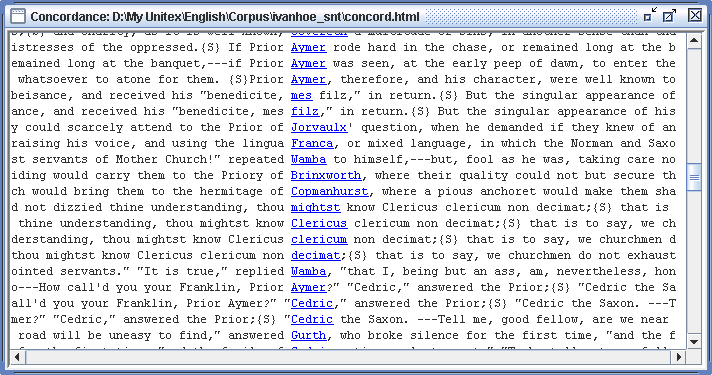
\includegraphics[width=15cm]{resources/img/fig4-1.png}
\caption{Résultat de la recherche du méta \texttt{<!DIC>}}
\end{center}
\end{figure}

\bigskip
\noindent Voici plusieurs exemples de motifs mélangeant les différentes sortes de contraintes:

\begin{itemize}
  \item \verb$<A~Hum:fs>$ : adjectif non humain au féminin singulier;
  \item \verb+<lire.V:P:F>+ : le verbe \textit{lire} au présent ou au futur;
  \item \verb$<suis,suivre.V>$ : le mot \textit{suis} en tant que forme conjuguée du verbe
  	  \textit{suivre}
  	  (par opposition à la forme du verbe \textit{être});
  \item \verb$<facteur.N~Hum>$ : toutes les entrées nominales ayant \textit{facteur} comme forme
  	  canonique et ne possédant pas le code sémantique \verb+Hum+;
  \item \verb$<!ADV>$ : tous les mots qui ne sont pas des adverbes;
  \item \verb$<!MOT>$ : tous les caractères, qui ne sont pas des lettres, sauf le séparateur de
  	  phrases
  	  (voir figure~\ref{fig-search-<!MOT>}). Ce masque ne reconnait pas le séparateur de phrase
  	  \verb+{S}+
  	  ni le tag \verb+{STOP}+.
  	  \index{\verb+{S}+}\index{Séparateur de phrase}\index{\verb+{STOP}+}
\end{itemize}

\bigskip
\begin{figure}[h]
\begin{center}
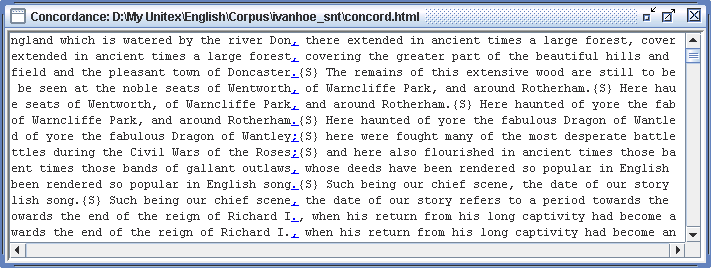
\includegraphics[width=15cm]{resources/img/fig4-2.png}
\caption{Résultat de la recherche du méta
\texttt{<!MOT>}\label{fig-search-<!MOT>}}
\end{center}
\end{figure}

\section{Concaténation}
\index{Concaténation d'expressions rationnelles}\index{\verb+.+}\index{Opérateur!concaténation}

On peut concaténer des expressions rationnelles de trois façons. La première consiste à
utiliser l’opérateur de concaténation représenté par le point. Ainsi, l’expression:

\begin{verbatim}
<DET>.<N>
\end{verbatim}

\noindent reconnaît un déterminant suivi par un nom. L’espace peut également servir à concaténer.
L’expression de l’exemple suivant:


\begin{verbatim}
le <A> chat
le<A>chat
\end{verbatim}

\noindent reconnaît l’unité lexicale \textit{le}, suivie d’un adjectif et de l’unité lexicale \textit{chat}.
Les parenthèses \index{Parenthèses} servent à délimiter une expression rationnelle.
Toutes les expressions suivantes sont équivalentes:


\begin{verbatim}
le <A> chat
(le <A>)chat
le.<A>chat
(le).<A> chat
(le.(<A>)) (chat)
\end{verbatim}

\section{Union}
\index{Union d'expressions rationnelles}\index{\verb$+$}
\index{Opérateur!disjonction}
L’union d’expressions rationnelles se fait en les séparant par le caractère \verb$+$.
L’expression:

\begin{verbatim}
(je+tu+il+elle+on+nous+vous+ils+elles) <V>
\end{verbatim}

\noindent
reconnaît un pronom suivi par un verbe. Si l’on veut rendre un élément facultatif dans
une expression, il suffit de faire l’union de cet élément avec le mot vide epsilon.
\index{\verb+<E>+} Exemples:

\bigskip
\noindent \verb$le(petit+<E>)chat$ reconnaît les séquences \textit{le chat}
et \textit{le petit chat}

\smallskip
\noindent \verb$(<E>+franco-)(anglais+belge)$ reconnaît \textit{anglais}, \textit{belge},
\textit{franco-anglais} et \textit{franco-belge}

\section{Kleene star}
\index{Kleene star}\index{\verb+*+}\index{Opérateur!Kleene star}
L’étoile de Kleene, représentée par le caractère \verb+*+,permet de reconnaître zéro, une ou
plusieurs occurrences d’une expression. L’étoile doit être placée à droite de l’élément concerné.
L’expression :


\begin{verbatim}
il fait très* froid
\end{verbatim}

\noindent reconnaît \textit{il fait froid}, \textit{il fait très froid},
\textit{il fait très très froid}, etc. L’étoile est prioritaire sur les
autres opérateurs. Il faut utiliser les parenthèses pour appliquer l’étoile à une expression
complexe. L’expression :


\begin{verbatim}
0,(0+1+2+3+4+5+6+7+8+9)*
\end{verbatim}

\noindent reconnaît un zéro, suivie d’une virgule et d’une suite éventuellement vide de chiffres.

\bigskip
\noindent ATTENTION : il est interdit de rechercher le mot vide avec une expression rationnelle.
Si l’on essaye de chercher \verb$(0+1+2+3+4+5+6+7+8+9)*$, le programme signalera une erreur
comme le montre la figure~\ref{fig-epsilon-error}.


\bigskip
\begin{figure}[h]
\begin{center}
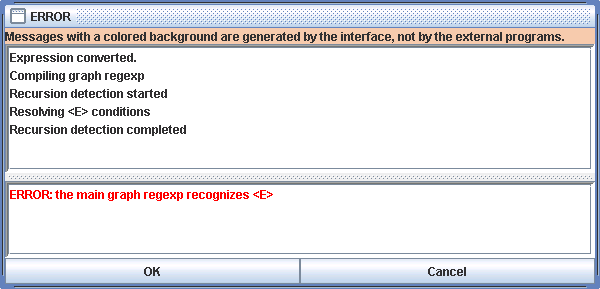
\includegraphics[width=14cm]{resources/img/fig4-3.png}
\caption{Erreur lors de la recherche d’une expression reconnaissant le mot vide \label{fig-epsilon-error}}
\end{center}
\end{figure}


\section{Filtres morphologiques}
\label{section-filters}
\index{Filtres morphologiques}

Il est possible d’appliquer des filtres morphologiques aux unités lexicales recherchées.
Pour cela, il faut faire suivre immédiatement l’unité lexicale considérée par un filtre entre
doubles angles:


\bigskip
\noindent
\textit{motif}\verb$<<$\textit{motif morphologique}\verb$>>$ \\


\bigskip\index{Expressions régulières}\index{POSIX}
\noindent Les filtres morphologiques s’expriment sous la forme d’expressions régulières au format
POSIX (voir \cite{TRE} pour une syntaxe détaillée). Voici quelques exemples de filtres élémentaires:




\begin{itemize}
  \item \verb$<<ss>>$: contient \verb$ss$
  \item \verb$<<^a>>$: commence par \verb$a$
  \item \verb+<<ez$>>+: finit par \verb$ez$
  \item \verb$<<a.s>>$: contient \verb$a$ suivi par un caractère quelconque, suivi par \verb$s$
  \item \verb$<<a.*s>>$: contient \verb$a$ suivi par un nombre de caractères quelconque, suivi par \verb$s$
  \item \verb$<<ss|tt>>$: contient \verb$ss$ ou \verb$tt$
  \item \verb$<<[aeiouy]>>$: contient une voyelle non accentuée
  \item \verb$<<[aeiouy]{3,5}>>$: contient une séquence de voyelles non accentuées, de longueur comprise entre 3 et 5
  \item \verb$<<es?>>$: contient \verb$e$ fsuivi par un \verb$s$ facultatif
  \item \verb$<<ss[^e]?>>$: contient \verb$ss$ suivi par un caractère qui n’est pas une voyelle \verb$e$
\end{itemize}

\bigskip
\noindent Il est possible de combiner ces filtres élémentaires pour former des filtres plus complexes:

\begin{itemize}
\item \verb+<<[ai]ble$>>+: finit par \verb$able$ ou \verb$ible$
\item \verb$<<^(anti|pro)-?>>$: commence par \verb$anti$ ou \verb$pro$, suivi par un tiret facultatif
  \item \verb+<<^([rst][aeiouy]){2,}$>>+: mot formé de 2 ou plus séquences commençant par un 
  	\verb$r$, \verb$s$ ou \verb$t$ suivi d’une voyelle non accentuée
  \item \verb!<<^([^l]|l[^e])>>!: ne commence pas par \verb$l$ ou alors la deuxième lettre n’est pas
un \verb$e$, c’est-à-dire n’importe quel mot sauf ceux qui commencent par \verb$le$.                                                                           De telles contraintes peuvent être exprimées plus simplement en utilisant des contextes
(voir~\ref{section-contexts}).
\end{itemize}

\noindent Par défaut, un filtre morphologique tout seul est considéré comme s’appliquant au méta
\verb$<TOKEN>$, c’est-à-dire à n’importe quelle unité lexicale sauf l’espace et le marqueur
\verb+{STOP}+.
En revanche, lorsqu’un filtre suit immédiatement un motif, il s’applique à ce qui est reconnu par
le motif. Voici quelques exemples de telles combinaisons:


\begin{itemize}
  \item \verb+<V:K><<i$>>+: participe passé finissant par \verb$i$
  \item \verb!<CDIC><<->>!: mot composé contenant un tiret
  \item \verb!<CDIC><< .* >>!: mot composé contenant deux espaces
  \item \verb!<A:fs><<^pro>>!: adjectif féminin singulier commençant par \verb$pro$
  \item \verb!<DET><<^([^u]|(u[^n])|(un.+))>>!: déterminant différent de \verb$un$
  \item \verb+<!DIC><<es$>>+: mot qui n’est pas dans le dictionnaire et qui se termine par \verb$es$
  \item \verb!<V:S:T><<uiss>>!: verbe au subjonctif passé ou présent, contenant \verb$uiss$
\end{itemize}

\noindent \index{Respect de la casse}NOTE : par défaut, les filtres morphologiques sont soumis aux
même variations de casse que les masques lexicaux. Ainsi, le filtre \verb$<<^é>>$ va reconnaître
tous les mots commençant par \texttt{é,}, mais également ceux qui commencent par \texttt{E} ou 
\texttt{É}. 
Pour forcer le respect exact de la casse du filtre, il faut ajouter \verb+_f_+ immédiatement après
celui-ci. Exemple : \verb+<A><<^é>>_f_+.



\section{Recherche}
\index{Configuration de la recherche}
\subsection{Configuration de la recherche}
Pour pouvoir rechercher une expression, il faut tout d’abord ouvrir un texte (voir chapitre
~\ref{chap-text}). Cliquez ensuite sur "Locate Pattern..." dans le menu "Text". La fenêtre de la
figure~\ref{fig-regexp-search-configuration} apparaît alors.

\bigskip
\begin{figure}[h]
\begin{center}
\includegraphics[width=8.8cm]{resources/img/fig4-4.png}
\caption{Fenêtre de recherche d’expressions\label{fig-regexp-search-configuration}}
\end{center}
\end{figure}

\noindent Le cadre "Locate Pattern" permet de choisir entre une expression rationnelle et une
grammaire. Cliquez sur "Regular expression".


\bigskip
\noindent Le cadre "Index" permet de sélectionner le mode de reconnaissance:

\bigskip
\index{Shortest matches}\index{Longest matches}\index{All matches}
\begin{itemize}
  \item "Shortest matches" : donne la priorité aux séquences les plus courtes
  	  %For instance, if your grammar can recognize the sequences \textit{a very hot chili} and 
  %\textit{very hot}, the first one will be discarded;
  \item "Longest matches" : donne la priorité aux séquences les plus longues. C’est le mode utilisé
  	  par défaut;
  \item "All matches" : donne toutes les séquences reconnues.
\end{itemize}

\bigskip
\noindent Le cadre "Search limitation" permet de limiter ou non la recherche à un certain nombre
d’occurrences. Par défaut, la recherche est limitée aux 200 premières occurrences.
\index{Occurrences!nombre}

\bigskip
\noindent Les options du cadre "Grammar outputs" ne concernent pas les expressions rationnelles.
Elles sont décrites à la section
~\ref{section-applying-graphs-to-text}. De même pour les options de l'onglet
"Advanced options" (voir section \ref{section-advanced-search-options}).

\bigskip
\noindent Dans le cadre "Search algorithm", on définit si l'on veut effectuer la recherche dans le
texte avec le programme \verb+Locate+ ou dans l'automate du texte avec le programme \verb+LocateTfst+.
Par défaut la recherche est effectuée avec le programme \verb+Locate+. Pour utiliser
\verb+LocateTfst+, il est utile de se référer à la section \ref{section-locate-tfst}.

\bigskip
\noindent Entrez une expression et cliquez sur "Search" pour lancer la recherche. Unitex va transformer
l’expression en une grammaire au format \verb+.grf+.
\index{Fichier!\verb+.grf+} Cette grammaire va ensuite être compilée en une grammaire au format
\verb+.fst2+\index{Fichier!\verb+.fst2+} qui sera utilisée par le programme de recherche.


\subsection{Affichage des résultats}
\label{section-display-occurrences}
Une fois la recherche terminée, la fenêtre de la figure~\ref{fig-search-results}
apparaît, indiquant le nombre d’occurrences trouvées, le nombre d’unités lexicales reconnues,
ainsi que le rapport entre ce nombre et le nombre total d’unités lexicales du texte.

\bigskip
\begin{figure}[h]
\begin{center}
\includegraphics[width=6.5cm]{resources/img/fig4-5.png}
\caption{Résultats de la recherche \label{fig-search-results}}
\end{center}
\end{figure}

\noindent Après avoir cliqué sur "OK", vous verrez apparaître la fenêtre de la
figure~\ref{fig-configuration-concordance} permettant de configurer l’affichage de la liste
des occurrences trouvées. Vous pouvez également faire apparaître cette fenêtre en cliquant sur
"Display Located Sequences..." dans le menu "Text".
On appelle \textit{concordance}\index{Concordance} la liste d’occurrences.


\bigskip
\begin{figure}[h]
\begin{center}
\includegraphics[width=11cm]{resources/img/fig4-6.png}
\caption{Configuration de l’affichage des occurrences trouvées\label{fig-configuration-concordance}}
\end{center}
\end{figure}

\bigskip
\noindent Le cadre "Modify text" offre la possibilité de remplacer les occurrences trouvées par les
sorties produites. Cette possibilité sera examinée au chapitre
~\ref{chap-advanced-grammars}.

\bigskip
\noindent Le cadre "Extract units" vous permet de construire un fichier texte avec toutes les phrases
contenant ou non des occurrences. Le bouton "Set File" vous permet de sélectionner le fichier
de sortie. Cliquez ensuite sur "Extract matching units" ou "Extract unmatching units" selon
que vous voulez extraire les phrases contenant les occurrences ou non.


\bigskip
\noindent Dans le cadre "Show Matching Sequences in Context", vous pouvez sélectionner la
longueur en caractères des contextes gauche et droit des occurrences qui seront affichées dans
la concordance. Si une occurrence a une longueur inférieure à la taille du contexte droit, la
ligne de concordance sera complétée avec le nombre de caractères nécessaire. Si une occurrence 
a une longueur supérieure à la taille du contexte droit, elle est affichée en entier.


\bigskip
\noindent NOTE: en thaï, la taille des contextes est mesurée en caractères affichables et non en
caractères réels. Cela permet de conserver l’alignement des lignes de concordance malgré la
présence de caractères diacritiques qui se combinent à d’autres lettres au lieu de s’afficher
comme des caractères normaux.


\index{Tri!des concordances}
\index{Contextes!concordance}
\bigskip
\noindent Vous pouvez sélectionner le mode de tri à appliquer dans la liste "Sort According to". Le
mode "Text Order" affiche les occurrences dans l’ordre où elles apparaissent dans le texte.
Les six autres modes permettent de trier en colonnes. Les trois zones d’une ligne sont le
contexte gauche, l’occurrence et le contexte droit. Les occurrences et les contextes droits
sont triés de gauche à droite. Les contextes gauches sont triés de droite à gauche. Le mode
utilisé par défaut est "Center, Left Col.". La concordance est produite sous la forme d’un
fichier HTML.\index{Fichier!HTML}

\bigskip
\noindent Lorsque les concordances atteignent plusieurs milliers d’occurrences, il est préférable
de les afficher avec un navigateur web (Firefox \cite{Firefox}, Netscape \cite{Netscape}, 
Internet Explorer, etc.).\index{Web browser}
\newline
Pour cela, cochez la case "Use a web browser to view the concordance" (voir figure
	~\ref{fig-configuration-concordance}). 
Cette option est activée par défaut lorsque le nombre d’occurrences est supérieur à 3000.
Pour définir le navigateur qui sera utilisé, cliquez sur "Preferences..." dans le menu "Info".
Cliquez sur l’onglet "Text Presentation" et sélectionnez le programme à utiliser dans le cadre
"Html Viewer" (voir figure~\ref{fig-browser-selection}).

\bigskip
\noindent \index{Cadre des concordance} Si vous choisissez d’ouvrir la concordance à l’intérieur
d’Unitex, vous verrez une fenêtre
comme celle de la figure \ref{fig-example-concordance}. 
L’option "Enable links" activée par défaut permet de considérer les occurrences comme des liens
hypertextes.
Ainsi, quand on clique sur une occurrence,
cela ouvre la fenêtre du texte et y sélectionne la séquence reconnue. De plus, si l’automate
du texte est construit et que cette fenêtre n’est pas réduite sous forme d’icône, l’automate
de la phrase contenant l’occurrence cliquée est chargé. Si l’on sélectionne l’option "Allow
concordance edition", on ne peut pas cliquer ainsi sur les occurrences, mais on peut éditer
la concordance comme du texte. Cela permet entre autres de s’y déplacer avec un curseur,
ce qui peut être pratique si l’on travaille sur une concordance avec de grands contextes.


\bigskip
\begin{figure}[h]
\begin{center}
\includegraphics[width=8cm]{resources/img/fig4-7.png}
\caption{Sélection d’un navigateur pour l’affichage des concordances\label{fig-browser-selection}}
\end{center}
\end{figure}

\bigskip
\begin{figure}[!p]
\begin{center}
\includegraphics[height=18cm]{resources/img/fig4-8.png}
\caption{Exemple de concordance\label{fig-example-concordance}}
\end{center}
\end{figure}

\clearpage
\subsection{Statistiques}
\label{section-statistics}
Si l'on sélectionne l'onglet ``Statistics'' dans le cadre ``Located sequences..'',
le panneau de la figure~\ref{fig-statistics} apparaît. Ce panneau permet d'effectuer des calculs
statistiques sur les séquences préalablement indexées.

\bigskip
\begin{figure}[!h]
\begin{center}
\includegraphics[width=11cm]{resources/img/fig4-9.png}
\caption{Panneau statistiques \label{fig-statistics}}
\end{center}
\end{figure}

\bigskip
\noindent Dans le panneau ``Mode'' il est possible de choisir le type de statistiques désiré:
\begin{itemize}
  \item collocates by frequency: montre les unités lexicales présentes dans le contexte de la
  	  séquence reconnu.
  \item collocates by z-score: le me mêmes informations avec, en plus (number of occurrences of the collocate in the match context and
  in the whole corpus, z-score of the collocate)
  \item contexts by frequency: montre les unités lexicales avec les contextes gauche et droit
  	  (voir au dessous). ``count'' est le nombre d'occurrences d'une séquence reconnue donnée
  	  (munie de contexte)
\end{itemize}

\bigskip
\noindent Dans le second panneau, on choisit la longueur des contextes gauche et droit à utiliser en
tokens sans espace.
NOTE: Cette notion de contexte n'a rien à voir avec celle utilisée dans les grammaires.


\bigskip
\noindent Dans le dernier panneau, on peut permettre ou non la variation de casse.
Si cette variation est permise, \verb$the$ et \verb$THE$ sont considérées comme la même unité
lexicale, et le résultat est la somme de ceux obtenus pour \verb$the$ et \verb$THE$.

\bigskip
\noindent Les figures suivantes montrent les statistiques calculées pour chaque mode pour la requête
\verb$<have>$ sur \verb$ivanhoe.snt$.


\bigskip
\begin{figure}[!h]
\begin{center}
\includegraphics[width=11cm]{resources/img/fig4-10.png}
\caption{contexte gauche+match+contexte droit+nombre d'occurrence\label{fig-statistics-mode0}}
\end{center}
\end{figure}

\begin{figure}[!h]
\begin{center}
\includegraphics[width=11cm]{resources/img/fig4-11.png}
\caption{collocate count\label{fig-statistics-mode1}}
\end{center}
\end{figure}

\begin{figure}[!h]
\begin{center}
\includegraphics[width=12cm]{resources/img/fig4-12.png}
\caption{collocate, count et d'autres informations\label{fig-statistics-mode2}}
\end{center}
\end{figure}

\chapter{Grammaires locales}
\label{chap-grammars}

Les grammaires locales sont un moyen puissant de représenter la plupart des phéno-
mènes linguistiques. La première section présentera le formalisme sur lesquel ces
grammaires reposent. Nous verrons ensuite comment construire et présenter des grammaires
avec Unitex.


\section{Formalisme des grammaires locales}
\index{Grammaires!formalisme}

\subsection{Grammaires algébriques}
Les grammaires Unitex sont des variantes des grammaires algébriques, également appelées
grammaires hors-contexte.\index{Grammaires!context-free} Une grammaire algébrique est constituée de
règles de réécriture. Voici une grammaire qui reconnaît n’importe quel nombre de caractères $a$:

\bigskip $S \rightarrow$ $aS$

$S \rightarrow$ \E

\bigskip
\noindent Les symboles figurant à gauche des règles sont appelés \textit{symboles
 non-terminaux}\index{Symboles!non-terminaux}\index{Symboles non-terminaux}                                                                                       car ils peuvent être réécrits. Les symboles qui ne peuvent pas être réécrits par des règles sont
 appelés \textit{symboles terminaux}\index{Symboles!terminaux}. Les membres droits des règles
sont des suites de symboles non-terminaux et terminaux. Le symbole epsilon noté \E ~
désigne le mot vide. Dans la grammaire ci-dessus, $S$ est un symbole non-terminal et
$a$ un terminal. $S$ peut se réécrire soit en un $a$ suivi d’un $S$,
soit en mot vide. L’opération de réécriture par l’application d’une règle est appelée
\textit{dérivation}.\index{Dérivation} On dit qu’une grammaire reconnaît un mot s’il existe
une suite de dérivations qui produit ce mot. Le non-terminal qui sert de point de départ
à la première dérivation est appelé \textit{axiome}.\index{Axiome}\index{Règles!réécriture}


\bigskip
\noindent La grammaire ci-dessus reconnaît ainsi le mot \textit{aa}, car on peut obtenir ce
mot depuis l’axiome $S$ en effectuant les dérivations suivantes:

\bigskip Dérivation 1: réécriture de l’axiome en $aS$

\underline{$S$} $\rightarrow aS$

\bigskip Dérivation 2: réécriture du $S$ du membre droit en $aS$

$S$ $\rightarrow a$\underline{$S$} $\rightarrow aaS$

\bigskip Dérivation 3: réécriture du $S$ to \E

$S$ $\rightarrow aS \rightarrow aa$\underline{$S$} $\rightarrow aa$

\bigskip
\noindent On appelle \textit{langage d’une grammaire} l’ensemble des mots reconnus par celle-ci.
%\textit{languagegenerated by the grammar}.
Les langages reconnus par les grammaires algébriques sont appelés \textit{Languages algébriques}
\index{Langages algébriques} ou \textit{Langages hors-contexte}\index{Langages hors-contexte}.


\subsection{Grammaires algébriques étendues}
\index{Grammaires!algébriques étendues}

   Les grammaires algébriques étendues sont des grammaires algébriques où les membres
droits des règles ne sont plus des suites de symboles mais des expressions rationnelles.
\index{Expressions rationnelles} Ainsi, la grammaire reconnaissant une suite quelconque de $a$
peut se réécrire en une grammaire étendue d’une seule règle:


\bigskip $S \rightarrow$ $a^{*}$

\bigskip
\noindent Ces grammaires, également appelées \textit{réseaux de transitions récursifs}
(\textit{RTN en Anglais})\index{Recursive Transition Networks}\index{RTN} ou
\textit{diagrammes de syntaxe}\index{Diagrammes de syntaxe}, se prêtent à une représentation graphique
conviviale. En effet, le membre droit d’une règle peut être représenté par un graphe dont le nom
est le membre gauche de la règle.


\bigskip
\noindent Toutefois, les grammaires Unitex ne sont pas exactement des grammaires algébriques
étendues, car elles intégrent la notion de \textit{transduction}.\index{Transduction} Cette notion,
empruntée aux automates à états finis, signifie qu’une grammaire peut produire des sorties.
Dans un souci de clarté, nous utiliserons malgré tout les termes grammaire ou graphe.
Quand une grammaire produira des sorties, nous utiliserons le terme \textit{transducteur},
\index{Transducteur} par extension de la définition d’un transducteur dans le domaine des automates
à états finis.\index{Automates!à états finis}


\section{Édition de graphes}
\label{section-editing-graphs}

\subsection{Création d'un graphe}
Pour pouvoir utiliser des graphes Intex dans Unitex, il faut les convertir en Unicode. Le
procédé de conversion est le même que pour les textes (voir section~\ref{fig-new-graph}).
Le symbole en forme de flèche est \textit{l'état initial} du graphe.\index{Etat!initial} Le symbole
composé d'un rond contenant un carré est  \textit{l'état final} du graphe.\index{Etat!final} La
grammaire reconnaît les séquences décrites par les chemins allant de l'état initial à l'état final


\begin{figure}[!h]
\begin{center}
\includegraphics[width=13cm]{resources/img/fig5-1.png}
\caption{Menu FSGraph}
\end{center}
\end{figure}

\begin{figure}[!h]
\begin{center}
\includegraphics[width=14.5cm]{resources/img/fig5-2.png}
\caption{Graphe vierge\label{fig-new-graph}}
\end{center}
\end{figure}

\bigskip
\noindent Pour créer une boîte, cliquez sur la fenêtre tout en appuyant sur la touche Ctrl. 
\index{Graphe!création d'une boîte} \index{Création d'une boîte}\index{Boîtes!création}
Vous verrez alors apparaître un carré bleu symbolisant la boîte vide créée (voir figure
~\ref{fig-box-creation}). Lors de la création d’une boîte, celle-ci est automatiquement sélectionnée.


\bigskip
\noindent Vous voyez donc le contenu de la boîte s’afficher dans la zone de texte située en
haut de la fenêtre. La boîte créée contient le symbole \verb+<E>+\index{\verb+<E>+} qui représente
le mot vide epsilon. Remplacez ce symbole par le texte \verb$I+you+he+she+it+we+they$ et validez en
appuyant sur la touche Entrée. Vous venez de créer une boîte contenant sept lignes (voir
	figure~\ref{fig-pronoun-box}).
En effet, le caractère \verb$+$ sert de séparateur.\index{\verb$+$} La boîte apparaît sous la
forme de lignes de texte rouge car elle n’est pour l’instant reliée à aucune autre.
On utilise souvent ce type de boîtes pour insérer des commentaires dans un graphe.
\index{Graphe!commentaires}\index{Commentaires!dans un graphe}

\bigskip
\noindent Si vous souhaitez ajouter un commentaire dans un graphe, vous devez créer une boîte qui
commence par \verb$/$. Le texte de la boîte est affiché en vert, et peut contenir des lignes vides.
La boîte ne peut avoir, ni de transition entrante, ni de transition sortante (voir
	figure~\ref{comment-box}).

\begin{figure}[!h]
\begin{center}
\includegraphics[width=14.5cm]{resources/img/fig5-3.png}
\caption{Création d’une boîte\label{fig-box-creation}}
\end{center}
\end{figure}

\begin{figure}[!h]
\begin{center}
\includegraphics[width=14.5cm]{resources/img/fig5-4.png}
\caption{Boîte contenant
\texttt{I+you+he+she+it+we+they}\label{fig-pronoun-box}}
\end{center}
\end{figure}

\begin{figure}[!h]
\begin{center}
\includegraphics[width=12.5cm]{resources/img/fig5-4b.png}
\caption{Boîte contenant un commentaire\label{comment-box}}
\end{center}
\end{figure}
%\clearpage


%\clearpage
\noindent Pour relier une boîte à une autre, il faut cliquer sur la boîte de départ, puis sur la
boîte de destination.\index{Graphe!connexion des boîtes}\index{Boîtes!connexion}
S’il y a déjà une transition entre les deux boîtes, celle-ci est enlevée. Il est possible
d’effectuer cette même opération en cliquant d’abord sur la boîte de destination, puis sur la boîte
de départ tout en pressant sur la touche Shift.
Dans notre exemple, une fois la boîte reliée à l’état initial et à l’état final du graphe,
on obtient le graphe de la figure~\ref{fig-pronoun-graph}:

\begin{figure}[!ht]
\begin{center}
\includegraphics[width=14.5cm]{resources/img/fig5-5.png}
\caption{Graphe reconnaissant des pronoms anglais\label{fig-pronoun-graph}}
\end{center}
\end{figure}

\bigskip
\noindent REMAQUE: si vous double-cliquez sur une boîte, vous relierez cette boîte à elle-même (voir
figure~\ref{fig-loop-box}). Pour annuler, double-cliquez une nouvelle fois sur la boîte.

\bigskip
\begin{figure}[!h]
\begin{center}
\includegraphics[width=4.5cm]{resources/img/fig5-6.png}
\caption{Boîte reliée à elle-même\label{fig-loop-box}}
\end{center}
\end{figure}

\noindent Cliquez sur "Save as..." dans le menu "FSGraph" pour enregistrer le graphe
\index{Graphe!enregistrement}. Par défaut, Unitex propose d'enregistrer le graphe dans le 
sous-répertpoire \verb+Graphs+ de votre répertoire personnel. Vous pouvez voir si le graphe a été
modifié après le dernièr enregistrement  en vérifiant si le titre du graphe contient le texte
\verb+(Unsaved)+.


%%%%%%%%%%%%%%%%%%%%%%%
\bigskip
\noindent Lorsque vous modifiez un graphe, vous pouvez faire apparaître, par un clic droit, un menu
contextuel vous permettant d'effectuer les opérations les plus usuelles.

\begin{itemize}
\item création d'une boîte
\item enregistrement, impression du graphe courant ou modifier les paramètres de la page
\item les menus habituels "Tools", "Format" et "Zoom" également accessibles dans le menu "FSGraph"
\end{itemize}
Si une ou plusieurs boîtes sont sélectionnées, les menus suivants deviennent accessibles, et
permettent d'effectuer plusieurs types d'opérations sur cet ensemble de boîtes. Sinon, ils sont
inutiles et donc désactivés. 
\begin{itemize}
\item entourer les boîtes sélectionnées avec des variables normales, des varaiables de sorties, des
contextes, ou des délimiteurs du mode morphologique. Ces opérations sont également réalisables avec
la barre d'outils de la fenêtre d'édition du graphe (voir section~\ref{toolbar-commands}). 
\item fusionner les boîtes sélectionnées
\item exporter les boîtes sélectionnées en tant que nouveau graphe
\end{itemize}
\bigskip
\begin{figure}[!h]
\begin{center}
\includegraphics[width=7.5cm]{resources/img/fig5-6b.png}
\caption{Menu contextuel\label{contextual-menu}}
\end{center}
\end{figure}

%%%%%%%%%%%%%%%%%%%%%%%%


\subsection{Sous-graphes}
\label{section-subgraphs}
\index{Graphe!appel à un sous-graphe}\index{\verb+:+}
Pour faire appel à un sous-graphe, il faut indiquer son nom dans une boîte en le faisant
précéder du caractère \verb+:+. Si vous entrez dans une boîte le texte suivant:

\bigskip
\verb$alpha+:beta+gamma+:E:\greek\delta.grf$

\bigskip
\noindent vous obtiendrez une boîte similaire à celle de la figure~\ref{fig-subgraph-call}:

\medskip
\begin{figure}[h]
\begin{center}
\includegraphics[width=6cm]{resources/img/fig5-7.png}
\caption{Graphe faisant appel aux sous-graphes \texttt{beta} et
\texttt{delta}\label{fig-subgraph-call}}
\end{center}
\end{figure}

\noindent Vous pouvez indiquer le nom complet du graphe
(\verb$E:\greek\delta.grf$) ou simplement le nom sans le chemin d’accès
 (\verb$beta$); dans ce cas, le sous-graphe est supposé se
trouver dans le même répertoire que le graphe qui y fait référence. Il est déconseillé d’utiliser 
des noms de graphes comportant des chemins absolus, car cela nuit à leur portabilité. Si
vous utilisez un nom de graphe absolu, comme c’est ici le cas pour \verb+E:\greek\delta.grf+
le compilateur de graphe émettra un avertissement (voir
figure~\ref{fig-warning-absolute-graph-name}).

\begin{figure}[!h]
\begin{center}
\includegraphics[width=14.5cm]{resources/img/fig5-8.png}
\caption{Avertissement pour un nom de graphe non portable\label{fig-warning-absolute-graph-name}}
\end{center}
\end{figure}


\bigskip
\noindent Pour les mêmes raisons de portabilité, il est déconseillé d’utiliser \verb+\+
ou \verb+/+ comme séparateur dans les noms de graphes. À la place, il vaut mieux utiliser
le caractère \verb+:+ qui joue le rôle de séparateur universel, valable quel que soit le système 
sous lequel vous travaillez. On peut d’ailleurs voir sur la figure
~\ref{fig-warning-absolute-graph-name}
que c’est ce séparateur qui est utilisé en interne par le compilateur de graphe
(\verb+E::greek:delta.grf+).

\bigskip
\noindent \textbf{Répertoire de dépôt}
\label{section-repository}

\bigskip
\noindent Lorsqu’on souhaite réutiliser une grammaire $X$ dans une grammaire $Y$, la méthode
usuelle est de recopier tous les graphes de $X$ dans le répertoire où se trouvent les graphes
de $Y$, ce qui pose deux problèmes :

\begin{itemize}
  \item le nombre de graphes dans le répertoire devient vite très important;
  \item deux graphes ne peuvent pas avoir le même nom.
\end{itemize}

\bigskip
\noindent Afin d’éviter cela, il est possible de stocker la grammaire $X$ dans un répertoire
particulier, appelé \textit{répertoire de dépôt}.\index{Répertoire de dépôt} Ce répertoire est
une sorte de bibliothèque dans laquelle on peut ranger des graphes, et faire ensuite appel
à ces graphes au moyen de \verb+::+  au lieu de \verb+:+. Pour utiliser ce mécanisme, il faut tout
d’abord définir le répertoire de dépôt dans le menu "Info>Preferences...>Directories" (voir figure
	\ref{directories}).
Choisissez votre répertoire dans le cadre "Graph repository". Le répertoire de dépôt est propre
à la langue de travail, vous n’êtes donc pas obligé d’utiliser le même répertoire pour plusieurs
langues.


\begin{figure}[!h]
\begin{center}
\includegraphics[width=8cm]{resources/img/fig5-10.png}
\caption{Configuration du répertoire de dépôt\label{directories}}
\end{center}
\end{figure}

\bigskip
\noindent Supposons que l’on ait une arborescence comme celle de la figure \ref{repository}. Si l’on
souhaite faire appel au graphe \verb+DET+ qui se trouve dans le sous-répertoire \verb+Johnson+, on
utilisera l’appel

% do not remove this line jump
\noindent \verb+::Det:Johnson:DET+
(voir figure \ref{repository-graph-call}\,\footnote{Dans un souci de clarté, les appels
à des graphes du répertoire de dépôt sont en marron au lieu de gris.}).


\bigskip
\begin{figure}[!h]
\begin{center}
\includegraphics[width=3.9cm]{resources/img/fig5-11.png}
\caption{Exemple de répertoire de dépôt\label{repository}}
\end{center}
\end{figure}

\begin{figure}[!h]
\begin{center}
\includegraphics[width=6.7cm]{resources/img/fig5-12.png}
\caption{Appel un graphe du répertoire de dépôt\label{repository-graph-call}}
\end{center}
\end{figure}

\bigskip
\noindent ASTUCE: si vous voulez éviter de mettre dans vos graphes un chemin compliqué
comme \verb+::Det:Johnson:DET+, vous pouvez créer un graphe nommé \verb+DET+ que vous placerez à la
racine du répertoire de dépôt \verb+D:\repository\DET.grf+). Ce graphe contiendra simplement
un appel au graphe \verb+::Det:Johnson:DET+. Vous pourrez alors mettre dans vos graphes un simple
appel à \verb+::DET+. Cela permet 1) de ne pas avoir de noms compliqués et 2) de pouvoir modifier
les graphes du répertoire de dépôt sans avoir à modifier tous vos graphes. En effet, il vous suffira
de mettre à jour le graphe situé à la racine du répertoire de dépôt.

%%%%%%%%%%%%%%%%%%%%%%%%%%%%%%

\begin{figure}[h!]
\begin{center}
\includegraphics[width=7cm]{resources/img/fig5-9.png}
\caption{Les sous-graphes manquants apparaissent en rouge}
\end{center}
\end{figure}

%%%%%%%%%%%%%%%%%%%%%%%%%%%%

\bigskip
\noindent Les appels à des sous-graphes sont représentés dans les boîtes par des lignes dont
l’arrière-plan est soit gris, soit marron dans le cas de sous-graphes à rechercher dans le 
répertoire de dépôt. Si le fichier \verb+.grf+ du sous-graphe n'est pas trouvé au chemin indiqué,
Unitex cherchera le fichier \verb+.fst2+ de même nom. Si Unitex ne trouve ni le fichier \verb+.grf+
ni le fichier \verb+.fst2+, l'appel au graphe manquant apparaît sur fond rouge. Sous Windows, vous
pouvez ouvrir un sous-graphe en cliquant sur la ligne grisée tout en appuyant sur la touche Alt.
Sous Linux, la combinaison <Alt+Click> est interceptée par le système\footnote{Si vous travaillez
sous KDE, désactivez <Alt+Click> dans kcontrol.}.
Pour ouvrir un sous-graphe, cliquez sur son nom en pressant simultanément les boutons gauche
et droit de la souris.

%%%%%%%%%%%%%%%%%%%%

\bigskip
\noindent La liste des graphes appelés par le graphe courant et celle des graphes qui appellent le
graphe courant peuvent être affichées en cliquant sur le second et troisième bouton du quatrième
groupe de boutons de la barre d'outils (voir figure~\ref{list-called-graphs} et
figure~\ref{fig-toolbar} à la section~\ref{toolbar-commands}).
Dans ces listes de sous-graphes:
\begin{itemize}
\item les sous-graphes directement appelés par le graphe courant apparaissent avec leur simple nom
	de fichier
\item les sous-graphes indirectement appelés par l'un des graphes appelés par le graphe courant
	apparaissent avec une flèche devant leurs nom
\item les sous-graphes qui apparaissent dans des graphes appelés par le graphe courant sans être
	connectés et donc non traités  ont leur nom en orange
\item les sous-graphes non trouvés (ni en .grf ni en .fst2) apparaissent en rouge.
\end{itemize}

\begin{figure}[!h]
\begin{center}
\includegraphics[width=15.2cm]{resources/img/fig5-12b.png}
\caption{Affichage de la liste de tous les graphes appelés\label{list-called-graphs}}
\end{center}
\end{figure}


%%%%%%%%%%%%%%%%%%

\subsection{Manipulation des boîtes}
\index{Sélection multiple}\index{Boîtes!sélection}

Vous pouvez sélectionner plusieurs boîtes au moyen de la souris. Pour cela, cliquez et
déplacez la souris sans relâcher le bouton. Lorsque vous relâcherez le bouton, toutes les
boîtes touchées par le rectangle de sélection seront sélectionnées et s’afficheront alors en
blanc sur fond bleu, figure \ref{multi-selection}.

\begin{figure}[!ht]
\begin{center}
\includegraphics[width=10cm]{resources/img/fig5-13.png}
\caption{Sélection de plusieurs boîtes\label{multi-selection}}
\end{center}
\end{figure}
\vspace{-0.3cm}
%%%%%%%%%%%%%%%
%\bigskip
\noindent Vous pouvez sélectionner plusieurs boîtes en maintenant les touches <CTRL> et <SHIFT> et
en cliquant sur chaque boîte à ajouter à la sélection. De cette manière, vous pouvez sélectionner
plusieurs boîtes sans avoir à sélectionner une zone complète.

\begin{figure}[!ht]
\begin{center}
\includegraphics[width=10cm]{resources/img/fig5-13b.png}
\caption{Sélection de boîtes éloignées\label{multi-selection2}}
\end{center}
\end{figure}
\vspace{-0.3cm}


%%%%%%%%%%%%%%
\bigskip
\noindent Lorsque des boîtes sont sélectionnées, vous pouvez les déplacer en cliquant et en déplaçant le curseur sans relâcher le bouton. Pour annuler la sélection, cliquez sur une zone vide
du graphe ; si vous cliquez sur une boîte, toutes les boîtes de la sélection seront reliées à
celle-ci.

\bigskip
\index{Sélection multiple!copier-coller}
\index{Copier}\index{Coller}
\noindent Vous pouvez effectuer un copier-coller sur plusieurs boîtes. Pour cela, sélectionnez-les
et appuyez sur <Ctrl+C> ou cliquez sur "Copy" dans le menu "Edit". Votre sélection multiple
est maintenant dans le presse-papiers d’Unitex. Vous pouvez alors coller cette sélection en
pressant <Ctrl+V> ou en cliquant sur "Paste" dans le menu "Edit".


\bigskip
\begin{figure}[!h]
\begin{center}
\includegraphics[width=13cm]{resources/img/fig5-14.png}
\caption{Copier-coller d’une sélection multiple}
\end{center}
\end{figure}

\noindent NOTE: Vous pouvez coller une sélection multiple dans des graphes différents de celui dont
elle est issue.

\bigskip
\index{Graphes!suppression de boîtes}\index{Boîtes!suppression}
\noindent Pour supprimer des boîtes, sélectionnez-les, effacez le texte qu'elles contiennent
(\textit{i.e.} le texte affiché dans le champ situé en haut de la fenêtre)
 et appuyez sur Enter. L'état initial et l'état final ne peuvent être supprimés.

\subsection{Sortie}
\index{Transducteurs}\index{\verb+/+}
Il est possible d’associer une sortie à une boîte. Pour cela, utilisez le caractère spécial
\verb+/+. Tous les caractères situés à droite de celui-ci seront considérés comme faisant partie de
la sortie. Ainsi, le texte \verb$one+two+three/number$ donne la boîte de la figure
~\ref{fig-exemple-transduction}. La sortie associée à une boîte est représentée en texte gras
sous celle-ci.\\


%\bigskip
\begin{figure}[h]
\begin{center}
\includegraphics[width=4.5cm]{resources/img/fig5-15.png}
\caption{Exemple de sortie\label{fig-exemple-transduction}}
\end{center}
\end{figure}


%%%%%%%%%%%%%%
\noindent \textbf{Poids}\\


Vous pouvez attribuer des poids à des boîtes d'un transducteur. Ainsi, lorsqu'une séquence est
reconnue par plusieurs chemins, seul celui de poids le plus élévé sera conservé.
Après un "Locate", la concordance, ne comportera qu'une seule fois la séquence reconnue avec la
sortie appropiée (figure~\ref{fig-weights-in-graphs}).

\bigskip
\begin{figure}[h!]
\begin{center}
\includegraphics[width=14.5cm]{resources/img/fig5-15b.png}
\caption{Poids dans les graphes \label{fig-weights-in-graphs}}
\end{center}
\end{figure}

%%%%%%%%%%%%%

\subsection{Utilisation des variables}
\label{section-using-variables}
\index{Graphe!variables}\index{Variables!dans les graphes}\index{\verb+$+}
\index{Transducteur!avec variables}

Il est possible de sélectionner des parties du texte reconnu par une grammaire au moyen
de variables. Pour associer une variable \verb+var1+ à une partie d’une grammaire, utilisez
les symboles spéciaux \verb+$var1(+ et \verb+$var1)+ pour définir respectivement le début et
la fin de la zone à stocker. Créez deux boîtes contenant l’une \verb+$var1(+ et l’autre
\verb+$var1)+. Ces boîtes ne doivent rien contenir d’autre que le nom de la variable précédé de
 \verb+$+ et suivi d’une parenthèse. Reliez ensuite ces boîtes à la zone de la grammaire voulue.
 Dans le graphe de la figure ~\ref{fig-using-variable} on reconnaît une séquence commençant par
 un nombre que l’on stocke dans une variable nommée \verb+var1+, suivi de \verb+dollar+ ou
 \verb+dollars+.

\bigskip
\begin{figure}[h]
\begin{center}
\includegraphics[width=13.5cm]{resources/img/fig5-16.png}
\caption{Utilisation d’une variable
\texttt{var1}\label{fig-using-variable}}
\end{center}
\end{figure}

\noindent Les noms de variables peuvent contenir des lettres latines non accentuées, minuscules
ou majuscules, ainsi que des chiffres et le caractère \verb+_+ (underscore).
\index{\verb+_+}\index{Noms de variables} Unitex fait la différence entre les lettres minuscules
et majuscules.\index{Underscore}

\bigskip
\noindent Quand une variable a ainsi été définie, on peut l’utiliser dans les sorties en encadrant
son nom avec le caractère \verb+$+.\index{\verb+$+} La grammaire de la figure
~\ref{fig-date-grammar} reconnaît une date formée d’un mois et d’une année,
 et produit en sortie la même date, mais dans l’ordre année-mois.

%Si l’on souhaite écrire en sortie le caractère \verb+$+.
%il faut le doubler, comme c’est le cas dans la figure ~\ref{fig-using-variable}.
\noindent Si vous voulez utiliser le caractère \verb+$+ en sortie d'une boîte, vous devez le
redoubler, comme le montre la figure~\ref{fig-using-variable}.

\bigskip
\begin{figure}[h]
\begin{center}
\includegraphics[width=14.5cm]{resources/img/fig5-17.png}
\caption{Inversion du mois et de l’année dans une date\label{fig-date-grammar}}
\end{center}
\end{figure}

%\noindent Si vous voulez utiliser le caractère \verb+$+ en sortie d'une boîte, vous devez le
%redoubler, comme le montre la figure~\ref{fig-using-variable}.

\bigskip
\noindent Par défaut \verb+Locate+ et \verb+LocateTfst+ considèrent que les variables non définies
sont vides. Vous pouvez modifier ce comportement (voir section \ref{section-advanced-search-options}).
De plus, il est  possible de savoir si une variable est définie ou non (voir section
\ref{section-variables}).

\subsection{Copie de listes}
\index{Copie de listes}
\index{Copie}\index{Coller}

Il peut être pratique d’effectuer un copier-coller d’une liste de mots ou d’expressions
depuis un éditeur de texte vers une boîte dans un graphe. Afin d’éviter de devoir copier
manuellement chaque terme, Unitex propose un mécanisme de copie de listes. Pour l’utili-
ser, sélectionnez votre liste dans votre éditeur de texte et copiez-la au moyen de <Ctrl+C> ou
de la fonction de copie intégrée à votre éditeur. Créez ensuite une boîte dans votre graphe,
et utilisez <Ctrl+V> ou la commande "Paste" du menu "Edit" pour la coller dans la boîte.
Vous verrez alors apparaître la fenêtre de la figure~\ref{fig-setting-contexts-for-multiple-copy}:

\bigskip
\begin{figure}[h]
\begin{center}
\includegraphics[width=7cm]{resources/img/fig5-18.png}
\caption{Sélection de contexte pour la copie d’une
liste\label{fig-setting-contexts-for-multiple-copy}}
\end{center}
\end{figure}
\index{Contextes!copie de liste}

\noindent Cette fenêtre vous permet de définir les contextes gauche et droit qui seront ajoutés
automatiquement à chaque terme de la liste. Par défaut, ces contextes sont vides. Si l’on applique
les contextes \verb+<+ et \verb+.V>+ à la liste suivante:

\bigskip
\textit{eat}

\textit{sleep}

\textit{drink}

\textit{play}

\textit{read}

\bigskip
\noindent on obtient la boîte de la figure~\ref{fig-multiple-copy}:

\bigskip
\begin{figure}[h]
\begin{center}
\includegraphics[width=6.7cm]{resources/img/fig5-19.png}
\caption{Boîte obtenue par copie d’une liste avec ajout de contextes\label{fig-multiple-copy}}
\end{center}
\end{figure}

\subsection{Symboles spéciaux}
\index{Symboles!spéciaux}
\noindent L’éditeur de graphes d’Unitex interprète de façon particulière les symboles suivants:

\bigskip
\verb," + : / < > # \,

\bigskip
\noindent Le tableau ~\ref{tab-special-symbols} résume la signification pour Unitex de ces symboles,
ainsi que la ou les façons de reconnaître ces caractères dans des textes.


\bigskip
\index{Meta-caractères}
\begin{table}[h]
\begin{center}
\begin{tabular}{|c|p{9cm}|c|}
\hline
\texttt{Caractère} & \texttt{Signification} & \texttt{Codage}
\\
\hline \verb$"$ & les guillemets délimitent des séquences qui ne doivent
ni être interprétées par Unitex, ni subir de variantes de casse
& \verb$\"$
\\
\hline
\verb$+$ & \verb$+$ sépare les différentes lignes boîtes& \verb$"+"$
\\
\hline
\verb$:$ & \verb$:$ sert à introduire à appel à un sous-graphe& \verb$":"$ or \verb$\:$
\\
\hline
\verb$/$ & \verb$/$ indique le début de la sortie d'une boîte& \verb$\/$
\\
\hline
\verb$<$ & \verb$<$ indique le début d'un motif ou d'un méta& \verb$"<"$ or \verb$\<$
\\
\hline
\verb$>$ & \verb$>$ indique la fin d'un motif ou d'un méta& \verb$">"$ or \verb$\>$
\\
\hline
\verb$#$ & \verb$#$ sert à interdire la présence de l'espace& \verb$"#"$
\\
\hline
\verb$\$ & \verb$\$ sert à déspécialiser la plupart des caractères spéciaux& \verb$\\$
\\
\hline
\end{tabular}
\caption{Codage des symboles spéciaux dans l’éditeur de graphes\label{tab-special-symbols}}
\end{center}
\end{table}

\subsection{Commandes de la barre d’icônes}
\index{Barre d'outils}
\label{toolbar-commands}

La barre d’icônes présente au-dessus des graphes contient des raccourcis vers certaines
commandes et permet de manipuler les boîtes d’un graphe en utilisant des "outils". Cette
barre d’icônes peut être déplacée en cliquant sur la zone "rugueuse". Elle peut même être
dissociée du graphe et apparaître alors comme une fenêtre séparée (voir figure~\ref{fig-toolbar}).
Dans ce cas, le fait de fermer cette fenêtre replace la barre d’icônes à sa position initiale.
Chaque graphe possède sa propre barre d’icônes.
\vspace{-0.1cm}
\begin{figure}[!ht]
\begin{center}
\includegraphics[width=15cm]{resources/img/fig5-20.png}
\caption{Barre d'outils\label{fig-toolbar}}
\end{center}
\end{figure}
\index{Copy}\index{Cut}\index{Paste}
\vspace{-0.3cm}

%\bigskip
\noindent Les deux premières icônes sont des raccourcis permettant de sauver et de compiler le
graphe. Les cinq suivantes correspondent aux opérations "Copier", "Couper", "Coller", "Redo" et
"Undo".\\

Les 6 icônes suivantes correspondent à des commandes d’édition des boîtes. La première,
en forme de flèche blanche, correspond au mode d’édition normal des boîtes. Les 5 autres
correspondent à des outils. Pour utiliser un outil, cliquez sur l’icône correspondante : le
curseur de la souris changera alors de forme et les clics de la souris seront alors interprétés
de façon particulière. Voici la description des outils, de gauche à droite:

\begin{itemize}
  \item création de boîtes: crée une boîte vide à l’endroit du clic;
  \item suppression de boîtes: supprime la boîte sur laquelle vous cliquez;
  \item relier des boîtes à une autre boîte: cet outil permet de sélectionner une ou plusieurs
boîtes, et de la ou les relier à une autre. À la différence du mode normal, la ou les
transitions qui vont être créées sont affichées pendant le déplacement du pointeur de
la souris;
  \item relier des boîtes à une autre boîte en sens inverse: cet outil effectue la même chose que
le précédent, mais en reliant en sens inverse les boîtes sélectionnées à la boîte cliquée;
  \item ouvrir un sous-graphe: ouvre un sous-graphe lorsque vous cliquez sur la ligne grisée
correspondante dans une boîte.
\end{itemize}

L'icône en forme de clé est un raccourci pour ouvrir la fenêtre des options d'affichage
du graphe. Les deux suivantes permettent de voir les listes de graphes en relation avec le
graphe courant:

\begin{itemize}
\item Le premier bouton affiche la liste des graphes appelés par le graphe courant
\item Le seconde bouton affiche la liste des graphes qui appellent le graphe courant
\end{itemize}

Le bouton muni de deux flèches vertes rafraîchit le graphe courant en chargeant sa dernière version.
Si un fichier \verb+.grf+ est modifié alors que le graphe qu'il contient est affiché dans
une fenêtre Unitex, une fenêtre pop up vous invitera à le recharger.

\bigskip
\noindent Le bouton portant l'icone d'une balance permet de comparer le graphe courant à un autre
graphe ou à une autre version du même graphe. Une nouvelle fenêtre est alors affichée (voir
	figure~\ref{Graph-DIFF}) qui contient les deux graphes avec des couleurs qui mettent en
relief les types de différences qui existent entre les deux graphes : insertion, suppression,
déplacement de boîtes et changement de contenu d'une boîte apparaissent respectivement en vert,
rouge, mauve et jaune.

\bigskip
\noindent 
\begin{figure}[!h]
\begin{center}
\includegraphics[width=15.6cm]{resources/img/DIFF.png}
\caption{DIFF\label{Graph-DIFF}}
\end{center}
\end{figure}
\bigskip
\noindent

Les six derniers boutons sont des raccourcis pour l'utilisation des variables, du mode morphologique
ou l'ajout de contextes autour d'une ou plusieurs boîtes sélectionnées. Ces boutons ne sont activés que si une  ou plusieurs boîtes sont sélectionnées:
\begin{itemize}
\item \textcolor{red}{()}  : variable normale	(voir section~\ref{section-using-variables})
\item \textcolor{blue}{()} : variable de sortie (voir section~\ref{section-output-variables})
\item \textcolor{magenta}{<>} : mode morphologique (voir section~\ref{section-morphological-mode})
\item \textcolor{green}{\$*} : contexte gauche (voir section~\ref{section-contexts})
\item \textcolor{green}{\$[} : contexte droit (voir section~\ref{section-contexts})
\item \textcolor{green}{\$![} : contexte droit négatif (voir section~\ref{section-contexts})
\end{itemize}

\bigskip
%\pagebreak


%%%%%%%%%%%%%%%%%%%

\section{Options de présentation}
\index{Graphe!présentation}

\subsection{Tri des lignes d’une boîte}
\index{Tri!des lignes d'une boîtes}\index{Boîtes!tri des lignes}
Vous pouvez trier le contenu d’une boîte en la sélectionnant et en cliquant sur "Sort Node
Label" dans le sous-menu "Tools" du menu "FSGraph". Ce tri ne fait pas appel au programme
\verb+SortTxt+. Il s’agit d’un tri basique qui trie les lignes de la boîte selon l’ordre des
caractères dans le codage Unicode.\index{Unicode}


\subsection{Zoom}
\index{Zoom}\index{Graphe!zoom}
Le sous-menu "Zoom" vous permet de choisir l’échelle à laquelle sera affiché le graphe.

\bigskip
\begin{figure}[h]
\begin{center}
\includegraphics[width=6.4cm]{resources/img/fig5-21.png}
\caption{Sous-menu Zoom}
\end{center}
\end{figure}

\noindent L’option "Fit in screen" étire ou rétrécit le graphe pour lui donner la taille de l’écran.
L’option "Fit in window" ajuste le graphe pour qu’il soit entièrement affiché dans la fenêtre.


\subsection{Antialiasing}
\index{Antialiasing}\index{Graphe!antialiasing}
L’antialiasing est un effet de rendu qui permet d’éviter l’effet de pixellisation.
\index{Pixellisation} Vous pouvez activer cet effet en cliquant sur "Antialiasing..."
dans le sous-menu "Format". La figure~\ref{fig-antialiasing} montre deux graphes affichés
normalement (graphe du haut) et avec antialiasing (graphe du bas).


\bigskip
\begin{figure}[!ht]
\begin{center}
\includegraphics[width=13.5cm]{resources/img/fig5-22.png}
\caption{Exemple d'antialiasing\label{fig-antialiasing}}
\end{center}
\end{figure}

\noindent Cet effet ralentit l’exécution d’Unitex. Nous vous conseillons de ne pas l’utiliser
si votre machine est peu puissante.


%\clearpage

\subsection{Alignement des boîtes}\index{Boîtes!alignement}
\index{Alignement des boîtes}\index{Graphe!alignement des boîtes}
Afin d’obtenir des graphes harmonieux, il est utile de pouvoir aligner les boîtes, aussi
bien horizontalement que verticalement. Pour cela, sélectionnez les boîtes à aligner et cli-
quez sur "Alignment..." dans le sous-menu "Format" du menu "FSGraph" ou appuyez sur
<Ctrl+M>. Vous voyez alors apparaître la fenêtre de la figure~\ref{fig-alignment-frame}.

\bigskip
\noindent Les possibilités d’alignement horizontal sont:
\begin{itemize}
  \item Top: les boîtes sont alignées sur la boîte la plus haute;
  \item Center: les boîtes sont toutes centrées sur un même axe;
  \item Bottom: les boîtes sont alignées sur la boîte la plus basse.
\end{itemize}

\begin{figure}[!h]
\begin{center}
\includegraphics[width=6.6cm]{resources/img/fig5-23.png}
\caption{Fenêtre d’alignement\label{fig-alignment-frame}}
\end{center}
\end{figure}

\noindent Les possibilités d’alignement vertical sont:
\begin{itemize}
  \item Left: les boîtes sont alignées sur la boîte la plus à gauche;
  \item Center: les boîtes sont toutes centrées sur un même axe;
  \item Right: les boîtes sont alignées sur la boîte la plus à droite.
\end{itemize}

\bigskip
\noindent La figure ~\ref{fig-vertical-left-alignment} montre un exemple 
d’alignement. Le groupe de boîtes situé à droite est une copie des boîtes
de gauche qui a été alignée verticalement à gauche.


\bigskip
\begin{figure}[!h]
\begin{center}
\includegraphics[width=11.5cm]{resources/img/fig5-24.png}
\caption{Exemple d’alignement vertical gauche\label{fig-vertical-left-alignment}}
\end{center}
\end{figure}

\bigskip
\noindent L’option "Use Grid" de la fenêtre d’alignement permet d’afficher une grille en
arrière-plan du graphe. Cela permet d’aligner approximativement les boîtes.
\index{Grille}

\bigskip
\begin{figure}[!h]
\begin{center}
\includegraphics[width=15cm]{resources/img/fig5-25.png}
\caption{Exemple d’utilisation d’une grille}
\end{center}
\end{figure}

\subsection{Présentation, polices et couleurs}
\label{section-display-fonts-colors}
\index{Graphe!options d'affichage, polices et couleurs}\index{Options!configuration}
\index{Couleurs!configuration}
Vous pouvez configurer l’aspect d’un graphe en appuyant sur <Ctrl+R> ou en cliquant
sur "Presentation..." dans le sous-menu "Format" du menu "FSGraph", ce qui provoque l’af-
fichage de la fenêtre de la figure~\ref{fig-graph-display-configuration}.

\begin{figure}[!h]
\begin{center}
\includegraphics[width=9cm]{resources/img/fig5-26.png}
\caption{Configuration de l’aspect d’un graphe\label{fig-graph-display-configuration}}
\end{center}
\end{figure}

\bigskip
\noindent Les paramètres de polices sont:
\begin{itemize}
  \item Input: police utilisée dans les boîtes, ainsi que dans la zone de texte où l’on édite le
contenu des boîtes;
\item Output: police utilisée pour afficher les sorties des boîtes.\index{Sorties d'un transducteur}
\end{itemize}

\bigskip
\noindent Les paramètres de couleur sont:
\begin{itemize}
  \item Background: couleur de fond;
  \item Foreground: couleur utilisée pour le texte et le dessin des boîtes;
  \item Auxiliary Nodes: couleur des boîtes faisant appel à des sous-graphes ;
  \item Selected Nodes: couleur utilisée pour dessiner les boîtes quand elles sont sélectionnées ;
  \item Comment Nodes: couleur utilisée pour dessiner les boîtes qui ne sont reliées à aucune autre.
\end{itemize}

\bigskip
\noindent Les autres paramètres sont:
\begin{itemize}
  \item Date: affichage de la date courante dans le coin inférieur gauche du graphe;
  \item File Name: affichage du nom du graphe dans le coin inférieur gauche du graphe;
  \item Pathname: affichage du nom du graphe avec son chemin complet dans le coin inférieur
gauche du graphe. Cette option n’a d’effet que si l’option "File Name" est sélectionnée;
  \item Frame: dessine un cadre autour du graphe;
  \item Right to Left: inverse le sens de lecture du graphe (voir exemple de la
  		  figure~\ref{fig-right-to-left-graph}).
\end{itemize}

\bigskip
\begin{figure}[!h]
\begin{center}
\includegraphics[width=14.5cm]{resources/img/fig5-27.png}
\caption{Graphe se lisant de droite à gauche\label{fig-right-to-left-graph}}
\end{center}
\end{figure}

\bigskip
\noindent Vous pouvez rétablir les paramètres par défaut en cliquant sur le bouton "Default".
Si vous cliquez sur le bouton "OK", seul le graphe courant sera modifié.\index{Preferences}
Pour modifier les préférences par défaut d’une langue, cliquez sur "Preferences..." dans le
menu "Info" et choisissez l’onglet "Graph Presentation".

%La fenêtre de configuration des préférences possède
%une option supplémentaire concernant l’antialiasing (voir figure
%order to modify the preferences for a language as a default, click on
%"Preferences..." in the "Info" menu and click on the "Graph configuration" button 
%in the "Language \& Presentation" tab.


\section{Les graphes en dehors d’Unitex}
\subsection{Inclusion d’un graphe dans un document}
\index{Graphe!inclure dans un document}\index{Inclure un graphe dans un document}
\index{Graphe!export en PNG}
Pour inclure un graphe dans un document, il faut en faire une image. Pour cela, une
première méthode consiste à sauver votre graphe en tant qu’image au format PNG. Pour
cela, allez dans le menu "FSGraph" et cliquez sur "Save as...". Choisissez ensuite le type de
fichier PNG. Vous obtiendrez ainsi une image prête à être intégrée dans un document ou
à être éditée avec un logiciel de retouche d’images. Afin de rendre l’image plus lisse, vous
pouvez activer l’antialiasing pour le graphe qui vous intéresse.


\bigskip
\noindent La seconde méthode consiste à faire une capture d’écran:

\bigskip
\noindent Sous Windows:

\bigskip
\noindent Appuyez ensuite sur la touche "Imprime écran" de votre clavier qui doit se trouver près
de la touche F12. Lancez le programme \verb+Paint+ dans le menu "Accessoires" de Windows. Appuyez sur 
<Ctrl+V>. \verb+Paint+ devrait vous dire que l’image contenue dans le presse-papiers
est trop grande et vous demander si vous voulez agrandir l’image. Cliquez sur "Oui". Vous
pouvez maintenant éditer l’image de l’écran. Sélectionnez la zone qui vous intéresse. Pour
cela, passez en mode sélection en cliquant sur le rectangle en pointillé qui se trouve dans
le coin supérieur gauche de la fenêtre. Vous pouvez maintenant sélectionner une zone de
l’image avec la souris. Une fois votre zone sélectionnée, appuyez sur <Ctrl+C>. Votre sélection
est maintenant dans le presse-papier, il ne vous reste plus qu’à aller dans votre document
et à appuyer sur <Ctrl+V> pour coller votre image.


\bigskip
\noindent Sous Linux:

\bigskip
\noindent Effectuez une capture d’écran (par exemple avec le programme \verb+xv+). Retaillez ensuite
votre image avec un éditeur graphique (par exemple \verb+TheGimp+), et collez votre image dans
votre document de la même façon que sous Windows.


\newpage
\bigskip
\noindent\textbf{Vector graphics}
\index{SVG export de graphe}
\index{Graphe!export SVG}

\bigskip
\noindent Si vous préférez vector graphics, vous pouvez enregistrer votre graphe en format
SVG, qui est utilisable avec des logiciels comme  Inkscape (\cite{Inkscape}).
Il permet d'obtenir des sorties PostScript utilisables dans des documents \LaTeX.

\subsection{Impression d’un graphe}
\index{Impression d’un graphe}\index{Impression!d’un graphe}

Vous pouvez imprimer un graphe en cliquant sur "Print..." dans le menu "FSGraph" ou
en appuyant sur <Ctrl+P>.


\bigskip
\noindent ATTENTION: vous devez vous assurer que le paramètre d’orientation de l’imprimante
(portrait ou paysage) correspond bien à l’orientation de votre graphe.


\bigskip
\noindent Vous pouvez définir vos préférences d’impression en cliquant sur "Page Setup" dans le
menu "FSGraph". Vous pouvez également imprimer tous les graphes qui sont ouverts en
cliquant sur "Print All...".




\chapter{Utilisation avancée des graphes}
\label{chap-advanced-grammars}
\section{Les types de graphes}
\index{Graphe!types de}\index{Types de graphes}
Unitex peut manipuler plusieurs types de graphes qui correspondent aux utilisations
suivantes : flexion automatique de dictionnaires, prétraitement des textes, normalisation
des automates de textes, graphes dictionnaires, recherche de motifs, levée d’ambiguïtés et
génération automatique de graphes. Ces différents types de graphes ne sont pas interprétés
de la même façon par Unitex. Certaines choses comme les sorties sont permises pour certains
types et interdites pour d’autres. De plus, les symboles spéciaux ne sont pas les mêmes en
fonction du type de graphe. Cette section présente donc chacun des types de graphes en
détaillant leurs particularités.


\subsection{Graphes de flexion}
\index{Transducteur!de flexion}\index{Flexion automatique}\index{Graphe!de flexion}
Un graphe de flexion décrit les variations morphologiques associées à une classe de
mots, en associant à chaque variante des codes flexionnels. Les chemins d’un tel graphe décrivent
les modifications à appliquer aux formes canoniques tandis que les sorties contiennent
les informations flexionnelles qui seront produites.


\bigskip
\begin{figure}[!h]
\begin{center}
\includegraphics[width=4.5cm]{resources/img/fig6-1.png}
\caption{Exemple de grammaire de flexion}
\end{center}
\end{figure}

\index{Opérateur!\verb+L+}
\index{Opérateur!\verb+R+}
\index{Opérateur!\verb+C+}
\index{Opérateur!\verb+D+}
\index{Opérateur!\verb+U+}
\index{Opérateur!\verb+P+}
\index{Opérateur!\verb+W+}
\index{\verb+L+}
\index{\verb+R+}
\index{\verb+C+}
\index{\verb+D+}
\index{\verb+U+}
\index{\verb+P+}
\index{\verb+W+}
\noindent Les chemins peuvent contenir des opérateurs et des lettres. Les opérateurs possibles
sont représentés par les caractères \verb+L+, \verb+R+, \verb+C+, \verb+D+, \verb+U+, \verb+P+ et
\verb+W+.
Les lettres qui ne sont pas des opérateurs sont des caractères. Le seul symbole spécial autorisé est
le mot vide \verb+<E>+.\index{\verb+<E>+} Il n’est pas possible de faire référence aux dictionnaires
dans un graphe de flexion. Il est cependant possible de
faire appel à des sous-graphes.

\bigskip
\noindent Les sorties sont concaténées pour produire une chaîne de caractères. Cette chaîne est
ensuite concaténée à la ligne de dictionnaire produite. Les sorties à variables n’ont pas de
sens dans un graphe de flexion.


\bigskip
\noindent Le contenu d’un graphe de flexion est manipulé sans aucune variante de casse: les lettres
minuscules restent minuscules, idem pour les majuscules. En outre, la liaison de deux boîtes
est strictement équivalente à la concaténation de leurs contenus munie de la concaténation
de leurs sorties (voir figure~\ref{fig-equivalent-inflection-paths}).\index{Respect!des
minuscules/majuscules}

\bigskip
\begin{figure}[!h]
\begin{center}
\includegraphics[width=5.5cm]{resources/img/fig6-2.png}
\caption{Deux chemins équivalents dans une grammaire de flexion\label{fig-equivalent-inflection-paths}}
\end{center}
\end{figure}

\bigskip
\noindent Les graphes de flexion doivent être compilés avant de pouvoir être utilisés par le pro-
gramme de flexion.


\bigskip
\noindent Pour plus de détails, voir section
\ref{section-automatic-inflection}.

\subsection{Graphes de prétraitement}
\index{Texte!prétraitement}\index{Grammaires!pour la reconnaissance de fin de phrase}
\index{Grammaires!normalisation!de formes non ambiguës}
Les graphes de prétraitement sont destinés à être appliqués aux textes avant que ceux-ci soient
découpés en unités lexicales. Ces graphes peuvent être utilisés pour insérer ou
remplacer des séquences dans les textes. Les deux utilisations usuelles de ces graphes sont
la normalisation de formes non ambiguës et le découpage en phrases.


\bigskip
\noindent L’interprétation de ces graphes dans Unitex est très proche de celle des graphes
syntaxiques utilisés pour la recherche de motifs. Les différences sont les suivantes:

\begin{itemize}
  \item on peut utiliser le symbole spécial \verb+<^>+ qui reconnaît un retour à la
  	  ligne;\index{\verb+<^>+}
  \item si l'on travaille en mode caractère par caractère, il est possible d'utiliser 
  	  le symbole spécial \verb+<L>+ qui reconnaît une lettre, telle que définie dans le fichier
  	  alphabet;\index{\verb+<L>+}
  \item il est impossible de faire référence aux dictionnaires;
  \item il est impossible d’utiliser les filtres morphologiques;
  \item il est impossible d’utiliser le mode morphologique;
  \item il est impossible d’utiliser des contextes.
\end{itemize}

Les figures~\ref{fig-example-sentence-splitting} (page \pageref{fig-example-sentence-splitting})
et~\ref{fig-normalization-grammar} (page \pageref{fig-normalization-grammar}) montrent des exemples
de graphes de prétraitement.


\subsection{Graphes de normalisation de l’automate du texte}
\label{section-normalizing-text-automataon}
\index{Automate!du texte}\index{Texte!automate du!normalisation}
\index{Grammaires!normalisation!de l'automate du texte}
\index{Normalisation!de l'automate du texte}
\index{Normalisation!de formes ambiguës}
Les graphes de normalisation de l’automate du texte permettent de normaliser des formes
ambiguës. En effet, ils peuvent décrire plusieurs étiquettes pour une même forme. Ces étiquettes
sont ensuite insérées dans l’automate du texte, explicitant ainsi les ambiguïtés. La
figure~\ref{fig-tfst-normalization-grammar} montre un extrait du graphe de normalisation utilisé
pour le français.

\bigskip
\begin{figure}[!h]
\begin{center}
\includegraphics[width=13.5cm]{resources/img/fig6-3.png}
\caption{Extrait du graphe de normalisation utilisé pour le
français\label{fig-tfst-normalization-grammar}}
\end{center}
\end{figure}

\noindent Les chemins décrivent les formes qui doivent être normalisées. Les variantes minuscules
et majuscules sont prises en compte selon le principe suivant : les lettres majuscules dans
le graphe ne reconnaissent que les lettres majuscules dans l’automate du texte ; les lettres
minuscules peuvent reconnaître les lettres minuscules et majuscules.\index{Respect de la casse}

\bigskip
\noindent Les sorties représentent les séquences d’étiquettes qui seront insérées dans l’automate
du texte. Ces étiquettes peuvent être des entrées de dictionnaires ou de simples chaînes
de caractères. Les étiquettes représentant des entrées de dictionnaire doivent respecter le
format des entrées d’un DELAF et être encadrées par les symboles
\verb+{+ et \verb+}+. Les sorties à variables n’ont pas de sens dans ce type de graphe.


\bigskip
\noindent Il est possible de faire appel à des sous-graphes. Il n’est pas possible de faire référence
aux dictionnaires pour décrire les formes à normaliser. L’unique symbole spécial reconnu
dans ce type de graphe est le mot vide \verb+<E>+.\index{\verb+<E>+}
Les graphes de normalisation de formes ambiguës doivent être compilés avant de pouvoir être
utilisés.


\subsection{Graphes syntaxiques}
\label{syntactic-graphs}\index{Graphe!syntaxique}\index{Grammaires!locales}
Les graphes syntaxiques, également appelés grammaires locales, permettent de décrire
des motifs syntaxiques qui pourront ensuite être recherchés dans des textes. De tous les
types de graphe, ceux-ci possèdent la plus grande puissance d’expressions, car ils permettent
de faire référence aux dictionnaires.\index{Référence aux informations dans les dictionnaires}
\index{Dictionnaire!référence aux informations du}

\bigskip
\noindent Les variantes minuscules/majuscules sont autorisées selon le principe décrit plus haut.
Il est toutefois possible de forcer le respect de la casse en encadrant une expression avec des
guillemets. L’emploi des guillemets permet également de forcer le respect des espacements.
En effet, Unitex considère, par défaut, qu’un espace est possible entre deux boîtes. Pour forcer
la présence d’un espace, il faut le mettre entre guillemets. Pour interdire la présence d’un
espace, il faut utiliser le symbole spécial \verb+#+.\index{\verb+#+}
\index{Respect!des minuscules/majuscules}\index{Casse!voir {Respect!des minuscules/majuscules}}
\index{Minuscules!voir {Respect!de minuscules/majuscules}}
\index{Majuscules!voir {Respect!de minuscules/majuscules}}
\index{Respect!des espaces}

\bigskip
\noindent Les graphes syntaxiques peuvent faire appel à des sous-graphes (voir section
~\ref{section-subgraphs}). Ils gèrent également les sorties, y compris les sorties à variables.
Les séquences produites sont interprétées comme des chaînes de caractères qui seront insérées
dans les concordances ou dans le texte si vous voulez modifier celui-ci (voir section
~\ref{section-modifying-text}).

\bigskip
\noindent Les graphes syntaxiques peuvent utiliser des contextes (voir section~\ref{section-contexts}).

\bigskip
\noindent Les graphes syntaxiques peuvent utiliser des filtres morphologiques (voir section
\ref{section-filters}).

\bigskip
\noindent Les graphes syntaxiques peuvent utiliser le mode morphologique (voir section
\ref{section-morphological-mode}).

\bigskip
\noindent Les symboles spéciaux supportés par les graphes syntaxiques sont les mêmes que ceux
utilisables dans les expressions rationnelles (voir section~\ref{section-special-symbols}).

\bigskip
\noindent Il n’est pas obligatoire de compiler les graphes syntaxiques avant de les utiliser pour la
recherche de motifs. Si un graphe n’est pas compilé, le système le compilera automatiquement.


\subsection{Grammaires ELAG}
\index{Grammaires!ELAG}\index{ELAG}

La syntaxe des grammaires de levée d’ambiguïtés est présentée à la section \ref{section-elag-grammars},
page \pageref{section-elag-grammars}.


\subsection{Graphes paramétrés}
\index{Graphe!paramétré}
Les graphes paramétrés sont des méta-graphes permettant de générer une famille de
graphes à partir d’une table de lexique-grammaire. Il est possible de construire des graphes
paramétrés pour n’importe quel type de graphe. La construction et l’utilisation des graphes
paramétrés seront développées dans le chapitre
~\ref{chap-lexicon-grammar}.

\section{Compilation d'une grammaire}
\label{section-graph-compilation}
\subsection{Compilation d'un graphe}
\index{Graphe!compilation}\index{Compilation!d'un graphe}
La compilation est l’opération qui permet de passer du format \verb+.grf+ à un format plus
facile à manipuler par les programmes d’Unitex. Pour compiler un graphe, vous devez
l’ouvrir, puis cliquer sur "Compile FST2" dans le sous-menu "Tools" du menu "FSGraph".
Unitex lance alors le programme \verb+Grf2Fst2+\index{\verb+Grf2Fst2+}\index{Programmes externes!\verb+Grf2Fst2+} dont vous pouvez suivre l’exécution dans une fenêtre
(voir figure~\ref{fig-compilation-frame}).

\bigskip
\begin{figure}[!h]
\begin{center}
\includegraphics[width=14.7cm]{resources/img/fig6-4.png}
\caption{Fenêtre de compilation\label{fig-compilation-frame}}
\end{center}
\end{figure}

\noindent Si le graphe fait appel à des sous-graphes, ceux-ci sont automatiquement compilés. Le
résultat est un fichier \verb+.fst2+ fichier\index{Fichier!\verb+.fst2+} qui rassemble tous les
graphes qui composent la grammaire. La grammaire est alors prête à être utilisée par les
différents programmes d’Unitex.


\subsection{Approximation par un transducteur fini}
\index{Graphe!approximation par transducteur fini}
\index{Approximation d'une grammaire par un transducteur fini}
\index{\verb+Flatten+}\index{Programmes externes!\verb+Flatten+}\label{flatten-section}
Le format FST2 conserve l’architecture en sous-graphes des grammaires, ce qui les différencie
des stricts transducteurs à états finis. Le programme \verb+Flatten+ permet de transformer
une grammaire FST2 en un transducteur à états finis quand cela est possible, et d’en
construire une approximation dans le cas contraire. Cette fonction permet ainsi d’obtenir des objets
plus simples à manipuler et sur lesquels peuvent s’appliquer tous les algorithmes classiques sur
les automates.


\bigskip
\noindent Pour compiler et transformer ainsi une grammaire, sélectionnez la commande "Compile
Flatten FST2" dans le sous-menu "Tools" du menu "FSGraph". La fenêtre de la figure~\ref{fig-flatten-configuration}
vous permet de configurer l’opération d’approximation.

\bigskip
\begin{figure}[!h]
\begin{center}
\includegraphics[width=10.4cm]{resources/img/fig6-5.png}
\caption{Configuration de l’approximation d’une grammaire\label{fig-flatten-configuration}}
\end{center}
\end{figure}

\noindent Le cadre "Flattening depth" permet de préciser le niveau d’imbrication des sous-graphes.
Cette valeur représente la profondeur maximale au-delà de laquelle les appels à des sous-
graphes ne seront plus remplacés par les sous-graphes eux-mêmes.


\bigskip
\noindent Le cadre "Expected result grammar format" permet de déterminer le comportement du
programme au-delà de la limite indiquée. Si vous sélectionnez l’option "Finite State Transducer",
les appels aux sous-graphes seront ignorés (remplacé par \verb+<E>+) au-delà de la profondeur
maximale. Cette option garantit ainsi l’obtention d’un transducteur à états finis, éventuellement
non équivalent à la grammaire de départ. En revanche, l’option "equivalent FST2" indique au
programme de laisser tels quels les appels aux sous-graphes au-delà de la profondeur limite.
Cette option garantit la stricte équivalence du résultat avec la grammaire d’origine, mais
ne produit pas forcément un transducteur à états finis. Cette option peut être utilisée pour
optimiser certaines grammaires.


\bigskip
\noindent Un message indique à la fin du processus d’approximation si le résultat est un transducteur
à états finis ou une grammaire FST2, et dans le cas d’un transducteur, s’il est équivalent
à la grammaire d’origine (voir figure~\ref{fig-flatten-result}).


\bigskip
\begin{figure}[!h]
\begin{center}
\includegraphics[width=14.7cm]{resources/img/fig6-6.png}
\caption{Résultat de l’approximation d’une grammaire\label{fig-flatten-result}}
\end{center}
\end{figure}


\subsection{Contraintes sur les grammaires}
\index{Grammaires!contraintes}\index{Contraintes sur les grammaires}
À l’exception des grammaires de flexion, une grammaire ne peut pas avoir de chemin
vide. Cela signifie que le graphe principal d’une grammaire ne doit pas pouvoir reconnaître
le mot vide, mais cela n’empêche pas un sous-graphe de cette grammaire de reconnaître
epsilon.


\bigskip
\noindent Il n’est pas possible d’associer une sortie à un appel à un sous-graphe. De telles sorties
sont ignorées par Unitex. Il faut donc utiliser une boîte vide située immédiatement à gauche
de l’appel au sous-graphe pour porter la sortie (voir figure~\ref{fig-subgraph-output}).
\index{Sortie d'un transducteur!associée à un appel de sous-graphe}

\bigskip
\begin{figure}[!h]
\begin{center}
\includegraphics[width=9.1cm]{resources/img/fig6-7.png}
\caption{Comment associer une sortie à un appel de sous-graphe\label{fig-subgraph-output}}
\end{center}
\end{figure}

\index{Boucles sans fin}
\noindent Les grammaires ne doivent pas non plus comporter de boucles infinies, car les programmes
d’Unitex ne pourraient jamais terminer l’exploration de telles grammaires.
%A void loop is a configuration that causes the \verb+Locate+ program to enter an infinite loop.
Ces boucles peuvent être dues à des transitions étiquetées par le mot vide epsilon ou à des
appels de sous-graphes récursifs.


\bigskip
\noindent Les boucles dues à des transitions par le mot vide peuvent avoir deux origines dont la
première est illustrée par la figure~\ref{fig-epsilon-output-loop}.
Ce type de boucle est dû au fait qu’une transition par le mot vide ne peut pas être éliminée
automatiquement par Unitex lorsqu’elle est munie d’une sortie. Ainsi, la transition par
le mot vide de la figure~\ref{fig-epsilon-output-loop} ne sera pas supprimée et provoquera une
boucle infinie.

\bigskip
\begin{figure}[!h]
\begin{center}
\includegraphics[width=6.2cm]{resources/img/fig6-8.png}
\caption{Boucle infinie due à une transition par le mot vide avec sortie\label{fig-epsilon-output-loop}}
\end{center}
\end{figure}

\bigskip
\noindent La seconde catégorie de boucle par epsilon concerne les appels à des sous-graphes pouvant
reconnaître le mot vide. Ce cas de figure est illustré par la
figure~\ref{fig-epsilon-subgraph-loop}: si le sous-graphe \verb+Adj+ reconnait epsilon, on a une
boucle infinie qu’Unitex ne peut pas éliminer.

\bigskip
\begin{figure}[!ht]
\begin{center}
\includegraphics[width=7.9cm]{resources/img/fig6-9.png}
\caption{Boucle infinie due à un appel à un sous-graphe reconnaissant epsilon
\label{fig-epsilon-subgraph-loop}}
\end{center}
\end{figure}

\begin{figure}[!ht]
\begin{center}
\includegraphics[width=15.5cm]{resources/img/fig6-10.png}
\caption{Boucle infinie causée par deux graphes s'appelant l'un l'autre
\label{fig-recursive-calls-loop}}
\end{center}
\end{figure}

\noindent La troisième possibilité de boucle infinie concerne les appels récursifs à des
sous-graphes. Considérons les graphes \verb+Det+ et \verb+DetCompose+ de la
figure~\ref{fig-recursive-calls-loop}.
 Chacun de ces graphes peut appeler l’autre \textit{sans rien lire dans le texte}. Le fait qu’aucun
 des deux graphes ne comporte d’étiquette entre l’état initial et l’appel à l’autre graphe est
 capital. En effet, s’il y avait au moins une étiquette différente d’epsilon entre le début du
 graphe \verb+Det+ et l’appel à \verb+DetCompose+, cela signifierait que les programmes d’Unitex
 explorant le graphe \verb+Det+ devraient lire le motif décrit par cette étiquette dans le texte
 avant d’appeler récursivement \verb+DetCompose+ Dans ce cas, les programmes ne pourraient boucler
 indéfiniment que s’ils rencontraient une infinité de fois le motif dans le texte, ce qui ne peut
 pas arriver.

\pagebreak
\subsection{Intervalle pour le nombre de répétitions}
\label{nb-repetitions}\index{Intervalle}\index{Boucle!nombre de répétitions}\index{Nombre de répétitions}\index{Répétition!nombre de}
\noindent Pour reconnaître des séquences de tokens dans laquelle un motif apparaît une fois, plusieurs fois
ou jamais, on peut associer un intervalle d'entiers à une boîte. Cela fixe les limites du nombre de fois
que le motif apparait. Le motif doit être décrit dans une boite unique.
Si on associe un intervalle  [m,M]  à une boîte contenant <A> (figure~\ref{intervals}), le chemin reconnaitra des séquences avec au moins $m$ adjectifs consécutifs et pas plus de $M$.

\begin{figure}[h!]
\begin{center}
\includegraphics[width=13.5cm]{resources/img/fig6-10a.png}
\caption{Utilisation d'un intervalle pour reconnaître plusieurs tokens consécutifs\label{intervals}}
\end{center}
\end{figure}

\noindent  On attache un intervalle en insérant \verb+$[m,M]$+ dans la sortie de la boite,
juste après le caractère ``/'', et selon les règles : 
\begin{itemize}
\item \verb+[m,M]+ = au moins $m$ motifs consécutifs et pas de plus de $M$
\item \verb+[,M]+ = de 0 à $M$  
\item \verb+[m,]+ = au moins $m$
\end{itemize}

\noindent La boite ne doit pas être connectée à elle-même par une boucle directe. Un intervalle est compatible avec 
une sortie au sens habituel. Par exemple, pour insérer sous la boite de la figure~\ref{intervals}
la sortie \verb+<ADJ position='antéposé'>+, saisissez  dans le champ
texte~: \verb+<A>/$[1,4]$/<ADJ position='antéposé'>+. 

\subsection{Détection d’erreurs}
\index{Détection d'erreur dans les graphes}\index{Graphe!détection d'erreur}
\index{Erreurs dans les graphes}
Pour éviter aux programmes de se bloquer ou de planter, Unitex effectue automatique-
ment une détection d’erreurs lors de la compilation des graphes. Le compilateur de graphes
vérifie que le graphe principal ne reconnaît pas le mot vide et recherche toutes les formes de
boucles infinies. Si une erreur est trouvée, un message d’erreur apparaît dans la fenêtre de
compilation. La figure ~\ref{fig-error-message} montre le message obtenu lorsqu’on tente de 
compiler le graphe \verb+Det+ de la figure~\ref{fig-recursive-calls-loop}.

\begin{figure}[!h]
\begin{center}
\includegraphics[width=15cm]{resources/img/fig6-11.png}
\caption{Message d’erreur obtenu en compilant le graphe
\texttt{Det}\label{fig-error-message}}
\end{center}
\end{figure}

\noindent Si vous avez lancé une recherche de motifs en sélectionnant un graphe au format 
\verb+.grf+ \index{Fichier!\verb+.grf+}, et qu’Unitex y décèle une erreur, l’opération
de recherche sera automatiquement interrompue.


\section{Contextes}
\index{Contexte!zone dans un graphe}\label{section-contexts}

Les graphes d’Unitex sont des grammaires algébriques. Elles sont également appelées
grammaires hors-contexte, car lorsque l’on souhaite reconnaître une séquence
 $A$, on ne tient pas compte du contexte dans lequel $A$ apparaît. Par exemple, il est 
 impossible de rechercher avec un graphe normal toutes les occurrences du mot \verb+president+, 
 sauf celles qui sont suivies par \verb+of the republic+.


\bigskip
\noindent Il est toutefois possible de tenir compte du contexte dans les graphes syntaxiques. Dans
ce cas, les graphes ne sont plus des grammaires algébriques, mais des grammaires contex-
tuelles qui n’ont pas les mêmes propriétés théoriques.
.

\subsection{Contextes droits}
\index{\verb+$[+}
\index{\verb+$]+}
On définit un contexte droit en délimitant une zone du graphe avec des boîtes contenant
\verb+$[+ and \verb+$]+, représentant respectivement les début et fin de contexte qui sont
représentés dans le graphe par des crochets verts. Le début et la fin d’un contexte doivent
apparaître dans le même graphe.


\bigskip
\begin{figure}[!h]
\begin{center}
\includegraphics[width=7.4cm]{resources/img/fig6-12.png}
\caption{Utilisation d’un contexte droit\label{fig-context1}}
\end{center}
\end{figure}

\bigskip
\noindent La figure~\ref{fig-context1} montre un exemple simple de contexte. Ce graphe
reconnaît tous les nombres qui sont suivis par l’euro, la livre ou le dollar, mais sans
que le symbole d’unité n’apparaisse dans les occurrences trouvées, c'est-à-dire dans
la concordance.

\bigskip
\noindent Les contextes s’interprètent de la façon suivante. Supposons que l’on rencontre un début
de contexte lors de l’application d’une grammaire à un texte, et notons $pos$ la position courante
dans le texte à cet instant. Le programme \verb$Locate$ va ensuite chercher à reconnaître
l’expression décrite dans le contexte. S’il échoue, il n’y aura pas de match. S’il réussit, c’est-
à-dire s’il peut atteindre la fin du contexte, le programme reviendra à la position $pos$ dans
le texte et continuera l’exploration de la grammaire à partir de la fin du contexte.

\bigskip
\noindent Les poids (section~\ref{Transducers}) dans les contextes droits sont ignorés.

\bigskip
\noindent On peut également définir des contextes droits négatifs, en utilisant
 \verb+$![+ comme début de contexte. La figure~\ref{fig-context2}
montre un graphe reconnaissant des nombres qui ne sont pas suivis par \verb+th+.
 La différence avec les contextes positifs est que lorsque \verb$Locate$ essaie de reconnaître
 l’expression décrite dans le contexte, le fait d’atteindre la fin du
 contexte est considéré comme un échec, car cela signifie que l’on a reconnu une séquence interdite.
 À l’inverse, si la fin de contexte ne peut être atteinte, le programme \verb$Locate$ reviendra à
 la position $pos$ dans le texte et continuera l’exploration de la grammaire à partir de la fin du
 contexte.

\begin{figure}[!h]
\begin{center}
\includegraphics[width=7.3cm]{resources/img/fig6-13.png}
\caption{Utilisation d’un contexte négatif\label{fig-context2}}
\end{center}
\end{figure}

\bigskip
\noindent Les contextes peuvent être placés n’importe où dans le graphe, y compris au début. La
figure~\ref{fig-context3} montre ainsi un graphe qui reconnaît un adjectif dans le contexte de
quelque
chose qui n’est pas un participe passé. Autrement dit, ce graphe reconnaît tous les adjectifs
qui ne sont pas ambigus avec des participes passés.

\begin{figure}[!h]
\begin{center}
\includegraphics[width=7.5cm]{resources/img/fig6-14.png}
\caption{Recherche d’un adjectif non ambigu avec un participe passé\label{fig-context3}}
\end{center}
\end{figure}

\bigskip
\noindent Dans les graphes tels que celui de la figure~\ref{fig-context3}, le contexte droit négatif
ne vérifie pas nécessairement le même nombre de tokens que la boite qui le suit. Par exemple, avant
que le graphe de la figure~\ref{too-also} ne reconnaisse \verb+too+, le contexte droit négatif
vérifie s'il apparait dans une expression telle que \verb+too early+ ou \verb+too many+.

\begin{figure}[!h]
\begin{center}
\includegraphics[width=7.5cm]{resources/img/fig-too-also.png}
\caption{Un contexte qui ne vérifie pas le même nombre de mots que la boite qui le suit\label{too-also}}
\end{center}
\end{figure}

\bigskip
\noindent On peut formuler des requêtes complexes avec les contextes droits négatifs. Ainsi, la figure
~\ref{fig-context4} montre un graphe qui reconnaît toutes les séquences de deux noms simples qui ne
sont pas ambiguës avec des mots composés. En effet, le motif \verb?<CDIC><<^([^ ]+ [^ ]+)$>>? 
reconnaît un mot composé contenant exactement un espace, et le motif \verb?<N><<^([^ ]+)$>>?
reconnaît un nom sans espace, c’est-à-dire un nom simple. Ainsi,
 dans la phrase \textit{Black cats should like the town hall}, ce graphe reconnaîtra
 \textit{Black cats}, mais pas \textit{town hall}, qui est un mot composé.

\bigskip
\begin{figure}[!h]
\begin{center}
\includegraphics[width=8.9cm]{resources/img/fig6-15.png}
\caption{Utilisation avancée des contextes\label{fig-context4}}
\end{center}
\end{figure}

\bigskip
\noindent Il est possible d’imbriquer des contextes. Par exemple, le graphe de la
figure~\ref{fig-context5}
reconnaît un nombre qui n’est pas suivi par un point, sauf si ce point est suivi par un nombre.
Ainsi, dans le texte \textit{5.0+7.=12}, ce graphe reconnaîtra \textit{5}, \textit{0} et
\textit{12}.

\bigskip
\begin{figure}[!h]
\begin{center}
\includegraphics[width=12cm]{resources/img/fig6-16.png}
\caption{Imbrication de contextes\label{fig-context5}}
\end{center}
\end{figure}

\bigskip
\noindent Les sorties qui se trouvent dans des boîtes à l’intérieur d’un contexte sont ignorées.
En revanche, il est possible d’utiliser une variable qui a été définie dans un contexte, comme
c’est le cas sur la figure ~\ref{fig-context6}). Si l’on applique ce graphe en mode MERGE au texte
\textit{the cat is white}, on obtient en sortie :

\bigskip
\texttt{the \textcolor{blue}{<pet name="cat" color="white"/>} is white}

\bigskip

\begin{figure}[!h]
\begin{center}
\includegraphics[width=12.2cm]{resources/img/fig6-17.png}
\caption{Variable définie dans un contexte\label{fig-context6}}
\end{center}
\end{figure}

\subsection{Contextes gauches}
\index{\verb+$*+}
Il est également possible de rechercher une expression $X$ si elle se trouve seulement après une 
expression $Y$. Évidemment, il était déjà possible de le faire avec une grammaire semblable à celle
de la figure \ref{fig-left-context1}. Cependant, avec ce type de grammaire, le contexte gauche est
inclus dans la séquence reconnue, comme le montre la figure~\ref{fig-left-context2}.

\begin{figure}[!ht]
\begin{center}
\includegraphics[width=7cm]{resources/img/fig6-17a.png}
\caption{Reconnaissance d'un nom précédé d'un déterminant numéral\label{fig-left-context1}}
\end{center}
\end{figure}

\begin{figure}[!ht]
\begin{center}
\includegraphics[width=14cm]{resources/img/fig6-17b.png}
\caption{Résultats de l'application de la grammaire de la figure
\ref{fig-left-context1}\label{fig-left-context2}}
\end{center}
\end{figure}

\bigskip
\noindent Pour éviter cela, on peut utiliser le symbole \verb+$*+ qui indique la fin du contexte
gauche de l'expression qu'on désire reconnaître. Ce symbole est représenté par une étoile verte
dans le graphe, comme le montre la figure~\ref{fig-left-context3}. L'effet d'un tel contexte est
d'utiliser une partie de la grammaire pour calculer la séquence reconnue, sans que cette partie ne figure dans le résultat (voir figure~\ref{fig-left-context4}).

\begin{figure}[!ht]
\begin{center}
\includegraphics[width=9cm]{resources/img/fig6-17c.png}
\caption{Reconnaissance d'un nom après un contexte gauche\label{fig-left-context3}}
\end{center}
\end{figure}

\begin{figure}[!ht]
\begin{center}
\includegraphics[width=14cm]{resources/img/fig6-17d.png}
\caption{Résultats de l'application de la grammaire de la figure
\ref{fig-left-context3}\label{fig-left-context4}}
\end{center}
\end{figure}

\clearpage
\noindent Toutes les sorties produites par un contexte gauche sont ignorées, comme on peut le voir dans la concordance de la figure \ref{fig-left-context6}, qui donne les résultats
obtenus avec la grammaire de la figure \ref{fig-left-context5}.

\begin{figure}[!ht]
\begin{center}
\includegraphics[width=9cm]{resources/img/fig6-17e.png}
\caption{Sorties ignorées dans un contexte gauche\label{fig-left-context5}}
\end{center}
\end{figure}

\begin{figure}[!ht]
\begin{center}
\includegraphics[width=15cm]{resources/img/fig6-17f.png}
\caption{Résultats de l'application de la grammaire de la figure
\ref{fig-left-context5}\label{fig-left-context6}}
\end{center}
\end{figure}

\bigskip
\noindent Toutefois, on peut mémoriser des informations avec des variables (voir section
\ref{section-variables}) et les utiliser en dehors du contexte gauche, comme le montrent la
grammaire de la figure~\ref{fig-left-context7} et son résultat dans la figure~\ref{fig-left-context8}.

\begin{figure}[!ht]
\begin{center}
\includegraphics[width=10cm]{resources/img/fig6-17g.png}
\caption{Utilisation d'une variable dans un contexte gauche\label{fig-left-context7}}
\end{center}
\end{figure}

\begin{figure}[!ht]
\begin{center}
\includegraphics[width=15cm]{resources/img/fig6-17h.png}
\caption{Résultats de l'application de la grammaire de la figure
\ref{fig-left-context7}\label{fig-left-context8}}
\end{center}
\end{figure}

\bigskip
\noindent On peut invoquer dans une grammaire un graphe qui contient des contextes gauches,
mais cela nécessite d'être vigilant. Au moment où le contexte gauche est exclu de la séquence reconnue,
toutes les séquences qui avaient été reconnues par des graphes appelants en sont exclues également,
car la séquence qui sera finalement reconnue devra être contiguë. Les sorties correspondant aux
séquences exclues sont ignorées elles aussi.

\bigskip
\noindent Ainsi, avec des contextes gauche et droit, on peut faire une distinction entre les motifs
utilisés pour reconnaître des points du texte, et la délimitation des séquences à extraire dans les 
résultats. Par exemple, la grammaire de la figure \ref{fig-left-context9} cherche des
expressions comme \verb$the animal's$, mais extrait seulement les noms, comme on peut le voir
figure \ref{fig-left-context10}.

\begin{figure}[!ht]
\begin{center}
\includegraphics[width=10cm]{resources/img/fig6-17i.png}
\caption{Une grammaire avec des contextes gauche et droit\label{fig-left-context9}}
\end{center}
\end{figure}

\begin{figure}[!ht]
\begin{center}
\includegraphics[width=15cm]{resources/img/fig6-17j.png}
\caption{Résultats de l'application de la grammaire de la figure
\ref{fig-left-context9}\label{fig-left-context10}}
\end{center}
\end{figure}

\bigskip
\noindent Les poids (section~\ref{Transducers}) fonctionnent normalement dans les contextes gauches.

\clearpage

\section{Le mode morphologique}
\label{section-morphological-mode}
\index{Mode morphologique}
\subsection{Pourquoi ?}
Comme Unitex fonctionne sur une version "tokenisée" du texte, il n'est pas possible de
faire des requêtes qui entrent à l'intérieur des "tokens", sauf avec les filtres morphologiques
(voir section \ref{section-filters}), comme le montre la figure
\ref{fig-morpho1}.

\begin{figure}[!ht]
\begin{center}
\includegraphics[width=8cm]{resources/img/fig6-17k.png}
\caption{Reconnaissance d'éléments morphologiques\label{fig-morpho1}}
\end{center}
\end{figure}

\bigskip
\noindent Cependant, les filtres morphologiques ne permettent pas n'importe quelle requête, puisqu'ils ne
peuvent pas faire référence aux informations contenues dans les dictionnaires. Ainsi, il est impossible de formuler de cette 
manière une requête comme ``\textit{un mot constitué du préfixe} \verb$un$ \textit{suivi d'un adjectif en} \verb+able+''.

\bigskip
\noindent Pour surmonter cette difficulté, nous introduisons un mode morphologique dans le programme
\verb$Locate$. Il consiste à délimiter une partie de votre  grammaire avec les 
symboles \verb+$<+ et \verb+$>+.\index{\verb+$<+}\index{\verb+$>+}
Dans cette zone, les données sont reconnues lettre par lettre, comme le montre la figure
\ref{fig-morpho2}.

\begin{figure}[!ht]
\begin{center}
\includegraphics[width=11cm]{resources/img/fig6-17l.png}
\caption{Exemple de zone morphologique dans la grammaire\label{fig-morpho2}}
\end{center}
\end{figure}

\subsection{Les règles}
Dans ce mode, le contenu du graphe n'est pas interprété de manière habituelle.
\begin{enumerate}
\item Il n'y a pas d'espace entre les boîtes. Ainsi, si on désire reconnaître un espace,
	on doit le rendre explicite avec \verb+" "+ (un espace entre guillemets).

\item On peut toujours utiliser des sous-graphes, mais la fin de la zone morphologique
	doit se trouver dans le même graphe que son début.

\item On peut utiliser des masques lexicaux qui nécessitent la consultation d'un dictionnaire
--- comme \verb+<DIC>+ , \verb+<be>+ ou \verb+<N:ms>+, qui font référence aux informations contenues dans un dictionnaire ---, du moment qu'il a été préalablement déclaré comme dictionnaire
du mode morphologique (voir section~\ref{dic-mode-morpho}). 
   
\item On peut utiliser des masques lexicaux qui nécessitent la consultation d'un graphe-dictionnaire
(section~\ref{section-dictionary-graphs}), du moment que le nom du graphe-dictionnaire contient l'option \verb+b+.
Cependant, cette possibilité ne fonctionne que pour les formes reconnues dans le texte par le graphe-dictionnaire
pendant l'application initiale des dictionnaires (section~\ref{section-applying-dictionaries}),
et non pour les formes qui n'apparaissent dans le texte que comme des parties de tokens.
   
\item On peut utiliser des filtres morphologiques (section~\ref{section-filters}). Cependant, les filtres
           morphologiques employés seuls ou sur \verb+<TOKEN>+
	ne s'appliqueront seulement qu'au caractère courant. Par 
	conséquent, les filtres comme \verb+<<[1-9][0-9]>>+ qui sont conçus pour reconnaître plus d'un
	caractère ne reconnaîtront jamais rien. En fait, dans le mode morphologique, 
	les filtres morphologiques ne sont utiles que pour exprimer des négations
	comme \verb+<<[^aeiouy]>>+ (n'importe quel caractère qui n'est pas une voyelle). 
   
\item Les contextes gauches et droits au sens de la section~\ref{section-contexts} sont interdits.

\item On peut utiliser des sorties.
   
\item \verb+<LETTER>+ reconnaît n'importe quelle lettre définie dans le fichier alphabet  (l'ancien masque <MOT> reste toujours valable).
	\index{\verb+<MOT>+}\index{\verb+<LETTER>+}

\item \verb+<LOWER>+ reconnaît n'importe quelle minuscule définie dans le fichier alphabet (l'ancien masque <MIN> reste toujours valable).\index{\verb+<MIN>+}\index{\verb+<LOWER>+}

\item \verb+<UPPER>+ reconnaît n'importe quelle majuscule définie dans le fichier alphabet (l'ancien masque <MAJ> reste toujours valable).\index{\verb+<MAJ>+}\index{\verb+<UPPER>+}

\item \verb+<DIC>+ reconnaît n'importe quel mot présent dans un dictionnaire du mode
	 morphologique\index{\verb+<DIC>+}, mais les méta-symboles \verb+#+, \verb+<FIRST>+, \verb+<PRE>+, \verb+<NB>+,
 	 \verb+<SDIC>+ et\verb+<CDIC>+ sont interdits.\index{\verb+#+}\index{\verb+<FIRST>+}\index{\verb+<PRE>+}\index{\verb+<NB>+} \index{\verb+<TOKEN>+}\index{\verb+<SDIC>+} \index{\verb+<CDIC>+}

\item Si on atteint la fin de la zone sans être à la fin du token, la reconnaissance échoue.
	Par exemple, si le texte contient \verb+enabled+, on ne peut pas reconnaître seulement
	\verb+enable+.
\end{enumerate}

\subsection{Dictionnaires du mode morphologique}
\index{Dictionnaire!du mode morphologique}
\label{dic-mode-morpho}
Dans le mode morphologique, on peut faire des requêtes qui utilisent les dictionnaires.
Par exemple,  la grammaire de la figure \ref{fig-morpho3} cherche les mots constitués du préfixe \verb+un+ suivi d'un adjectif.

\begin{figure}[!ht]
\begin{center}
\includegraphics[width=11cm]{resources/img/fig6-17m.png}
\caption{Reconnaissance des mots constitués de \textit{un} et d'un adjectif en 
\textit{able}\label{fig-morpho3}}
\end{center}
\end{figure}

\begin{figure}[!ht]
\begin{center}
\includegraphics[width=11cm]{resources/img/fig6-17n.png}
\caption{Déclaration des dictionnaires du mode morphologique\label{fig-morpho4}}
\end{center}
\end{figure}

\bigskip
\noindent Pour pouvoir reconnaître le mot 
\verb+unaware+ avec cette grammaire, le système doit savoir que \verb+aware+ est un adjectif. 
Le masque lexical \verb+<A>+ nécessite la consultation d'un dictionnaire. Mais
\verb+aware+ peut ne pas être présent dans le texte, de sorte qu'on ne peut pas compter
sur les dictionnaires du texte\footnote{Les dictionnaires du texte sont compilés pendant l'application
initiale des dictionnaires (section~\ref{section-applying-dictionaries}), non pas pendant la recherche
de motifs.}.
C'est la raison pour laquelle on doit définir une liste de
dictionnaires à consulter en mode morphologique.
Pour ce faire, on va dans ``Info>Preferences>Morphological-mode dictionaries''
(figure~\ref{fig-morpho4}).
On peut définir autant de dictionnaires du mode morphologique qu'on veut, mais ils doivent
être au format \verb+.bin+. Ceci fait, on peut appliquer la grammaire.
Pour spécifier qu'un graphe-dictionnaire doit être consulté lorsqu'on est en mode morphologique,
on utilise l'option \verb+b+ ou \verb+z+ (section~\ref{section-dictionary-graphs}, Exporter les entrées produites
comme dictionnaire du mode morphologique).

\subsection{Variables de dictionnaire}
\index{Variable!de dictionnaire}
\index{Variable!morphologique}
\label{dictionary-variables}
On peut affecter à des variables des informations issues des dictionnaires du mode morphologique.
Ces variables sont appelées variables de dictionnaire ou variables morphologiques.
L'initialisation d'une variable de ce type doit être associée à une boite contenant un motif
qui fait référence à des informations contenues dans un dictionnaire du mode morphologique,
à l'exception du motif \verb+<DIC>+. On met \verb+$xxx$+ en sortie de la boîte, où \verb+xxx+ est un nom
correct de variable (cf. section~\ref{section-using-variables}). Ceci affecte à une  variable dénommée \verb+xxx+
l'entrée de dictionaire reconnue par le motif.
Dans la suite des chemins qui passent par la boite, on peut obtenir la forme fléchie, la forme canonique et les codes fournis par l'entrée avec
\verb+$xxx.INFLECTED$+, \verb+$xxx.LEMMA$+ et \verb+$xxx.CODE$+, comme le montre la figure
\ref{fig-morpho5}.
On peut également utiliser les motifs suivants:

\begin{itemize}
\item \verb+$xxx.CODE.GRAM$+: fournit seulement le premier code grammatical,
	censé être la catégorie grammaticale
  
\item \verb+$xxx.CODE.SEM$+: fournit tous les autres codes,
	séparés par des \verb$+$, s'il en existe
  
\item \verb+$xxx.CODE.FLEX$+: fournit tous les codes flexionnels
  séparés par des \verb$:$, s'il en existe

\item \verb+$xxx.CODE.ATTR=yyy$+ renvoie la valeur d'une paire attribut-valeur contenue dans les codes sémantiques, c'est-à-dire la valeur \verb+zzz+ de l'attribut \verb+yyy+ s'il y figure un  code sémantique de la forme \verb+yyy=zzz+.

\end{itemize}
	
\noindent Les variables de dictionnaire peuvent être utilisées en dehors du mode morphologique,
comme sur la figure \ref{fig-morpho7}. On peut effectuer des tests sur ces variables comme expliqué
dans la section \ref{section-variables}.

\begin{figure}[!ht]
\begin{center}
\includegraphics[width=16cm]{resources/img/fig6-17o.png}
\caption{Utilisation d'une variable de dictionnaire\label{fig-morpho5}}
\end{center}
\end{figure}

\begin{figure}[!ht]
\begin{center}
\includegraphics[width=15cm]{resources/img/fig6-17p.png}
\caption{Résultats de la  grammaire de la figure \ref{fig-morpho5} appliquée en mode in MERGE
\label{fig-morpho6}}
\end{center}
\end{figure}

\begin{figure}[!ht]
\begin{center}
\includegraphics[width=15.5cm]{resources/img/fig6-17q.png}
\caption{Utilisation d'une variable de dictionnaire en mode normal\label{fig-morpho7}}
\end{center}
\end{figure}


\bigskip
\noindent \textbf{Variables de dictionnaire dans LocateTfst}

\noindent Pour les grammaires appliquées avec \verb+LocateTfst+ (cf. section~\ref{section-locate-tfst}), on dispose d'une possibilité
supplémentaire. 
En dehors du mode morphologique, on peut mémoriser dans une variable de dictionnaire
une étiquette lexicale contenue dans l'automate du texte.
Il suffit pour cela d'associer à la boîte une sortie de la forme \verb+$:abc$+ où \verb+abc+
est le nom de la variable.
On peut ensuite l'utiliser comme variable de dictionnaire habituelle, de la façon décrite ci-dessus~:
on peut obtenir la forme fléchie, la forme canonique et les codes donnés dans l'entrée, sa
catégorie grammaticale, ses codes sémantiques, ses codes flexionnels et la valeur
 \verb+zzz+ de l'attribut \verb+yyy+ s'il y figure un  code sémantique de la forme \verb+yyy=zzz+.


\section{Exploration des chemins d’une grammaire}
\index{Exploration des chemins d’une grammaire}

Il est possible de générer les chemins reconnus par une grammaire, par exemple pour
vérifier qu’elle engendre correctement les formes attendues. Pour cela, ouvrez le graphe
principal de votre grammaire et assurez-vous que la fenêtre du graphe est bien la fenêtre active
(la fenêtre active possède une barre de titre bleu, tandis que les fenêtres inactives ont une
barre de titre grise). Allez ensuite dans le menu "FSGraph", puis dans le sous-menu "Tools",
et cliquez sur "Explore graph paths". La fenêtre de la figure 
~\ref{fig-explore-graph-paths} apparaît alors.


\begin{figure}[!h]
\begin{center}
\includegraphics[width=10.4cm]{resources/img/fig6-18.png}
\caption{Exploration des chemins d’une grammaire\label{fig-explore-graph-paths}}
\end{center}
\end{figure}

\bigskip
\noindent Le cadre supérieur contient le nom du graphe principal de la grammaire à explorer.
Les options suivantes concernent la gestion des sorties de la grammaire ainsi que le mode
d’exploration:


\begin{itemize}
  \item "Ignore outputs": les sorties sont ignorées;
  \item "Separate inputs and outputs": les sorties sont affichées groupées après les entrées
  (\verb$ a b c / A B C$);
  \item "Merge inputs and outputs": chaque sortie est affichée immédiatement après l’entrée 
  	  qui lui correspond
  (\verb$a/A b/B c/C$).
  \item "Only paths": les appels aux sous-graphes sont explorés récursivement;
  \item "Do not explore subgraphs recursively": les appels aux sous-graphes sont affichés sans
être explorés récursivement.
\end{itemize}

\noindent Si l’option "Maximum number of sequences" est cochée, le nombre spécifié sera le nombre
maximum de chemins générés. Si l’option n’est pas sélectionnée, tous les chemins seront générés.


\bigskip
\noindent Voici ce que l’on obtient pour le graphe de la figure ~\ref{fig-glace} 
 avec les paramètres par défaut (ignorer les sorties, limite = 100 chemins) :


\bigskip
\noindent
\texttt{<NB> <boule> de glace \`a la pistache}

\noindent
\texttt{<NB> <boule> de glace \`a la fraise}

\noindent
\texttt{<NB> <boule> de glace \`a la vanille}

\noindent
\texttt{<NB> <boule> de glace vanille}

\noindent
\texttt{<NB> <boule> de glace fraise}

\noindent
\texttt{<NB> <boule> de glace pistache}

\noindent
\texttt{<NB> <boule> de pistache}

\noindent
\texttt{<NB> <boule> de fraise}

\noindent
\texttt{<NB> <boule> de vanille}

\noindent
\texttt{glace \`a la pistache}

\noindent
\texttt{glace \`a la fraise}

\noindent
\texttt{glace \`a la vanille}

\noindent
\texttt{glace vanille}

\noindent
\texttt{glace fraise}

\noindent
\texttt{glace pistache}

\begin{figure}[!h]
\begin{center}
\includegraphics[width=10.9cm]{resources/img/fig6-19.png}
\caption{Exemple de graphe \label{fig-glace}}
\end{center}
\end{figure}




\section{Collection de graphes}
\index{Collection de graphes}

Il peut arriver que l’on souhaite appliquer plusieurs grammaires situées dans un même
répertoire. Pour cela, il est possible de construire automatiquement une grammaire à partir
d’une arborescence de fichiers. Supposons par exemple que l’on ait l’arborescence suivante:


\begin{itemize}
  \item \textit{Dicos}:
  \begin{itemize}
    \item \textit{Banque}:
    \begin{itemize}
      \item \texttt{carte.grf}
    \end{itemize}
    \item \textit{Nourriture}:
    \begin{itemize}
      \item \texttt{eau.grf}
      \item \texttt{pain.grf}
    \end{itemize}
    \item \texttt{truc.grf}
  \end{itemize}
\end{itemize}

\noindent Si l’on veut rassembler toutes ces grammaires en une seule, on peut le faire avec la
commande "Build Graph Collection" dans le sous-menu "FSGraph > Tools". On configure cette
opération au moyen de la fenêtre de la figure
~\ref{fig-build-graph-collection}.

\begin{figure}[!h]
\begin{center}
\includegraphics[width=9cm]{resources/img/fig6-20.png}
\caption{Construction d’une collection de graphes\label{fig-build-graph-collection}}
\end{center}
\end{figure}

\noindent Dans le champ "Source directory", sélectionnez le répertoire racine que vous voulez
explorer (dans notre exemple, le répertoire \textit{Dicos}).  Dans le champ "Resulting GRF grammar",
indiquez le nom de la grammaire produite.


\bigskip
\noindent ATTENTION : ne placez pas la grammaire de sortie dans l’arborescence que vous
voulez explorer, car dans ce cas, le programme va chercher à lire et à écrire simultanément
dans ce fichier, ce qui provoquera un plantage.


\bigskip
\noindent Lorsque vous cliquerez sur "OK", le programme recopiera les graphes dans le répertoire de
la grammaire de sortie, et créera des sous-graphes correspondant aux différents
sous-répertoires, comme on peut le voir sur la figure~\ref{fig-graph-collection}, qui montre
le graphe de sortie engendré pour notre exemple.


\bigskip
\noindent On peut constater qu’une boîte contient les appels à des
sous-graphes correspondant à des sous-répertoires (ici les répertoires \textit{Banque}
et \textit{Nourriture}), et que l’autre boîte fait appel à tous les graphes qui se trouvaient
dans le répertoire (ici le graphe \texttt{truc.grf}).

\begin{figure}[!h]
\begin{center}
\includegraphics[width=11cm]{resources/img/fig6-21.png}
\caption{Graphe principal d’une collection de graphes\label{fig-graph-collection}}
\end{center}
\end{figure}



\section{Règles d’application des transducteurs}
\label{section-applying-transducers-rules}
\index{Transducteur!règles d'application}\index{Règles!pour l'application des transducteurs}
Cette section décrit les règles d’application des transducteurs lors des opérations de pré-
traitement et de recherche de motifs. Les graphes de flexion et de normalisation de formes
ambiguës ne sont pas concernés par ce qui suit.


\subsection{Insertion à gauche du motif reconnu}
\index{MERGE}\index{REPLACE}
Lorsqu’un transducteur est appliqué en mode REPLACE, les sorties remplacent les séquences lues dans le texte. 
%When a box in a transducer has no output, it is processed as if it had an \verb+<E>+ output.
En mode MERGE, les sorties sont insérées à gauche des séquences reconnues. Considérons le
transducteur de la figure~\ref{fig-transducer-example}
. 

\begin{figure}[!h]
\begin{center}
\includegraphics[width=7.2cm]{resources/img/fig6-22.png}
\caption{Exemple de transducteur\label{fig-transducer-example}}
\end{center}
\end{figure}

\bigskip
\noindent 
%Look at the transducer in Figure~\ref{fig-transducer-example}.
\noindent Si l’on applique ce transducteur au roman  \textit{Ivanhoe} by Sir Walter Scott
en mode MERGE, on obtient la concordance de la figure~\ref{fig-transducer-example-concordance} 


\begin{figure}[!h]
\begin{center}
\includegraphics[width=14.4cm]{resources/img/fig6-23.png}
\caption{Concordance obtenue en mode MERGE avec le transducteur de la figure
~\ref{fig-transducer-example}\label{fig-transducer-example-concordance}}
\end{center}
\end{figure}

\subsection{Application en avançant}
Pendant les opérations de prétraitement, le texte est modifié au fur et à mesure qu’il
est parcouru. Afin d’éviter le risque de boucler indéfiniment, il ne faut pas que les 
séquences produites par un transducteur puissent être ré-analysées par celui-ci. Pour cette
raison, quand une séquence a été introduite dans le texte, l’application du transducteur se
poursuit après cette séquence.
Cette règle ne concerne que les transducteurs de prétraitement, car lors de l’application
de graphes syntaxiques, les sorties ne modifient pas le texte parcouru, mais un fichier de
concordances distinct du texte.


\subsection{Priorité à gauche}
\label{section-priorite-gauche}
\index{Priorité!à la séquence de gauche} \index{Chevauchement d'occurrences}
Lors de l’application d’une grammaire locale, les occurrences qui se chevauchent sont
toutes indexées.
Nous considérons, ici, de vrai chevauchements d'occurrence comme \verb+abc+ et \verb+bcd+, et
pas d'occurrences imbriquées comme \verb+abc+ et \verb+bc+.
Lors de la construction de la concordance, toutes ces occurrences sont présentées
(voir figure~\ref{fig-overlappping-occurrences}).

\begin{figure}[!h]
\begin{center}
\includegraphics[width=13cm]{resources/img/fig6-24.png}
\caption{Occurrences se chevauchant dans une concordance\label{fig-overlappping-occurrences}}
\end{center}
\end{figure}

\noindent En revanche, si vous modifiez le texte au lieu de construire une concordance, il est
nécessaire de choisir parmi ces occurrences lesquelles seront prises en compte. Pour cela, Unitex
 applique la règle de priorité suivante : la séquence la plus à gauche l’emporte.

\bigskip
\noindent Si l’on applique cette règle aux trois occurrences de la concordance précédente, l’occurrence \textcolor{blue}{\texttt{[in ancient]}} est concurrente avec 
\textcolor{blue}{\texttt{[ancient times]}}. C’est donc la première qui
est retenue car c’est l’occurrence la plus à gauche, et \textcolor{blue}{\texttt{[ancient times]}} est
éliminée. L’occurrence suivante  \textcolor{blue}{\texttt{[times a]}} n’est donc plus en conflit avec 
\textcolor{blue}{\texttt{[ancient times]}} et peut donc apparaître dans le résultat:

\begin{center}
\texttt{...Don, there extended \textcolor{blue}{[in ancient] [times a]} large forest...}
\end{center}

\noindent La règle de priorité à gauche s’applique uniquement lorsque le texte est modifié, soit lors
du prétraitement, soit après l’application d’un graphe syntaxique (voir section 
~\ref{section-modifying-text}).

\subsection{Priorité aux séquences les plus longues}
\index{Priorité!à la séquence la plus longue}
Lors de l’application d’un graphe syntaxique, il est possible de choisir si la priorité doit
être donnée aux séquences les plus courtes ou les plus longues, ou si toutes les séquences
doivent être retenues. Lors des opérations de prétraitement, la priorité est toujours donnée
aux séquences les plus longues.


\subsection{Sorties à variables}
\label{section-variables}
\index{Variable!dans un graphe}\index{Sortie d'un transducteur!avec variable}
Comme nous l’avons vu à la section~\ref{section-using-variables}, il est possible d’utiliser
des variables d'entrée pour mémoriser le texte qui a été analysé par une grammaire. Ces variables
peuvent être utilisées dans les graphes de prétraitement et dans les graphes syntaxiques.


\bigskip
\noindent Vous devez donner des noms aux variables que vous utilisez. Ces noms peuvent contenir
les lettres comprises entre \verb+A+ et \verb+Z+, non accentuées minuscules ou majuscules, 
des chiffres et le caractère \verb+_+ (underscore).\index{Underscore}

\bigskip
\noindent Pour définir le début (ou la fin) de la zone à stocker dans une variable d'entrée, vous devez créer
une boîte contenant le nom de la variable encadré par les caractères
\verb-$- et \verb-(- (\verb-$- et \verb-)- pour la fin d’une variable). Pour utiliser une variable
dans une sortie, vous devez faire précéder et suivre son nom du caractère \verb-$- (voir figure~\ref{fig-variable-definition}).

\bigskip
\noindent Les variables sont globales. Cela signifie que vous pouvez définir une variable dans un
graphe et l’appeler dans un autre, comme l’illustrent les graphes de la figure
~\ref{fig-variable-definition}.

\begin{figure}[!p]
\begin{center}
\includegraphics[width=12cm]{resources/img/fig6-25.png}
\caption{Définition d’une variable d'entrée dans un sous-graphe\label{fig-variable-definition}}
\end{center}
\end{figure}

\bigskip
\noindent Si on applique le graphe \verb+TitleName+ en mode MERGE au texte
\textit{Ivanhoe}, on obtient la concordance de la figure ~\ref{fig6-14}.

\begin{figure}[!p]
\begin{center}
\includegraphics[width=13.5cm]{resources/img/fig6-26.png}
\caption{Concordance obtenue par l’application du graphe \texttt{TitleName}\label{fig6-14}}
\end{center}
\end{figure}

\index{Déplacements de groupes de mots}
\bigskip
\noindent Les sorties à variables peuvent être utilisées pour déplacer des groupes de mots. En effet,
l’application d’un transducteur en mode REPLACE n’écrit dans le texte que les séquences
produites par des sorties. Pour intervertir deux groupes de mots, il suffit donc de les stocker
dans des variables et de produire une sortie avec ces variables dans l’ordre souhaité. Ainsi,
le transducteur de la figure
~\ref{fig-swapping-words} appliqué en mode REPLACE au texte \textit{Ivanhoe}
donne la concordance de la figure~\ref{fig-no-space-problem}.

\begin{figure}[!ht]
\begin{center}
\includegraphics[width=11.3cm]{resources/img/fig6-27.png}
\caption{Interversion de mots grâce à deux variables d'entrée\label{fig-swapping-words}}
\end{center}
\end{figure}

\begin{figure}[!ht]
\begin{center}
\includegraphics[width=13.4cm]{resources/img/fig6-28.png}
\caption{Résultat de l’application du transducteur de la figure~\ref{fig-swapping-words}\label{fig-no-space-problem}}
\end{center}
\end{figure}

\bigskip
\noindent Si le début ou la fin d’une variable est mal défini (fin d’une variable avant son début,
absence du début ou de la fin d’une variable), celle-ci sera ignorée lors des sorties.
Consultez la section \ref{section-advanced-search-options} pour d'autres options affectant
le traitement d'erreurs concernant les variables.

\bigskip
\noindent Il n’y a aucune limite au nombre de variables utilisables.

\bigskip
\noindent    Les variables d'entrées peuvent être imbriquées, et même se chevaucher comme le montre la
figure~\ref{fig-overlapping-variables}.

\begin{figure}[!ht]
\begin{center}
\includegraphics[width=15cm]{resources/img/fig6-29.png}
\caption{Chevauchement de variables d'entrée\label{fig-overlapping-variables}}
\end{center}
\end{figure}

%\clearpage


\newpage

\section{Variables de sortie}
\label{section-output-variables}
\index{Variable!de sortie}
Les variables d'entrée sont déclarées avec \verb+$xxx(+ et \verb+$xxx)+ mémorisent des portions du
texte d'entrée. 
Il est aussi possible de mémoriser des parties des sorties produites par une grammaire.
Cela met en jeu des variables de sortie.
Ces variables sont déclarées avec \verb+$|xxx(+ et \verb+$|xxx)+.
Elles apparaissent en bleu (voir figure \ref{fig-output-variables}).
Remarquons qu'au moment où une variable de sortie est initialisée,
les séquences de sortie du transducteur ne sont pas émises dans la sortie correspondant à l'occurrence courante,
elles sont seulement mémorisées dans la variable de sortie créée par cette opération.
Par ailleurs, les sorties sont calculées en premier~: si une sortie contient une chaine comme 
\verb+$A.LEMMA$+, la variable de sortie ne contiendra pas cette chaîne mais le lemme associé à
la variable \verb+A+. En outre, les variables de sortie mémorisent seulement des sorties
effectivement produites par votre grammaire. Ainsi, même si vous travaillez en mode MERGE, les
variables de sortie ne mémorisent jamais le texte d'entrée.

\noindent Cet exemple de grammaire appliquée en mode MERGE au texte \textit{Ivanhoe} produit la
concordance visible sur la figure \ref{fig-output-variables-concord}. 
Ainsi, vous pouvez voir que les sorties \verb+ADJ+ et \verb+NOUN+ n'ont pas été insérées à gauche du texte d'entrée comme on aurait pu s'y attendre.

\begin{figure}[!ht]
\begin{center}
\includegraphics[width=8cm]{resources/img/fig6-17r.png}
\caption{Variables de sortie\label{fig-output-variables}}
\end{center}
\end{figure}

\begin{figure}[!ht]
\begin{center}
\includegraphics[width=15cm]{resources/img/fig6-17s.png}
\caption{Concordances obtenues avec la grammaire de la figure ~\ref{fig-output-variables}\label{fig-output-variables-concord}}
\end{center}
\end{figure}


\section{Opérations sur les variables}
\label{section-ops-on-variables}
\subsection{Tests sur les variables}
\index{Tests sur les variables}\index{Variable!interrogation}

\noindent Il est possible de tester si une variable est définie ou non, afin d'interrompre la
reconnaissance courante si la condition n'est pas vérifiée. Ceci se fait en insérant la  séquence
\verb+$xxx.SET$+ dans la sortie d'une boîte. Ainsi, si une variable dénommée \verb+xxx+ a été définie,
cette séquence est ignorée et la reconnaissance continue, sinon, la reconnaissance s'arrête
et le programme repart en arrière. Ceci fonctionne sur les variables d'entrée, les variables de
sortie et les variables de dictionnaire. De façon similaire, on peut vérifier qu'une variable n'est
pas définie en utilisant \verb+$xxx.UNSET$+. La figure \ref{fig-testing-a-variable} montre un graphe
qui utilise ce type de test. La figure \ref{fig-testing-a-variable-results} montre les résultats obtenus par ce graphe en mode MERGE.

\begin{figure}[!ht]
\begin{center}
\includegraphics[width=9cm]{resources/img/fig6-29b.png}
\caption{Test d'une variable\label{fig-testing-a-variable}}
\end{center}
\end{figure}

\begin{figure}[!ht]
\begin{center}
\includegraphics[width=10cm]{resources/img/fig6-29c.png}
\caption{Résultats d'un test de variable\label{fig-testing-a-variable-results}}
\end{center}
\end{figure}


\subsection{Comparaison de variables}
\index{Comparaison!de variables}
Il est également possible de comparer tout type de variable (d'entrée, de sortie, ou de dictionnaire) avec une constante ou une autre variable. Ceci se fait en insérant dans la sortie d'une boîte une séquence respectant la syntaxe suivante~:


\bigskip
\noindent \verb+$abc.EQUAL=xyz$+

\bigskip
\noindent Cela agit comme un interrupteur qui permet de bloquer l'exploration de grammaire si la valeur de la variable \verb+abc+ est différente de la valeur de la variable \verb+xyz+. Remarquons que pour les variables de dictionnaire, c'est la forme fléchie telle qu'elle existe dans le dictionnaire (attention aux variantes de casse~!) qui est utilisée pour le test. Si vous désirez comparer la variable \verb+abc+ à la constante \verb+JKL+, utilisez le test suivant:

\bigskip
\noindent \verb+$abc.EQUAL=#JKL$+

\bigskip
\noindent on peut également tester si le contenu est différent avec \verb+UNEQUAL+.

\bigskip
\noindent Si vous désirez comparer des variables en ignorant les variantes de casse, vous pouvez
utiliser les tests suivants:

\bigskip
\noindent \verb+$abc.EQUALcC=xyz$+ \\
ou \\
\verb+$abc.UNEQUALcC=xyz$+

\subsection{Recherche d'un code sémantique dans une variable de dictionnaire}
\index{Variables!code sémantique}
On peut chercher dans une variable de dictionnaire \index{Variables!dictionary entry}
(section~\ref{dictionary-variables}) un ``code sémantique'' au sens de la section~\ref{section-DELAF-entry-syntax}.
Pour cela, on insère dans la sortie d'une boite une séquence respectant la syntaxe suivante~:

\bigskip
\noindent \verb+$abc.EQ=Conc$+

\bigskip
\noindent Ce test agit comme un interrupteur qui permet de bloquer l'exploration de la grammaire si \verb+Conc+
ne figure pas parmi les ``codes sémantiques'' de la variable de dictionnaire \verb+abc+. On peut chercher
un seul code à la fois dans une variable. Pour vérifier plusieurs codes, on met plusieurs boites en série.

\bigskip
\noindent Cette fonctionnalité est utilisée pour de grandes grammaires de graphes-dictionnaires morphologiques, en vue de
dissocier dans des boites distinctes la vérification d'un code grammatical et de ``codes sémantiques'' qui viennent ensuite,
comme dans \cite{paumier_nam_2014}, page~486.
On teste le code grammatical avec un masque lexical, puis on fait de même pour les codes sémantiques
en les cherchant dans la variable de dictionnaire correspondante.
Cette dissociation peut accélérer l'application des graphes si~:
\begin{itemize}
\item tous les graphes sont invoqués directement ou indirectement depuis un même graphe principal, 
\item le graphe principal est compilé et transformé en transducteur fini (voir section~\ref{flatten-section}),
\item la boite qui contient le masque lexical est commune à plus de chemins que celles qui cherchent les codes sémantiques
dans la variable de dictionnaire\footnote{De cette façon, le masque lexical provoque une consultation des dictionnaires du mode morphologique qui n'est effectuée qu'une fois avant plusieurs recherches de codes sémantiques.
Si on vérifie le code grammatical et un code sémantique par un même masque lexical, ces masques deviennent plus
nombreux dans l'ensemble de la grammaire et ils provoquent plus de consultations des dictionnaires.}.
\end{itemize}

\section{Application des graphes aux textes}
\label{section-applying-graphs-to-text}
Cette section concerne uniquement les graphes syntaxiques.
\subsection{Configuration de la recherche}
Pour appliquer un graphe à un texte, vous devez ouvrir le texte, puis cliquer sur "Locate
Pattern..." dans le menu "Text" ou appuyer sur <Ctrl+L>. Vous pouvez alors configurer votre
recherche grâce à la fenêtre de la figure
~\ref{fig-regexp-frame}.

\begin{figure}[!h]
\begin{center}
\includegraphics[width=9cm]{resources/img/fig6-30.png}
\caption{Fenêtre de recherche d’expressions\label{fig-regexp-frame}}
\end{center}
\end{figure}

\index{Recherche de motifs}
\noindent Dans le cadre intitulé "Locate pattern in the form of", choisissez "Graph" et sélectionnez
votre graphe en cliquant sur le bouton "Set". Vous pouvez choisir un graphe au format
 \verb+.grf+ (Unicode Graphs) ou un graphe compilé au format \verb+.fst2+ format (Unicode
Compiled Graphs). Si votre graphe est au format \verb+.grf+, Unitex le compilera
 automatiquement avant de lancer la recherche. Si vous cliquez sur "Activate debug mode", la
 concordance sera affichée dans une fenêtre dans laquelle vous trouverez l'automate et, 
 pour chaque séquence reconnue, la liste des états du chemin qui la reconnaît. Cette fenêtre est décrite en détails à la section~\ref{section-debug-mode}.

\bigskip
\noindent Le cadre "Index" permet de sélectionner le mode de reconnaissance:

\index{Shortest matches}\index{Longest matches}\index{All matches}
\begin{itemize}
  \item "Shortest matches" : donne la priorité aux séquences les plus courtes;
  \item "Longest matches" :  donne la priorité aux séquences les plus longues. C’est le mode
utilisé par défaut;
  \item "All matches" : donne toutes les séquences reconnues.
\end{itemize}

\noindent 
Le cadre "Search limitation" permet de limiter ou non la recherche à un certain nombre
d’occurrences. Par défaut, la recherche est limitée aux 200 premières occurrences.
\index{Occurrences!nombre}

\bigskip
\index{MERGE}\index{REPLACE}
\noindent Le cadre "Grammar outputs" concerne le mode d’utilisation des sorties. Le mode "Merge
with input text" permet d’insérer les séquences produites par les sorties. Le mode "Replace
recognized sequences" permet de remplacer les séquences reconnues par les séquences produites.
Le troisième mode ignore les sorties. Ce dernier mode est utilisé par défaut.

\bigskip
\noindent
Dans le cadre "Search algorithm", vous pouvez spécifier si vous voulez effectuer la recherche sur le
texte en utilisant le programme Locate ou sur l'automate du texte avec LocateTfst.
Par défaut, la recherche est faite avec le programme Locate, comme Unitex l'a toujours fait jusqu'à
maintenant. Si vous désirez utiliser LocateTfst, lisez la section~\ref{section-locate-tfst}.

\bigskip
\noindent
Une fois vos paramètres fixés, cliquez sur "SEARCH" pour lancer la recherche.

%\clearpage

\subsection{Options de recherche avancées}
\index{Options de recherche avancées}
\label{section-advanced-search-options}
Si vous sélectionnez l'onglet "Advanced options", vous voyez le cadre de la
figure \ref{fig6-advanced-options1}.

\begin{figure}[!h]
\begin{center}
\includegraphics[width=9cm]{resources/img/fig6-advanced-options1.png}
\caption{Options de recherche avancées\label{fig6-advanced-options1}}
\end{center}
\end{figure}

\bigskip
\index{Sortie d'un transducteur!ambiguïté}\index{Ambigu!transducteur}
\noindent L'option "Ambiguous output policy" est illustrée par le graphe de la 
figure \ref{fig6-advanced-options2}. Lorsqu'un déterminant est suivi par un mot pouvant être un
nom ou un adjectif, il peut produire deux sorties distinctes pour la même séquence d'entrée
(le transducteur est dit ambigu).

\bigskip
\begin{figure}[!h]
\begin{center}
\includegraphics[width=9cm]{resources/img/fig6-advanced-options2.png}
\caption{Graphe avec des sorties ambiguës\label{fig6-advanced-options2}}
\end{center}
\end{figure}

\noindent Si nous appliquons ce graphe sur le texte \textit{Ivanhoe} avec l'option "Allow ambiguous outputs''
(celle par défaut), nous obtenons la concordance de la figure~\ref{fig6-advanced-options3}. Comme vous pouvez le constater, deux sorties sont produites pour la séquence \textit{the noble}.

\bigskip
\begin{figure}[!h]
\begin{center}
\includegraphics[width=8.8cm]{resources/img/fig6-advanced-options3.png}
\caption{Sorties ambiguës pour \textit{the noble}\label{fig6-advanced-options3}}
\end{center}
\end{figure}

\noindent A l'opposé, avec l'option "Forbid ambiguous
outputs", nous obtenons la concordance de la figure \ref{fig6-advanced-options4},
avec seulement une sortie choisie arbitrairement pour la séquence \textit{the noble}.

\bigskip
\begin{figure}[!h]
\begin{center}
\includegraphics[width=9cm]{resources/img/fig6-advanced-options4.png}
\caption{Sortie unique \textit{the noble}\label{fig6-advanced-options4}}
\end{center}
\end{figure}

\index{Traitement des erreurs sur les variables}
\bigskip
\noindent L'option "Variable error policy" permet de définir le comportement de
\verb+Locate+/\verb+LocateTfst+ lorsqu'ils rencontrent une sortie contenant une variable mal
définie. Remarquons que ce paramètre n'a aucun effet si les sorties sont ignorées. 
Considérons par exemple le graphe de la figure
\ref{fig6-advanced-options5}. 

\bigskip
\begin{figure}[!h]
\begin{center}
\includegraphics[width=9cm]{resources/img/fig6-advanced-options5.png}
\caption{Une variable \textit{A} qui peut être indéfinie
\label{fig6-advanced-options5}}
\end{center}
\end{figure}

\noindent Avec l'option "Ignore variable errors", \textit{A} est ignorée, comme si son contenu était
vide, comme le montre la figure
\ref{fig6-advanced-options6}. 

\bigskip
\begin{figure}[!h]
\begin{center}
\includegraphics[width=12cm]{resources/img/fig6-advanced-options6.png}
\caption{La variable \textit{A} peut être indéfinie
\label{fig6-advanced-options6}}
\end{center}
\end{figure}


\noindent Avec l'option "Exit on variable error", \verb+Locate+/\verb+LocateTfst+
émettent un message d'erreur, comme le montre la figure
\ref{fig6-advanced-options7}.

\bigskip
\begin{figure}[!h]
\begin{center}
\includegraphics[width=9cm]{resources/img/fig6-advanced-options7.png}
\caption{Sortie à cause d'une variable erronée\label{fig6-advanced-options7}}
\end{center}
\end{figure}

\noindent Avec l'option "Backtrack on variable error" ,
\verb+Locate+/\verb+LocateTfst+ arrête l'exploration du chemin courant de la
grammaire. Ainsi, les variables jouent  le rôle d'interrupteurs qui coupent les chemins
lorsqu' elles sont indéfinies. Par exemple, l'application de la grammaire
\ref{fig6-advanced-options5} produit seulement des sorties contenant des adjectifs
, comme le montre la figure \ref{fig6-advanced-options8}. 

\bigskip
\begin{figure}[!h]
\begin{center}
\includegraphics[width=13cm]{resources/img/fig6-advanced-options8.png}
\caption{Marche arrière en cas de variable erronée\label{fig6-advanced-options8}}
\end{center}
\end{figure}



\subsection{Concordance}
\index{Concordance}
Le résultat de la recherche est un fichier d’index contenant les positions de toutes les oc-
currences trouvées. La fenêtre de la figure~\ref{fig-configuration-display-occurrences}                                               vous propose de construire une concordance,
de modifier le texte ou de comparer le résultat de la recherche à la recherche précédente sur
le même texte.


\bigskip
\index{Contexte!concordance}\index{Tri!de concordance}
\noindent Pour afficher une concordance, vous devez cliquer sur le bouton "Build concordance".
Vous pouvez paramétrer la taille des contextes gauche et droit en caractères. Vous pouvez
également choisir le mode de tri qui sera appliqué aux lignes de la concordance grâce au
menu "Sort According to". Pour plus de détails sur les paramètres de construction de la
concordance, reportez-vous à la section~\ref{section-display-occurrences}.

\bigskip
\begin{figure}[h]
\begin{center}
\includegraphics[width=10cm]{resources/img/fig6-31.png}
\caption{Configuration de l’affichage des occurrences trouvées
\label{fig-configuration-display-occurrences}}
\end{center}
\end{figure}

\noindent La concordance est produite sous la forme d’un fichier HTML
\index{Fichier!HTML} Vous pouvez paramétrer Unitex pour que les concordances soient lues
à l’aide d’un navigateur Web (voir section~\ref{section-display-occurrences}).\index{Navigateur web}

\bigskip
\noindent Si vous affichez les concordances avec la fenêtre proposée par Unitex, vous pouvez accéder
à la séquence reconnue dans le texte en cliquant sur l’occurrence. Si la fenêtre du texte n’est pas
icônifiée et que le texte n’est pas trop long pour être affiché, vous verrez apparaître
la séquence sélectionnée (voir figure~\ref{fig-back-to-text}).

\bigskip
\begin{figure}[h]
\begin{center}
\includegraphics[width=13.5cm]{resources/img/fig6-32.png}
\caption{Sélection d’une occurrence dans le texte\label{fig-back-to-text}}
\end{center}
\end{figure}

\noindent De plus, si l’automate du texte a été construit et que la fenêtre correspondante n’est
pas icônifiée, le fait de cliquer sur une occurrence sélectionne l’automate de la phrase qui
contient cette occurrence.


\subsection{Modification du texte}
\label{section-modifying-text}
\index{Texte!modification}\index{Modification du texte}
Vous pouvez choisir de modifier le texte au lieu de construire une concordance. Pour
cela, sélectionnez un nom de fichier dans le cadre "Modify text" de la fenêtre de la figure
~\ref{fig-configuration-display-occurrences}. Ce fichier doit porter l’extension \verb+.txt+.
\index{Fichier!\verb+.txt+}

\bigskip
\noindent Si vous souhaitez modifier le texte courant, il faut choisir le fichier \verb+.txt+                                                                                correspondant.
Si vous choisissez un autre nom de fichier, le texte courant ne sera pas affecté. Cliquez sur le
bouton "GO" pour lancer la modification du texte. Les règles de priorités appliquées lors de
cette opération sont détaillées à la section~\ref{section-applying-transducers-rules}.

\bigskip
\noindent Une fois cette opération effectuée, le fichier résultant est une copie du texte dans
laquelle les sorties ont été prises en compte. Les opérations de normalisation et de découpage en
unités lexicales sont automatiquement appliquées à ce fichier texte. Les dictionnaires du texte
existants ne sont pas modifiés. Ainsi, si vous avez choisi de modifier le texte courant, les 
modifications sont immédiatement effectives. Vous pouvez alors lancer de nouvelles recherches
sur le texte.


\bigskip
\noindent ATTENTION : si vous avez choisi d’appliquer votre graphe en ignorant les sorties, toutes
les occurrences seront effacées du texte.





\subsection{Extraction des occurrences}
\index{Extraction des occurrences}\index{Occurrences!extraction}
Vous pouvez extraire toutes les phrases du texte qui contiennent ou non des occurrences.
Pour cela, choisissez un nom de fichier de sortie grâce au bouton "Set File" dans le cadre
"Extract units" (figure~\ref{fig-configuration-display-occurrences}). Cliquez ensuite sur un des
boutons "Extract matching units" ou "Extract unmatching units" selon que vous voulez extraire les
phrases contenant les occurrences ou non.



\subsection{Comparaison de concordances}
\label{section-comparing-concordances}
\index{Comparaison!de concordances}\index{Concordance!comparaison}\index{Programmes
externes!\verb+ConcorDiff+}
\index{\verb+ConcorDiff+}
L’option "Show differences with previous concordance" permet de comparer la concordance
qui vient d’être calculée avec la concordance précédente, si elle existe. Pour cela, le programme
\verb+ConcorDiff+ construit les deux concordances dans l’ordre du texte, puis compare leurs lignes.
Le résultat est une page HTML qui montre alternativement les lignes des deux concordances, laissant
une ligne vide quand un match n'apparaît que dans une seule des deux concordances (figure~\ref{fig-concordiff}).

\begin{figure}[h]
\begin{center}
\includegraphics[height=10cm]{resources/img/fig6-33.png}
\caption{Exemple de comparaison de concordances\label{fig-concordiff}}
\end{center}
\end{figure}

\bigskip
\noindent Les lignes de la
concordance antérieure sont grisées et celles de la concordance courante restent sur fond blanc.
Dans chaque ligne, seules les séquences reconnues sont colorées. On peut cliquer dessus pour
ouvrir le texte à cette position.

\bigskip
\noindent Le bleu indique qu'une séquence est commune aux deux concordances. Le rouge indique qu'une séquence
reconnue est commune aux deux concordances, mais avec des extensions différentes, c'est-à-dire que les
deux séquences reconnues se chevauchent partiellement. Le vert signale qu'une séquence n'apparait
que dans une seule concordance.

\bigskip
\noindent S'il n'existe pas de concordance antérieure, le bouton est désactivé.

%\clearpage
\subsection{Mode Debug}
\label{section-debug-mode}
Lorsqu'on applique un graphe à un texte avec le menu \verb+Locate+ dans la fenêtre de la
figure~\ref{fig-regexp-frame}, si le mode debug est activé dans le champ "Locate pattern in the
form of", la concordance est affichée dans une fenêtre spéciale (voir figure~\ref{fig-debug-mode}),
divisée en trois parties~:

\begin{figure}[h]
\begin{center}
\includegraphics[height=9.5cm]{resources/img/fig6-34.png}
\caption{La fenêtre de concordance en mode debug\label{fig-debug-mode}}
\end{center}
\end{figure}

\medskip 
\indent En haut à droite, se trouve la fenêtre de concordance. Elle est identique à la fenêtre habituelle dans laquelle les séquences reconnues apparaissent en bleu.

\medskip
\indent En bas à droite se trouve le graphe utilisé par \verb+Locate+.

\medskip
\indent A gauche, il y a un tableau divisé en trois colonnes: "Tag", "Output" et "Matched".
Chaque token de la séquence reconnue apparaît dans la colonne "Matched", la colonne "Tag" indique le
contenu de la boîte de l'automate qui l'a reconnue, et si elle possède une sortie, elle apparaît
dans la colonne "Output".

\bigskip
\noindent Pour chaque séquence reconnue de la concordance, si on clique dessus, le tableau est
mis à jour. Si on clique sur une ligne du tableau, le système colore la boîte correspondante dans le graphe.
On peut ainsi voir pour chaque occurrence reconnue dans le texte quel chemin de l'automate la
reconnait. Le nombre en rouge au-dessus d'une boîte indique le nombre de  séquences du texte
pour lesquelles cette boîte a reconnu un token.

\bigskip
\noindent Quand on applique un graphe en mode debug avec le menu \verb+Text>Locate Pattern+,
le système le compile en un fichier \verb+fst2+ dans un formal spécial de mode debug, qui n'est
pas compatible avec CasSys. Voir la section~\ref{graphs-for-cassys} pour résoudre ce problème.

\chapter{Automate du texte}
\label{chap-text-automaton}
\index{Automate!du texte}
Les langues naturelles contiennent beaucoup d’ambiguïtés lexicales. L’automate du texte
est un moyen efficace et visuel de représenter ces ambiguïtés. Chaque phrase du texte est
représentée par un automate dont les chemins expriment toutes les interprétations possibles.


\bigskip
\noindent Ce chapitre présente les automates de texte, le détail de leur construction ainsi
que les opérations qui peuvent leur être appliquées, en particulier la levée d’ambiguïtés au moyen
du programme ELAG. Depuis la version 2.1, il est possible d’effectuer des recherches de
motifs sur l’automate du texte (voir section \ref{section-locate-tfst}).


\section{Présentation} \index{Dictionnaires!du texte}
L’automate du texte permet d’exprimer toutes les interprétations lexicales possibles des
mots. Ces différentes interprétations sont les différentes entrées présentes dans les
dictionnaires du texte. La figure~\ref{fig-sentence-automaton} montre l’automate de la
quatrième phrase du texte \textit{Ivanhoe}.

\begin{figure}[!ht]
\begin{center}
\includegraphics[width=15.5cm]{resources/img/fig7-1.png}
\caption{Exemple d’automate de phrase\label{fig-sentence-automaton}}
\end{center}
\end{figure}

\bigskip
\noindent On peut voir sur la figure~\ref{fig-sentence-automaton}
que le mot \verb+Here+ possède ici trois interprétations (adjectif, adverbe et nom),
\verb+haunted+ deux (adjectif et verbe), etc. Toutes les combinaisons possibles
sont exprimées, car chaque interprétation de chaque mot est reliée à toutes les interprétations
des mots suivants et précédents.


\bigskip
\noindent En cas de concurrence entre un mot composé et une séquence de mots simples, 
l’automate contient un chemin étiqueté par le mot composé, parallèle aux chemins exprimant
les combinaisons de mots simples. Ceci est illustré par la figure~\ref{fig-overlap}, 
où le mot composé \texttt{courts of law} est concurrent avec une combinaison de mots simples.

\begin{figure}[!ht]
\begin{center}
\includegraphics[width=12.5cm]{resources/img/fig7-2.png}
\caption{Concurrence entre un mot composé et une combinaison de mots simples\label{fig-overlap}}
\end{center}
\end{figure}

\bigskip
\noindent Par construction, l’automate du texte ne contient pas de boucle. On dit que l’automate
du texte est \textit{acyclique}.\index{Automate!acyclique}
\index{Automate acyclique}

\bigskip
\noindent NOTE: le terme ``automate du texte'' est un abus de langage. En effet, il y a en
réalité un automate pour chaque phrase du texte. Cependant, la concaténation de tous ces automates
correspondrait à l’automate de tout le texte. On utilise donc le terme ``automate du texte'' 
même si l’on ne manipule pas réellement cet objet pour des raisons pratiques.

\section{Construction}
    Pour construire l’automate d’un texte, vous devez ouvrir ce texte, puis cliquer sur "Construct
FST-Text..." dans le menu "Text". Il est recommandé d’avoir découpé le texte en phrases et
de lui avoir appliqué les dictionnaires. Si vous n’avez pas découpé le texte en phrases, le
programme de construction découpera arbitrairement le texte en séquences de 2000 unités
lexicales au lieu de construire un automate par phrase. Si vous n’avez pas appliqué les 
dictionnaires, les automates de phrase que vous obtiendrez ne seront constitués que d’un seul
chemin ne comportant que des mots inconnus.



\subsection{Règles de construction de l’automate du texte}
\index{Granularité des dictionnaires}\index{Dictionnaires!granularité}\index{Degré d'ambiguity}
Les automates de phrase sont construits à partir des dictionnaires du texte. Le degré
d’ambiguïté obtenu est donc directement lié à la finesse de description des dictionnaires utilisés.
Sur l’automate de phrase de la figure~\ref{fig-ambiguity-of-which}, on peut voir que le mot
\verb+which+ a été codé deux fois comme déterminant dans deux sous-catégories de la catégorie
 \verb+DET+. Cette finesse de description ne sera d’aucune utilité si l’on ne s’intéresse qu’à la
 catégorie grammaticale de ce mot. Il faut donc adapter la finesse des dictionnaires à l’utilisation
 recherchée.


\begin{figure}[!ht]
\begin{center}
\includegraphics[width=10.6cm]{resources/img/fig7-3.png}
\caption{Double entrée pour \texttt{which} en tant que déterminant\label{fig-ambiguity-of-which}}
\end{center}
\end{figure}

\bigskip
\noindent Pour chaque unité lexicale de la phrase, Unitex recherche toutes ses interprétations
possibles dans le dictionnaire des mots simples du texte. On recherche ensuite toutes les suites
d’unités lexicales qui ont une interprétation dans le dictionnaire des mots composés du
texte. Toutes les combinaisons de ces interprétations forment l’automate de la phrase.


\bigskip
\noindent NOTE : quand le texte contient des étiquettes lexicales (\textit{e.g.}
 \verb${aujourd’hui,.ADV}$), ces étiquettes sont reproduites à l’identique dans l’automate, 
sans que le programme essaye de décomposer les séquences qu’elles représentent.

\index{Etiquettes!lexicales}

\bigskip
\noindent Dans chaque boîte, la $1\iere$  ligne contient la forme fléchie trouvée dans le texte, et
la $2\ieme$ ligne contient la forme canonique si elle est différente. Les autres informations sont
codées sous la boîte (voir section~\ref{section-displaying-sentence-automata}).

\bigskip
\noindent Les espaces séparant les unités lexicales ne sont pas retranscrits dans l’automate, 
à l’exception des espaces à l’intérieur de mots composés.


\bigskip
\noindent La casse des unités lexicales est conservée. Par exemple, si l’on trouve le mot
\verb+Here+, on conserve la majuscule (voir figure~\ref{fig-sentence-automaton}). Ce choix permet 
de ne pas perdre cette information lors du passage à l’automate du texte, ce qui pourra être utile
pour des applications où la casse est importante, telle que la reconnaissance des noms propres.


\subsection{Normalisation de formes ambiguës}
\index{Normalisation!de l'automate du texte}\index{Normalisation!de formes ambiguës}
\index{Texte!normalisation de l'automate}
Lors de la construction de l’automate, il est possible d’effectuer une normalisation de
formes ambiguës en appliquant une grammaire de normalisation. Cette grammaire doit
se nommer \verb+Norm.fst2+ et doit être placée dans votre répertoire personnel, dans le sous-répertoire
 \verb+/Graphs/Normalization+ de la langue voulue. Les grammaires de normalisation de formes ambiguës sont décrites à la section~\ref{section-normalizing-text-automataon}.

\bigskip
\noindent Si une séquence du texte est reconnue par la grammaire de normalisation, toutes les
interprétations décrites par la grammaire sont insérées dans l’automate du texte. La figure
~\ref{fig-example-tfst-normalization-graph} montre l’extrait de la grammaire utilisée pour
le français qui explicite l’ambiguïté de la séquence \verb+l'+.

\begin{figure}[!ht]
\begin{center}
\includegraphics[width=8.6cm]{resources/img/fig7-4.png}
\caption{Normalisation de la séquence \texttt{l'}\label{fig-example-tfst-normalization-graph}}
\end{center}
\end{figure}

\bigskip
\noindent Si l’on applique cette grammaire à une phrase française contenant la séquence
\verb+l'+, on obtient un automate de phrase similaire à celui de la figure ~\ref{fig-tfst-normalization-results}.

\begin{figure}[!ht]
\begin{center}
\includegraphics[width=10.2cm]{resources/img/fig7-5.png}
\caption{Automate normalisé avec la grammaire de la figure~\ref{fig-example-tfst-normalization-graph}
\label{fig-tfst-normalization-results}}
\end{center}
\end{figure}

\bigskip
\noindent Dans l’automate obtenu, on peut voir que les quatre règles de réécriture de la séquence
\verb+l'+ ont été appliquées, ce qui a ajouté quatre étiquettes dans l’automate.
%These labels are not concurrent with the two preexisting paths for the sequence \verb+l'+,
%because of the "keep best paths" heuristic (see section \ref{section-keeping-best-paths}).
Ces étiquettes ne sont pas concurrentes avec les deux chemins préexistants pour la séquence
\verb+l’+ grâce à l'heuristique "keep best paths" (voir section \ref{section-keeping-best-paths}).
La normalisation à la construction de l’automate du texte permet d’ajouter des chemins à l’automate,
pas d’en supprimer.
%Removing paths will be partially done by the "keep best paths" heuristic, if enabled. To go
%further,
%you will need to use the ELAG disambiguation functionality.
La suppression des chemins est partiellement faite par l'heuristique "keep best paths" si elle est
sélectionnée. Pour aller plus loin, vous devez utiliser les fonctionnalités de désambïguisation du
système ELAG

\subsection{Normalisation des pronoms clitiques en portugais}
\label{section-portuguese-clitics}
\index{Clitiques!normalisation}\index{Normalisation!des clitiques en portugais}
\index{Portugais!normalisation des clitiques}
En portugais, les verbes au futur et au conditionnel peuvent être modifiés par l’inser-
tion d’un ou deux pronoms clitiques entre le radical et le suffixe du verbe. Par exemple, la
séquence \textit{dir-me-ão} (\textit{ils me diront}), correspond à la forme verbale complète 
\textit{dirão}, associée au pronom \textit{me}. En vue de pouvoir effectuer des manipulations
sur cette forme réécrite, il est nécessaire de l’introduire dans l’automate du texte, en parallèle
de la séquence d’origine. Ainsi, l’utilisateur pourra rechercher l’une ou l’autre forme selon ses besoins. 
Les figures~\ref{fig-1285-not-normalized} et~\ref{fig-1285-normalized} montrent l’automate d’une phrase
avant et après normalisation des clitiques.


\begin{figure}[!ht]
\begin{center}
\includegraphics[width=11cm]{resources/img/fig7-6.png}
\caption{Automate de phrase non normalisé\label{fig-1285-not-normalized}}
\end{center}
\end{figure}
\begin{figure}[!ht]
\begin{center}
\includegraphics[width=11cm]{resources/img/fig7-7.png}
\caption{Automate de phrase normalisé\label{fig-1285-normalized}}
\end{center}
\end{figure}
\clearpage

\index{Programmes externes!\verb+Reconstrucao+}\index{\verb+Reconstrucao+}
\bigskip
\noindent Le programme \verb+Reconstrucao+ permet de construire dynamiquement pour chaque texte
une grammaire de normalisation de ces formes. La grammaire ainsi produite peut alors être
utilisée pour normaliser l’automate du texte. La fenêtre de configuration de construction de
l’automate propose l’option "Build clitic normalization grammar" (voir figure
~\ref{fig-Txt2Tfst-configuration}). Cette option lance automatiquement la construction de la 
grammaire de normalisation, qui est ensuite utilisée pour construire l’automate du texte, 
si vous avez sélectionné l’option "Apply the Normalization grammar".




\subsection{Conservation des meilleurs chemins}
\label{section-keeping-best-paths}
\index{Conservation des meilleurs chemins}
Il peut arriver qu’un mot inconnu vienne parasiter l’automate du texte en étant concurrent avec une
séquence complètement étiquetée. Ainsi, dans l’automate de phrase de la
figure~\ref{fig-unknown-word-ambiguity}, on peut voir que l’adverbe \verb+aujourd'hui+ est
concurrencé par le mot inconnu \verb+aujourd+, suivi d’une apostrophe et du participe passé du verbe
\verb+huir+.


\begin{figure}[!ht]
\begin{center}
\includegraphics[width=11.6cm]{resources/img/fig7-8.png}
\caption{Ambiguïté due à une séquence contenant un mot inconnu\label{fig-unknown-word-ambiguity}}
\end{center}
\end{figure}

\begin{figure}[!ht]
\begin{center}
\includegraphics[width=14cm]{resources/img/fig7-9.png}
\caption{Automate d’une phrase thaï\label{fig-thai-sentence-automaton}}
\end{center}
\end{figure}

\bigskip
\noindent On trouve également ce phénomène dans le traitement de certaines langues asiatiques
comme le thaï. Quand les mots ne sont pas délimités, il n’y a pas d’autre solution que d’envisager
toutes les combinaisons possibles, ce qui entraîne la création de nombreux chemins
comportant des mots inconnus qui s’entremêlent avec les chemins étiquetés. La figure
~\ref{fig-thai-sentence-automaton} montre un exemple d’un tel automate de phrase en thaï.

\bigskip
\noindent Il est possible de supprimer ces chemins parasites. Pour cela, il faut sélectionner l’option
"Clean Text FST" dans la fenêtre de configuration de la construction de l’automate du texte
(voir figure~\ref{fig-Txt2Tfst-configuration}). Cette option indique au programme de construction de
l’automate qu’il doit nettoyer chaque automate de phrase.


\begin{figure}[!ht]
\begin{center}
\includegraphics[width=14cm]{resources/img/fig7-10.png}
\caption{Configuration de la construction de l’automate du texte
\label{fig-Txt2Tfst-configuration}}
\end{center}
\end{figure}

\bigskip
\noindent Ce nettoyage s’effectue selon le principe suivant : si plusieurs chemins sont en
concurrence dans l’automate, le programme garde ceux qui contiennent le moins de mots inconnus. Par
exemple, la séquence. \verb+aujourd'hui+ en tant qu’adverbe composé l’emporte sur la décomposition
en \verb+aujourd+ suivi d’une apostrophe et de \verb+hui+, car \verb+aujourd+ est un mot inconnu,
ce qui fait une forme non étiquetée contre zéro dans le cas de l’adverbe composé. La
figure~\ref{fig-clean-thai-sentence-automaton} montre l’automate de la
figure~\ref{fig-thai-sentence-automaton} après nettoyage.

\begin{figure}[!ht]
\begin{center}
\includegraphics[width=10cm]{resources/img/fig7-11.png}
\caption{Automate de la figure~\ref{fig-thai-sentence-automaton} après nettoyage\label{fig-clean-thai-sentence-automaton}}
\end{center}
\end{figure}

%\clearpage

\section{Levée d’ambiguïtés lexicales avec ELAG}
\index{Levée d’ambiguïtés}\index{ELAG}
Le programme ELAG permet d’appliquer des grammaires de levée d’ambiguïtés sur
l’automate du texte. C’est un mécanisme puissant qui permet à chacun d’écrire ses propres
règles de façon indépendante des règles déjà existantes. Cette section présente rapidement le
formalisme des grammaires utilisées par ELAG ainsi que le fonctionnement du programme.
Pour plus de détails, le lecteur pourra se reporter à \cite{elag-blanc-dister} et \cite{ELAG}.


\subsection{Grammaires de levée d’ambiguïtés}
\label{section-elag-grammars}
\index{Grammaire!levée d’ambiguïtés}
Les grammaires manipulées par ELAG ont une syntaxe particulière. Elles comportent deux parties, que
nous appelerons partie \textit{si} et \textit{alors}. La partie \textit{si} d’une grammaire
ELAG se divise en deux zones délimitées par des boîtes contenant le symbole \verb+<!>+. 
La partie \textit{alors} est divisée de la même façon au moyen du symbole \verb+<=>+.                                                                 La signification d’une grammaire est la suivante : dans l’automate du texte, si l’on trouve une
séquence reconnue par la partie \textit{si} alors elle doit aussi être reconnue par la partie
\textit{alors} de la grammaire, faute de quoi elle sera retirée de l’automate du texte.


\begin{figure}[!ht]
\begin{center}
\includegraphics[width=13.1cm]{resources/img/fig7-12.png}
\caption{Exemple de grammaire ELAG \texttt{elag-tu.grf}\label{fig-elag-tu}}
\end{center}
\end{figure}

\bigskip
\noindent La figure~\ref{fig-elag-tu} montre un exemple de grammaire. La partie
\textit{si} reconnait un verbe à la deuxième personne du singulier suivi par un tiret et
\verb+tu+, soit en tant que pronom, soit en tant que participe passé du verbe \verb+taire+. 
La partie \textit{alors} impose que \verb+tu+ soit alors considéré comme pronom. 
La figure~\ref{fig-applying-tu-grammar} montre le résultat de l’application de cette
grammaire sur la phrase "\textit{Feras-tu cela bientôt$~$?}". On peut voir sur l’automate
du bas que le chemin correspondant à \verb+tu+ participe passé a été éliminé.


\begin{figure}[!ht]
\begin{center}
\includegraphics[width=14cm]{resources/img/fig7-13.png}
\caption{Résultat de l’application de la grammaire de la figure~\ref{fig-elag-tu}
\label{fig-applying-tu-grammar}}
\end{center}
\end{figure}

\begin{figure}[!ht]
\begin{center}
\includegraphics[width=14cm]{resources/img/fig7-14.png}
\caption{Utilisation du point de sychronisation\label{fig-synchronization-point}}
\end{center}
\end{figure}

\subsubsection{Point de synchronisation}
\index{Point de synchronisation}
Les parties \textit{si} et \textit{alors} d’une grammaire ELAG sont divisées en deux par le
deuxième symbole \verb+<!>+ dans la partie  \textit{si}, et par le deuxième symbole \verb+<=>+
dans la partie \textit{alors}.
Ces symboles forment un \textit{point de synchronisation}.
Cela permet d’écrire des règles dans lesquelles les contraintes \textit{si} et \textit{alors} 
ne sont pas nécessairement alignées, comme c’est par exemple le
cas sur la figure~\ref{fig-synchronization-point}. Cette grammaire s’interprète de la manière 
suivante : si on trouve un tiret suivi par \verb+il+, \verb+elle+ ou \verb+on+, alors ce tiret
doit être précédé par un verbe, éventuellement suivi de \verb+-t+. Ainsi, si l’on considère
la phrase de la figure~\ref{fig-est-il} commençant par \textit{Est-il}, on peut voir que toutes
les interprétations non verbales de \verb+Est+ ont été supprimées.


\begin{figure}[!ht]
\begin{center}
\includegraphics[width=14cm]{resources/img/fig7-15.png}
\caption{Résultat de l’application de la grammaire de la figure~\ref{fig-synchronization-point}\label{fig-est-il}}
\end{center}
\end{figure}

\subsection{Compilation des grammaires ELAG}
\index{Compilation!d'une grammaire ELAG}
Avant de pouvoir être appliquée à un automate de texte, une grammaire ELAG doit être
compilée en un fichier \verb+.rul+. \index{Fichier!\verb+.rul+} Cette opération s’effectue via
la commande "Elag Rules", dans le menu "Text", qui fait apparaître la fenêtre de la figure
~\ref{fig-elag-rules}.

\begin{figure}[!ht]
\begin{center}
\includegraphics[width=15cm]{resources/img/fig7-16.png}
\caption{Fenêtre de compilation des grammaires ELAG\label{fig-elag-rules}}
\end{center}
\end{figure}

\bigskip
\noindent Si le cadre à droite contient déjà des grammaires que vous ne souhaitez pas utiliser, vous
pouvez les retirer au moyen du bouton "<<". Sélectionnez ensuite votre grammaire dans l’explorateur
de fichiers situé dans le cadre gauche, et cliquez sur le bouton">>" pour l’ ajouter à la liste du
cadre droit. Cliquez alors sur le bouton "Compile". Ceci lancera le programme \verb+ElagComp+
\index{Programmes externes!\verb+ElagComp+} qui va compiler la grammaire sélectionnée pour créer un
fichier nommé \verb+elag.rul+ par défaut.\index{Fichier!\verb+.rul+}

\bigskip
\noindent Si vous avez sélectionné votre grammaire dans le cadre droit, vous pouvez rechercher les
motifs qu’elle reconnaît en cliquant sur le bouton "Locate". Cela ouvre la fenêtre "Locate Pattern"
en spécifiant automatiquement un nom de graphe se terminant par
\verb+-conc.fst2+.\index{Fichier!\verb+-conc.fst2+}
Ce graphe correspond à la partie \textit{si} de la grammaire. Vous pouvez ainsi obtenir les
occurrences du texte sur lesquelles la grammaire s’appliquera.


\bigskip
\noindent NOTE: le fichier \verb+-conc.fst2+ utilisé pour localiser la partie \textit{si}
d’une grammaire est généré lors de la compilation des grammaires ELAG au moyen du bouton
"Compile". Il faut donc avoir d’abord compilé votre grammaire avant d’utiliser la fonction
de recherche du bouton "Locate".


\subsection{Levée d’ambiguïtés}
\index{Levée d’ambiguïtés}
Une fois que vous avez compilé votre grammaire en un fichier \verb+elag.rul+                                                                                  vous pouvez
l’appliquer à l’automate du texte. Dans la fenêtre de l’automate du texte, cliquez sur le bouton 
"Apply Elag Rule". Une boîte de dialogue apparaîtra pour vous demander le nom du fichier \verb+.rul+
à utiliser (voir figure~\ref{fig-text-auto1}). Comme le fichier par défaut est bien \verb+elag.rul+,
cliquez simplement sur "OK". Cela lancera le programme \verb+Elag+\index{Programmes
externes!\verb+Elag+} qui va effectuer la levée d’ambiguïtés.

\begin{figure}[!ht]
\begin{center}
\includegraphics[width=12cm]{resources/img/fig7-17.png}
\caption{Fenêtre de l’automate du texte \label{fig-text-auto1}}
\end{center}
\end{figure}

\bigskip
\noindent Une fois le programme terminé, vous pouvez consulter l’automate résultat en cliquant
sur le bouton "Open Elag Frame" button. Comme on le voit sur la figure~\ref{fig-text-auto2},
la fenêtre est séparée en deux: l’automate d’origine est affiché en haut, et l’automate résultat en bas.


\begin{figure}[!h]
\begin{center}
\includegraphics[width=12cm]{resources/img/fig7-18.png}
\caption{Fenêtre de l’automate du texte séparée en deux \label{fig-text-auto2}}
\end{center}
\end{figure}

%\clearpage

\bigskip
\noindent Ne soyez pas étonné si l’automate du bas semble plus compliqué. Cela s’explique par
le fait que les entrées lexicales factorisées\footnote{Ce sont des entrées qui regroupent
 plusieurs interprétations flexionnelles différentes, comme par exemple :
\texttt{\{se,.PRO+PpvLE:3ms:3fs:3mp:3fp\}}.}\index{Factorisation des entrées lexicales}
ont été \textit{explosées} de façon à traiter séparément chaque interprétation flexionnelle.
Pour refactoriser ces entrées, cliquez sur le bouton "Implode". Un clic sur le bouton 
"Explode" vous donne une vue explosée de l’automate du texte.

\bigskip
\noindent Si vous cliquez sur le bouton "Replace", l’automate résultat deviendra le nouvel
automate du texte. Ainsi, si vous utilisez d’autres grammaires, elles s’appliqueront sur l’automate
déjà partiellement désambiguïsé, ce qui permet de cumuler les effets de plusieurs grammaires.



\subsection{Ensembles de grammaires}
\index{Grammaires!collection}
Il est possible de regrouper plusieurs grammaires ELAG en un ensemble de grammaires,
afin de les appliquer en une seule fois. Les ensembles de grammaires ELAG sont décrits dans
des fichiers \verb+.lst+\index{Fichier!\verb+.lst+}. Ils sont gérés depuis la fenêtre de compilation
des grammaires ELAG (figure~\ref{fig-elag-rules}). Le label en haut à gauche indique le nom de 
l’ensemble courant, par défaut \verb+elag.lst+.C’est le contenu de cet ensemble qui est affiché
dans le cadre droit de la fenêtre.


\bigskip
\noindent Pour modifier le nom de l’ensemble, cliquez sur le bouton "Browse".
Dans la boîte de dialogue qui apparaît alors, choisissez le nom du fichier\verb+.lst+ que vous
voulez donner à votre ensemble.


\bigskip
\noindent Pour ajouter une grammaire à l’ensemble, sélectionnez-la dans l’explorateur de fichiers
du cadre gauche, et cliquez sur le bouton >>.
Pour retirer une grammaire de l’ensemble, sélectionnez-la dans le cadre droit et cliquez
sur le bouton <<.
Une fois que vous avez sélectionné toutes vos grammaires, compilez-les en cliquant sur
le bouton "Compile". Cela créera un fichier \verb+.rul+ portant le nom indiqué en bas à droite (le
	nom du fichier est obtenu en remplaçant l’extension \verb+.lst+ par \verb+.rul+).
\index{Fichier!\verb+.lst+}\index{Fichier!\verb+.rul+}

\bigskip
\noindent Vous pouvez maintenant appliquer votre ensemble de grammaires. Comme expliqué
plus haut, cliquez sur le bouton "Apply Elag Rule" dans la fenêtre de l’automate du texte. Quand la boîte de dialogue vous demande le nom du fichier \verb+.rul+ à utiliser, cliquez sur le bouton "Browse" et séletionnez votre ensemble. L’automate résultat est identique à celui qui aurait été obtenu en appliquant successivement chacune des grammaires.

\subsection{Fenêtre de processing d’ELAG}
\index{Fenêtre de processing d’ELAG}
Lors de la désambiguïsation, le programme \verb+Elag+ 
\index{Programmes externes!\verb+Elag+} est lancé dans une fenêtre de processing qui permet
de voir les messages émis par le programme pendant son exécution.


\bigskip
\noindent Par exemple, lorsque l’automate du texte contient des symboles qui ne correspondent
pas au jeu d’étiquettes d’ELAG (voir section suivante), un message indique la nature de l’erreur
rencontrée. De même, lorsqu’une phrase est rejetée (toutes les analyses possibles
ont été éliminées par les grammaires), un message indique le numéro de la phrase. Cela
permet de localiser rapidement la source des problèmes.


\subsubsection{Evaluation du taux d’ambiguïté}
\index{Evaluation du taux d’ambiguïté}
\index{Taux d'ambiguité}
L’évaluation du taux d’ambiguïté ne se base pas uniquement sur le nombre moyen d’interprétations
par mot. Afin d’avoir une mesure plus représentative, le système prend égale-
ment en compte les différentes combinaisons de mots. Durant la levée d’ambiguïtés, le programme 
 \verb+Elag+ calcule le nombre d’analyses possibles dans l’automate du texte avant et après
 modification (cela correspond au nombre de chemins possibles dans l’automate). En se basant sur
 cette valeur, le programme calcule l’ambiguïté moyenne par phrase et par mot. C’est cette dernière
 mesure qui est utilisée pour représenter le taux d’ambiguïtés du texte, car elle ne varie pas avec
 la taille du corpus, ni avec le nombre de phrases de celui-ci. La formule appliquée est:



\bigskip
\begin{center}
	\textit{taux d’ambiguïtés}$=exp^{\frac{log(nombre de chemins)}{longueur du texte}}$
\end{center}

\bigskip \noindent Le rapport entre le taux d’ambiguïtés avant et après l’application des grammaires
donne une mesure de leur efficacité. Toutes ces informations sont affichées dans le fenêtre de
traitement d’ELAG.



\subsection{Description du jeu d’étiquettes}
\label{section-elag-tagset}
\index{Jeu d’étiquettes ELAG}

Les programmes \verb+Elag+ and \verb+ElagComp+  
\index{Programmes externes!\verb+Elag+}
\index{Programmes externes!\verb+ElagComp+} nécessitent une description formelle du jeu d’étiquettes
des dictionnaires utilisés. Cette description consiste, grosso modo, en une énumération de toutes
les catégories grammaticales présentes dans les dictionnaires, avec pour
chacune d’elle, la liste des codes syntaxiques et flexionnels qui leur sont associées et une
description de leurs possibles combinaisons. Ces informations sont décrites dans le fichier
nommé \verb$tagset.def$ qui se trouve dans votre répertoire personnel, dans le sous-répertoire de la langue choisie


\subsubsection{\texttt{tagset.def} file}
\index{Fichier!\verb$tagset.def$}
Voici un extrait du fichier \verb$tagset.def$ utilisé pour le français.

\begin{verbatim}


NAME french

POS ADV
.

POS PRO
flex:
pers   = 1 2 3
genre  = m f
nombre = s p
discr:
subcat = Pind Pdem PpvIL PpvLUI PpvLE Ton PpvPR PronQ Dnom Pposs1s...
complete:
Pind     <genre> <nombre>
Pdem     <genre> <nombre>
Pposs1s  <genre> <nombre>
Pposs1p  <genre> <nombre>
Pposs2s  <genre> <nombre>
Pposs2p  <genre> <nombre>
Pposs3s  <genre> <nombre>
Pposs3p  <genre> <nombre>
PpvIL    <genre> <nombre> <pers>
PpvLE    <genre> <nombre> <pers>
PpvLUI   <genre> <nombre> <pers>      #
Ton      <genre> <nombre> <pers>      # lui, elle, moi
PpvPR                                 # en y
PronQ                                 # ou qui que quoi
Dnom                                  # rien
.

POS A ## adjectifs
flex:
genre  = m f
nombre = s p
cat:
gauche = g
droite = d
complete:
<genre> <nombre>
_  # pour {de bonne humeur,.A}, {au bord des larmes,.A} par exemple
.


POS V
flex:
temps  = C F I J K P S T W Y G X
pers   = 1 2 3
genre  = m f
nombre = s p
complete:
W
G
C <pers> <nombre>
F <pers> <nombre>
I <pers> <nombre>
J <pers> <nombre>
P <pers> <nombre>
S <pers> <nombre>
T <pers> <nombre>
X 1 s   # eusse dusse puisse fusse (-je)
Y 1 p
Y 2 <nombre>
K <genre> <nombre>
.
\end{verbatim}

\bigskip
\noindent Le symbole  \verb$#$ indique que le reste de la ligne est en commentaire.
Un commentaire peut apparaître à n’importe quel endroit dans le fichier. Le fichier
commence toujours par le mot \verb$NAME$, suivi par un identifiant (\texttt{french}, dans l’exemple).
La suite du fichier est constituée de sections \verb$POS$ (pour Part-Of-Speech, partie du discours),
une pour chaque catégorie grammaticale. Chaque section décrit la structure des étiquettes des
entrées lexicales appartenant à la catégorie grammaticale concernée. Chaque section se compose de 4
parties qui sont toutes optionnelles:


\begin{itemize}
  \item \verb$flex$\index{\verb$flex$}: cette partie énumère les codes flexionnels
 relatifs à la catégorie grammaticale. Par exemple, les codes \verb$1,2,3$ qui dénotent
 la personne de l’entrée, sont des codes pertinents pour les pronoms mais pas pour les adjectifs. 
 Chaque ligne décrit un attribut flexionnel (genre, temps, etc), et est composée du nom
 de l’attribut, suivi du signe \verb$=$ et des valeurs qu’il peut prendre;
 Par exemple, la ligne suivante déclare un attribut $pers$ pouvant prendre les valeurs
 $1$, $2$ or $3$:

\begin{verbatim}
pers = 1 2 3
\end{verbatim}

\item \verb$cat$\index{\verb$cat$}: cette partie déclare les attributs syntaxiques
et sémantiques qui peuvent être attribués
aux entrées appartenant à la catégorie grammaticale concernée. Chaque ligne décrit
un attribut et les valeurs qu’il peut prendre. Les codes déclarés pour un même attribut
doivent être exclusifs les uns des autres. Autrement dit, une entrée ne peut pas
prendre plus d’une valeur pour un même attribut.
En revanche, il peut exister des étiquettes ne prenant aucune valeur pour un attribut donné.
Par exemple, pour définir l’attribut \verb$niveau_de_langue$ pouvant prendre les valeurs 
\verb$z1$, \verb$z2$ et \verb$z3$, on écrira la ligne suivante:


\begin{verbatim}
niveau_de_langue = z1 z2 z3
\end{verbatim}

%but this attribute is not necessarily present in all words.
mais cet attribut n'est pas forcément présent pour tous les mots.

\item \verb$discr$\index{\verb$discr$}: cette partie est constituée de la déclaration
d’un unique attribut. La syntaxe est la même que dans la partie \verb$cat$ et l’attribut
décrit ici ne doit pas y être répété. Cette partie permet de diviser la catégorie grammaticale
en sous-catégories \textit{discriminantes} dans lesquelles les entrées ont des attributs
flexionnels similaires. Pour les pronoms par exemple, une indication de personne est attribuée
aux entrées appartenant à la sous-catégorie des pronoms personnels mais non aux pronoms relatifs.
Ces dépendances sont décrites dans la partie \verb$complete$;

\item \verb$complete$\index{\verb$complete$}: Dans cette partie est explicité l’étiquetage
morphologique des mots appartenant à la catégorie grammaticale courante. Chaque ligne décrit
une combinaison valide de codes flexionnels en fonction de leur sous catégorie discriminante
(si une telle catégorie a été déclarée). Lorsqu’un nom d’attribut apparaît entre angles
(\verb$<$ et \verb$>$), cela signifie que n’importe quelle valeur de cet attribut peut convenir.
 Il est également possible de déclarer qu’une entrée ne prend aucun trait flexionnel au moyen d’une
 ligne ne contenant que le caractère \verb$_$ (underscore).\index{\verb$_$} Ainsi par exemple, si
 nous considérons les lignes suivantes extraites de la section concernant la description des verbes :



\begin{verbatim}
W
K <genre> <nombre>
\end{verbatim}

Elles permettent de déclarer que les verbes à l’infinitif (dénoté par le code
\verb$W$) n’ont pas d’autres traits flexionnels positionnés tandis que les formes
à participe passé (code \verb$K$) sont également attribuées d’un genre et d’un nombre.

\end{itemize}

\subsubsection{Description des codes flexionnels}
\index{Codes flexionnels}
La principale fonction de la partie \verb$discr$ est de diviser les étiquettes en sous-catégories
ayant un comportement morphologique similaire. Ces sous-catégories sont ensuite utilisées
pour faciliter l’écriture de la partie \verb$complete$.

\bigskip
\noindent Pour la lisibilité des grammaires ELAG, il est souhaitable que les éléments d’une même
sous-catégorie aient tous le même comportement flexionnel; dans ce cas, la partie \verb$complete$ 
est composée d’une seule ligne par sous-catégorie.

Considérons par exemple les lignes suivantes, extraites de la description des pronoms:

\begin{verbatim}
Pdem  <genre> <nombre>
PpvIl <genre> <nombre> <pers>
PpvPr
\end{verbatim}

\bigskip
\noindent Ces lignes signifient:
\begin{itemize}
  \item tous les pronoms démonstratifs (\verb$PRO+Pdem>$) ont des indications de 
  	  genre et de nombre, et aucune autre ;
  \item les pronoms personnels nominatifs (\verb$<PRO+PpvIl>$) sont étiquetés
  	  morphologiquement par une personne, un genre et nombre ;
  \item les pronoms prépositionnels (\textit{en}, \textit{y}) n’ont aucun trait flexionnel.
\end{itemize}

\bigskip
\noindent Toutes les combinaisons des traits flexionnels et discriminants qui apparaissent dans
les dictionnaires doivent être décrites dans le fichier \verb$tagset.def$;
\index{Fichier!\verb$tagset.def$} faute de quoi les entrées correspondantes seront rejetées par
ELAG.


\bigskip
\noindent Dans le cas où des mots d’une même sous-catégorie diffèrent par leurs traits flexionnels,
il est nécessaire d’écrire plusieurs lignes dans la partie \verb$complete$. L’inconvénient de cette
méthode de description est qu’il devient difficile de faire la distinction entre de tels mots
dans une grammaire ELAG.


\bigskip
\noindent Si l’on considère la description donnée précédemment en exemple, certains adjectifs du
français prennent un genre et un nombre, alors que d’autres n’ont aucun trait flexionnel.
C’est par exemple le cas de séquences figées comme \textit{de bonne humeur} qui ont un comportement
syntaxique très proche de celui des adjectifs.


\bigskip
\noindent De telles séquences ont ainsi été intégrées dans le dictionnaire du français en tant
qu’adjectifs invariables et donc sans trait flexionnel. Le problème est que si l’on veut faire
référence exclusivement à ce type d’adjectifs dans une grammaire de désambiguïsation, le symbole
 \verb$<A>$ ne convient pas, puisqu’il donnera tous les adjectifs.
Pour contourner cette difficulté, il est possible de nier un attribut flexionnel, en écrivant
le caractère \verb$@$ juste avant une des valeurs possibles pour cet attribut. Ainsi, le symbole
\verb$<A:@m@p>$ reconnaît tous les adjectifs qui n’ont ni genre ni nombre. A l’aide de cet opérateur, il 
est maintenant possible d’écrire des grammaires comme celles de la figure~\ref{fig-NA}, qui 
imposent l’accord en genre et en nombre entre un nom et l’adjectif qui le suit
\footnote{   Cette grammaire n’est pas complètement correcte, car elle élimine par exemple l’analyse correcte de la
phrase : \textit{J'ai re\c{c}u des coups de fil de ma m\`ere hallucinants.}}.
Cette grammaire conservera l’analyse correcte de phrases comme: \textit{Les
personnes de bonne humeur m'insupportent}.

\bigskip
\noindent Il est toutefois recommandé de limiter l’usage de l’opérateur @, car cela nuit à la lisibilité
des grammaires. Il est préférable de distinguer les étiquettes qui acceptent différentes com-
binaisons flexionnelles au moyen de sous-catégories discriminantes définies dans la partie
\verb$discr$.

\begin{figure}[!h]
\begin{center}
\includegraphics[width=12cm]{resources/img/fig7-19.png}
\caption{Grammaire ELAG vérifiant l’accord en genre et en nombre entre un nom et l’adjectif qui le suit
\label{fig-NA}}
\end{center}
\end{figure}

\subsubsection{Codes optionnels}
Les codes syntaxiques et sémantiques optionnels sont déclarés dans la partie cat. Ils
peuvent être utilisés dans les grammaires ELAG comme les autres codes. La différence est
que ces codes n’interviennent pas pour décider si une étiquette doit être rejetée comme
invalide ou non, lors du chargement de l’automate du texte.


\bigskip
\noindent Ce sont des codes facultatifs, qui sont indépendants des autres codes, 
comme par exemple l’attribut de niveau de langue (\verb$z1$, \verb$z2$ or \verb$z3$). 
De la même manière que pour les codes flexionnels, il est également possible de nier
un attribut flexionnel en écrivant le caractère \verb$!$ juste avant le nom de l’attribut.
Ainsi, avec notre fichier d’exemple, le symbole \verb$<A!gauche:f>$ reconnaît tous les
adjectifs au féminin qui ne possèdent pas le code \verb$gauche$,\footnote{Ce code indique 
que l’adjectif doit apparaître à gauche du nom auquel il se rapporte, comme c’est le cas
pour \textit{bel}.}.

\bigskip
\noindent Tous les codes qui ne sont pas déclarés dans le fichier
\verb$tagset.def$\index{Fichier!\verb$tagset.def$} sont ignorés par ELAG. Si une entrée de
dictionnaire contient un tel code, ELAG produira un avetissement et retirera le code de l’entrée.


\bigskip
\noindent En conséquence, si deux entrées concurrentes ne différaient dans l’automate du texte
d’origine que par des codes non déclarés, ces entrées deviendront indistinguables par le programme
et seront donc unifiées en une seule entrée dans l’automate résultat.


\bigskip
\noindent Ainsi, le jeu d’étiquettes décrit dans le fichier \verb$tagset.def$                                                                                peut suffire à
réduire l’ambiguïté, en factorisant des mots qui ne diffèrent que par des codes non déclarés
et ceci indépendamment des grammaires appliquées.


\bigskip
\noindent Par exemple, dans la version la plus complète du dictionnaire du français, chaque emploi
distinct d’un verbe est caractérisé par une référence vers la table du lexique-grammaire qui
le caractérise. Nous avons considéré jusqu’à présent que ces informations relèvent plus de
la syntaxe que de l’analyse lexicale et nous ne les avons donc pas intégrées dans la description
du jeu d’étiquettes. Celle-ci sont donc automatiquement éliminées lors du chargement de
l’automate du texte, ce qui réduit son taux d’ambiguïtés.


\bigskip
\noindent Afin de bien distinguer les effets liés au jeu d’étiquettes de ceux des grammaires
ELAG, il est conseillé de procéder à une étape préalable de normalisation de l’automate
du texte avant de lui appliquer les grammaires de désambiguïsation. Cette normalisation
s’effectue en appliquant à l’automate du texte une grammaire n’imposant aucune contrainte,
comme celle de la figure~\ref{fig-elag-norm}. Notez que cette grammaire est normalement présente
dans la distribution d’Unitex et pré-compilée dans le fichier
\verb+norm.rul+.\index{\verb+norm.rul+}\index{Fichier!\verb+norm.rul+}

\begin{figure}[!h]
\begin{center}
\includegraphics[width=9cm]{resources/img/fig7-20.png}
\caption{Grammaire ELAG n’exprimant aucune contrainte\label{fig-elag-norm}}
\end{center}
\end{figure}

\bigskip
\noindent Le résultat de l’application de cette grammaire est que l’automate d’origine est nettoyé
de tous les codes qui ne sont, soit pas décrits dans le fichier \verb$tagset.def$,
\index{Fichier!\verb$tagset.def$} soit non conformes
à cette description (à cause de catégories grammaticales inconnues ou de combinaisons invalides 
de traits flexionnels). En remplaçant alors l’automate du texte par l’automate ainsi
normalisé, on peut être sûr que les modifications ultérieures de l’automate seront 
uniquement dues aux effets des grammaires ELAG.


\subsection{Optimiser les grammaires}
\index{Optimiser les grammaires ELAG}
La compilation des grammaires effectuée par le programme \verb+ElagComp+
\index{Programmes externes!\verb+ElagComp+} consiste à constr-uire un automate dont le langage est
l’ensemble des séquences d’entrées lexicales (ou interprétations lexicales d’une phrase) qui ne sont
pas rejetées par les grammaires. Cette tâche est complexe et peut prendre beaucoup de temps, il est
toutefois possible de l’accélérer sensiblement en observant certains principes lors de l’écriture
des grammaires.


\subsubsection{Limiter le nombre de branches \textit{alors}}
\noindent Il est recommandé de réduire au minimum le nombre de parties \textit{alors} d’une grammaire.
Cela peut réduire considérablement le temps de compilation des grammaires. Le plus souvent, 
une grammaire possédant beaucoup de parties \textit{alors} peut être réécrite avec une ou
deux parties \textit{then} sans perte de lisibilité. C’est par exemple le cas de la grammaire 
de la figure ~\ref{fig-NA-bad} qui impose une contrainte entre un verbe et le pronom qui le suit.

\begin{figure}[!h]
\begin{center}
\includegraphics[width=15cm]{resources/img/fig7-21.png}
\caption{Grammaire ELAG vérifiant l’accord entre verbe et pronom\label{fig-NA-bad}}
\end{center}
\end{figure}

\bigskip
\noindent Comme on peut le voir sur la figure~\ref{fig-NA-good}, on peut écrire une grammaire
équivalente en factorisant toutes les parties \textit{alors} en une seule. Les deux grammaires auront exactement le même effet sur l’automate du texte, mais la seconde sera compilée beaucoup plus rapidement.


\begin{figure}[!h]
\begin{center}
\includegraphics[width=15cm]{resources/img/fig7-22.png}
\caption{Grammaire ELAG optimisée vérifiant l’accord entre verbe et pronom\label{fig-NA-good}}
\end{center}
\end{figure}


\subsubsection{Utilisation des symboles lexicaux}
\index{Symboles!lexicaux}
\noindent Il vaut mieux n’utiliser les lemmes que lorsque c’est absolument nécessaire. Cela est
particulièrement vrai pour les mots grammaticaux, lorsque leurs sous-catégories portent
presque autant d’information que les lemmes eux-mêmes. Si vous utilisez malgré tout un
lemme dans un symbole, il est recommandé de préciser le plus possible ses traits syntaxiques, 
sémantiques et flexionnels.
Par exemple, avec les dictionnaires fournis pour le français, il est préférable de remplacer des 
symboles comme \verb$<je.PRO:1s>$, \verb$<je.PRO+PpvIL:1s>$ et \verb$<je.PRO>$
par le symbole \verb$<PRO+PpvI1:1s>$. En effet, tous ces symboles sont identiques dans la 
mesure où ils ne peuvent reconnaître que l’unique entrée de dictionnaire 
\verb${je,PRO+PpvIL:1ms:1fs}$. Cependant, comme le programme ne peut pas déduire automatiquement
cette information, si l’on ne précise pas tous ces traits, le programme considérera en vain des 
étiquettes non existantes telles \verb$<je.PRO:3p>$, \verb$<je.PRO+PronQ>$ etc. en vain.


\section{Linéarisation de l'automate du texte avec le taggeur}
\label{section-linearization}
Par défaut, l'automate du texte contient de nombreux chemins étiquetés en raison de l'ambiguïté
lexicale. Le processus de linéarisation consiste à choisir un chemin unique, une séquence
d'étiquettes avec une étiquette par token et de supprimer les autres. 
Le résultat est un automate du texte avec un seul chemin (voir section \ref{section-linear-text}
pour convertir un automate linéaire en un texte linéaire). Le choix du chemin dépend de son score.
Le chemin avec le meilleur score est choisi et les autres supprimés
Le score d'un chemin est calculé par un modèle statistique entrainé sur un corpus annoté.
Ce modèle utilise des fichiers de données du taggeur produites par le programme 
TrainingTagger (vour section \ref{section-TrainingTagger}). 
Par exemple, vous pouvez voir figure \ref{fig7-linearize2}, l'automate du texte original sur la
phrase \textit{Les insectes nuisibles envahissent la maison}. L'automate du texte après
linéarisation est celui de la figure \ref{fig7-linearize3}.

\begin{figure}[!ht]
\begin{center}
\includegraphics[width=16cm]{resources/img/fig7-linearize2.png}
\caption{Automate du texte de \textit{Les insectes nuisibles envahissent la maison.}\label{fig7-linearize2}}
\end{center}
\end{figure}

\begin{figure}[!ht]
\begin{center}
\includegraphics[width=16cm]{resources/img/fig7-linearize3.png}
\caption{Automate du texte linéarisé\label{fig7-linearize3}}
\end{center}
\end{figure}

\subsection{Compatibilité du jeu d'étiquettes}
\label{section-linearization-tagset}

Le jeu d'étiquettes du taggeur est identique à celui du corpus d'entrainement ou en est une variante
(voir ci-dessous). Toutefois, pour utiliser le taggeur sur l'automate du texte, on doit faire
attention au jeu d'étiquettes et à la morphologie. Le jeu d'étiquettes du modèle doit être identique
à celui de l'automate du texte. Par exemple, si le modèle statistique a été calculé avec les
étiquettes \verb+DET+ pour les mots \verb+the+, l'étiquette correspondante dans le texte doit être
\verb+DET+. Unitex dispose d'une fonctionnalité qui permet de changer la forme des mots du texte, par
exemple pour normaliser \verb+doesn't+ en \verb+does not+. Appliquer des graphes de remplacement ou
de normalisation peut entrainer des modifications de la forme des mots. Si un tel traitement a été
appliqué au texte, il doit avoir été appliqué également au corpus d'entrainement. Si ces règles ne
sont pas respectées, le taggeur pourrait être incapable de trouver le chemin souhaité dans
l'automate du texte.

\bigskip
\noindent Le programme TrainingTagger produit deux variantes de taggeur. Le premier supprime des
transitions sur la base de codes gramaticaux, sémantiques, syntaxiques et flexionnels
(par exemple, \verb$the.DET+Ddef:s$ au lieu de \verb$the.DET+Ddef:p$). 
Le second supprime les transitions sur la base de codes gramaticaux, sémantiques et syntaxiques
(\verb$that.DET+Ddem$ au lieu de \verb$that.PRO+Pdem$). Ce traitement accélère l'entrainement et les
informations flexionnelles ne sont plus nécessaires pour toutes les
applications.

\subsection{Utilisation du Tagger}
Pour linéariser l'automate du texte, vous devez choisir l'option "Linearize with the Tagger" dans la
fenêtre de configuration pour construire l'automate du texte (cf. figure \ref{fig7-linearize1}).
Avec cette option, le programme linéarise chaque phrase de l'automate. Vous devez également
sélectionner le fichier de données du taggeur (avec l'extension ".bin") en cliquant sur le bouton
"Set". Le fichier de données du taggeur suffixé par "morph" est la première variante (avec les codes
flexionnels) et celle suffixée par "cat" est la seconde (sans codes flexionnels). Si vous utilisez
les données de type "morph", vous devez également cliquer sur "Normalize accordind to Elag
tagset.def" (pour plus de  détails, voir section \ref{section-Tagger} au sujet du programme
\verb+Tagger+).

\begin{figure}[!ht]
\begin{center}
\includegraphics[width=13cm]{resources/img/fig7-linearize1.png}
\caption{Configuration de la linéarisation de l'automate du texte\label{fig7-linearize1}}
\end{center}
\end{figure}

\bigskip
\noindent Par exemple, l'automate du texte, de la figure \ref{fig7-linearize3}, est la sortie de la  linéarisation de l'automate du texte de la figure \ref{fig7-linearize2} avec la version "cat".
La linéarisation de l'automate avec la version "morph" se trouve figure \ref{fig7-linearize4}.

\begin{figure}[!ht]
\begin{center}
\includegraphics[width=16cm]{resources/img/fig7-linearize4.png}
\caption{L'automate du texte linéarisé avec les données de type "morph"\label{fig7-linearize4}}
\end{center}
\end{figure}

\subsection{Création d'un nouveau taggeur}
Pour créer un nouveau taggeur pour votre langue, vous devez lancer le programme TrainingTagger sur
votre propre corpus annoté. Le format du corpus annoté est décrit dans \ref{section-corpus-file}.
Comme nous le signalions à la section \ref{section-linearization-tagset}, 
vous devez faire attention au jeu d'étiquettes et à la morphologie. Avant de calculer un modèle
statistique, vous devez décider quels dictionnaires et graphes de normalisation vous utiliserez pour
construire l'automate du texte. Puis, vous devrez modifier le corpus annoté si la forme des mots ou
le jeu d'étiquettes ne sont pas identiques. Par exemple, si le graphe de  normalisation transforme
le mot \verb+jusqu'+ en \verb+jusque+, le mot correspondant dans le  corpus annoté doit
être\verb+jusque+. 

\bigskip
\noindent Un taggeur pour le français est fourni avec Unitex. Il a été créé avec un corpus annoté 
composé d'étiquettes dépourvues de codes sémantiques et syntaxiques.



\section{Manipulation de l’automate du texte}

\subsection{Affichage des automates de phrases}
\label{section-displaying-sentence-automata}
Comme nous l’avons vu précédemment, l’automate d’un texte est en réalité l’ensemble
des automates des phrases de ce texte. Cette structure peut être représentée grâce au format
\verb+.fst2+, utilisé pour représenter les grammaires compilées.\index{Fichier!\verb+.fst2+} 
Cependant, ce format ne permet pas d’afficher directement les automates de phrases. Il
faut donc utiliser un programme \verb+Fst2Grf+\index{\verb+Fst2Grf+}\index{Programmes
externes!\verb+Fst2Grf+} pour convertir un automate de phrase en un graphe pour qu’il 
puisse être affiché. Ce programme est appelé automatiquement quand
vous sélectionnez une phrase pour générer le fichier \verb+.grf+.
\index{Fichier!\verb+.grf+}

\bigskip
\noindent Les fichiers \verb+.grf+ générés ne sont pas interprétés de la même manière
que les fichiers \verb+.grf+ qui représentent des graphes construits par l’utilisateur. 
En effet, dans un graphe normal, les lignes d’une boîte sont séparées par le symbole \verb$+$.
Dans un graphe de phrase, chaque boîte est, soit une unité lexicale sans étiquette, soit une 
entrée de dictionnaire encadrée par des accolades. Si la boîte ne contient qu’une unité sans 
étiquette, celle-ci apparaît seule dans la boîte. Si la boîte contient une entrée de dictionnaire, 
la forme fléchie est affichée, suivie de sa forme canonique si celle-ci est différente. 
Les informations grammaticales et flexionnelles sont affichées sous la boîte, comme dans les transductions.



\bigskip
\noindent La figure~\ref{fig-first-sentence-Ivanhoe} montre le graphe obtenu pour 
la première phrase \textit{Ivanhoe}. Les mots \verb+Ivanhoe+,
\verb+Walter+ et \verb+Scott+ sont considérés comme des mots inconnus. Le mot \verb+by+
correspond à deux entrées dans le dictionnaire. Le mot \verb+Sir+ correspond également à 
deux entrées du dictionnaire, mais comme la forme canonique de ces entrées est
\verb+sir+, elle est affichée puisqu’elle diffère de la forme fléchie par une minuscule.


\begin{figure}[!ht]
\begin{center}
\includegraphics[width=11cm]{resources/img/fig7-23.png}
\caption{Automate de la première phrase \textit{Ivanhoe}\label{fig-first-sentence-Ivanhoe}}
\end{center}
\end{figure}

\subsection{Modifier manuellement l’automate du texte}
Il est possible de modifier manuellement les automates de phrase, sauf ceux qui appa-
raissent dans le cadre réservé à ELAG (cadre du bas). Vous pouvez ajouter ou supprimer des
boîtes ou des transitions. Lorsqu’un graphe est modifié, il est sauvegardé dans le répertoire
du texte sous le nom \verb+sentenceN.grf+, où $N$ représente le numéro de la phrase.

\bigskip
\noindent Lorsque vous sélectionnez une phrase, si un graphe modifié existe pour cette phrase,
celui-ci est affiché. Vous pouvez alors réinitialiser l’automate de cette phrase en cliquant sur
le bouton "Reset Sentence Graph" (voir figure~\ref{fig-modified-sentence-automaton}).

\begin{figure}[!ht]
\begin{center}
\includegraphics[width=15cm]{resources/img/fig7-24.png}
\caption{Automate de phrase modifié\label{fig-modified-sentence-automaton}}
\end{center}
\end{figure}

\bigskip
\noindent Lors de la construction de l’automate d’un texte, tous les graphes de phrase modifiés
présents dans le répertoire du texte sont effacés.


\bigskip
\noindent NOTE : vous pouvez reconstruire l’automate du texte en prenant en compte vos modifications 
manuelles. Pour cela, cliquez sur le bouton "Rebuild FST-Text". Toutes les phrases
pour lesquelles des modifications ont été faites sont alors remplacées dans l’automate du
texte par leur version modifiée. Le nouvel automate du texte est ensuite rechargé automatiquement.


%%%%%%%%%%%%%%%%
\subsubsection{Levée manuelle des ambiguïtés}
L’automate du texte peut contenir de nombreux chemins étiquetés en raison de l'ambiguïté lexicale.
Vous pouvez lever les ambiguités avec des grammaires ELAG ou sélectionner manuellement les chemins
corrects pour l'un ou tous les graphes de l'automate de phrase. Vous devez pour cela effectuer un
clic droit sur la boîte que vous voulez garder lorsque plusieurs boîtes avec différentes étiquettes
sont proposées. Les bords de la boîte sélectionnée deviendront plus gras tandis que les autres
boîtes apparaîtront grisées (voir figure~\ref{fig-manually-resolve-ambiguities}).

\begin{figure}[!ht]
\begin{center}
\includegraphics[width=15cm]{resources/img/fig7-24b.png}
\caption{Levée manuelle d'ambiguités dans l'automate de
phrases\label{fig-manually-resolve-ambiguities}}
\end{center}
\end{figure} 

\bigskip
\noindent Vous pouvez alors cliquer sur le bouton "Remove greyed states" pour ne garder que les
boîtes sélectionnées (figure~\ref{fig-removed-ambiguities}).

\begin{figure}[!ht]
\begin{center}
\includegraphics[width=11cm]{resources/img/fig7-24c.png}
\caption{Suppression de boîtes ambiguës dans l'automate de phrase
\label{fig-removed-ambiguities}}
\end{center}
\end{figure}

\bigskip
\noindent
%\subsection{Configuration d'affichage}


%%%%%%%%%%%%%%%

\subsection{Paramètres de présentation}
Les automates de phrase sont soumis aux mêmes options de présentation que les graphes.
Ils partagent les mêmes couleurs et polices de caractères, ainsi que l’utilisation de l’effet
d’antialiasing. Pour configurer l’apparence des automates de phrase, vous devez modifier
la configuration générale en cliquant sur "Preferences..." dans le menu "Info". Pour plus de
détails, reportez-vous à la section~\ref{section-display-fonts-colors}.

\bigskip
\noindent Vous pouvez également imprimer un automate de phrase en cliquant sur "Print..." dans
le menu "FSGraph" ou en appuyant sur <Ctrl+P>. Assurez-vous que le paramètre d’orientation de 
l’imprimante est bien réglé sur le mode paysage. \index{Impression!automate de phrase}
Pour régler ce paramètre, cliquez sur "Page Setup" dans le menu "FSGraph".


\section{Convertir l’automate du texte en texte linéaire}
\label{section-linear-text}
\index{Automate du texte!conversion en texte linéaire}
    Si l’automate du texte ne contient plus la moindre ambiguïté, il est possible de construire
un fichier texte correspondant à l’unique chemin représenté par cet automate. Pour cela,
allez dans le menu "Text" et cliquez sur "Convert FST-Text to Text...". La fenêtre de la figure
~\ref{fig-linearization-configuration} vous permet alors de définir le fichier texte de sortie.

\begin{figure}[!ht]
\begin{center}
\includegraphics[width=10cm]{resources/img/fig7-25.png}
\caption{Choix du fichier de sortie pour la linéarisation de l’automate du texte\label{fig-linearization-configuration}}
\end{center}
\end{figure}

\bigskip
\noindent Si l’automate n’est pas complètement linéaire, un message d’erreur vous indiquera
le numéro de la première phrase contenant une ambiguïté. Sinon, le programme \verb+Tfst2Unambig+ 
construira le fichier de sortie selon les principes suivants:

\index{Programmes externes!\verb+Tfst2Unambig+}\index{\verb+Tfst2Unambig+}
\begin{itemize}
  \item le fichier de sortie contient une ligne par phrase;
  \item toutes les phrases sauf la dernière sont terminées par \verb+{S}+;
  \item pour chaque boîte, le programme écrit son contenu suivi par un espace.
\end{itemize}

\begin{figure}[!ht]
\begin{center}
\includegraphics[width=12cm]{resources/img/fig7-26.png}
\caption{Exemple d’automate de texte linéaire\label{fig-linear-automaton}}
\end{center}
\end{figure}

\bigskip
\noindent NOTE : la gestion des espaces est entièrement laissée à l’utilisateur. 
Ainsi, si le texte d’origine est celui de l’automate de phrase de la figure 
\ref{fig-linear-automaton}, le texte produit sera:

\begin{verbatim}
2 3 {cats,cat.N+Anl:p} {are,be.V:P2s:P1p:P2p:P3p} {white,white.A} .
\end{verbatim}


\section{Recherche de motifs dans l'automate du texte}
\label{section-locate-tfst}
Le programme \verb+LocateTfst+ d'Unitex peut effectuer des recherches sur l'automate du texte.
Les principaux avantages sont que vous pouvez:
\begin{itemize}
\item bénéficier de la suppression de l'ambiguité;
\item bénéficier de l'application de grammaire de normalisation (voir ci-dessous);
    \item travailler à plusieurs niveaux morphologiques (mots composés, mots simples morphèmes).
    	    C'est particulièrement intéressant car vous pouvez facilement manipuler les langues agglutinantes comme le coréen (pour le coréen, voir
    section \ref{section-korean}).
\end{itemize}

 
\bigskip
\noindent Les règles sont très proches de celles qui s'appliquent lors des recherches avec
\verb+Locate+. Voici les différences:

\begin{itemize}
    \item vous ne pouvez pas mémoriser des séquences dans des variables, comme avec \verb+Locate+
    	    (voir figure \ref{fig-context6}, page \pageref{fig-context6})
    \item vous ne pouvez pas reconnaître des choses qui ne sont pas l'automate du texte:
    si l'automate du texte contient seulement l'étiquette d'un mot composé, mais pas des
    mots simples qu'il renferme, vous ne pourrez pas reconnaître les mots simples.
    Par exemple, dans la phrase de l'automate de la figure~\ref{fig7-locatetfst1},
    il est impossible reconnaître \verb+soixante+ ou \verb+huit+, puisque ces chemins n'existent pas.
    
\begin{figure}[!ht]
\begin{center}
\includegraphics[width=9cm]{resources/img/fig7-locatetfst1.png}
\caption{Phrase de l'automate qui ne reconnaît pas le motif
\textit{huit}\label{fig7-locatetfst1}}
\end{center}
\end{figure}

\item les séquences reconnues peuvent être différentes de celles apparaissant dans les concordances.
	En fait, l'automate du texte peut contenir des étiquettes qui ne correspondent pas au texte
	brut d'entrée, en particulier lorsqu'une grammaire de normalisation a été appliquée.
	Par exemple, si vous recherchez le motif \verb+<le.DET>+ dans l'automate du texte de
	\textit{80jours}, vous obtenez 7703 matches, tandis que \verb+Locate+ n'en trouve que 5763.
	Ceci provient du fait que quelques mots ont été normalisés, comme \verb+au+
	$\rightarrow$ \verb+à le+ ou \verb+du+ $\rightarrow$\verb+de le+.
	Ainsi, quand vous cherchez \verb+<le.DET>+, \verb+LocateTfst+
	reconnaît les étiquettes ajoutées à l'automate du texte par la grammaire de normalisation,
	alors que \verb+Concord+ utilise le fichier texte original pour produire la concordance,
	comme le montre la figure~\ref{fig7-locatetfst2}.

\begin{figure}[!ht]
\begin{center}
\includegraphics[width=14cm]{resources/img/fig7-locatetfst2.png}
\caption{Une concordance surprenante pour le motif
\texttt{<le.DET>}\label{fig7-locatetfst2}}
\end{center}
\end{figure}

\item \verb+<TOKEN>+\index{\verb+<TOKEN>+} ne reconnaît pas les tokens tel que définis dans
	 \verb+tokens.txt+\index{\verb+tokens.txt+}. Il reconnaît n'importe quelle étiquette de 
	l'automate du texte. Les étiquettes reconnues peuvent être  plus longues que les tokens si
	ce sont des étiquettes de mots composés, ou même plus courtes, si l'automate comporte une
	analyse mophologique comme \verb+un+ comme le montre la figure \ref{morphoB}, page
	\pageref{morphoB}.

\item même sans entrer dans le mode morphologique, on peut définir des variables de dictionnaire
(cf. section~\ref{dictionary-variables}). Ensuite, on peut extraire de ces variables la forme fléchie, la
forme canonique et les codes des entrées lexicales correspondantes, leur catégorie grammaticale,
leurs codes sémantiques, leurs codes flexionnels et la valeur
 \verb+zzz+ de l'attribut \verb+yyy+ s'il y figure un code de la forme \verb+yyy=zzz+.
\end{itemize}


\section{Affichage de la Table}
\label{section-table-display}
Les automates de phrases peuvent être affichées sous forme de tableau. Pour ce faire, il vous suffit
de sélectionner l'onglet "Tableau" dans la zone automate de texte. Vous verrez alors un tableau comme indiqué sur la figure \ref{fig7-table1}.


\begin{figure}[!ht]
\begin{center}
\includegraphics[width=14.5cm]{resources/img/fig7-table1.png}
\caption{Affichage d'un tableau\label{fig7-table1}}
\end{center}
\end{figure}

\bigskip
\noindent Ce tableau n'est pas tout à fait équivalent à l'automate de phrase, car il affiche
seulement les POS possibles pour chaque mot simple ou composé. Il devrait être considéré comme une
vue approximative et compacte des informations contenues dans l'automate. Vous pouvez également
filtrer les codes grammaticaux / sémantiques à afficher. Choisissez "All" et vous verrez tous les
codes. Choisissez "Only POS category" les premiers codes (supposés représenter la catégorie de la
	POS) seront affichés. Si vous choisissez "Use filter" et écrivez une expression régulière $X$,
les codes non reconnus par $X$ seront supprimés. Toute expression rationnelle POSIX est acceptée en
tant que filtre.
Vérifiez  "Always show POS category", and as said, the POS category will be kept even if not matched by the filter, if any. For instance, Figure \ref{fig7-table2} shows a filtering result, obtained with the filter \verb+^[A-Z]+ that matches any code starting with an uppercase letter, thus discarding codes like \verb+z1+.

\begin{figure}[!ht]
\begin{center}
\includegraphics[width=14.5cm]{resources/img/fig7-table2.png}
\caption{Affichage d'une table filtrée\label{fig7-table2}}
\end{center}
\end{figure}
      
\bigskip
\noindent Le bouton "Export all text as POS list" peut être utilisé pour exporter ce tableau d'affichage de l'ensemble du texte automate dans un fichier texte, en utilisant un format particulier. Actuellement, cette fonctionnalité est expérimentale et peut être modifiée dans le futur. Voici un exemple de sortie:

\begin{verbatim}
(Je/N:ms:mp)|(Je/PRO/PpvIL:1fs:1ms) (suis/V:P1s)|(suis/V:Y2s:P2s:P1s) 
M/N:mp:ms . Mdiba (de/DET/Dind:fp:mp:fs:ms)|(de/PREP)|(de/PREP/z1
+de la/DET/Dind/z1:fs)|(de/PREP/z1+des/DET/Dind/z1:mp:fp)|(de/PREP/z1
+du/DET/Dind/z1:ms)|(de la/DET/Dind/z1:fs)|(des/DET/Dind/z1:mp:fp)|
(du/DET/Dind/z1:ms) LG - ville/N:fs . {S}
\end{verbatim}



\section{Le cas particulier du coréen}
\label{section-korean}
Le coréen est une langue  agglutinante qui possède une morphologie très particulière: les mots sont
formés de caractères représentant des syllabes appelés Hangul, mais un caractère Hangul correspond à
plusieurs caractères de l'alphabet JAMO. Par exemple, vous pouvez voir figure \ref{fig7-korean1} deux exemples de caractères Hangul suivis de leus équivalents en alphabet Jamo.

\begin{figure}[!ht]
\begin{center}
\includegraphics[width=4.5cm]{resources/img/fig7-korean1.png}
\caption{Caractères et leurs équivalents en alphabet Jamo
\label{fig7-korean1}}
\end{center}
\end{figure}

\noindent En outre, les morphèmes ne  correspondent pas nécéssairement à des caractères Hangul.
Par exemple, la figure \ref{fig7-korean2} montre qu'un token donné (en vert) doit être analysé
comme une combinaison de deux éléments: un verbe et un modifieur.

Le problème est que le modifieur n'est formé que d'un caractère Jamo qui se
combine avec le dernier caractère Hangul du verbe pour donner le dernier caractère
Hangul du mot entier (en vert). Les tokens en vert correspondent à des tokens non étiquetés.
Les tokens non étiquetés ne sont pas surlignés en vert pour les autres langues.

\begin{figure}[!ht]
\begin{center}
\includegraphics[width=6cm]{resources/img/fig7-korean2.png}
\caption{Décomposition d'un caractère Hangul\label{fig7-korean2}}
\end{center}
\end{figure}

\bigskip
\noindent Par conséquent, il est préférable pour les utilisateurs coréens d'écrire des grammaires
avec un mélange de Hangul et de caractères Jamo. Ainsi, une grammaire comme celle de la figure
\ref{fig7-korean3} reconnaîtra des séquences comme celles de la figure \ref{fig7-korean4}.

\begin{figure}[!ht]
\begin{center}
\includegraphics[width=5.5cm]{resources/img/fig7-korean3.png}
\caption{Une grammaire avec deux lettres Jamo\label{fig7-korean3}}
\end{center}
\end{figure}

\begin{figure}[!ht]
\begin{center}
\includegraphics[width=13cm]{resources/img/fig7-korean4.png}
\caption{Automate de phrase reconnue par la grammaire de la
figure \ref{fig7-korean3}\label{fig7-korean4}}
\end{center}
\end{figure}

\bigskip
\noindent REMARQUES: 
\begin{enumerate}
\item Les lettres Jamo ne sont pas dans le fichier contenant l'alphabet coréen
	(\verb+Alphabet.txt+). NE LES AJOUTEZ PAS A CE FICHIER, parce que cela occasionnerait
    	    des disfonctionnements des programmes.\index{Alphabet!coréen}
    
\item Ce fichier alphabet contient les équivalences entre certains caractères chinois
	et certains Hangul. Dans la pratique, si la grammaire contient un caractère chinois
	qui possède un tel Hangul comme équivalent, il reconnaît celui-ci dans l'automate du texte.
	Par exemple la grammaire de la figure \ref{fig7-korean5} reconnaît la phrase de la figure
	\ref{fig7-korean4}, parce que l'alphabet contient un équivalent pour ce 
	caractère, comme le montre la figure \ref{fig7-korean6}.\index{Caractères chinois}
\end{enumerate}

\begin{figure}[!ht]
\begin{center}
\includegraphics[width=5cm]{resources/img/fig7-korean5.png}
\caption{Une grammaire avec un caractères chinois\label{fig7-korean5}}
\end{center}
\end{figure}

\begin{figure}[!ht]
\begin{center}
\includegraphics[width=3.5cm]{resources/img/fig7-korean6.png}
\caption{Extrait du fichier contenant l'alphabet coréen\label{fig7-korean6}}
\end{center}
\end{figure}

\chapter{Automate de Séquences}
\label{chap-sequence-automaton}
\index{Automate de Séquences}

La construction de grammaires locales peut être un long processus durant lequel le linguiste répète
de nombreuses fois les mêmes opérations. La finalité du programme \verb+Seq2Grf+ est de produire
rapidement et automatiquement des grammaires locales.


\bigskip
\noindent
Ce programme peut être utilisé en ligne de commande ou en cliquant sur "Construct Sequences
Automaton" dans le menu "Text". L'utilisation de la commande \verb+Seq2Grf+ est décrite à la
section~\ref{Seq2Grf}.

\bigskip
\noindent Pour un document donné (\verb+TEILite+ ou des fichiers au format \verb+txt+ ou \verb+SNT+
quand ils sont prétraités pour cette tâche avec des marqueurs \verb+{STOP}+) ce programme
construit un
unique automate qui reconnaît toutes les séquences contenues dans le document.

\bigskip
\noindent On doit porter une attention particulière à la construction de la liste de séquences qui
doivent être reconnues par le graphe.

\bigskip
\noindent Ce chapitre présente les formats de fichiers supportés par le programme \verb+Seq2Grf+, la
construction de l'automate de séquences et l'utilisation de jokers.
\bigskip


\section{Corpus de séquences}
\index{Corpus de séquences}
Nous appelons \textit{corpus de séquences}\index{Corpus de séquences} ou \textit{corpus qualifié}
\index{Corpus qualifié} une liste de séquences d'un ou plusieurs mots que l'on veut reconnaître par
une grammaire locale représentée par un seul graphe.
\bigskip

Le corpus de séquences est stocké dans un seul fichier qui peut avoir l'un des formats suivants :
\begin{itemize}
\item fichiers texte brut, dans lequel les séquences sont délimitées par des fins de lignes
\item fichiers \verb+SNT+ déjà prétraités par ce menu : les séquences sont délimitées
		par \verb+{STOP}+
\item fichiers \verb+TEILite+ dont les séquences sont délimitées par un tag \verb+xml+ de la
		forme :
%ne pas enlever le saut de ligne suivant

		\verb+<seg type="sequence">example</seg>}+
\end{itemize}
\pagebreak 
\indent Puisque le corpus contient des séquences spécifiques, il doit être fait à la main.
Cela signifie que vous devez soit écrire toutes les séquences dans un fichier texte brut et les
séparer par une fin de ligne (figure~\ref{fig8-1CorpusTxt}), soit insérer la balise \verb+XML+
spécifique dans un document existant \verb+TEILite+ (figure~\ref{fig8-3CorpusTEI}). Le prétraitement
des documents \verb+TXT+ ou \verb+XML+ génère un fichier \verb+SNT+ qui est utilisé pour la
construction de l'automate de séquences (figure~\ref{fig8-2CorpusSNT}). Ce fichier peut être utilisé
comme une entrée. Le graphe produit ne reconnaîtra que les séquences qui sont correctement
délimitées. La production de grammaires locales est automatique uniquement à partir d'un corpus de
séquences bien définies. Si vous disposez d'un tel corpus, alors le gain de temps est considérable.

\begin{figure}[!ht]
	\begin{minipage}[h!]{0.5\linewidth}
		\centering
		\includegraphics[scale=0.6]{resources/img/fig8-1tomorrow.png}	
		\caption{TXT\label{fig8-1CorpusTxt}}
		\label{fig7-TXT}
	\end{minipage}
	\hspace{0.1cm}
	\begin{minipage}[h!]{0.5\linewidth}
		\centering
		\includegraphics[scale=0.6]{resources/img/fig8-2tomorrowSNT.png}
		\caption{SNT\label{fig8-2CorpusSNT}}
	\end{minipage}
	\hspace{0.1cm}
\end{figure}
\begin{figure}[!ht]
	\begin{minipage}[h!]{\linewidth}
		\centering
			\includegraphics[width=14cm]{resources/img/fig8-3tomorrowTEI.png}
			\caption{TEILite\label{fig8-3CorpusTEI}}
	\end{minipage}
\end{figure}

%%%%%%%%%%%%%%%%%%%%%%%%%%%%%%%%%%%%%%%%%%%%%%%%%%%%%%%%%%%%%%%%%%%

\section{Utilisation}
Pour créer un automate de séquences, cliquez sur "Séquence Construct Automate" dans le menu "Text".
Vous verrez alors apparaître la fenêtre de la figure~\ref{fig8-4Menu1}.

Cette fenêtre vous permet de définir les paramètres pour produire un automate séquence.
Vous devez suivre ces trois étapes :
\begin{itemize}
\item choisissez le corpus séquences : celui-ci peut être un fichier dont le format est l'un des trois formats décrits dans la section précédente. Le format de fichier est automatiquement détecté en fonction de l'extension de fichier.

\item définissez les options spécifiques :
"Apply the beautifying algorithm" placera chaque boîte de manière à ce que le graphe résultant soit
le plus petit et le plus facile à lire que possible.
"Exact case matching" mettra les tokens littéraux entre accolades dans le graphe afin que ceui-ci ne
reconnaisse pas des tokens avec les mêmes lettres mais avec des différences de casse.

Vous pouvez définir des options supplémentaires pour produire un graphe qui permet une
reconnaissance approximative : vous pouvez fixer le nombre de jokers à utiliser pour produire de
nouvelles séquences dérivées des séquences du corpus original, et choisir le joker approprié. Tous les détails sur l'utilisation des jokers se trouvent dans la section
\ref{approximation}

\item choisissez le répertoire où le graphe sera enregistré.
\end{itemize}
\medskip
\begin{figure}[!ht]
	\begin{minipage}[h!]{0.5\linewidth}	
		\centering
			\includegraphics[width=8cm]{resources/img/fig8-4Menu1.png}
			\caption{Menu automate de séquences\label{fig8-4Menu1}}
	\end{minipage}	
	\hspace{0.3cm}
	\begin{minipage}[h!]{0.5\linewidth}	
		\centering
			\includegraphics[width=8cm]{resources/img/fig8-4Menu2.png}
			\caption{Menu options de l'automate de séquences\label{fig8-4Menu2}}
	\end{minipage}
\end{figure}

\bigskip
\noindent Vous pouvez voir figures~\ref{fig8-5GRFnoBeautify} et ~\ref{fig8-6GRFBeautify} les graphes
sans jokers produits avec ou sans "beautify".


\begin{figure}[!ht]
	\begin{minipage}[h!]{0.5\linewidth}
		\centering
		\includegraphics[width=8cm]{resources/img/fig8-5GRFnoBeautify.png}	
		\caption{Automate sans l'option "beautify"\label{fig8-5GRFnoBeautify}}
	\end{minipage}
	\hspace{0.1cm}
	\begin{minipage}[h!]{0.5\linewidth}
		\centering
		\includegraphics[width=8cm]{resources/img/fig8-6GRFBeautify.png}
		\caption{Automate avec l'option "beautify"\label{fig8-6GRFBeautify}}
	\end{minipage}
	\hspace{0.1cm}
\end{figure}
\pagebreak

%%%%%%%%%%%%%%%%%%%%%%%%%%%%%%%%%%%%%%%%%%%%%%%%%%%%%%%%%%%%%%%%%%%%%%%%%%%

\section{Recherche par approximation}
\label{approximation}

Lorsque vous effectuez un "Locate" sur un texte en utilisant un graphe produit avec le programme
\verb+Seq2Grf+, vous trouverez uniquement des séquences présentes dans le corpus de séquences
original. Des séquences proches de celles du corpus original peuvent être présentes dans le texte et
être ignorées parce qu'elles ne figurent pas dans ce corpus. Ces séquences devraient être incluses
dans l'automate de séquences. Afin d'inclure ces séquences, vous devez appliquer les trois sortes de
jokers et produire ainsi un graphe qui reconnaît toutes les  séquences du corpus, et les nouvelles séquences 
. Chaque joker, permet d'appliquer une opération pour générer de nouvelles séquences.
\begin{itemize}
	\item insertion : pour chaque séquence, ajouter à l'automate toutes les séquences où
	\verb+<TOKEN>+ a été inséré entre deux mots de la séquence originale.
	\item remplacement : pour chaque séquence, ajouter à l'automate toutes les séquences où $i$
		tokens ont été remplacés par \verb+<TOKEN>+
	\item suppression: pour chaque séquence, ajouter à l'automate toutes les séquences où un
		token a été supprimé
\end{itemize}
Chacune de ces opérations peut être appliquée plusieurs fois aux séquences originales. L'application
de cette grammaire à un texte permet d'introduire des approximations dans la recherche des séquences
du texte.

Si les jokers sont utilisés, les graphes produits suivent les règles suivantes :
\begin{itemize}
	\item les séquences originales et les séquences dérivées sont incluses dans l'automate,
	\item aucune séquence vide, ni une séquence composée uniquement de jokers ne seront ajoutées
		à ce graphe (de telles séquences peuvent être produites par des suppressions ou des
			remplacements sur des séquences courtes)
	\item pas d'insertion de jokers au début ou à la fin d'une séquence
	\item chaque token d'une séquence y compris le premier et le dernier peuvent être remplacés
		par un joker
\end{itemize}
Les graphes produits en utilisant des jokers contiennent de nombreuses séquences erronées et doivent
être confrontées avec le corpus au moyen de \verb+Locate+ pour ne garder que les séquences
pertinentes. Ces séquences peuvent être utilisées pour produire un nouveau graphe, que vous voudrez
peut-être garder.
\bigskip

Le graphe de la figure ~\ref{fig8-7GRF1replace} a été produit avec remplacement de 1 token et avec
l'option "beautifying" activée. (cf. figure ~\ref{fig8-2CorpusSNT})
\begin{figure}[!ht]
	\begin{center}
		\includegraphics[width=8cm]{resources/img/fig8-7GRF1replace.png}
		\caption{Automate avec un remplacement permis\label{fig8-7GRF1replace}}
	\end{center}
\end{figure}

\chapter{Lexique-grammaire}
\label{chap-lexicon-grammar}
\index{Lexique-grammaire}
Les tables de lexique-grammaire sont un moyen compact de représenter les propriétés
syntaxiques des éléments d’une langue. Il est possible de construire automatiquement des
grammaires locales à partir de ces tables, grâce à un mécanisme de graphes paramétrés.


\bigskip
\noindent La première partie de ce chapitre présente le formalisme de ces tables. La seconde partie
décrit les graphes paramétrés et le mécanisme de génération automatique de graphes à partir d’une
table de lexique-grammaire.



\section{Les tables de lexique-grammaire}
\index{Lexique-grammaire!table}\index{Matrices}
Le lexique-grammaire est une méthodologie qui a été développée par Maurice Gross et
son équipe du LADL\index{LADL} (\cite{L}, \cite{BGL}, \cite{methodes-en-syntaxe}, \cite{GL},
\cite{gross1994}, \cite{gross1994b}, \cite{gross1991}, \cite{gross1986}, 
\cite{gross1984}, \cite{gross1984b}, \cite{gross1983}, \cite{gross1982}, 
\cite{gross1978}, \cite{leclere2005}, \cite{salkoff2004})
sur le principe suivant : chaque verbe a des propriétés syntaxiques quasiment uniques.
De ce fait, ces propriétés doivent être systématiquement décrites, car il est impossible de prévoir
le comportement précis d’un verbe. Ces descriptions systématiques sont représentées au moyen de
matrices où les lignes correspondent aux verbes, et les colonnes aux propriétés syntaxiques. Les
propriétés considérées sont des propriétés formelles telles que le nombre et la nature des
compléments admis par le verbe et les différentes transformations que ce verbe peut subir
(passivation, nominalisation, extraposition, etc.).
Les matrices, plus souvent appelées tables, sont binaires : un signe  \verb$+$ apparaît à
l’intersection d’une ligne et d’une colonne d’une propriété si le verbe vérifie la propriété,
un signe \verb+-+ sinon.\index{Propriétés syntaxiques} Pour plus d'information consulter
\url{http://infolingu.univ-mlv.fr}, où des tables du lexique-grammaire sont librement
téléchargeables.

\bigskip
\noindent Ce type de description a aussi été utilisé pour les adjectifs 
(\cite{these-annie}), les noms prédicatifs (\cite{les-nominalisations},
\cite{les-predicats-nominaux}, \cite{giry1978}, \cite{gross1976},
\cite{ranchhod2001}), adverbes (\cite{syntaxe-de-ladverbe},
\cite{grammaire-des-adverbes}), ou les expressions figées, dans de nombreuses langues
(\cite{lexique-grammaire-allemand2}, \cite{lexique-grammaire-italien2},
\cite{lexique-grammaire-italien}, \cite{lexique-grammaire-coreen2},
\cite{lexique-grammaire-coreen}, \cite{lexique-grammaire-malgache},
\cite{lexique-grammaire-espagnol}, \cite{lexique-grammaire-allemand},
\cite{lexique-grammaire-hongrois}, \cite{ranchhod1996}, \cite{ranchhod1991},
\cite{gross1986b}).

\bigskip
\noindent La figure~\ref{fig-table-32NM} montre un exemple de table de lexique-grammaire. Cette
table concerne les verbes admettant un complément numérique.


\begin{figure}[!h]
\begin{center}
\includegraphics[width=15cm]{resources/img/fig8-1.png}
\caption{Table de lexique-grammaire 32NM\label{fig-table-32NM}}
\end{center}
\end{figure}

\section{Conversion d’une table en graphes}
\subsection{Principe des graphes paramétrés}
\index{Graphe!paramétré}
La conversion d’une table en graphes s’effectue au moyen du mécanisme des graphes
paramétrés. Le principe est le suivant : on construit un graphe qui décrit des constructions
possibles. Ce graphe fait référence aux colonnes de la table grâce à des variables. On génère
ensuite, pour chaque ligne de la table, une copie de ce graphe dans laquelle les variables
sont remplacées en fonction du contenu des cellules situées à l’intersection des colonnes
correspondantes et de la ligne traitée. Si une cellule de la table contient le signe
 \verb$+$ la variable correspondante est remplacée par \verb+<E>+. Si la cellule contient le signe
\verb+-+,la boîte contenant la variable correspondante est supprimée, ce qui détruit du même coup
les chemins passant par cette boîte. Dans tous les autres cas, la variable est remplacée par le
contenu de la cellule.



\subsection{Format de la table}
Les tables de lexique-grammaire sont généralement codées à l’aide d’un tableur comme
OpenOffice.org Calc (\cite{OpenOffice}). Pour pouvoir être utilisées par Unitex, les tables doivent
être codées en texte Unicode selon la convention suivante : les colonnes doivent être séparées
par des tabulations et les lignes par des retours à la ligne.


\bigskip
\noindent Pour convertir une table avec OpenOffice.org Calc, sauvegardez-la au format texte
(extension \verb$.csv$). Le programme vous propose ensuite de paramétrer la sauvegarde au moyen
d’une fenêtre comme celle de la figure~\ref{fig-csv-export}. Choisissez le codage "Unicode",
sélectionnez la tabulation comme séparateur de colonnes, et ne précisez pas de délimiteur de texte.

\begin{figure}[!ht]
\begin{center}
\includegraphics[width=12cm]{resources/img/fig8-2.png}
\caption{Configuration de la sauvegarde d’une table avec OpenOffice.org Calc\label{fig-csv-export}}
\end{center}
\end{figure}

\bigskip
\noindent Lors de la génération des graphes, Unitex saute la première ligne, considérée comme
donnant les en-têtes des colonnes. Vous devez donc vous assurer que les en-têtes des colonnes
occupent exactement une ligne. S’il n’y a pas de ligne d’en-tête, la première ligne de
la table sera ignorée, et s’il y a plusieurs lignes d’en-tête, elles seront interprétées à partir de
la deuxième comme des lignes de la table.



\subsection{Les graphes paramétrés}
Les graphes paramétrés sont des graphes dans lesquels apparaissent des variables fai-
sant référence aux colonnes d’une table de lexique-grammaire. On utilise généralement
ce mécanisme avec des graphes syntaxiques, mais rien n’empêcherait de construire des
graphes paramétrés de flexion, de prétraitement ou de normalisation.


\index{Variable!dans un graphe paramétré}
\bigskip
\noindent Les variables qui font référence aux colonnes sont formées du caractère \verb+@+
\index{\verbc{"@}} suivi d’un nom de colonne en lettres majuscules (les colonnes sont numérotées
en partant de \verb+A+).

\bigskip
\noindent Exemple: \verb+@C+ fait référence à la troisième colonne de la table.

\bigskip
\noindent Lorsqu’une variable doit être remplacée par un \verb$+$ ou un \verb+-+,
le signe \verb+-+ correspond à la suppression du chemin passant par cette variable.
Il est possible d’effectuer l’opération contraire en faisant précéder le caractère
 \verb+@+ d’un point d’exclamation. Dans ce cas, c’est lorsque la variable renvoie à un signe
\verb$+$ que le chemin est supprimé. Si la variable ne renvoie ni à un signe \verb-+- ni à un signe
\verb+-+, elle est remplacée par le contenu de la cellule.

\bigskip
\noindent Il existe également une variable spéciale \verb+@%+ \index{\verbt{"@\%}} qui est remplacée
par le numéro de la ligne dans la table. Le fait que sa valeur soit différente pour chaque ligne
permet de l’utiliser pour caractériser facilement une ligne. Cette variable n’est pas affectée par
la présence d’un point d’exclamation à sa gauche.


\bigskip
\noindent La figure~\ref{fig-reference-graph} montre un exemple de graphe paramétré conçu pour être 
appliqué à la table de lexique-grammaire table 31H présentée sur la figure~\ref{fig-table-31H}.

\begin{figure}[!h]
\begin{center}
\includegraphics[width=15cm]{resources/img/fig8-3.png}
\caption{Exemple de graphe paramétré\label{fig-reference-graph}}
\end{center}
\end{figure}

\begin{figure}[!h]
\begin{center}
\includegraphics[width=15cm]{resources/img/fig8-4.png}
\caption{Table de lexique-grammaire 31H\label{fig-table-31H}}
\end{center}
\end{figure}


\subsection{Génération automatique de graphes}
Pour pouvoir générer des graphes à partir d’un graphe paramétré et d’une table, il faut
tout d’abord ouvrir la table en cliquant sur "Open..." dans le menu "Lexicon-Grammar" (voir
figure~\ref{fig-lexicon-grammar-menu}). La table doit avoir été préalablement convertie en texte
Unicode.

\begin{figure}[!h]
\begin{center}
\includegraphics[width=12cm]{resources/img/fig8-5.png}
\caption{Menu "Lexicon-Grammar"\label{fig-lexicon-grammar-menu}}
\end{center}
\end{figure}

\bigskip
\noindent La table sélectionnée est alors affichée dans une fenêtre (voir
figure~\ref{fig-table-display}). Si elle n'apparaît pas sur l'écran, elle peut être occultée par
d'autres fenêtres Unitex.

\begin{figure}[!h]
\begin{center}
\includegraphics[width=15cm]{resources/img/fig8-6.png}
\caption{Displaying a table\label{fig-table-display}}
\end{center}
\end{figure}

\bigskip
\noindent  Pour générer automatiquement des graphes à partir d’un graphe paramétré, cliquez sur
"Compile to GRF..." dans le menu "Lexicon-Grammar". La fenêtre de la figure
\ref{fig-configuration-graph-generation} apparaît alors.


\begin{figure}[!h]
\begin{center}
\includegraphics[width=9cm]{resources/img/fig8-7.png}
\caption{Configuration de la génération automatique de graphes\label{fig-configuration-graph-generation}}
\end{center}
\end{figure}

\bigskip
\noindent Dans le cadre "Reference Graph (in GRF format)", indiquez le nom du graphe paramétré
à utiliser. Dans le cadre "Resulting GRF grammar", indiquez le nom du graphe principal qui
sera généré. Ce graphe principal est un graphe faisant appel à tous les graphes qui auront
été générés. En lançant une recherche dans un texte avec ce graphe, vous appliquerez ainsi
simultanément tous les graphes générés.


\bigskip
\noindent  Le cadre "Name of produced subgraphs" permet de préciser le nom des graphes qui seront
générés. Afin d’être certain que tous les graphes auront des noms distincts, il est conseillé
d’utiliser la variable \verb+@%+, cette variable sera remplacée pour chaque entrée par le numéro de
celle-ci, garantissant ainsi que tous les graphes auront un nom différent. Par exemple, si l’on
remplit ce cadre avec le nom "\verb+TestGraph.grf+" et si les sous-graphes sont nommés
"\verb+TestGraph_@%.grf+", le sous-graphe généré à partir de la 16{\ieme}    ligne sera nommé  
"\verb+TestGraph_0016.grf+".

\bigskip
\noindent Les figures \ref{fig-archaiser} et \ref{fig-badauder} montrent deux graphes générés
en appliquant le graphe paramétré de la figure~\ref{fig-reference-graph} à la table 31H.

\bigskip
\noindent La figure~\ref{fig-main-graph} montre le graphe principal obtenu.

\begin{figure}[!h]
\begin{center}
\includegraphics[width=15cm]{resources/img/fig8-8.png}
\caption{Graphe généré pour le verbe
\texttt{archa\"iser}\label{fig-archaiser}}
\end{center}
\end{figure}

\begin{figure}[!h]
\begin{center}
\includegraphics[width=15cm]{resources/img/fig8-9.png}
\caption{Graphe généré pour le verbe \texttt{badauder}\label{fig-badauder}}
\end{center}
\end{figure}

\begin{figure}[!h]
\begin{center}
\includegraphics[width=10cm]{resources/img/fig8-10.png}
\caption{Graphe principal appelant tous les graphes générés\label{fig-main-graph}}
\end{center}
\end{figure}



\chapter{Alignement de texte}
\label{chap-alignment}
\index{Alignement de texte}
Le principe de l'alignement de texte est simple: quand on aligne deux textes ou plus, le premier est
considéré comme le texte source et les autres comme ses traductions. L'alignement s'effectue au
niveau de la phrase, parce l'alignement au niveau des mots n'est pas encore possible et certainement
pas pertinent. On peut chercher une expression $A$ dans un des textes puis rechercher ses
traductions dans les phrases alignées avec celles contenant $A$.

\bigskip
\noindent Pour ajouter cette fonctionnalité à Unitex, Patrick Watrin a intégré l'outil d'alignement
de texte Open Source \verb+XAlign+, développé au LORIA (\cite{XAlign}). Dans ce chapitre, nous
expliquons comment utiliser le module d'alignement. Le lecteur intéressé par les détails
d'intégration de \verb+XAlign+ peut consulter  \cite{IGML_DumPau08} ou \cite{IGML_PauDum08}, et
\cite{dusko_xalign} pour avoir une idée de ce qui peut être fait avec ce module.

\section{Chargement de textes}
Il faut tout d'abord sélectionner deux textes. Pour cela, allez sur "XAlign>Open files\ldots",
et vous verrez le cadre de la figure \ref{fig-x-text-selection}. Deux formats de textes peuvent être
utilisés: texte brut unicode (comme pour les corpus) ou texte au format TEI
(format de type XML; voir \cite{TEI}). Dans le dernier champ, choisissez un fichier XML
d'alignement, si vous en avez déjà construit un. Si vous choisissez un texte brut, Unitex doit
construire une version TEI de votre texte (pour plus de détails, voir section \ref{section-XMLizer}
au sujet du programme \verb+XMLizer+). Quand vous cliquez sur "OK", le nom d'un fichier  XML vous
est demandé comme le montre la figure \ref{fig-x-tei-name}. Unitex construit alors, si besoin est,
les versions XML de vos textes, et affiche le cadre de la figure \ref{fig-x-frame}. Comme vous
pouvez le constater, chaque texte est représenté sous la forme d'une liste, chaque cellule
comportant une phrase.

\begin{figure}[!ht]
\begin{center}
\includegraphics[width=9.5cm]{resources/img/figX-1.png}
\caption{Fenêtre de sélection des textes à aligner\label{fig-x-text-selection}}
\end{center}
\end{figure}

\begin{figure}[!ht]
\begin{center}
\includegraphics[width=10cm]{resources/img/figX-2.png}
\caption{Attention aux textes bruts\label{fig-x-tei-name}}
\end{center}
\end{figure}
\clearpage

\begin{figure}[!ht]
\begin{center}
\includegraphics[width=15.5cm]{resources/img/figX-3.png}
\caption{Cadre d'alignement de texte\label{fig-x-frame}}
\end{center}
\end{figure}

\section{Aligner des textes}
Une fois les textes chargés, vous pouvez les aligner en cliquant sur "Align". Le nom du fichier XML
contenant toutes les informations d'alignement vous sera demandé. Ensuite, Unitex lance le programme
\verb+XAlign+, vous visualisez alors l'alignement sous la forme de traits rouges entre les phrases
alignées comme le montre la figure \ref{fig-x-links}.

\begin{figure}[!ht]
\begin{center}
\includegraphics[width=15.5cm]{resources/img/figX-4.png}
\caption{Phrases alignées\label{fig-x-links}}
\end{center}
\end{figure}

\bigskip
\noindent Il est possible d'éditer les liens d'alignement avec la souris. Le fait de cliquer sur un
lien le supprime. Pour ajouter un lien (ou le supprmer, s'il existe déjà), sélectionnez une phrase
avec la souris (dans le texte de votre choix, source ou destination) et déplacez la souris jusqu'à
la phrase correspondante dans l'autre texte. Le lien en cours de création apparaît en jaune comme
le montre la figure \ref{fig-x-adding-a-link}. En le sélectionnant, ce lien est effectivement
ajouté et devient rouge. Une fois toutes les corrections effectuées, sauvegardez le nouvel  
alignement au moyen des boutons "Save alignment" "Save alignment as\ldots".

\begin{figure}[!ht]
\begin{center}
\includegraphics[width=15.5cm]{resources/img/figX-5.png}
\caption{Ajout d'un lien\label{fig-x-adding-a-link}}
\end{center}
\end{figure}

\bigskip
\noindent Une caractéristique intéressante du programme XAlign est qu'il est
\textit{réentrant}.\index{Alignement réentrant} Cela siginifie que vous pouvez utiliser
un alignement existant comme un ensemble de liens obligatoires en tant qu'entrées du processus
d'alignement. Ceci peut-être très utile si vous souhaitez travailler avec des
\textit{mots apparentés}.\index{Mots apparentés} Pour plus de détails au sujet des mots apparentés
 et de XAlign, voir \cite{IGML_PauDum08}.

\clearpage
\section{Recherche de motifs}
Vous pouvez effectuer des recherches de motifs sur chacun des textes, en cliquant sur son bouton
"Locate". La première fois, Unitex vous demandera de construire une version de travail de votre
texte, comme le montre la figure \ref{fig-x-fig6}. Cette version sera prétraitée en tenant compte de
la langue du texte (en particulier, les dictionaires sélectionnés par défaut seront appliqués).

\bigskip
\noindent ATTENTION~: la langue du texte est déterminée à l'aide de son nom complet. Par exemple, 
si votre fichier se trouve dans le répertoire \verb+.../MyUnitex/Klingon/Corpus+, 
la langue considérée sera \verb+Klingon+. Donc, si votre texte n'est pas dans un sous-répertoire
de votre répertoire de travail,\index{Répertoire!personnel de travail} sa langue ne sera pas correctement identifiée.

\begin{figure}[!ht]
\begin{center}
\includegraphics[width=10cm]{resources/img/figX-6.png}
\caption{Unitex doit construire une version de travail du texte\label{fig-x-fig6}}
\end{center}
\end{figure}
 
\begin{figure}[!ht]
\begin{center}
\includegraphics[width=7.8cm]{resources/img/figX-7.png}
\caption{Recherche de motifs sur des textes alignés\label{fig-x-locate-frame}}
\end{center}
\end{figure}

\bigskip
\noindent Une fois qu'Unitex a créé et prétraité la version de travail de votre texte, vous pouvez
effectuer une requête comme indiqué figure \ref{fig-x-locate-frame}. Celle-ci étant faite par le
programme \verb+Locate+,\index{\verbc{Locate}} elle est tout à fait semblable à celles effectuées sur
un corpus normal. La seule restriction est qu'il est impossible d'utiliser les sorties des
grammaires si elles en comportent.


\bigskip
\noindent Recherchons par exemple le motif \verb+<manger>+ dans le  texte de notre exemple. Dans un
premier temps, nous n'obtenons aucun résultat, car nous n'avons pas encore changé le mode
d'affichage du texte, qui par  défaut est "All sentences/Plain text". En sélectionnant "Matched
sentences", nous voyons seulement les phrases qui contiennent des occurrences, habituellement
surlignées en bleu comme le montre la figure \ref{fig-x-concord}. En cliquant sur "All
sentences/HTML" nous obtenons toutes les phrases, avec les occurrences surlignées en bleu.

\begin{figure}[!ht]
\begin{center}
\includegraphics[width=15.5cm]{resources/img/figX-8.png}
\caption{Affichages des phrases reconnues\label{fig-x-concord}}
\end{center}
\end{figure}

\bigskip
\noindent Pour utiliser des textes parallèles, il est intéressant de retrouver les phrases alignées
avec les phrases reconnues. Il suffit pour cela de sélectionner 
\textit{pour l'autre texte}, le mode d'affichage "Aligned with source
concordance". Dans ce mode, Unitex filtre les phrases non liées à des phrases reconnues
dans le texte source. Il est ainsi facile de rechercher une
expression dans un texte et de trouver la phrase correspondante dans l'autre,
comme le montre la figure \ref{fig-x-concord-aligned}.

\begin{figure}[!ht]
\begin{center}
\includegraphics[width=15.5cm]{resources/img/figX-9.png}
\caption{Affichages des phrases reconnues et des phrases auxquelles elles sont liées
\label{fig-x-concord-aligned}}
\end{center}
\end{figure}

\chapter{Flexion des mots composés}

\label{chap-multiflex}
MULTIFLEX est une plate-forme compatible Unicode de flexion automatique des \textit{mots composés}
ou \textit{multi-mots} (en anglais \textit{multi-word units}  MWUs).
\index{Multi-mots}\index{Mots composés}
Elle est tout particulièrement conçue pour la création de dictionnaires morphologiques de mots
composés.
Elle met en {\oe}uvre un formalisme fondé sur l'unification (\cite{Savary05}) 
pour la description du comportement flexionnel des mots composés et suppose l'existence d'un module
de flexion des mots simples.

\bigskip
\noindent Dans ce chapitre, nous présentons la notion de mots composés et nous décrivons la manière
de les fléchir avec MULTIFLEX.

\bigskip
\noindent Ce chapitre est fondé sur le manuel de MULTIFLEX, écrit par Agata Savary, l'auteur de
MULTIFLEX.

%%%%%%%%%%%%%%%%%%%%%%%%%%%%%%%%%%%%%%%%%%%%%%%%%%%%%%%%%%%%%
\section{Mots composés}
\label{section:MWUs}
Les mots composés (ou MWUs) englobent un ensemble d'objets linguistiques difficiles à définir et
contreversés  (cf. \cite{HabertJacquemin93}, \cite{Corbin92}). Leurs nombreuses définitions
linguistiques ou pragmatiques (\cite{Benven74}, \cite{Downing77}, \cite{Levi78}, 
\cite{Bauer83}, \cite{Gross90}, \cite{Anscombre90}, \cite{max-1993},
\cite{Gross96}, \cite{Cadiot92}) reposent sur trois principaux points:

\begin{itemize}
\item ils se composent de deux ou plusieurs mots
\item ils montrent un certain degré de non-compositionnalité sur le plan morphologique,
	distributionnel ou sémantique
\item ils possèdent un référent constant et unique
\end{itemize}

\bigskip
\noindent Cependant, les notions de base (un mot, un référent, la non-compositionnalité) et les
mesures (degré de non-compositionnalité) utilisées dans ces  définitions sont elles-mêmes
controversées.

\bigskip
\noindent De façon pragmatique, nous considérons comme mot composé une séquence d'\textit{unités
 graphiques} contiguës \index{Unité graphique} qui pour des raisons applicatives doivent être
 listées, décrites, (morphologiquement, syntaxiquement, sémantiquement, etc.) et traitées en tant
 qu'une seule et même unité.

 \subsection{Description formelle du comportement flexionnel des mots composés}
\label{subsec:MWUs inflection}
L'objectif principal de MULTIFLEX est le  mécanisme de flexion des mots composés.
Ce phénomène a été analysé en ce qui concerne l'anglais, le polonais et le français dans
\cite{these-Savary}.

\bigskip
\noindent Evidemment, un processus fiable de flexion des mots simples est un prérequis pour la
flexion des mots composés. Cependant, cette condition est rarement suffisante. Par exemple, en anglais, les
formes plurielles de 

\begin{itemize}
\item \emph{battle cry}
\item \emph{battle royal}
\item \emph{battle of nerves}
\end{itemize}

\noindent  il n'est pas seulement nécessaire de savoir comment générer les pluriels de 
\emph{battle, royal} et \emph{cry}, mais aussi de savoir quelles formes fléchies de ces constituants
se combinent entre elles:

\begin{itemize}
\item \emph{battle cr\underline{ies}}
\item \emph{battle royal\underline{s}}, or \emph{battle\underline{s} royal},
\item \emph{battle\underline{s} of nerves}
\end{itemize}

\noindent mais pas
 
\begin{itemize}
\item[*] {\emph{battle\underline{s} cr\underline{ies}}}
\item[*] {\emph{battle\underline{s} royal\underline{s}}}
\item[*] {\emph{battle\underline{s} of nerve\underline{ }}}
\end{itemize}

\bigskip
\noindent Formellement, une description explicite et complète du paradigme flexionnel des mots-composés doit répondre aux questions suivantes:

\begin{itemize}
\item A quelle catégorie grammaticale appartient le mot composé (nom, adjectif, etc.) et donc
quelles catégories flexionnelles (nombre, genre, cas, etc.) sont-elles pertinentes pour lui ?
\cite{PrzepWol03} se prononce pour une définiton fondée sur la morphosyntaxe des catégories
grammaticales : une catégorie grammaticale devrait pleinement déterminer les catégories
flexionnelles dans lesquelles le mot se fléchit ainsi que celles qui sont lexicalement fixées pour le
mot. Par exemple, en polonais, un nom a un genre et se fléchit en nombre et en cas.
\item Quelles sont les exceptions aux catégories flexionnelles déterminées ci-dessus ? Par exemple,
en polonais 

\begin{itemize}
\item \emph{wybory powszechne}\\
	(\emph{élections générales}) 
\end{itemize}

est un nom composé qui n'a pas de forme au singulier (cependant son nom tête \emph{wybory} en
	possède une).

\item Quelles sont les caractéristiques flexionnelles (forme canonique, catégorie grammaticale,
paradigme flexionnel, etc.) des constituants simples du mot composé ? Par exemple, en français,
\emph{porte} est un verbe non fléchi dans  

\begin{itemize}
\item \emph{porte-avion}
\end{itemize}

alors que c'est un nom fléchi dans
 
\begin{itemize}
\item \emph{porte-fenêtre}
\end{itemize}

qui prend un \emph{s} au pluriel

\begin{itemize}
\item \emph{porte\underline{s}-fenêtre\underline{s}}
\end{itemize}

\item Comment doit-on combiner les formes fléchies des constituants simples pour générer les formes fléchies du composé ? Par exemple, pour fléchir \emph{battle of nerves} et \emph{battle cry} nous devons fléchir respectivement le premier et le dernier constituant. 
\end{itemize}

%%%%%%%%%%%%%%%%%%%%%%%%%%%%%%%%%%%%%%%%%%%%%%%%%%%%%%%%%%%%%
\subsection{Approche lexicale ou grammaticale de la description morphologique}
Une étude précédente (\cite{these-Savary}) a confirmé le statut particulier des mots composés
les situant à la frontière de la morphologie et de la syntaxe. Leur structure compositionnelle
suggère une productivité qui ne pourrait guère être traitée sans une approche grammaticale. 

Toutefois, certaines de leurs propriétés morphologiques, syntaxiques et sémantiques excluent leur
traitement seulement en termes des propriétés de leurs constituants. Par exemple, dans les deux
exemples ci-dessous:

\begin{itemize}
\item \emph{chief justice}
\item \emph{lord justice}
\end{itemize} 

\noindent il y a peu d'indices automatiquement accessibles indiquant que le dernier est
morphologiquement un syntagme nominal anglais standard prenant un \emph{s} à son dernier constituant
au pluriel, tandis que le pluriel de celui-ci a trois variantes:
 
\begin{itemize}
\item \emph{chief justice\underline{s}}
\item \emph{lord justice\underline{s}, lord\underline{s} justice,
lord\underline{s} justice\underline{s}}
\end{itemize}
 
\bigskip
\noindent Ainsi, au moins l'un des exemples ci-dessus doit être considéré comme lexicalisé pour que
la flexion automatique soit fiable.

\bigskip
\noindent MULTIFLEX met en {\oe}uvre un formalisme fondé sur l'unification qui permet de décrire la
flexion des mots composés \cite{Savary05}. Ses caractéristiques sont décrites dans la
section~\ref{section:formalism}. Ce formalisme nécessite que la description soit \emph{pleinement}
lexicalisée: chaque mot composé figurant dans un dictionnaire est muni d'un code (ex: \emph{NC\_NN,
NC\_NN2}, etc.) représentant son paradigme flexionnel, par exemple, dans un format de type DELA:

\[
\begin{array}[c]{l}
  $aircraft carrier(carrier.N1:s),\textbf{NC\_NN}$ \\
  $chief justice(justice.N1:s),\textbf{NC\_NN}$ \\
  $lord(lord.N1:s) justice(justice.N1:s),\textbf{NC\_NN2}$ \\
  \dots
\end{array}
\]

\bigskip
\noindent Cependant, la grande majorité des mots composés peut être traitée avec un petit nombre de codes. Ainsi, la lexicalisation de la
description consiste principalement à définir les mots composés, qui respectent ou ne respectent pas
la  ``grammaire''.

%%%%%%%%%%%%%%%%%%%%%%%%%%%%%%%%%%%%%%%%%%%%%%%%%%%%%%%%%%%%%
\section{Formalisme de flexion des mots composés}
\label{section:formalism}
Un formalisme de description de la morphologie des mots composés a été décrit par Agata Savary en
1985 \cite{Savary05}. Il est fondé sur des études sur l'anglais, le polonais et le français, et
en outre a été testé pour le serbe \cite{Krstevetal06} et le grec \cite{Foufi13}.
Il repose sur une représentation indépendante de la langue qui doit être complétée par l'ensemble des éléments caractéristiques 
d'une langue donnée. Dans cette section, nous donnons une description détaillée de ce formalisme.

%%%%%%%%%%%%%%%%%%%%%%%%%%%%%%%%%%%%%%%%%%%%%%%%%%%%%%%%%%%%%
\subsection{Caractéristiques morphologiques de la langue}
\label{subsec:langfeat}
Lorsque l'on traite les mots composés d'une langue, il faut définir les caractéristiques générales
de cette langue. Ces données se trouvent dans deux fichiers textes.

\index{\verb+Morphology.txt+}\index{Fichier!\verb+Morphology.txt+}\bigskip
\noindent Le fichier \verb+Morphology.txt+  indique les catégories grammaticales
(nom, adjectif,\dots), catégories flexionnelles (nombre, genre, cas,\dots) et leurs valeurs 
(masculin, féminin, singulier, nominatif,\dots). Considérons l'exemple suivant:
\[
\begin{array}[c]{ll}
$Polish$ \\
$$<$CATEGORIES$>$$ \\
$Nb: sing, pl$ \\
$Case: Nom, Gen, Dat, Acc, Inst, Loc, Voc$ \\
$Gen: masc\_pers, masc\_anim, masc\_inanim, fem, neu$ \\
$$<$CLASSES$>$)$ \\
$noun: (Nb,$<$var$>$),(Case,$<$var$>$),(Gen,$<$fixed$>$)$ \\
$adj:(Nb,$<$var$>$),(Case,$<$var$>$),(Gen,$<$var$>$)$ \\
$adv:$
\end{array}
\]

\bigskip
\noindent Le fichier ci-dessus indique que pour le polonais, trois catégories flexionnelles sont
considérées: le nombre (\emph{Nb}), le cas (\emph{Case}), et le genre (\emph{Gen}). 
On donne pour chaque catégorie la liste exhaustive des valeurs qu'elle peut prendre (singulier et
pluriel pour le nombre, etc.).
Ensuite, chaque catégorie grammaticale est décrite selon les catégories qui varient avec la flexion,
et celles qui sont définies.
Par exemple, un nom se fléchit en nombre et en cas et possède un genre défini. 
Ce type de fichier est nécessaire pour exprimer le fait qu'un certain mot se fléchit en  nombre, genre ou cas, sans avoir à énumérer chaque fois les valeurs flexionnelles (singuler, pluriel, masculin, etc.) qu'il accepte.

\index{\verb+Morphology.txt+}\index{Fichier!\verb+Morphology.txt+}
\bigskip
\noindent De façon similaire, pour le français, le fichier \verb+Morphology.txt+ ressemble à ceci:
\[
\begin{array}[c]{l}
$French$ \\
$$<$CATEGORIES$>$$ \\
$Nb: s, p$ \\
$Gen: m, f$ \\
$$<$CLASSES$>$$\\
$noun: (Nb,$<$var$>$),(Gen,$<$var$>$)$ \\
$adj:(Nb,$<$var$>$),(Gen,$<$var$>$)$ \\
$adv:$
\end{array}
\]

\bigskip
\noindent Toutefois, dans les systèmes de flexion existants, de telles descriptions de catégories
grammaticales, catégories flexionnelles et valeurs ne sont pas toujours présentes. Par exemple,
selon les conventions DELA (\cite{dicos-francais}) les valeurs morphologiques des mots
simples sont des  séquences de  caractères contigus (e.g. \emph{ms} pour le  masculin singulier)
sans mention explicite des catégories correspondantes. Afin que le programme soit compatible avec de
tels systèmes, on utilise une liste (contenue dans le fichier appelé\index{\verb+Equivalences.txt+}\index{Fichier!\verb+Equivalences.txt+}
\verb+Equivalences.txt+) qui décrit quelle caractéristique flexionelle correspond à quelle paire
catégorie/valeur dans notre description. Par exemple, les listes suivantes:
\[
\begin{array}[c]{ll}
Polish                        &French\\
s: Nb=sing                    &s: Nb=s  \\
p: Nb=pl                      &p: Nb=p \\
M: Case=Nom                   &f: Gen=f  \\
D: Case=Gen                   &m: Gen=m    \\
C: Case=Dat  &\\
B: Case=Acc  &\\
I: Case=Inst  &\\
L: Case=Loc  &\\
V: Case=Voc  &\\
o: Gen=masc\_pers  &\\
z: Gen=masc\_anim  &\\
r: Gen=masc\_inanim  &\\
f: Gen=fem  &\\
n: Gen=neu &
\end{array}
\]

\bigskip
\noindent décrivent les équivalences entre les précédents fichiers \verb+Morphology.txt+
du polonais et du français, respectivement, et les caractéristiques représentées par une unique
lettre qui peuvent être utilisées dans les dictionnaires DELA pour ces langues dans Unitex.

%%%%%%%%%%%%%%%%%%%%%%%%%%%%%%%%%%%%%%%%%%%%%%%%%%%%%%%%%%%%%
\subsection{Décomposition d'un mot composé en constituants}
\label{subsec:decomp}
La notion de constituant élémentaire est controversée et varie selon les langues et les systèmes de
TAL. Par exemple, dans Unitex, un alphabet, c'est à dire un ensemble de caractères, est d'abord
défini pour chaque langue.  Tout caractère n'appartenant pas à l'alphabet est appelé séparateur. Un
constituant élémentaire est aussi bien un simple séparateur (habituellement un signe de ponctuation,
un chiffre, etc.) une séquence de caractères contigus appartenant à l'alphabet (ex
\emph{aujourd'hui} comporte selon cette définition, 3 constituants). Dans d'autres systèmes, un
constituant peut contenir un signe de ponctuation (e.g. \emph{c'est-\`a-dire}), ou une limite entre
deux constituants peut se produire dans une séquence de caractères alphabétiques (\emph{widzia\l
$\mid$bym} 'je verrais' , cf.
\cite{PrzepWol03}). 

\bigskip
\noindent Cette variété de définitions possibles d'un constituant a évidemment un impact sur la
définition d'un mot composé. Cependant, nous souhaitons que notre formalisme  puisse s'adapter à
différents systèmes de flexion de ``mots simples''. Ainsi, la définition d'un constituant est un
paramètre de notre système: chaque fois que MULTIFLEX est utilisé avec un module externe pour les
mots simples, celui-ci doit décider comment une séquence de caractères est divisée en constituants.

\bigskip
\noindent Dans notre formalisme, les constituants sont représentés par des variables numériques
\emph{\$1, \$2, \$3}, etc. 
Par exemple avec Unitex, la séquence

\begin{itemize}
\item \emph{Athens '04}
\end{itemize} 

\bigskip
\noindent comprend cinq constituants envoyés à MULTIFLEX de cette façon:
\[
\begin{array}[c]{l}
$\$1 = \emph{Athens}$ \\
$\$2 = $<$space$>$$ \\
$\$3 = \emph{'}$ \\
$\$4 = \emph{0}$ \\
$\$5 = \emph{4}$ \\
\end{array}
\]

\bigskip
\noindent Chaque constituant d'un mots composé suceptible d'être fléchi doit être morphologiquement 
identifié. Cette identification doit permettre de fournir les informations nécessaires afin que
n'importe quelle forme fléchie de ce mot puisse être générée à la demande. Par exemple dans:
\begin{itemize}
\item \emph{mémoire vive}
\end{itemize} 
nous devons savoir que \emph{vive} est le féminin singulier de \emph{vif}, et ainsi être capable de
générer le féminin pluriel, \emph{vives}. Dans MULTIFLEX nous supposons que ce module externe de
traitement des mots simples est responsable de leur identification et de la génération de leurs
formes fléchies.

\bigskip
\noindent Dans Unitex, la génération des formes fléchies est fortement inspirée du système DELA
(\cite{dicos-francais}). Pour générer une ou plusieurs formes fléchies d'un mot, nous devons
connaître:

\begin{itemize}
\item sa forme canonique
\item son paradigme flexionnel (appelé code flexionnel)
\item les caractéristiques flexionnelles des formes à produire
\end{itemize}

\bigskip
\noindent Ainsi, dans l'interface Unitex/MULTIFLEX la description d'un mot simple se fait comme suit
:

\begin{itemize}
\item \emph{vive(vif.A54:fs)}
\end{itemize} 

\bigskip
\noindent où \emph{A54} est le code flexionnel \emph{vif} et \emph{fs} forment la description
morphologique de type DELA des caractéristiques présentes dans le fichier \verb+Equivalences.txt+
(cf. section~\ref{subsec:langfeat}). En sachant que \emph{vive} est le féminin singulier de
\emph{vif}, on peut demander la génération du pluriel sans avoir à préciser explicitement le genre
du pluriel de la forme souhaitée: puisque nous voulons seulement modifier le nombre, le genre reste
celui du mot d'origine \emph{vive}, donc féminin.

\subsection{Paradigme de flexion des mots composés}
\label{subsec:paradigm}
Dans notre formalisme, la description morphologique des mots-composés repose sur le système DELA dans
la mesure où :

\begin{itemize}
\item chaque mot composé possède un code flexionnel
\item un code flexionnel décrit explicitement chaque forme fléchie en termes de traitement à
	effectuer sur sa forme canonique, et de caractéristiques à lui associer.
\end{itemize}

\bigskip
\noindent Dans sa version Unitex, MULTIFLEX utilise des codes flexionnels qui renvoient à des graphes
Unitex compilés au format\verb+.fst2+. Par exemple, figure~\ref{fig:BattleRoyal} présente le graphe de flexion pour \emph{battle royal}.

\begin{figure}[!htb]
  \centering
  \includegraphics[width=10cm]{resources/img/BattleRoyal.png}
  \caption{Graphe de flexion pour \emph{battle royal}}
  \label{fig:BattleRoyal}
\end{figure}

\bigskip
\noindent Selon les conventions d'Unitex, trois constituants sont présents dans \emph{battle royal}:
\emph{battle} dénommé \emph{\$1}, un espace dénommé \emph{\$2}, et \emph{royal} dénommé \emph{\$3}.
Si des variables apparaissent seules dans une boîte, le constituant sera le même que dans le  lemme
du mot composé. Par exemple, $<$\$3$>$ dans le premier chemin du graphe signifie que \emph{royal}
doit être recopié tel quel. Si la variable est accompagnée d'assignations de la forme
catégories=caractéristiques, le constituant sera fléchi dans la forme demandée. Ainsi $<$\$3:Nb=p$>$
signifie que la  forme plurielle de \emph{royal} est souhaitée.

\bigskip
\noindent Pour générer toutes les formes fléchies d'un mot composé, nous devons explorer tous les
chemins du graphe. Chaque chemin débute à la flèche droite la plus à gauche et se termine à la 
boîte encerclée finale. Chaque fois qu'une boîte est atteinte, on réalise l'action qu'elle contient
(la recopie ou la flexion d'un constituant) et on accumule les informations présentes sous la boîte.
Le total des sorties des boîtes accumulé donne la description morphologique complète de la forme
fléchie.

\bigskip
\noindent Par exemple, dans le graphe de la figure~\ref{fig:BattleRoyal} si nous suivons le chemin
intermédiaire, extrait à la figure~\ref{fig:BattleRoyalonepath}:

\begin{figure}[!htb]
  \centering
  \includegraphics[width=10cm]{resources/img/BattleRoyalonepath.png}
  \caption{Un chemin du graphe de flexion de \emph{battle royal}}
  \label{fig:BattleRoyalonepath}
\end{figure}

\bigskip
\noindent nous recopions \emph{battle} (\emph{\$1}) et l'espace (\emph{\$2}), et nous mettons
\emph{royal} au pluriel, ce qui produit la forme du pluriel \emph{battle royals} du mot composé. Le
graphe de la figure~\ref{fig:BattleRoyal} contenant trois chemins différents, l'ensemble des formes
fléchies générées pour \emph{battle royal} sera: 
\[
\begin{array}[l]{l}
\emph{battle royal $<$Nb=s$>$} \\
\emph{battle royals $<$Nb=p$>$} \\
\emph{battles royal $<$Nb=p$>$}
\end{array}
\]
\bigskip
\noindent Après réécriture de ces formes au format DELACF, on obtient les entrées suivantes:
\[
\begin{array}[l]{l}
\emph{battle royal,battle royal.N:s} \\
\emph{battle royals,battle royal.N:p} \\
\emph{battles royal,battle royal.N:p}
\end{array}
\]

\bigskip
\noindent Remarquons que cette description est indépendante de la manière dont les formes fléchies
des mots simples sont générées parce que nous supposons que ce traitement est géré par le module
externe de flexion des mots simples. Dans la version Unitex de MULTIFLEX, nous générons le pluriel
de \emph{royal} du fait que nous connaissons son code flexionnel \emph{N1} qui correspond au graphe
de la figure \ref{fig:N1}.

\begin{figure}[!htb]
  \centering
  \includegraphics[width=2.8cm]{resources/img/N1'EN.png}
  \caption{Graphe de flexion \emph{N1} pour les mots simples qui se fléchissent comme \emph{royal}}
  \label{fig:N1}
\end{figure}

\bigskip
\noindent Dans le paradigme flexionnel d'un mot composé, chaque constituant est accompagné de la
catégorie morphologique qui détermine sa flexion. Les catégories inchangées n'ont pas besoin d'être
mentionnées. Par exemple, dans \emph{bateau-mouche} les deux noms constituants ont un genre
déterminé et ne se fléchissent qu'en nombre: \emph{bateau\underline{x}-mouche\underline{s}}. C'est
pourquoi (figure~\ref{fig:BateauMouche1}) dans le graphe de flexion de ce mot composé, les boîtes
correspondantes ne contiennent des assignations de  valeurs que pour le nombre. Remarquons que les
deux  constituants peuvent avoir ou non le même genre, ici \emph{bateau} est masculin tandis que
\emph{mouche} est féminin.

\begin{figure}[!htb]
  \centering
  \includegraphics[width=10cm]{resources/img/BateauMouche1.png}
  \caption{Graphe de flexion pour les mots qui se fléchissent comme \emph{bateau-mouche}}
  \label{fig:BateauMouche1}
\end{figure}

%%%%%%%%%%%%%%%%%%%%%%%%%%%%%%%%%%%%%%%%%%%%%%%%%%%%%%%%%%%%%
\subsubsection{Variables d'unification}
Une caractéristique importante de notre formalisme est celle des \textit{variables d'unification}.
\index{Variable!d'unification}Elles sont représentées par un symbole dollar (\emph{\$}) suivi d'un identifiant pouvant
contenir n'importe quel nombre de caractères, comme \emph{\$g1}, \emph{\$num\_10}, \emph{\$c}, etc.
La figure~\ref{fig:BateauMouche2} montre un graphe approximativement équivalent\footnote{Même dans
le cas où les constituants simples apparaissant dans le lemme d'un mot composé sont déjà au
pluriel, comme dans \emph{cross-road\underline{s}}.} à celui de la figure~\ref{fig:BateauMouche1}
dans la mesure où il permet d'engendrer les mêmes formes fléchies pour le même mot composé.
Cependant, ici, un chemin unique représente à la fois le singulier et le pluriel. Ceci est rendu
possible grâce à la variable \emph{\$n} qui est instanciée tour à tour par toutes les valeurs du
domaine de sa catégorie (\emph{Nb}), ici \emph{\$n=s} puis \emph{\$n=p}.
Quand une variable d'unification apparait dans une formule du type \emph{Nb=\$n}, avec un seul signe égale
(=), le système parcourt toutes les valeurs déclarées dans les fichiers de configuration pour cette
catégorie (cf. section~\ref{subsec:langfeat}). Pour chaque valeur, il effectue une nouvelle instanciation
de la variable. L'instanciation est la même
pour tous les éléments du chemin: si une valeur est attribuée au premier constituant, la même valeur
doit être attribuée au troisième, ainsi que pour l'ensemble du mot composé. De même, si nous
attribuons à \emph{\$n} la valeur \emph{p} dans la première boîte, elle garde cette valeur \emph{p}
tout au long du chemin.

\begin{figure}[!htb]
  \centering
  \includegraphics[width=10cm]{resources/img/BateauMouche2.png}
  \caption{Graphe de flexion avec variable pour les mots qui se fléchissent comme
  \emph{bateau-mouche}}
  \label{fig:BateauMouche2}
\end{figure}

\bigskip
\noindent Le graphe de flexion de la figure~\ref{fig:BateauMouche2} s'applique à la plupart des
composés français de types \emph{Nom Nom} et \emph{Nom Adjectif} (\emph{bateau-mouche, ange
gardien, circuit séquentiel}, etc.) qui sont de genre masculin~: c'est parce que la sortie de la 
boîte finale contient \emph{Gen=m}. Pour tous les composés des mêmes types, mais de genre féminin,
comme \emph{main courante, moissoneuse-batteuse}, etc., un nouveau graphe doit être créé, identique
à celui de figure~\ref{fig:BateauMouche2} jusqu'à la sortie finale contenant
\emph{$<$Gen=f;Nb=\$n$>$}.
Ce n'est pas très intuitif puisque \emph{circuit séquentiel} et \emph{main courante} se fléchissent
de la même manière, dans la mesure où dans les deux cas nous devons mettre au pluriel le premier et
le dernier constituant pour obtenir le pluriel du mot composé.

\bigskip
\noindent C'est pourquoi un autre type d'instanciation utilisant l'unification a été introduit. 
Il s'exprime au moyen de \emph{==} (par opposition au signe égale simple \emph{=} comme pour
\emph{\$n} dans la figure~\ref{fig:BateauMouche2}).
Quand une valeur est attribuée à une variable en utilisant ce symbole, la variable est instanciée une seule fois~:
elle hérite de la catégorie du
constituant, telle qu'elle apparaît dans la forme canonique du mot composé. Par exemple, la
figure~\ref{fig:BateauMouche3} contient un graphe décrivant la flexion pour le masculin comme pour
le féminin des mots composés de type \emph{Nom Nom} et \emph{Nom Adjectif}. La première boîte
contient l'affectation du genre par double signe égale pour la variable \emph{\$g}, ce qui signifie que cette
variable a pour genre celui du premier constituant. Pour \emph{bateau-mouche} c'est le masculin
parce que \emph{bateau} est masculin tandis que pour \emph{main courante} c'est le féminin. 

\begin{figure}[!htb]
  \centering
  \includegraphics[width=11cm]{resources/img/BateauMouche3.png}
  \caption{Graphe de flexion \emph{bateau-mouche} avec deux types d'instanciation}
  \label{fig:BateauMouche3}
\end{figure}

\bigskip
\noindent Quand une affectation par double symbole égale coexiste avec une affectation par simple symbole égale,
sur le même chemin et pour la même variable, l'affectation par double symbole égale prévaut sur l'autre~: la
variable est instanciée une seule fois. Par exemple, sur la figure~\ref{fig:BateauMouche3} la sortie finale
contient \emph{Gen=\$g}, mais \emph{\$g} prend une seule valeur
déterminée par le premier constituant.

\bigskip
\noindent Le système d'unification est particulièrement utile pour des langues à la flexion riche.
Par exemple, en polonais la plupart des noms se fléchissent en nombre (2 valeurs) et en cas (7
valeurs), ce qui implique au moins 14 formes différentes (si des variantes et des formes
syncrétiques diffèrent).
Ce score est encore plus élevé pour les adjectifs qui se fléchissent en nombre, en cas et en genre
(de 3 à 9 valeurs, selon différentes approches). Si aucun mécanisme d'unification n'était
disponible, ces formes devraient être décrites par des chemins séparés dans le graphe.
L'unification permet de réduire considérablement la taille du graphe (jusqu'à un seul chemin dans la
plupart des cas).

\bigskip
\noindent Par exemple, le graphe de la figure~\ref{fig:PranieMozgu} permet de fléchir les mots
composés polonais qui se fléchissent comme \emph{pranie m\'ozgu} (\emph{lavage du cerveau}) ou
\emph{powo\.zenie koniem} (ang. \emph{horse coaching}). Leur troisième constituant a son cas défini
(le plus souvent au génitif ou à l'instrumental). Le premier et le troisième constituant se
fléchissent en nombre indépendamment l'un de l'autre  (\emph{pranie m\'ozg\underline{\'ow}},
\emph{prani\underline{a} m\'ozgu}, \emph{prani\underline{a} m\'ozg\underline{\'ow}}, etc.).
C'est pourquoi chacun d'eux a une variable différente pour la flexion en nombre  (\emph{\$n1} et
\emph{\$n2}). Les trois variables $\$n1$, $\$n2$, et $\$c$ peuvent être instanciées à n'importe
quelle valeur de leur domaine respectif  (\emph{\{sing,pl\}, \{sing,pl\}}, et
\emph{\{Nom,Gen,Dat,Acc,Inst,Loc,Voc\}}; cf. \verb+Morphology.txt+ fichier à la
section~\ref{subsec:langfeat}).
Le mot composé hérite son genre, son nombre et son cas de son premier constituant. Ce genre est
défini par (\emph{Gen==\$g}) alors que son nombre et son cas sont instanciés selon 14 combinaisons
possibles. Sans unification, le chemin unique de ce graphe aurait du être remplacé par 28 chemins
différents.

\begin{figure}[!htb]
  \centering
  \includegraphics[width=10cm]{resources/img/PranieMozgu.png}
  \caption{Graphe de flexion pour \emph{pranie m\'ozgu}}
  \label{fig:PranieMozgu}
\end{figure}


%%%%%%%%%%%%%%%%%%%%%%%%%%%%%%%%%%%%%%%%%%%%%%%%%%%%%%%%%%%%%
\subsubsection{Variantes orthographiques et autres variantes}
Notre formalisme permet à n'importe quel constituant d'être omis ou déplacé au sein de différentes
formes fléchies si cela est nécessaire. Il permet également l'insertion de constituants
supplémentaires qui n'apparaissent pas dans la forme de base du mot composé. Cela permet d'étendre
un paradigme flexionnel à une description de variantes plus générale, orthographique ou, partielle,
variante syntaxique (voir \cite{Jacquemin01} pour une étude exhaustive des variantes).



Par exemple en anglais, 
\emph{student union} apparaît dans un corpus sous les formes \emph{student\underline{s} union}, et 
\emph{student\underline{s'} union}, au singulier ou au pluriel dans les deux cas. Notre formalisme 
permet d'ajouter les deux types de variantes à la description (cf. figure~\ref{fig:StudentUnion}).

\begin{figure}[!htb]
  \centering
  \includegraphics[width=10cm]{resources/img/StudentUnion.png}
  \caption{Graphe de flexion pour \emph{student union}}
  \label{fig:StudentUnion}
\end{figure}

\bigskip
\noindent figure~\ref{fig:BirthDate} montre un exemple dans lequel, en plus de l'insertion d'un
nouveau constituant, l'ordre des constituants peut être inversé. Le chemin du haut permet de
générer par exemple \emph{birth date} et \emph{birth dates} tandis que celui du bas représente
les variantes syntaxiques des formes précédentes: \emph{date of birth} et \emph{dates of birth}.

\begin{figure}[!htb]
  \centering
  \includegraphics[width=10cm]{resources/img/BirthDate.png}
  \caption{Graphe de flexion pour \emph{birth date}}
  \label{fig:BirthDate}
\end{figure}

%%%%%%%%%%%%%%%%%%%%%%%%%%%%%%%%%%%%%%%%%%%%%%%%%%%%%%%%%%%%%
\subsubsection{Interface avec le système de flexion des mots simples}
\label{Interface}
MULTIFLEX est une mise en {\oe}uvre du formalisme de flexion des mots composés précédemment
présenté. Il suppose l'existence d'un sytème de flexion des mots simples qui satisfasse les
contraintes d'interface suivantes:

\begin{itemize}
\item Pour une séquence de caractères donnée, il renvoie sa décomposition en constituants insécables 
(tokens) (cf section~\ref{subsec:decomp}). Par exemple, dans le cas de la définiton d'un token dans
Unitex, la séquence \emph{Athens '04} est divisée en 5 tokens:
\[
\begin{array}[l]{l}
\emph{``Athens '04'' $\rightarrow$ (``Athens'','' ``,''''',''0'',''4'')}
\end{array}
\]

Pour une forme fléchie simple donnée, il retourne toutes ses caractéristiques flexionnelles. Ces
caractéristiques doivent permettre la génération à la demande de toute autre forme fléchie de même
lemme par le même module de flexion.
Par exemple, dans le cas d'Unitex, la forme \emph{porte} mène à  la reconnaissance de 7 formes 
(dont 6 sont factorisées selon leur code flexionnel):

\[
\begin{array}[l]{l}
\emph{porte $\rightarrow$ ((porte,porte.N21:s),(porte,porter.V3:P1s:P3s:S1s:S3s:Y2s))}
\end{array}
\]
En cas d'ambiguïté, comme ci-dessus, l'identification correcte doit être faite, pour le moment,
par l'utilisateur lors de l'édition du lemme du mot composé à fléchir (par la  suite, cette tâche
sera partiellement automatisée). Par exemple, dans le cas de \emph{porte-fenêtre}, le premier
constituant doit être identifié comme un nom plûtot que comme un verbe.

\item Pour une identification morphologique donnée et un ensemble de valeurs flexionnelles, il
renvoie toutes les formes fléchies corespondantes. Par exemple, en polonais, si le cas instrumental
du mot \emph{r\k{e}ka} doit être produit, trois formes doivent être renvoyées: \emph{r\k{e}k\k{a}} 
(instrumental singulier), \emph{r\k{e}kami} et  \emph{r\k{e}koma} (deux variantes de l'instrumental
pluriel).
\[
\begin{array}[l]{lll}
\emph{(r\k{e}ka,$<$Case=Inst$>$)}&  \rightarrow    &
\emph{((r\k{e}k\k{a},<Nb=sing;Gen=fem;Case=Inst>)}, \\
                                    &              & \emph{(r\k{e}kami,<Nb=pl;Gen=fem;Case=Inst>)},
                                    \\
                                    &              & \emph{(r\k{e}koma,<Nb=pl;Gen=fem;Case=Inst>))}
\end{array}
\]
\end{itemize}

\bigskip
\noindent La présence d'une interface entre le système de flexion des mots simples et celui des mots
composés permet une meilleure modularité et une indépendance de l'un vis-à-vis de l'autre. 
Le sytème de flexion des mots composés n'a pas besoin de savoir comment les formes fléchies des mots
simples sont décrites, analysées et générées. Il a seulement besoin d'un ensemble de formes
correctement fléchies des constituants des mots composés. Réciproquement, le système pour les mots
simples ne connait rien de la manière dont celui des mots composés combine les formes fournies.        
 
%%%%%%%%%%%%%%%%%%%%%%%%%%%%%%%%%%%%%%%%%%%%%%%%%%%%%%%%%%%%%
\section{Intégration à Unitex}
\label{section:UNITEXinterface}
L'un des principes majeurs de conception de MULTIFLEX est d'être aussi indépendant que possible du
système de flexion des mots simples. Cependant, l'existence d'un tel système est inévitable parce
qu'un mot composé est formé de mots simples que nous devons être en mesure de fléchir dans le but
de fléchir un mot composé dans son ensemble.

\bigskip
\noindent Dans sa version actuelle, MULTIFLEX repose sur le système de flexion des mots simples
d'Unitex

\begin{itemize}
\item MULTIFLEX utilise les mêmes codages qu'Unitex, i.e. Unicode 3.0.
\item MULTIFLEX utilise l'éditeur de graphe d'Unitex pour représenter la flexion des mots composés.
\item MULTIFLEX admet des principes de description morphologique similaires à ceux 
du système DELA mis en {\oe}uvre dans Unitex. Ainsi, un paradigme est un ensemble d'actions à effectuer sur le lemme afin de générer ses formes fléchies, et de leurs associer 
les informations flexionnelles correspondantes.
\item MULTIFLEX permet d'étendre la flexion des mots simples à celle des mots composés en produisant
à partir d'un DELAC (DELA électronique des mots composés) un DELACF (DELA électronique des formes
fléchies de mots composés).
Le format du DELACF généré est compatible avec Unitex tandis que le format du DELAC est nouveau,
mais inspiré de celui du DELAS (DELA électronique dictionnaire des mots simples).
\end{itemize}

\bigskip
\noindent Les sections suivantes présentent, pour plusieurs langues, des exemples complets de
flexion d'un DELAC en DELACF à travers l'interface MULTIFLEX/Unitex.

%%%%%%%%%%%%%%%%%%%%%%%%%%%%%%%%%%%%%%%%%%%%%%%%%%%%%%%%%%%%%
\subsection{Exemple complet en anglais}
Supposons que la description des caractéristiques morphologiques de l'anglais est définie par le
fichier \verb+Morphology.txt+ suivant:
\[
\begin{array}[l]{l}
$English$ \\
$<CATEGORIES>$ \\
$Nb:s,p$ \\
$<CLASSES>$ \\
$noun:(Nb,<var>)$ \\
$adj:$
\end{array}
\]

\bigskip
\noindent et que les équivalences entre les caractéristiques ci-dessus et leurs codes correspondants
dans les dictionnaires DELA sont définis par le fichier \verb+Equivalences.txt+ suivant: 
\[
\begin{array}[l]{l}
$English$ \\
$s : Nb=s$ \\
$p : Nb=p$ \\
\end{array}
\]

\bigskip
\noindent Considérons l'extrait du DELAC anglais suivant:

\begin{verbatim}
angle(angle.N1:s) of reflection,NC_NXXXX
Adam's apple(apple.N1:s),NC_XXXXN
air brake(brake.N1:s),NC_XXN
birth date(date.N1:s),NC_NN_NofN
criminal police,NC_XXXinv
cross-roads,NC_XXNs
head(head.N1:s) of government(government.N1:s),NC_NofNs
notary(notary.N3:s) public(public.N1:s),NC_NsNs
rolling stone(stone.N1:s),NC_XXN
student(student.N1:s) union(union.N1:s),NC_Ns'N
\end{verbatim}

\bigskip
\noindent Les graphes de flexion correspondants \emph{N1} et \emph{N3} pour les mots simples
se trouvent dans les figures~\ref{fig:N1'EN} et figures~\ref{fig:N3'EN} tandis que ceux pour les mots
composés s'échelonnent de la figure~\ref{fig:NC'NXXXX'EN} à la figure~\ref{fig:NC'Ns'N'EN}. 

\bigskip
\noindent Le DELACF résultant de la flexion par MULTIFLEX du DELAC précédent est le suivant:

\begin{verbatim}
angle of reflection,angle of reflection.NC_NXXXX:s
angles of reflection,angle of reflection.NC_NXXXX:p
Adam's apple,Adam's apple.NC_XXXXN:s
Adam's apples,Adam's apple.NC_XXXXN:p
air brake,air brake.NC_XXN:s
air brakes,air brake.NC_XXN:p
date of birth,birth date.NC_NN_NofN:s
dates of birth,birth date.NC_NN_NofN:p
birth date,birth date.NC_NN_NofN:s
birth dates,birth date.NC_NN_NofN:p
criminal police,criminal police.NC_XXXinv:p
cross-roads,cross-roads.NC_XXNs:s
cross-roads,cross-roads.NC_XXNs:p
heads of government,head of government.NC_NofNs:p
heads of governments,head of government.NC_NofNs:p
head of government,head of government.NC_NofNs:s
notaries public,notary public.NC_NsNs:p
notary public,notary public.NC_NsNs:s
notary publics,notary public.NC_NsNs:p
rolling stone,rolling stone.NC_XXN:s
rolling stones,rolling stone.NC_XXN:p
students' union,student union.NC_Ns'N:s
students' unions,student union.NC_Ns'N:p
students union,student union.NC_Ns'N:s
students unions,student union.NC_Ns'N:p
student union,student union.NC_Ns'N:s
student unions,student union.NC_Ns'N:p
\end{verbatim}
 
\begin{figure}[ht]
\begin{minipage}[c]{0.45\textwidth}
 \centering
 \includegraphics[width=2.5cm]{resources/img/N1'EN.png}
 \caption{Graphe de flexion \emph{N1} de mots simples anglais}
  \label{fig:N1'EN}
\end{minipage}\hfill
\begin{minipage}[c]{0.5\textwidth}
 \centering
 \includegraphics[width=3cm]{resources/img/N3'EN.png}
  \caption{Graphe de flexion \emph{N3} de mots simples anglais}
  \label{fig:N3'EN}
\end{minipage}
\end{figure}

%%%%%%%%%%%%MWUs

\begin{figure}[!htb]
  \centering
  \includegraphics[width=10cm]{resources/img/NC'NXXXX'EN.png}
  \caption{Graphe de flexion \emph{NC\_NXXXX} de mots composés anglais}
  \label{fig:NC'NXXXX'EN}
\end{figure}

\begin{figure}[!htb]
  \centering
  \includegraphics[width=9.7cm]{resources/img/NC'XXXXN'EN.png}
  \caption{Graphe de flexion \emph{NC\_XXXXN} de mots composés anglais}
  \label{fig:NC'XXXXN'EN}
\end{figure}

\begin{figure}[!htb]
  \centering
  \includegraphics[width=7.8cm]{resources/img/NC'XXN'EN.png}
  \caption{Graphe de flexion \emph{NC\_XXN} de mots composés anglais}
  \label{fig:NC'XXN}
\end{figure}

\begin{figure}[!htb]
  \centering
  \includegraphics[width=10cm]{resources/img/NC'NN'NofN'EN.png}
  \caption{Graphe de flexion \emph{NC\_NN\_NofN} de mots composés anglais}
  \label{fig:NC'NN'NofN'EN}
\end{figure}

\begin{figure}[!htb]
  \centering
  \includegraphics[width=7cm]{resources/img/NC'XXXinv'EN.png}
  \caption{Graphe de flexion \emph{NC\_XXXinv} de mots composés anglais}
  \label{fig:NC'XXXinv'EN}
\end{figure}

\begin{figure}[!htb]
  \centering
  \includegraphics[width=7cm]{resources/img/NC'XXNs'EN.png}
  \caption{Graphe de flexion \emph{NC\_XXNs} de mots composés anglais}
  \label{fig:NC'XXNs'EN}
\end{figure}

\begin{figure}[!htb]
  \centering
  \includegraphics[width=10.4cm]{resources/img/NC'NofNs'EN.png}
  \caption{Graphe de flexion \emph{NC\_NofNs} de mots composés anglais}
  \label{fig:NC'NofNs'EN}
\end{figure}

\begin{figure}[!htb]
  \centering
  \includegraphics[width=10.4cm]{resources/img/NC'NsNs'EN.png}
  \caption{Graphe de flexion \emph{NC\_NsNs} de mots composés anglais}
  \label{fig:NC'NsNs'EN}
\end{figure}

\begin{figure}[!htb]
  \centering
  \includegraphics[width=9.8cm]{resources/img/NC'Ns'N'EN.png}
  \caption{Graphe de flexion \emph{NC\_Ns'N} de mots composés anglais}
  \label{fig:NC'Ns'N'EN}
\end{figure}

%%%%%%%%%%%%%%%%%%%%%%%%%%%%%%%%%%%%%%%%%%%%%%%%%%%%%%%%%%%%%
\subsection{Exemple complet en français}
Supposons que la description des caractéristiques morphologiques du français est définie par le
fichier \verb+Morphology.txt+ suivant:
\[
\begin{array}[l]{l}
$French$ \\
$<CATEGORIES>$ \\
$Nb : s, p$ \\
$Gen : m, f$ \\
$<CLASSES>$ \\
$noun : (Nb,<var>),(Gen,<var>)$ \\
$adj:(Nb,<var>),(Gen,<var>)$ \\
$adv:$
\end{array}
\]

\bigskip
\noindent et que les équivalences entre les caractéristiques ci-dessus et leurs codes correspondants
dans les dictionnaires DELA sont définis par le fichier \verb+Equivalences.txt+ suivant:

\[
\begin{array}[l]{l}
$French$ \\
$s : Nb=s$ \\
$p : Nb=p$ \\
$m : Gen=m$ \\
$f : Gen=f$
\end{array}
\]

\bigskip
\noindent Considérons l'extrait du DELAC français suivant (les codes flexionnels des mots simples
peuvent être différents de ceux présents dans Unitex):

\begin{verbatim}
avant-garde(garde.N21:fs),NC_XXN
bateau(bateau.N3:ms)-mouche(mouche.N21:fs),NC_NN
café(café.N1:ms) au lait,NC_NXXXX
carte(carte.N21:fs) postale(postal.A8:fs),NC_NN$
cousin(cousin.N8:ms) germain(germain.A8:ms),NC_NNmf
franc(franc.A47:ms) maçon(maçon.N41:ms),NC_AN1
mémoire(mémoire.N21:fs) vive(vif.A48:fs),NC_NN
microscope(microscope.N1:ms) à effet tunnel,NC_NXXXXXX
porte-serviette(serviette.N21:fs),NC_VNm
\end{verbatim}


\bigskip
\noindent Les graphes de flexion correspondants se trouvent de la figure ~\ref{fig:NC'XXN'FR} à la
figure ~\ref{fig:NC'VNm'FR}. 

\bigskip
\noindent Le DELACF résultant de la flexion par MULTIFLEX du DELAC précédent est le suivant:

\begin{verbatim}
avant-garde,avant-garde.NC_XXN:fs
avant-gardes,avant-garde.NC_XXN:fp
bateau-mouche,bateau-mouche.NC_NN:ms
bateaux-mouches,bateau-mouche.NC_NN:mp
café au lait,café au lait.NC_NXXXX:ms
cafés au lait,café au lait.NC_NXXXX:mp
carte postale,carte postale.NC_NN:fs
cartes postales,carte postale.NC_NN:fp
cousin germain,cousin germain.NC_NNmf:ms
cousins germains,cousin germain.NC_NNmf:mp
cousine germaine,cousin germain.NC_NNmf:fs
cousines germaines,cousin germain.NC_NNmf:fp
franc-maçon,franc maçon.NC_AN1:ms
franc-maçonne,franc maçon.NC_AN1:fs
franc maçon,franc maçon.NC_AN1:ms
franc maçonne,franc maçon.NC_AN1:fs
francs-maçons,franc maçon.NC_AN1:mp
francs-maçonnes,franc maçon.NC_AN1:fp
francs maçons,franc maçon.NC_AN1:mp
francs maçonnes,franc maçon.NC_AN1:fp
mémoire vive,mémoire vive.NC_NN:fs
mémoires vives,mémoire vive.NC_NN:fp
microscope à effet tunnel,microscope à effet tunnel.NC_NXXXXXX:ms
microscopes à effet tunnel,microscope à effet tunnel.NC_NXXXXXX:mp
porte-serviette,porte-serviette.NC_VNm:ms
porte-serviettes,porte-serviette.NC_VNm:ms
porte-serviettes,porte-serviette.NC_VNm:mp 
\end{verbatim}

\begin{figure}[!htb]
  \centering
  \includegraphics[width=10.2cm]{resources/img/NC'XXN'FR.png}
  \caption{Graphe de flexion \emph{NC\_XXN} de mots composés français}
  \label{fig:NC'XXN'FR}
\end{figure}

\begin{figure}[!htb]
  \centering
  \includegraphics[width=10.8cm]{resources/img/NC'NN'FR.png}
  \caption{Graphe de flexion \emph{NC\_NN} de mots composés français}
  \label{fig:NC'NN'FR}
\end{figure}

\begin{figure}[!htb]
  \centering
  \includegraphics[width=12cm]{resources/img/NC'NXXXX'FR.png}
  \caption{Graphe de flexion \emph{NC\_NXXXX} de mots composés français}
  \label{fig:NC'NXXXX'FR}
\end{figure}

\begin{figure}[!htb]
  \centering
  \includegraphics[width=12cm]{resources/img/NC'NNmf'FR.png}
  \caption{Graphe de flexion \emph{NC\_NNmf} de mots composés français}
  \label{fig:NC'NNmf'FR}
\end{figure}

\begin{figure}[!htb]
  \centering
  \includegraphics[width=12cm]{resources/img/NC'AN1'FR.png}
  \caption{Graphe de flexion \emph{NC\_AN1} de mots composés français}
  \label{fig:NC'AN1'FR}
\end{figure}

\begin{figure}[!htb]
  \centering
  \includegraphics[width=12.2cm]{resources/img/NC'NXXXXXX'FR.png}
  \caption{Graphe de flexion \emph{NC\_NXXXXXX} de mots composés français}
  \label{fig:NC'NXXXXXX'FR}
\end{figure}

\begin{figure}[!htb]
  \centering
  \includegraphics[width=9.2cm]{resources/img/NC'VNm'FR.png}
  \caption{Graphe de flexion \emph{NC\_VNm} de mots composés français}
  \label{fig:NC'VNm'FR}
\end{figure}


%\clearpage
\subsection{Exemple en serbe}
Supposons que la description des caractéristiques morphologiques du serbe est définie par le fichier
\verb+Morphology.txt+ suivant:
%\begin{comment}
\[
\begin{array}[l]{l}
$Serbian$\\
$<CATEGORIES>$\\
$Nb:s,p,w$ \\
$Case:1,2,3,4,5,6,7$\\
$Gen:m,f,n$\\
$Anim:v,q,g$\\
$Comp:a,b,c$\\
$Det:d,k,e$\\
$<CLASSES>$\\
$noun:(Nb,<var>),(Case,<var>),(Gen,<var>),(Anim,<fixed>)$\\
$adj:(Nb,<var>),(Case,<var>),(Gen,<var>),(Anim,<var>),(Comp,<var>),(Det,<var>)$\\
$adv:$
\end{array}
\]
%\end{comment}

\bigskip
\noindent La particuliarité de ce modèle morphologique n'est pas seulement sa richesse mais aussi
l'existence de \emph{no-care} features comme \emph{Anim=g} ou \emph{Det=e}. Ces caractéristiques 
s'accordent avec les autres caractéristiques de la même catégorie. Elles sont utilisées uniquement
pour certaines sous-classes particulières de noms ou d'adjectifs et sont nécessaires pour une
meill-eure compacité des paradigmes flexionnels des mots simples qui sont déjà très imposants, et le
seraient encore plus sans elles.

\bigskip
\noindent Supposons que les équivalences entre les caractéristiques ci-dessus et leurs codes
correspondants dans les dictionnaires DELA soient définis par le fichier \verb+Equivalences.txt+ suivant:

\[
\begin{array}[l]{l}
$Serbian$ \\
$s:Nb=s$ \\
$p:Nb=p$ \\
$w:Nb=w$ \\
$1:Case=1$ \\
$2:Case=2$ \\
$3:Case=3$ \\
$4:Case=4$ \\
$5:Case=5$ \\
$6:Case=6$ \\
$7:Case=7$ \\
$m:Gen=m$ \\
$f:Gen=f$ \\
$n:Gen=n$ \\
$v:Anim=v$ \\
$q:Anim=q$ \\
$g:Anim=g$ \\
$a:Comp=a$ \\
$b:Comp=b$ \\
$c:Comp=c$ \\
$d:Det=d$ \\
$k:Det=k$ \\
$e:Det=e$
\end{array}
\]

\bigskip
\noindent Considérons l'extrait du DELAC serbe suivant (les codes flexionnels des mots simples
peuvent être différents de ceux présents dans Unitex):
\scriptsize
\begin{verbatim}
zxiro racyun(racyun.N1:ms1q),NC_2XN1+N+Comp
avio-prevoznik(prevoznik.N10:ms1v),NC_2XN2+N+Comp
predsednik(predsednik.N10:ms1v) drzxave(drzxava.N600:fs2q),NC_N2X1+N+Comp
Ujedinxene(Ujedinxen.A1:aefp1g) nacije(nacija.N600:fp1q),NC_AXN3+N+Comp+NProp+Org
Kosovo(Kosovo.N308:ns1q) i Metohija(Metohija.N623:fs1q),NC_N3XN+N+Comp+NProp+Top+Reg 
istrazxni(istrazxni.A2:adms1g) sudija(sudija.N679:ms1v),NC_AXNF+N+Comp
Mirosinka(Mirosinka.N1637:fs1v) Dinkicx(Dinkicx.N1028:ms1v),NC_ImePrezime+N+Comp+Hum+PersName
gladan(gladan.A18:akms1g) kao vuk(vuk.N128:ms1v),AC_A3XN2/hungry as a wolf
\end{verbatim}
\normalsize

\bigskip
\noindent Les graphes de flexion correspondants se trouvent de la figure~\ref{fig:NC'2XN1'SRB} à la
figure~\ref{fig:AC'A3XN2'SRB}. 

\bigskip
\noindent Le DELACF résultant de la flexion par MULTIFLEX du DELAC précédent est le suivant:

\footnotesize
\begin{verbatim}
zxiro-racyun,zxiro racyun.NC_2XN1+N+Comp:s1qm
zxiro-racyuna,zxiro racyun.NC_2XN1+N+Comp:s2qm
zxiro-racyunu,zxiro racyun.NC_2XN1+N+Comp:s3qm
zxiro-racyun,zxiro racyun.NC_2XN1+N+Comp:s4qm
zxiro-racyune,zxiro racyun.NC_2XN1+N+Comp:s5qm
zxiro-racyunom,zxiro racyun.NC_2XN1+N+Comp:s6qm
zxiro-racyunu,zxiro racyun.NC_2XN1+N+Comp:s7qm
zxiro-racyuni,zxiro racyun.NC_2XN1+N+Comp:p1qm
zxiro-racyuna,zxiro racyun.NC_2XN1+N+Comp:p2qm
zxiro-racyunima,zxiro racyun.NC_2XN1+N+Comp:p3qm
zxiro-racyune,zxiro racyun.NC_2XN1+N+Comp:p4qm
zxiro-racyuni,zxiro racyun.NC_2XN1+N+Comp:p5qm
zxiro-racyunima,zxiro racyun.NC_2XN1+N+Comp:p6qm
zxiro-racyunima,zxiro racyun.NC_2XN1+N+Comp:p7qm
zxiro-racyuna,zxiro racyun.NC_2XN1+N+Comp:w2qm
zxiro-racyuna,zxiro racyun.NC_2XN1+N+Comp:w4qm
zxiro racyun,zxiro racyun.NC_2XN1+N+Comp:s1qm
zxiro racyuna,zxiro racyun.NC_2XN1+N+Comp:s2qm
zxiro racyunu,zxiro racyun.NC_2XN1+N+Comp:s3qm
zxiro racyun,zxiro racyun.NC_2XN1+N+Comp:s4qm
zxiro racyune,zxiro racyun.NC_2XN1+N+Comp:s5qm
zxiro racyunom,zxiro racyun.NC_2XN1+N+Comp:s6qm
zxiro racyunu,zxiro racyun.NC_2XN1+N+Comp:s7qm
zxiro racyuni,zxiro racyun.NC_2XN1+N+Comp:p1qm
zxiro racyuna,zxiro racyun.NC_2XN1+N+Comp:p2qm
zxiro racyunima,zxiro racyun.NC_2XN1+N+Comp:p3qm
zxiro racyune,zxiro racyun.NC_2XN1+N+Comp:p4qm
zxiro racyuni,zxiro racyun.NC_2XN1+N+Comp:p5qm
zxiro racyunima,zxiro racyun.NC_2XN1+N+Comp:p6qm
zxiro racyunima,zxiro racyun.NC_2XN1+N+Comp:p7qm
zxiro racyuna,zxiro racyun.NC_2XN1+N+Comp:w2qm
zxiro racyuna,zxiro racyun.NC_2XN1+N+Comp:w4qm
avio-prevoznik,avio-prevoznik.NC_2XN2+N+Comp:s1vm
avio-prevoznika,avio-prevoznik.NC_2XN2+N+Comp:s2vm
avio-prevozniku,avio-prevoznik.NC_2XN2+N+Comp:s3vm
avio-prevoznika,avio-prevoznik.NC_2XN2+N+Comp:s4vm
avio-prevoznicye,avio-prevoznik.NC_2XN2+N+Comp:s5vm
avio-prevoznikom,avio-prevoznik.NC_2XN2+N+Comp:s6vm
avio-prevozniku,avio-prevoznik.NC_2XN2+N+Comp:s7vm
avio-prevoznici,avio-prevoznik.NC_2XN2+N+Comp:p1vm
avio-prevoznika,avio-prevoznik.NC_2XN2+N+Comp:p2vm
avio-prevoznicima,avio-prevoznik.NC_2XN2+N+Comp:p3vm
avio-prevoznike,avio-prevoznik.NC_2XN2+N+Comp:p4vm
avio-prevoznici,avio-prevoznik.NC_2XN2+N+Comp:p5vm
avio-prevoznicima,avio-prevoznik.NC_2XN2+N+Comp:p6vm
avio-prevoznicima,avio-prevoznik.NC_2XN2+N+Comp:p7vm
avio-prevoznika,avio-prevoznik.NC_2XN2+N+Comp:w2vm
avio-prevoznika,avio-prevoznik.NC_2XN2+N+Comp:w4vm
avioprevoznik,avio-prevoznik.NC_2XN2+N+Comp:s1vm
avioprevoznika,avio-prevoznik.NC_2XN2+N+Comp:s2vm
avioprevozniku,avio-prevoznik.NC_2XN2+N+Comp:s3vm
avioprevoznika,avio-prevoznik.NC_2XN2+N+Comp:s4vm
avioprevoznicye,avio-prevoznik.NC_2XN2+N+Comp:s5vm
avioprevoznikom,avio-prevoznik.NC_2XN2+N+Comp:s6vm
avioprevozniku,avio-prevoznik.NC_2XN2+N+Comp:s7vm
avioprevoznici,avio-prevoznik.NC_2XN2+N+Comp:p1vm
avioprevoznika,avio-prevoznik.NC_2XN2+N+Comp:p2vm
avioprevoznicima,avio-prevoznik.NC_2XN2+N+Comp:p3vm
avioprevoznike,avio-prevoznik.NC_2XN2+N+Comp:p4vm
avioprevoznici,avio-prevoznik.NC_2XN2+N+Comp:p5vm
avioprevoznicima,avio-prevoznik.NC_2XN2+N+Comp:p6vm
avioprevoznicima,avio-prevoznik.NC_2XN2+N+Comp:p7vm
avioprevoznika,avio-prevoznik.NC_2XN2+N+Comp:w2vm
avioprevoznika,avio-prevoznik.NC_2XN2+N+Comp:w4vm
predsednik drzxave,predsednik drzxave.NC_N2X1+N+Comp:s1vm
predsednika drzxave,predsednik drzxave.NC_N2X1+N+Comp:s2vm
predsedniku drzxave,predsednik drzxave.NC_N2X1+N+Comp:s3vm
predsednika drzxave,predsednik drzxave.NC_N2X1+N+Comp:s4vm
predsednicye drzxave,predsednik drzxave.NC_N2X1+N+Comp:s5vm
predsednikom drzxave,predsednik drzxave.NC_N2X1+N+Comp:s6vm
predsedniku drzxave,predsednik drzxave.NC_N2X1+N+Comp:s7vm
predsednici drzxave,predsednik drzxave.NC_N2X1+N+Comp:p1vm
predsednici drzxava,predsednik drzxave.NC_N2X1+N+Comp:p1vm
predsednika drzxave,predsednik drzxave.NC_N2X1+N+Comp:p2vm
predsednika drzxava,predsednik drzxave.NC_N2X1+N+Comp:p2vm
predsednicima drzxave,predsednik drzxave.NC_N2X1+N+Comp:p3vm
predsednicima drzxava,predsednik drzxave.NC_N2X1+N+Comp:p3vm
predsednike drzxave,predsednik drzxave.NC_N2X1+N+Comp:p4vm
predsednike drzxava,predsednik drzxave.NC_N2X1+N+Comp:p4vm
predsednici drzxave,predsednik drzxave.NC_N2X1+N+Comp:p5vm
predsednici drzxava,predsednik drzxave.NC_N2X1+N+Comp:p5vm
predsednicima drzxave,predsednik drzxave.NC_N2X1+N+Comp:p6vm
predsednicima drzxava,predsednik drzxave.NC_N2X1+N+Comp:p6vm
predsednicima drzxave,predsednik drzxave.NC_N2X1+N+Comp:p7vm
predsednicima drzxava,predsednik drzxave.NC_N2X1+N+Comp:p7vm
predsednika drzxave,predsednik drzxave.NC_N2X1+N+Comp:w2vm
predsednika drzxava,predsednik drzxave.NC_N2X1+N+Comp:w2vm
predsednika drzxave,predsednik drzxave.NC_N2X1+N+Comp:w4vm
predsednika drzxava,predsednik drzxave.NC_N2X1+N+Comp:w4vm
Ujedinxene nacije,Ujedinxene nacije.NC_AXN3+N+Comp+NProp+Org:fp1q
Ujedinxenih nacija,Ujedinxene nacije.NC_AXN3+N+Comp+NProp+Org:fp2q
Ujedinxenima nacijama,Ujedinxene nacije.NC_AXN3+N+Comp+NProp+Org:fp3q
Ujedinxenim nacijama,Ujedinxene nacije.NC_AXN3+N+Comp+NProp+Org:fp3q
Ujedinxene nacije,Ujedinxene nacije.NC_AXN3+N+Comp+NProp+Org:fp4q
Ujedinxene nacije,Ujedinxene nacije.NC_AXN3+N+Comp+NProp+Org:fp5q
Ujedinxenima nacijama,Ujedinxene nacije.NC_AXN3+N+Comp+NProp+Org:fp6q
Ujedinxenim nacijama,Ujedinxene nacije.NC_AXN3+N+Comp+NProp+Org:fp6q
Ujedinxenima nacijama,Ujedinxene nacije.NC_AXN3+N+Comp+NProp+Org:fp7q
Ujedinxenim nacijama,Ujedinxene nacije.NC_AXN3+N+Comp+NProp+Org:fp7q
Kosovo i Metohija,Kosovo i Metohija.NC_N3XN+N+Comp+NProp+Top+Reg:ns1q
Kosova i Metohije,Kosovo i Metohija.NC_N3XN+N+Comp+NProp+Top+Reg:ns2q
Kosovu i Metohiji,Kosovo i Metohija.NC_N3XN+N+Comp+NProp+Top+Reg:ns3q
Kosovo i Metohiju,Kosovo i Metohija.NC_N3XN+N+Comp+NProp+Top+Reg:ns4q
Kosovo i Metohijo,Kosovo i Metohija.NC_N3XN+N+Comp+NProp+Top+Reg:ns5q
Kosovom i Metohijom,Kosovo i Metohija.NC_N3XN+N+Comp+NProp+Top+Reg:ns6q
Kosovu i Metohiji,Kosovo i Metohija.NC_N3XN+N+Comp+NProp+Top+Reg:ns7q
istrazxne sudije,istrazxni sudija.NC_AXNF+N+Comp:1vfp
istrazxnih sudija,istrazxni sudija.NC_AXNF+N+Comp:2vfp
istrazxnima sudijama,istrazxni sudija.NC_AXNF+N+Comp:3vfp
istrazxnim sudijama,istrazxni sudija.NC_AXNF+N+Comp:3vfp
istrazxne sudije,istrazxni sudija.NC_AXNF+N+Comp:4vfp
istrazxne sudije,istrazxni sudija.NC_AXNF+N+Comp:5vfp
istrazxnima sudijama,istrazxni sudija.NC_AXNF+N+Comp:6vfp
istrazxnim sudijama,istrazxni sudija.NC_AXNF+N+Comp:6vfp
istrazxnima sudijama,istrazxni sudija.NC_AXNF+N+Comp:7vfp
istrazxnim sudijama,istrazxni sudija.NC_AXNF+N+Comp:7vfp
istrazxne sudije,istrazxni sudija.NC_AXNF+N+Comp:2vfw
istrazxne sudije,istrazxni sudija.NC_AXNF+N+Comp:4vfw
istrazxnoga sudiju,istrazxni sudija.NC_AXNF+N+Comp:ms4v
istrazxnog sudiju,istrazxni sudija.NC_AXNF+N+Comp:ms4v
istrazxni sudija,istrazxni sudija.NC_AXNF+N+Comp:1vms
istrazxnoga sudije,istrazxni sudija.NC_AXNF+N+Comp:2vms
istrazxnog sudije,istrazxni sudija.NC_AXNF+N+Comp:2vms
istrazxnomu sudiji,istrazxni sudija.NC_AXNF+N+Comp:3vms
istrazxnome sudiji,istrazxni sudija.NC_AXNF+N+Comp:3vms
istrazxnom sudiji,istrazxni sudija.NC_AXNF+N+Comp:3vms
istrazxnomu sudiji,istrazxni sudija.NC_AXNF+N+Comp:7vms
istrazxnome sudiji,istrazxni sudija.NC_AXNF+N+Comp:7vms
istrazxnom sudiji,istrazxni sudija.NC_AXNF+N+Comp:7vms
istrazxni sudijo,istrazxni sudija.NC_AXNF+N+Comp:5vms
istrazxni sudija,istrazxni sudija.NC_AXNF+N+Comp:5vms
istrazxnim sudijom,istrazxni sudija.NC_AXNF+N+Comp:6vms
Dinkicx Mirosinka,Mirosinka Dinkicx.NC_ImePrezime+N+Comp+Hum+PersName:s1vf
Dinkicx Mirosinke,Mirosinka Dinkicx.NC_ImePrezime+N+Comp+Hum+PersName:s2vf
Dinkicx Mirosinki,Mirosinka Dinkicx.NC_ImePrezime+N+Comp+Hum+PersName:s3vf
Dinkicx Mirosinku,Mirosinka Dinkicx.NC_ImePrezime+N+Comp+Hum+PersName:s4vf
Dinkicx Mirosinka,Mirosinka Dinkicx.NC_ImePrezime+N+Comp+Hum+PersName:s5vf
Dinkicx Mirosinkom,Mirosinka Dinkicx.NC_ImePrezime+N+Comp+Hum+PersName:s6vf
Dinkicx Mirosinki,Mirosinka Dinkicx.NC_ImePrezime+N+Comp+Hum+PersName:s7vf
Mirosinka Dinkicx,Mirosinka Dinkicx.NC_ImePrezime+N+Comp+Hum+PersName:s1vf
Mirosinke Dinkicx,Mirosinka Dinkicx.NC_ImePrezime+N+Comp+Hum+PersName:s2vf
Mirosinki Dinkicx,Mirosinka Dinkicx.NC_ImePrezime+N+Comp+Hum+PersName:s3vf
Mirosinku Dinkicx,Mirosinka Dinkicx.NC_ImePrezime+N+Comp+Hum+PersName:s4vf
Mirosinka Dinkicx,Mirosinka Dinkicx.NC_ImePrezime+N+Comp+Hum+PersName:s5vf
Mirosinkom Dinkicx,Mirosinka Dinkicx.NC_ImePrezime+N+Comp+Hum+PersName:s6vf
Mirosinki Dinkicx,Mirosinka Dinkicx.NC_ImePrezime+N+Comp+Hum+PersName:s7vf
gladni kao vuk,gladan kao vuk.AC_A3XN2:s1mgda//hungry as a wolf
gladan kao vuk,gladan kao vuk.AC_A3XN2:s1mgka//hungry as a wolf
gladna kao vuk,gladan kao vuk.AC_A3XN2:s1fgea//hungry as a wolf
gladno kao vuk,gladan kao vuk.AC_A3XN2:s1ngea//hungry as a wolf
gladnoga kao vuk,gladan kao vuk.AC_A3XN2:s2mgda//hungry as a wolf
gladnog kao vuk,gladan kao vuk.AC_A3XN2:s2mgda//hungry as a wolf
gladna kao vuk,gladan kao vuk.AC_A3XN2:s2mgka//hungry as a wolf
gladne kao vuk,gladan kao vuk.AC_A3XN2:s2fgea//hungry as a wolf
gladnoga kao vuk,gladan kao vuk.AC_A3XN2:s2ngda//hungry as a wolf
gladnog kao vuk,gladan kao vuk.AC_A3XN2:s2ngda//hungry as a wolf
gladna kao vuk,gladan kao vuk.AC_A3XN2:s2ngka//hungry as a wolf
gladnome kao vuk,gladan kao vuk.AC_A3XN2:s3mgda//hungry as a wolf
gladnom kao vuk,gladan kao vuk.AC_A3XN2:s3mgda//hungry as a wolf
gladnu kao vuk,gladan kao vuk.AC_A3XN2:s3mgka//hungry as a wolf
gladnoj kao vuk,gladan kao vuk.AC_A3XN2:s3fgea//hungry as a wolf
gladnome kao vuk,gladan kao vuk.AC_A3XN2:s3ngda//hungry as a wolf
gladnom kao vuk,gladan kao vuk.AC_A3XN2:s3ngda//hungry as a wolf
gladnu kao vuk,gladan kao vuk.AC_A3XN2:s3ngka//hungry as a wolf
gladnu kao vuk,gladan kao vuk.AC_A3XN2:s4fgea//hungry as a wolf
gladno kao vuk,gladan kao vuk.AC_A3XN2:s4ngea//hungry as a wolf
gladni kao vuk,gladan kao vuk.AC_A3XN2:s5mgea//hungry as a wolf
gladna kao vuk,gladan kao vuk.AC_A3XN2:s5fgea//hungry as a wolf
gladno kao vuk,gladan kao vuk.AC_A3XN2:s5ngea//hungry as a wolf
gladnim kao vuk,gladan kao vuk.AC_A3XN2:s6mgea//hungry as a wolf
gladnom kao vuk,gladan kao vuk.AC_A3XN2:s6fgea//hungry as a wolf
gladnim kao vuk,gladan kao vuk.AC_A3XN2:s6ngea//hungry as a wolf
gladnome kao vuk,gladan kao vuk.AC_A3XN2:s7mgda//hungry as a wolf
gladnom kao vuk,gladan kao vuk.AC_A3XN2:s7mgda//hungry as a wolf
gladnu kao vuk,gladan kao vuk.AC_A3XN2:s7mgka//hungry as a wolf
gladnoj kao vuk,gladan kao vuk.AC_A3XN2:s7fgea//hungry as a wolf
gladnome kao vuk,gladan kao vuk.AC_A3XN2:s7ngda//hungry as a wolf
gladnom kao vuk,gladan kao vuk.AC_A3XN2:s7ngda//hungry as a wolf
gladnu kao vuk,gladan kao vuk.AC_A3XN2:s7ngka//hungry as a wolf
gladni kao vuk,gladan kao vuk.AC_A3XN2:p1mgea//hungry as a wolf
gladni kao vuci,gladan kao vuk.AC_A3XN2:p1mgea//hungry as a wolf
gladni kao vukovi,gladan kao vuk.AC_A3XN2:p1mgea//hungry as a wolf
gladne kao vuk,gladan kao vuk.AC_A3XN2:p1fgea//hungry as a wolf
gladne kao vuci,gladan kao vuk.AC_A3XN2:p1fgea//hungry as a wolf
gladne kao vukovi,gladan kao vuk.AC_A3XN2:p1fgea//hungry as a wolf
gladna kao vuk,gladan kao vuk.AC_A3XN2:p1ngea//hungry as a wolf
gladna kao vuci,gladan kao vuk.AC_A3XN2:p1ngea//hungry as a wolf
gladna kao vukovi,gladan kao vuk.AC_A3XN2:p1ngea//hungry as a wolf
gladnih kao vuk,gladan kao vuk.AC_A3XN2:p2mgea//hungry as a wolf
gladnih kao vuci,gladan kao vuk.AC_A3XN2:p2mgea//hungry as a wolf
gladnih kao vukovi,gladan kao vuk.AC_A3XN2:p2mgea//hungry as a wolf
gladnih kao vuk,gladan kao vuk.AC_A3XN2:p2fgea//hungry as a wolf
gladnih kao vuci,gladan kao vuk.AC_A3XN2:p2fgea//hungry as a wolf
gladnih kao vukovi,gladan kao vuk.AC_A3XN2:p2fgea//hungry as a wolf
gladnih kao vuk,gladan kao vuk.AC_A3XN2:p2ngea//hungry as a wolf
gladnih kao vuci,gladan kao vuk.AC_A3XN2:p2ngea//hungry as a wolf
gladnih kao vukovi,gladan kao vuk.AC_A3XN2:p2ngea//hungry as a wolf
gladnima kao vuk,gladan kao vuk.AC_A3XN2:p3mgea//hungry as a wolf
gladnima kao vuci,gladan kao vuk.AC_A3XN2:p3mgea//hungry as a wolf
gladnima kao vukovi,gladan kao vuk.AC_A3XN2:p3mgea//hungry as a wolf
gladnim kao vuk,gladan kao vuk.AC_A3XN2:p3mgea//hungry as a wolf
gladnim kao vuci,gladan kao vuk.AC_A3XN2:p3mgea//hungry as a wolf
gladnim kao vukovi,gladan kao vuk.AC_A3XN2:p3mgea//hungry as a wolf
gladnima kao vuk,gladan kao vuk.AC_A3XN2:p3fgea//hungry as a wolf
gladnima kao vuci,gladan kao vuk.AC_A3XN2:p3fgea//hungry as a wolf
gladnima kao vukovi,gladan kao vuk.AC_A3XN2:p3fgea//hungry as a wolf
gladnim kao vuk,gladan kao vuk.AC_A3XN2:p3fgea//hungry as a wolf
gladnim kao vuci,gladan kao vuk.AC_A3XN2:p3fgea//hungry as a wolf
gladnim kao vukovi,gladan kao vuk.AC_A3XN2:p3fgea//hungry as a wolf
gladnima kao vuk,gladan kao vuk.AC_A3XN2:p3ngea//hungry as a wolf 
gladnima kao vuci,gladan kao vuk.AC_A3XN2:p3ngea//hungry as a wolf
gladnima kao vukovi,gladan kao vuk.AC_A3XN2:p3ngea//hungry as a wolf
gladnim kao vuk,gladan kao vuk.AC_A3XN2:p3ngea//hungry as a wolf
gladnim kao vuci,gladan kao vuk.AC_A3XN2:p3ngea//hungry as a wolf
gladnim kao vukovi,gladan kao vuk.AC_A3XN2:p3ngea//hungry as a wolf
gladne kao vuk,gladan kao vuk.AC_A3XN2:p4mgea//hungry as a wolf
gladne kao vuci,gladan kao vuk.AC_A3XN2:p4mgea//hungry as a wolf
gladne kao vukovi,gladan kao vuk.AC_A3XN2:p4mgea//hungry as a wolf
gladne kao vuk,gladan kao vuk.AC_A3XN2:p4fgea//hungry as a wolf
gladne kao vuci,gladan kao vuk.AC_A3XN2:p4fgea//hungry as a wolf
gladne kao vukovi,gladan kao vuk.AC_A3XN2:p4fgea//hungry as a wolf
gladna kao vuk,gladan kao vuk.AC_A3XN2:p4ngea//hungry as a wolf
gladna kao vuci,gladan kao vuk.AC_A3XN2:p4ngea//hungry as a wolf
gladna kao vukovi,gladan kao vuk.AC_A3XN2:p4ngea//hungry as a wolf
gladni kao vuk,gladan kao vuk.AC_A3XN2:p5mgea//hungry as a wolf
gladni kao vuci,gladan kao vuk.AC_A3XN2:p5mgea//hungry as a wolf
gladni kao vukovi,gladan kao vuk.AC_A3XN2:p5mgea//hungry as a wolf
gladne kao vuk,gladan kao vuk.AC_A3XN2:p5fgea//hungry as a wolf
gladne kao vuci,gladan kao vuk.AC_A3XN2:p5fgea//hungry as a wolf
gladne kao vukovi,gladan kao vuk.AC_A3XN2:p5fgea//hungry as a wolf
gladna kao vuk,gladan kao vuk.AC_A3XN2:p5ngea//hungry as a wolf
gladna kao vuci,gladan kao vuk.AC_A3XN2:p5ngea//hungry as a wolf
gladna kao vukovi,gladan kao vuk.AC_A3XN2:p5ngea//hungry as a wolf
gladnima kao vuk,gladan kao vuk.AC_A3XN2:p6mgea//hungry as a wolf
gladnima kao vuci,gladan kao vuk.AC_A3XN2:p6mgea//hungry as a wolf
gladnima kao vukovi,gladan kao vuk.AC_A3XN2:p6mgea//hungry as a wolf
gladnim kao vuk,gladan kao vuk.AC_A3XN2:p6mgea//hungry as a wolf
gladnim kao vuci,gladan kao vuk.AC_A3XN2:p6mgea//hungry as a wolf
gladnim kao vukovi,gladan kao vuk.AC_A3XN2:p6mgea//hungry as a wolf
gladnima kao vuk,gladan kao vuk.AC_A3XN2:p6fgea//hungry as a wolf
gladnima kao vuci,gladan kao vuk.AC_A3XN2:p6fgea//hungry as a wolf
gladnima kao vukovi,gladan kao vuk.AC_A3XN2:p6fgea//hungry as a wolf
gladnim kao vuk,gladan kao vuk.AC_A3XN2:p6fgea//hungry as a wolf
gladnim kao vuci,gladan kao vuk.AC_A3XN2:p6fgea//hungry as a wolf
gladnim kao vukovi,gladan kao vuk.AC_A3XN2:p6fgea//hungry as a wolf
gladnima kao vuk,gladan kao vuk.AC_A3XN2:p6ngea//hungry as a wolf
gladnima kao vuci,gladan kao vuk.AC_A3XN2:p6ngea//hungry as a wolf
gladnima kao vukovi,gladan kao vuk.AC_A3XN2:p6ngea//hungry as a wolf
gladnim kao vuk,gladan kao vuk.AC_A3XN2:p6ngea//hungry as a wolf
gladnim kao vuci,gladan kao vuk.AC_A3XN2:p6ngea//hungry as a wolf
gladnim kao vukovi,gladan kao vuk.AC_A3XN2:p6ngea//hungry as a wolf
gladnima kao vuk,gladan kao vuk.AC_A3XN2:p7mgea//hungry as a wolf
gladnima kao vuci,gladan kao vuk.AC_A3XN2:p7mgea//hungry as a wolf
gladnima kao vukovi,gladan kao vuk.AC_A3XN2:p7mgea//hungry as a wolf
gladnim kao vuk,gladan kao vuk.AC_A3XN2:p7mgea//hungry as a wolf
gladnim kao vuci,gladan kao vuk.AC_A3XN2:p7mgea//hungry as a wolf
gladnim kao vukovi,gladan kao vuk.AC_A3XN2:p7mgea//hungry as a wolf
gladnima kao vuk,gladan kao vuk.AC_A3XN2:p7fgea//hungry as a wolf
gladnima kao vuci,gladan kao vuk.AC_A3XN2:p7fgea//hungry as a wolf
gladnima kao vukovi,gladan kao vuk.AC_A3XN2:p7fgea//hungry as a wolf
gladnim kao vuk,gladan kao vuk.AC_A3XN2:p7fgea//hungry as a wolf
gladnim kao vuci,gladan kao vuk.AC_A3XN2:p7fgea//hungry as a wolf
gladnim kao vukovi,gladan kao vuk.AC_A3XN2:p7fgea//hungry as a wolf
gladnima kao vuk,gladan kao vuk.AC_A3XN2:p7ngea//hungry as a wolf
gladnima kao vuci,gladan kao vuk.AC_A3XN2:p7ngea//hungry as a wolf
gladnima kao vukovi,gladan kao vuk.AC_A3XN2:p7ngea//hungry as a wolf
gladnim kao vuk,gladan kao vuk.AC_A3XN2:p7ngea//hungry as a wolf
gladnim kao vuci,gladan kao vuk.AC_A3XN2:p7ngea//hungry as a wolf
gladnim kao vukovi,gladan kao vuk.AC_A3XN2:p7ngea//hungry as a wolf
gladna kao vuk,gladan kao vuk.AC_A3XN2:w2mgea//hungry as a wolf
gladna kao vuci,gladan kao vuk.AC_A3XN2:w2mgea//hungry as a wolf
gladna kao vukovi,gladan kao vuk.AC_A3XN2:w2mgea//hungry as a wolf
gladne kao vuk,gladan kao vuk.AC_A3XN2:w2fgea//hungry as a wolf
gladne kao vuci,gladan kao vuk.AC_A3XN2:w2fgea//hungry as a wolf
gladne kao vukovi,gladan kao vuk.AC_A3XN2:w2fgea//hungry as a wolf
gladna kao vuk,gladan kao vuk.AC_A3XN2:w2ngea//hungry as a wolf
gladna kao vuci,gladan kao vuk.AC_A3XN2:w2ngea//hungry as a wolf
gladna kao vukovi,gladan kao vuk.AC_A3XN2:w2ngea//hungry as a wolf
gladna kao vuk,gladan kao vuk.AC_A3XN2:w4mgea//hungry as a wolf
gladna kao vuci,gladan kao vuk.AC_A3XN2:w4mgea//hungry as a wolf
gladna kao vukovi,gladan kao vuk.AC_A3XN2:w4mgea//hungry as a wolf
gladne kao vuk,gladan kao vuk.AC_A3XN2:w4fgea//hungry as a wolf
gladne kao vuci,gladan kao vuk.AC_A3XN2:w4fgea//hungry as a wolf
gladne kao vukovi,gladan kao vuk.AC_A3XN2:w4fgea//hungry as a wolf
gladna kao vuk,gladan kao vuk.AC_A3XN2:w4ngea//hungry as a wolf
gladna kao vuci,gladan kao vuk.AC_A3XN2:w4ngea//hungry as a wolf
gladna kao vukovi,gladan kao vuk.AC_A3XN2:w4ngea//hungry as a wolf
\end{verbatim}
\normalsize

\begin{figure}[!htb]
  \centering
  \includegraphics[width=12.4cm]{resources/img/NC'2XN1'SRB.png}
  \caption{Graphe de flexion \emph{NC\_2XN1} de mots composés serbes}
  \label{fig:NC'2XN1'SRB}
\end{figure}

\begin{figure}[!htb]
  \centering
  \includegraphics[width=12.4cm]{resources/img/NC'2XN2'SRB.png}
  \caption{Graphe de flexion \emph{NC\_2XN2} de mots composés serbes}
  \label{fig:NC'2XN2'SRB}
\end{figure}

\begin{figure}[!htb]
  \centering
  \includegraphics[width=12.2cm]{resources/img/NC'N2X1'SRB.png}
  \caption{Graphe de flexion \emph{NC\_N2X1} de mots composés serbes}
  \label{fig:NC'N2X1'SRB}
\end{figure}

\begin{figure}[!htb]
  \centering
  \includegraphics[width=15cm]{resources/img/NC'AXN3'SRB.png}
  \caption{Graphe de flexion \emph{NC\_AXN3} de mots composés serbes}
  \label{fig:NC'AXN3'SRB}
\end{figure}

\begin{figure}[!htb]
  \centering
  \includegraphics[width=10cm]{resources/img/NC'N3XN'SRB.png}
  \caption{Graphe de flexion \emph{NC\_N3XN} de mots composés serbes}
  \label{fig:NC'N3XN'SRB}
\end{figure}

\begin{figure}[!htb]
  \centering
  \includegraphics[width=15cm]{resources/img/NC'AXNF'SRB.png}
  \caption{Graphe de flexion \emph{NC\_AXNF} de mots composés serbes}
  \label{fig:NC'AXNF'SRB}
\end{figure}

\begin{figure}[!htb]
  \centering
  \includegraphics[width=15cm]{resources/img/NC'ImePrezime'SRB.png}
  \caption{Graphe de flexion \emph{NC\_ImePrezime} de mots composés serbes}
  \label{fig:NC'ImePrezime'SRB}
\end{figure}

\begin{figure}[!htb]
  \centering
  \includegraphics[width=15cm]{resources/img/AC'A3XN2'SRB.png}
  \caption{Graphe de flexion \emph{AC\_A3XN2} de mots composés serbes}
  \label{fig:AC'A3XN2'SRB}
\end{figure}

%%%%%%%%%%%%%%%%%%%%%%%%%%%%%%%%%%%%%%%%%%%%%%%%%%%%%%%

\chapter{Cascade de Transducteurs}
\label{chap-cassys}

Ce chapitre presente l'outil \textit{Cassys} qui donne la possibilité de créer une cascade
de  transducteurs et de nouvelles manières de travailler sur la langue naturelle avec des 
graphes à états finis. Une \textit{cascade de transducteurs} \index{cascade de transducteurs}
applique plusieurs graphes (automates ou transducteurs), l'un après l'autre, sur le texte: chaque
graphe modifie le texte, et les changements peuvent être utilisés pour des traitements supplémentaires
par les graphes suivants. Ce type de  système est notamment utilisé pour l'analyse syntaxique, le chunking,
l'extraction d'information, la reconnaissance d'entitiés nommées etc. Pour faire cela, CasSys utilise
une succession de "locate patterns" avec les options adéquates.

\bigskip
\noindent Le premier prototype du système \textit{CasSys} \index{CasSys}  a été créé en 2002 au 
laboratoire LI (Laboratoire d'Informatique de l'Université de Tours) (\cite{these-nathalie}). 
Ce prototype était entièrement spécialisé pour l'extraction d'entités nommées. CasSys a été  
ensuite généralisé pour effectuer n'importe quelle sorte de traitement nécessitant une cascade. 
Il a été constamment amélioré au cours des années, sans être réellement intégré à Unitex. 
C'est grâce à un projet récent \footnote{"Feder-Région Centre entités nommées et nommables" 
dirigé par Denis Maurel, LI, Tours, France, intégration réalisée par Nathalie Friburger et
David Nott}que l'intégration complète  de CasSys à Unitex a pu être réalisée.

Les grammaire Unitex sont de type Context free et intègrent la notion de transduction issue
du domaine des automates à états finis. Une grammaire avec transduction (un  transducteur) est
capable de produire une sortie. Cassys est spécialisé dans l'application de transducteurs sous
la forme d'une cascade.

\bigskip
Une cascade peut être utilisée pour l'analyse syntaxique, le chunking, l'extraction d'information, etc. 
\noindent Les transducteurs sont intéréssants car ils permettent d'associer à la séquence
reconnue l'information qui se trouve dans sorties des graphes.
Ces  sorties peuvent :
\begin{itemize}
\item Être ajoutées à la séquence reconnue et apparaître dans la concordance résultante ou le texte modifié.
\item Remplacer la séquence reconnue pour modifier le texte.
\end{itemize}
\noindent Ces deux  opérations transforment le texte ou lui ajoute des informations.

\bigskip
\noindent Dans ce chapitre, nous expliquons comment créer des cascades de transducteurs et
comment les appliquer. Ensuite, nous détaillons les options et possibilités offertent par CasSys.

%%%%%%%%%%%%%%%%%%%%%%%%%%%%%%%%%%%%%%%%%%%%%%%%%%%%%%%%%%%%%
\section{Appliquer une cascade de Transducteurs avec CasSys}
\label{section:applyCascade}
Appliquer une cascade de transducteurs avec CasSys consiste à représenter un phénomène linguistique par une
liste de transducteurs à appliquer au texte dans un ordre précis: CasSys et son interface dans Unitex permet d'y parvenir.
Cette section explique comment utiliser l'interface pour créer et gérer les graphes (ordre, ajout, suppression) et appliquer la cascade.   

%%%%%%%%%%%%
\subsection{Création de la liste des transducteurs}
\label{subsec:listTrans}

\bigskip
\noindent Afin de pouvoir gérer la liste de transducteur, le menu FSGraph comporte deux sous-menus:
"\textit{New cascade}" et "\textit{Edit cascade...}" (Figure \ref{fig13-08}). Pour créer la liste des
transducteurs, sélectionnez "\textit{New cascade}". Si vous souhaitez modifier une cascade existante, sélectionnez
"\textit{Edit cascade...}", puis  choisissez le nom de la cascade à ouvrir.

\begin{figure}[!htb]
 \centering
 \includegraphics[width=4cm]{resources/img/fig13-08.png}
 \caption{Menu "FSGraph" d'Unitex et sous-menu "New Cascade" et "\textit{Edit cascade...}"}
 \label{fig13-08}
\end{figure}

Le répertoire de la langue courante contient un sous-répertoire nommé CasSys dans lequel se trouvent
les fichiers de configuration d'une cascade. Ce sont des fichiers textes avec l'extension \textit{.csc} (ex: ma cascade.csc)

\subsection{Edition de la liste des transducteurs}
\label{subsec:editlistTrans}

La fenêtre de configuration de CasSys (\ref{fig13-03}) comporte trois parties :

\begin{figure}[!htb]
  \centering
  \includegraphics[width=16cm]{resources/img/fig13-03.png}
  \caption{Fenêtre de configuration de CasSys avec à droite la liste des transducteurs}
  \label{fig13-03}
\end{figure}

\begin{enumerate}
	\item Un \textit{gestionnaire de fichier} à gauche du cadre permet de choisir les transducteurs à mettre dans la cascade.
	Le gestionnaire n'affiche que les fichiers fst2 (tous les graphes que vous souhaitez mettre dans la liste doivent être compilés au format fst2).
	
	Pour éditer la cascade, choisissez les graphes à gauche et mettez les à droite à l'aide d'un glisser-déposer.
\item Le \textit{tableau} de droite affiche la cascade: la liste ordonnée des transducteurs et les options sélectionnées pour chaque graphe.
		Le tableau est évidemment vide pour une nouvelle cascade.
		 
		Les colonnes du tableau (Figure \ref{fig13-09}) donne le numéro de chaque graphe et permettent de choisir leur comportement.
	\begin{itemize}
	\item \textbf{\#} : Numéro du graphe/transducteur dans la cascade pour chaque graphe; le fichier fst2 est numéroté.
	\item \textbf{Disabled} : Pour désélectionner le graphe courant. \textit{Disabled} siginifie: "\textit{non appliqué dans la cascade}".
		Les graphes non sélectionnés apparaissent sans numéro, en grisé et barré.
	\item \textbf{Name} : Le nom du graphe (avec l'extension \emph{fst2}). Si vous laissez la souris sur le nom du graphe,
		une info-bulle apparaît avec le chemin complet du graphe.
		Les graphes dont le fichier source n'est pas trouvé apparaissent en italique et en rouge.

	\item \textbf{Merge}: Si le transducer doit être appliqué en mode merge.
	\item \textbf{Replace}: Si le transducer doit être appliqué en mode replace.
	\item \textbf{Until fix point}: Si le transducteur doit être appliqué une fois ou plusieurs fois
		jusqu'à ce que le texte soit inchangé c'est à dire qu'un point fixe est atteint (voir \ref{sub:AppWhiCon}).
	\end{itemize}
	
	 \item Au centre se trouvent les boutons décrits ci-dessous:
		\begin{itemize}
		\item \textit{"Up"/"Down"/"Top"/"Bottom"} sont utilisés pour modifier l'ordre
		des transducteurs dans la liste (ils déplacent le transducteur sélectionné); 
		\textit{"Up"} et \textit{"Down"} déplacent le transducteur sélectionné d'une ligne vers le haut ou
			vers le bas, \textit{"Top"} et \textit{"Bottom"} le positonnent au début ou à la fin de la liste.
		\item \textit{"Delete"} permet de supprimer le transducteur sélectionné de
		la liste des transducteurs. 
		\item \textit{"Add"} ajoute un transducteur (précédemment sélectionné) dans la liste.
			Il remplace le gisser-déposer préalablement décrit.
		\item \textit{"View"} ouvre le graphe sélectionné aussi bien dans l'explorateur
		de fichiers que dans la liste de transducteurs. Il est très utile d'avoir un accès
		rapide à n'importe quel transducteur aussi bien pour y jeter un coup d'œil que pour
		le modifier.
		\item \textit{"Save"} et \textit{"Save as"} permettent d'enregistrer la
		liste des transducteurs. Par défaut, les listes des transducteurs sont placées dans
		le répertoire CasSys de la langue courante  (par exemple French/Cassys).
		\item \textit{"Compile"} recompile tous les graphes de la cascade.	
		\item \textit{"Disable all"} pour désélectionner tous les graphes de la cascade.	
		\item \textit{"Enable all"} pour sélectionner tous les graphes de la cascade.	
		\item \textit{"Close"} ferme la fenêtre courante.
		\end{itemize}
\end{enumerate}


\begin{figure}[!htb]
  \centering
  \includegraphics[width=7cm]{resources/img/fig13-09.png}
  \caption{La table/liste de transducteurs}
  \label{fig13-09}
\end{figure}

	

\subsection{Application d'une cascade}
\label{subsec:launchCascade}

Dans le menu "Text", sélectionner le sous-menu "\textit{Apply CasSys cascade...}" (Figure \ref{fig13-01}) pour ouvrir la fenêtre CasSys.
Ce sous-menu "\textit{Apply CasSys cascade...}" n'est actif que si un texte a été préalablement ouvert.

\begin{figure}[!htb]
 \centering
 \includegraphics[width=5cm]{resources/img/fig13-01.png}
 \caption{Menu "Text" d'Unitex et sous-menu "Apply CasSys Cascade"}
 \label{fig13-01}
\end{figure}

La fenêtre CasSys (\ref{fig13-02}) affiche le contenu du répertoire CasSys de la langue courante. Elle
permet de choisir le fichier contenant la liste de transducteurs à appliquer au texte. Une fois que cette liste
est choisie, vous pouvez cliquer sur le bouton "Launch" pour appliquer la cascade.

\begin{figure}[!htb]
  \centering
  \includegraphics[width=10cm]{resources/img/fig13-02.png}
  \caption{Fenêtre de lancement de la cascade de transducteurs}
  \label{fig13-02}
\end{figure}

N'importe quel dictionnaire du mode morphologique déclaré dans vos préférences est utlisable dans vos
graphes.
Les  préférences peuvent être modifiées à partir du menu "Info" (Info -->
Preferences --> morphological-mode dictionaries).

\subsection{Partage d'un fichier liste de transducteurs en cascade}
\label{subsec:shareCascade}

Afin de faciliter le travail collaboratif avec CasSys, une fonctionnalité d'export/import est
fournie à l'aide d'un fichier liste de transducteurs. Cette possibilité est offerte par le menu
"\textit{Text / Apply CasSys cascade...}" (Figure \ref{fig13-02}).

Pour partager un fichier liste de cascade, les points suivants doivent être remplis:
\begin{enumerate}
\item \textbf{Export :} Choisissez un fichier cascade et cliquez sur le bouton "export".
	(Un fichier partageable est créé dans le répertoire \texttt{/Cassys/Share})
\item Envoyez le fichier partagé à vos collègues
\item \textbf{Import :} Choisissez un fichier  et cliquez sur le bouton "import".
	(Un fichier prêt à être utilisé est créé dans le répertoire \texttt{/Cassys})
\end{enumerate}

%%%%%%%%%%%%%%%%%%%%%%%%%%%%%%%%%%%%%%%%%%%%%%%%%%%%%%%
\section{CasSys en détail}

Dans cette section nous présentons une description détaillée du fonctionnement de CasSys.

\subsection{Type de graphe utilisé}
\label{graphs-for-cassys}

CasSys utilise la version compilée des graphes (format \verb+.fst2+). CasSys gère les grammaires locales
(section~\ref{syntactic-graphs}) présentées dans le chapitre \ref{chap-advanced-grammars}.
Les grammaires utilisées dans une cascade suivent les mêmes règles que les grammaires habituellement
utilisées dans Unitex. Elles peuvent comporter des sous-graphes, utiliser le mode morphologique et les filtres
morphologiques, et faire référence aux informations présentes dans les dictionnaires. 

\bigskip
\noindent CasSys n'est pas compatible avec les fichiers \verb+fst2+ en mode debug (\ref{section-debug-mode}).
Quand on applique un graphe en mode debug avec le menu \verb+Text>Locate Pattern+, le système
compile le graphe dans un format spécial de mode debug. Pour obtenir un fichier au format \verb+fst2+ normal,
recompilez le graphe, soit avec le menu \verb+FSGraph+, soit en ligne de commande, soit en décochant le mode
debug avant d'appliquer le graphe avec \verb+Locate Pattern+.

\subsection{Application itérative}
\label{sub:AppWhiCon}

Cassys peut appliquer un graphe sur un texte de manière itérative tant que de nouvelles concordances sont obtenues.
Ce comportement est sélectionné ou non pour chaque graphe selon que la case \verb+Until fix point+ est cochée ou non. Cette section présente le comportement de cette option\\

Considérons par exemple le graphe \ref{fig:AB->A} qui reconnait \emph{AB} et le remplace par \emph{A}.\\

\begin{figure}[!htbp]
  \centering
  \includegraphics[width=6cm]{resources/img/AB_to_A.png}
  \caption{Transducteur qui modifie BA en A}
  \label{fig:AB->A}
\end{figure}

Considérons le texte \emph{B B B A A A}. L'application du graphe \ref{fig:AB->A} sur ce texte avec \emph{Until fix point}  donne :\\

\begin{tabular}{|l|cccccc|r|}
\hline
initial text  &B&B&B&A&A&A&\\
\hline
itération 1 & &B&B&A&A&A& 1 match\\
itération 2 & & &B&A&A&A& 1 match\\
itération 3 & & & &A&A&A& 1 match\\
itération 4 & & & &A&A&A& 0 match\\
\hline
\end{tabular}

\bigskip
Durant les trois premières itérations, une concordance est obtenue, le graphe
est alors appliqué à nouveau au texte résultant. A la quatrième itération, aucune
concordance n'est trouvée, le graphe n'est donc plus réappliqué.

\bigskip
\large{\textbf{Attention :}} Prendre garde à la possibilité de blocage en utilisant cette 
option. Par exemple, un transducteur qui reconnaît \emph{A} et le remplace par
\emph{A} causerait un blocage s'il était appliqué sur le texte de l'exemple.

\begin{comment}
\subsection{Un texte au format de type XML avec étiquettes lexicales}

En sortie, le format avec étiquettes lexicales est transformé en un format de type XML.
Ce changement est fait dans le but de proposer un texte plus manipulable  à l'utilisateur final.

A partir de ce format, il est plus facile d'obtenir une sortie adaptable à tous.\\

Plus précisement, les étiquettes lexicales :\\
\begin{tabular}{c}
\texttt{
\{forme.lemme,code1+code2:flex1:flex2\}}
\end{tabular}\\

La sortie CaSsys de type XML a le format suivant :\\
\begin{tabular}{ll}
\texttt{<csc>}&\\
	&\texttt{<form>forme</form>}\\
	&\texttt{<lem>lemme</lem>}\\
	&\texttt{<code>code1</code>}\\
	&\texttt{<code>code2</code>}\\
	&\texttt{<inflect>flex1</inflect>}\\
	&\texttt{<inflect>flex2</inflect>}\\
\texttt{</csc>}&\\
\end{tabular}
\end{comment}


\subsection{Règles utilisées dans une cascade}

Dans une cascade, chaque graphe observe les règles utilisées dans Unitex:
\begin{itemize}
	\item Insertion à gauche des motifs reconnus : en mode "merge", la sortie est insérée à
	gauche de la séquence reconnue.
	\item	Priorité au motif le plus à gauche : lors de l'application d'une grammaire locale,
	les occurrences qui se chevauchent sont toutes indexées. 
	Durant la construction de la concordance, toutes ces occurrences sont présentes, mais comme CasSys
	modifie le texte après application de chaque 
	graphe de la cascade, il est nécessaire de choisir parmi ces occurrences celle à prendre en
	compte. La priorité est donnée à la séquence la plus à gauche.
	\item Priorité au plus long motif: dans CasSys, lors de l'application d'un graphe, c'est la
	séquence la plus longue qui est conservée.
	\item	Limitation du nombre d'occurrences recherchées: dans CasSys, ce nombre n'est pas
	limité : une telle limitation n'a aucun sens dans CasSys. Toutes les occurrences sont
	toujours indexées dans le texte.
\end{itemize}

\subsection{Marquage de motifs dans CasSys}

La sortie des transducteurs peut être utilisée pour insérer des informations dans les textes, en
particulier pour marquer les motifs reconnus: il est possible d'utiliser toute sorte de marques, 
( ), [], "", etc. ou des balises xml comme <xxx> </xxx>, mais CasSys propose une manière
particulière d'annoter les motifs reconnus, offrant certaines possibilités que nous présentons
maintenant.  

\bigskip
\noindent Unitex découpe les textes en tokens de différentes sortes comme le marqueur de fin de
phrase {S}; le marqueur {STOP}, des séquences de lettres contiguës, des étiquettes lexicales
{aujourd'hui,.ADV}, etc. Les étiquettes lexicales sont utilisées dans CasSys de manière
particulière. Une étiquette lexicale (entre accolades) est habituellement utilisée pour éviter les
ambiguïtés (voir les explications à la section \ref{tokenization} et à la section
\ref{section-displaying-sentence-automata}). 
Par exemple, dans un texte, si vous avez le token \emph{\{curly brackets,.N\}}, ni "curly" ni
"brackets" ne seront reconnus, mais seulement la séquence toute entière
"curly brackets". Une étiquette lexicale peut contenir une information lexicale complexe comme
\emph{N+Pers+Hum:fs}.
Dans un graphe, il est possible de chercher un token en utilisant l'information contenue dans un
masque lexical : par exemple, on peut écrire \emph{<.N>} pour chercher 
un nom, \emph{<.Pers+Hum>} pour un être humain ou \emph{<.Pers>}. Ces masques lexicaux sont décrits
dans le chapitre "Recherche d'expressions rationnelles" section
\ref{section-special-symbols}.
 
\bigskip
\noindent Dans CasSys, nous utilisons la marque lexicale de manière particulière. Une cascade de
transducteurs est intéressante pour localiser un îlot de certitude. Il est nécessaire pour ce type
de système d'éviter que des motifs précédemment reconnus soient ambigus avec ceux reconnus par les
graphes suivants. Pour éviter cela, on étiquette les motifs reconnus par les graphes sous la forme
\emph{\{} et \emph{,.tag1+tag2+tagn\}} (où \emph{tag1, tag2, etc.} sont vos propres étiquettes).

\bigskip
\noindent Pour expliciter ce comportement, voici un exemple très simple. Le texte sur lequel nous
travaillons est :

\emph{bac a b c cc a b b ba ab a b bca a b c abaabc}.

\bigskip
\noindent Le graphe grfAB (\ref{fig13-05}) reconnaît la séquence \emph{ab} dans le texte et lui
ajoute l'étiquette lexicale \{a b,.AB\}. Ce graphe appliqué en mode MERGE ajoute \emph{\{ } et
 \emph{,.AB\}} dans le texte.

\begin{figure}[!htb]
  \centering
  \includegraphics[width=6cm]{resources/img/fig13-05.png}
  \caption{Le graphe grfAB}
  \label{fig13-05}
\end{figure}

\bigskip
\noindent Le texte résultant est : \emph{bac \{a b,.AB\} c cc \{a b,.AB\} b ba ab \{a b,.AB\} bca
\{a b,.AB\} c abaabc}.

\bigskip
\noindent Maintenant le motif \emph{a b} est étiqueté \emph{AB}. La partie (a ou b seul) de ce
motif ne peut pas l'être à cause de l'étiquetage de \emph{a b}.

\bigskip
\noindent Après ce graphe, la cascade applique un autre graphe nommé "tagAB" (\ref{fig13-06})
contenant le masque lexical <AB>. Il reconnait toutes les séquences lexicalement étiquetées par le
graphe précédent.

\begin{figure}[!htb]
  \centering
  \includegraphics[width=10cm]{resources/img/fig13-06.png}
  \caption{Le graphe tagAB}
  \label{fig13-06}
\end{figure}

\bigskip
\noindent Le texte résultant est : \emph{bac \{\{a b,.AB\} c,.ABC\} cc \{a b,.AB\} b ba ab \{a
b,.AB\} \{bca,.BCA\} \{\{a b,.AB\} c,.ABC\} abaabc}.


\bigskip
\noindent La concordance affichée par Unitex devrait ressembler à celle de la figure
(\ref{fig13-07}). Pour des raisons liées à la programmation (les ambiguïtés entre les
	caractères entre accolades des étiquettes lexicales), nous n'avons d'autres options que de
placer des  $\backslash$ avant chaque caractère ambigu; c'est pourquoi ces symboles sont précédés de
$\backslash$ dans la concordance pour éviter des problèmes avec Unitex.

\begin{figure}[!htb]
  \centering
  \includegraphics[width=15cm]{resources/img/fig13-07.png}
  \caption{La concordance issue l'application de la cascade}
  \label{fig13-07}
\end{figure}

\section{Graphes g\'{e}n\'{e}riques}

Parfois, on a identifi\'{e} des \'{e}l\'{e}ments recherch\'{e}s gr\^{a}ce \`{a} leur contexte, mais si ces \'{e}l\'{e}ments apparaissent ailleurs hors contexte on ne les reconna\^{i}t pas. Afin de trouver de telles occurences, CasSys propose d'utiliser des graphes g\'{e}n\'{e}riques. Ces graphes contiennent des bo\^{i}tes vides qui sont remplies automatiquement par le programme avant d'\^{e}tre appliqu\'{e}s au texte. Ces graphes g\'{e}n\'{e}riques ne fonctionnent qu'avec l'utilisation d'accolades, car le programme consulte le dictionnaire du texte \`{a} analyser par le futur graphe.

\subsection{Nom d'un graphe g\'{e}n\'{e}rique}
CasSys reconna\^{i}t un graphe g\'{e}n\'{e}rique par son nom qui doit commencer par la s\'{e}quence \$G.

\subsection{Structure d'un graphe g\'{e}n\'{e}rique}
Un chemin dans un graphe g\'{e}n\'{e}rique doit commencer par une bo\^{i}te avec \$G et, en sortie, une accolade ouvrante. C'est cette bo\^{i}te qui sera remplie par CasSys. La deuxi\`{e}me bo\^{i}te comprend en sortie l'\'{e}l\'{e}ment \`{a} chercher. Sur la figure \ref{fig12-3-01}, CasSys place dans la bo\^{i}te toutes les entr\'{e}es de cat\'{e}gorie \textit{x} extraites du dictionnaire du texte. Par exemple, CasSys extrait \textit{A} de la ligne \emph{\{A,.x\}} du dictionnaire du texte comme dans la figure \ref{fig12-3-01a} .
\begin{figure}[!htb]
  \centering
  \includegraphics[width=5cm]{resources/img/fig12-3-01.png}
  \caption{Graphe g\'{e}n\'{e}rique}
  \label{fig12-3-01}
\end{figure}
\begin{figure}[!htb]
  \centering
  \includegraphics[width=5cm]{resources/img/fig12-3-01a.png}
  \caption{Graphe g\'{e}n\'{e}rique modifi\'{e}}
  \label{fig12-3-01a}
\end{figure}


Dans le cas d'une imbrication \emph{\{\{A,.y\} \{B,.z\},.x\}} le graphe de la figure \ref{fig12-3-01} place dans la bo\^{i}te \textit{A B} comme dans la figure \ref{fig12-3-02}.
\begin{figure}[!htb]
  \centering
  \includegraphics[width=5cm]{resources/img/fig12-3-02.png}
  \caption{Graphe g\'{e}n\'{e}rique modifi\'{e}}
  \label{fig12-3-02}
\end{figure}

\noindent Des restrictions sont possibles en \'{e}crivant \`{a} l'int\'{e}rieur de la deuxi\`{e}me bo\^{i}te une cat\'{e}gorie, par exemple \textit{y} sur la figure \ref{fig12-3-03}; c'est alors seulement \textit{A} qui est placé dans la bo\^{i}te comme montr\'{e} dans la figure \ref{fig12-3-04}.
\begin{figure}[!htb]
  \centering
  \includegraphics[width=5cm]{resources/img/fig12-3-03.png}
  \caption{Graphe g\'{e}n\'{e}rique avec une restriction}
  \label{fig12-3-03}
\end{figure}

\begin{figure}[!htb]
  \centering
  \includegraphics[width=5cm]{resources/img/fig12-3-04.png}
  \caption{Graphe g\'{e}n\'{e}rique modifi\'{e}}
  \label{fig12-3-04}
\end{figure}

\bigskip
\bigskip
\bigskip
\bigskip
\bigskip
\bigskip
\bigskip
\bigskip
\noindent Au contraire, la n\'{e}gation d'une cat\'{e}gorie, par exemple \textit{\textasciitilde y} sur la figure \ref{fig12-3-05} placera \textit{B} dans cette bo\^{i}te (figure \ref{fig12-3-06}).
\begin{figure}[!htb]
  \centering
  \includegraphics[width=5cm]{resources/img/fig12-3-05.png}
  \caption{Graphe g\'{e}n\'{e}rique avec une n\'{e}gation}
  \label{fig12-3-05}
\end{figure}


\begin{figure}[!htb]
  \centering
  \includegraphics[width=5cm]{resources/img/fig12-3-06.png}
  \caption{Graphe g\'{e}n\'{e}rique modifi\'{e}}
  \label{fig12-3-06}
\end{figure}

Si on veut compl\'{e}ter la sortie du graphe par quelque chose qui ne doit pas \^{e}tre cherch\'{e}e, on ajoute une troisi\`{e}me bo\^{i}te comme dans la figure \ref{fig12-3-07}.
\begin{figure}[!htb]
  \centering
  \includegraphics[width=6cm]{resources/img/fig12-3-07.png}
  \caption{Graphe g\'{e}n\'{e}rique avec un compl\'{e}ment}
  \label{fig12-3-07}
\end{figure}

\section{Les résultats d'une cascade}

\subsection{Affichage des résultats de la cascade}
\label{subsec:resultsCascade}

Le résultat de l'application d'une cascade est un fichier d'index (\textit{concord.ind}), comme c'est le cas
lors d'une recherche de motif avec \textit{"Locate pattern"}. Ce fichier d'index contient toutes les séquences
reconnues conformément aux règles fixées dans Unitex.

\bigskip
\noindent Pour afficher une concordance, il suffit de cliquer sur le bouton "Build concordance"
(comme décrit au chapitre \ref{chap-advanced-grammars}) dans la menu "Text / Located sequences".
La figure \ref{fig13-04} présente un échantillon de concordance d'une cascade qui reconnaît les entités
nommées.


\begin{figure}[!htb]
  \centering
  \includegraphics[width=14cm]{resources/img/fig13-04.png}
  \caption{Concordance de CasSys dans Unitex}
  \label{fig13-04}
\end{figure}

\subsection{Les différents fichiers résultats d'une cascade}

CasSys conserve tous les textes créés par chaque graphe  de la cascade. Ceci peut être
utile  pour des tests, le débugage ou la vérification de différents résultats de la cascade. Il est
alors possible de corriger les erreurs selon l'ordre d'application des graphes ou de trouver des
erreurs dans leur écriture. Il est pratique d'ajouter dans la sortie d'un transducteur le nom de ce
dernier, afin de voir dans le résultat final quel motif a été reconnu par quel graphe.

Si l'on applique une cascade au texte exemple.txt, deux répertoires sont créés:
\verb+exemple_snt+ et \verb+exemple_csc+.
Les fichiers créés dans \verb+exemple_csc+ sont les résultats obtenus par
chaque graphe. Ces fichiers sont intitulés selon le numéro du graphe qui les a produit. Par exemple, si le
troisième graphe reconnaît un motif, les résultats de l'application de ce graphe seront stockés dans le 
répertoire  \verb+exemple_3+\newline\verb+_0_snt+ le fichier \verb+exemple_3_0.snt+ contiendra le texte modifié.

\subsection{Un texte au format de type XML pour les étiquettes lexicales}

En sortie, le résultat est fourni sous deux formes~: le texte résultant directement de l'application des transducteurs, et un format de type XML dans lequel les étiquettes lexicales ont été transformées en XML.
Ce changement est fait dans le but de proposer un texte plus manipulable  à l'utilisateur final.
A partir de ce format, il est possible d'utiliser l'un des nombreux outils de traitement du XML.
Il est également facile d'appliquer des transducteurs supplémentaires afin d'obtenir la sortie souhaitée.
Le texte résultant directement des transducteurs est sauvegardé dans le fichier  \verb+exemple_csc.raw+, et la version  XML-isée est dans le fichier \verb+exemple_csc.txt+.

Plus précisement, les étiquettes lexicales sont dans le format suivant~:\\
\begin{tabular}{c}
\texttt{
\{forme.lemme,code1+code2:flex1:flex2\}}
\end{tabular}\\
La sortie de type XML correspondante a le format suivant~:\\
\begin{tabular}{ll}
\texttt{<csc>}&\\
	&\texttt{<form>forme</form>}\\
	&\texttt{<lem>lemme</lem>}\\
	&\texttt{<code>code1</code>}\\
	&\texttt{<code>code2</code>}\\
	&\texttt{<inflect>flex1</inflect>}\\
	&\texttt{<inflect>flex2</inflect>}\\
\texttt{</csc>}&\\
\end{tabular}

La DTD de notre format est la suivante~:

\begin{tabular}{l}
\texttt{<?xml version="1.0" encoding="ISO-8859-1"?>}\\
\texttt{<!ELEMENT text (\#PCDATA|csc)*>}\\
\texttt{<!ELEMENT csc (form,lem?,code*,inflect*) >}\\
\texttt{<!ELEMENT form (\#PCDATA|csc)*>}\\
\texttt{<!ELEMENT lem (\#PCDATA)>}\\
\texttt{<!ELEMENT code (\#PCDATA)>}\\
\texttt{<!ELEMENT inflect (\#PCDATA)>}\\
\end{tabular}




\chapter{Utilisation des programmes externes}
\label{chap-external-programs}
Ce chapitre présente l’utilisation des différents programmes qui composent Unitex. Ces
programmes, qui se trouvent dans le répertoire \verb+Unitex/App+, sont appelés automatiquement par
l'interface (en fait, \verb+UnitexToolLogger+ est appelé, afin de réduire de manière importante la taille du fichier zip).
Il est possible de voir les commandes qui ont été exécutées en cliquant sur  "Info>Console". Il est aussi possible de voir les options des differents programmes dans "Info>Help on commands" (voir Figure \ref{fig-help}). Remarquons que tous les programmes Unitex possèdent l'option \verb$-h$/\verb$--help$.

\bigskip
\begin{figure}[!h]
\begin{center}
\includegraphics[width=14cm]{resources/img/fig11-1.png}
\caption{Help on commands\label{fig-help}}
\end{center}
\end{figure}

\bigskip
\noindent IMPORTANT: plusieurs programmes utilisent le répertoire du texte (\verb+mon_texte_snt+).
Ce répertoire est créé par l’interface graphique après la normalisation du texte. Si vous travaillez en ligne de commande, vous devrez créer ce répertoire vous-même après l’exécution du programme
\verb+Normalize+.\index{Répertoire!texte}

\bigskip
\noindent IMPORTANT (2): lorsqu’un paramètre contient des espaces, vous devez l’entourer de
guillemets pour qu’il ne soit pas considéré comme plusieurs paramètres.

\index{Texte!répertoire}\index{Programmes externes!\verb+Normalize+}\index{\verb+Normalize+}

\bigskip
\noindent ATTENTION (3): beaucoup de programmes utilisent un fichier \verb+Alphabet.txt+. Cette
information peut être omise pour l'ensemble de ces programmes. Dans ce cas, une définition (par
défaut) de lettres est utilisée (voir \verb+u_is_letter+ dans le fichier source\verb$Unicode.cpp$).


\section{Création de fichiers log}\index{Création de fichiers log}
\label{section-creating-log-files}

\bigskip
\begin{figure}[!h]
\begin{center}
\includegraphics[width=10cm]{resources/img/fig11-1a.png}
\caption{Configuration de fichiers log\label{fig-logging-config}}
\end{center}
\end{figure}

Vous pouvez créer des fichiers \verb+log+ des programmes externes exécutés.
Ces fichiers log peuvent être utiles pour le débogage ou des tests de régression. Vous avez juste
besoin d'activer cette fonctionnalité dans le cadre Préférences. Vous devez simplement choisir un
répertoire de fichiers log dans lequel tous les fichiers sont stockés, et cocher la case "Produce
log"
En cliquant sur le bouton "Clear all logs" vous supprimez tous les fichiers log éventuellement
contenus dans ce répertoire. Désormais, toute nouvelle exécution du promme produit un fichier
\verb+unitex_log_XXX.ulp+ dans le répertoire de fichiers log. \verb+XXX+ représente le numéro de
log qui se trouve dans la console (voir section suivante).



\section{La console}\index{Console}
\label{section-console}
Lorsque Unitex lance un programme externe, la ligne de commande appelée est mémorisée dans la
console. Pour la voir, cliquez sur Info ``> Console''. Quand une commande n'émet aucun message
d'erreur, elle est affichée avec une icône verte. Sinon, l'icône est un triangle rouge sur lequel
vous pouvez cliquer pour voir les messages d'erreur, comme indiqué sur la figure \ref{fig-console}
. Ceci est utile lorsque un message d'erreur se produit si vite que vous ne pouvez pas le lire. Si
une commande a été enregistrée, son numéro de log apparaît dans la deuxième colonne. Notez que vous
pouvez exporter toutes les commandes affichées dans la console vers le presse-papiers avec Ctrl + C.

\bigskip
\begin{figure}[!h]
\begin{center}
\includegraphics[width=15cm]{resources/img/fig11-2.png}
\caption{Console\label{fig-console}}
\end{center}
\end{figure}

\section{Unitex JNI}
\index{Unitex JNI}
\label{section-unitex-JNI}

Vous pouvez utilisez Unitex avec JNI by en incluant les imports suivants : 
\begin{verbatim}
import fr.umlv.unitex.jni.UnitexJni;
import java.io.*;
import fr.umlv.unitex.*;
\end{verbatim}
Ceci vous permet de charger en mémoire les dictionnaires (.bin), les grammaires ou graphes dictionnaires (.fst2) et les fichiers alphabet et de les garder en mémoire de manière persistante. Vous utilisez alors le nom de fichier renvoyé par la foncton loadPersistent*.

\begin{verbatim}
String persistentAlphabet = UnitexJni.loadPersistentAlphabet("/.../unitex/French/Alphabet.txt");
String persistentFst2 = UnitexJni.loadPersistentFst2("/.../unitex/French/Dela/fogg-r.fst2");
String persistentDictionary = UnitexJni.loadPersistentDictionary(
		"/.../unitex/French/Dela/communesFR+.bin");
\end{verbatim}


\section{Paramètres de codage des fichiers textes}\index{Paramètres de codage des fichiers textes}
\label{section-text-file-encoding-parameters}
Unitex utilise Unicode pour les fichiers textes \ref{unicode-encoding}. Tous les programmes qui
lisent ou écrivent des fichiers textes partagent les mêmes paramètres d'encodage. Les formats
possibles sont utf16le-bom, utf16le-no-bom, utf16be-bom, utf16be-no-bom, utf8-bom, utf8-no-bom, qui
correspondent à Unicode Big-Endian, Little-Endian et UTF-8, avec ou sans "Unicode byte order mark"
(bom) au début du fichier. Pour le format d'entrée, vous pouvez spécifier plusieurs encodages *-bom
(avec bom) codage séparées par des virgules, mais seulement un encodage *-no-bom (sans bom).

\bigskip
\noindent \textbf{OPTIONS:}
\begin{itemize}
\item \verb+-k=ENCODING+/\verb+--input_encoding=ENCODING+: format du texte source. Peut contenir
plusieurs valeurs séparées par des virgules;
\item \verb+-q=ENCODING+/\verb+--output_encoding=ENCODING+: format du texte de sortie. 
\end{itemize}

\noindent Par défaut, les valeurs sont: \verb+--input_encoding=utf16le-bom,utf16be-bom,utf8-bom+
\newline \verb+--output_encoding=utf16le-bom+.


\section{BuildKrMwuDic}\index{Programmes externes!\verb+BuildKrMwuDic+}\index{\verb+BuildKrMwuDic+}
\index{Génération du dictionnaire des mots composés coréens}\index{Dictionnaire!mots composés
coréens}
\verb+BuildKrMwuDic [OPTIONS] dic+

\bigskip
\noindent Ce programme génère des graphes de flexion pour les mots composés à partir d'un tableau
\verb+dic+ qui décrit chaque constituant de chaque mot composé
\bigskip
\noindent \textbf{OPTIONS:}
\begin{itemize}
\item \verb+-o GRF+/\verb+--output=GRF+: fichier \verb+.grf+ à produire;
\item \verb+-d DIR+/\verb+--directory=DIR+: répertoire de flexion qui contient les graphes de
	flexion nécéssaires pour produire les variantes morphologiques des racines;
\item \verb+-a ALPH+/\verb+--alphabet=ALPH+: fichier alphabet à utiliser;
\item \verb+-b BIN+/\verb+--binary=BIN+:  dictionnaire des mots simples de type \verb+.bin+ à
	utiliser;
\end{itemize}






\section{Cassys}\index{Programmes externes!\verb+Cassys+}\index{\verb+Cassys+}
\index{Cascade de transducteurs}
\verb+Cassys [OPTIONS] <snt>+

\bigskip
\noindent Ce programme applique une liste ordonnée de grammaires à un texte et construit un index
des occurrences trouvées.
\bigskip
\noindent \textbf{OPTIONS:}
\begin{itemize}
\item \verb+-a ALPH+/\verb+--alphabet=ALPH+: fichier alphabet de la langue;
\item \verb+-r X+/\verb+--transducer_dir=X+: prend un transducteur dans le répertoire \verb+X+ (ainsi ne
		donnez pas le chemin complet pour chaque transducteur; remarquons que \verb+X+ doit se
		terminer par un antislash;
	\item \verb+-w DIC/--morpho=DIC+: indique que \verb+DIC+ est un \verb+.bin+ dictionnaire à utiliser en mode morphologique.
		Utiliser autant de  \verb+-m XXX+ qu'il y a de \verb+.bin+. Vou pouvez égalemnt séparer plusieurs \verb+.bin+ par des deux-points.

\item \verb+-l TRANSDUCERS_LIST+/\verb+--transducers_list=TRANSDUCERS_LIST+: fichier
		contenant la liste des transducteurs avec leur mode d'application;
\item \verb+-s transducer.fst2+/\verb+--transducer_file=transducer.fst2+: un transducteur à
		appliquer;
\item \verb+-m output_policy+/\verb+--transducer_policy=output_policy+: le mode
		d'application du transducteur spécifié;
\item \verb+-t TXT+/\verb+--text=TXT+: le fichier texte avec l'extension \verb+.snt+ à modifier;
\item \verb+-i+/\verb+--in_place+: sigifie qu'il faut utiliser les mêmes répertoires \verb+csc/snt+
	pour chaque transducteur;
\item \verb+-d+/\verb+--no_create_directory+: signifie que tous les répertoires \verb+snt/csc+
	existent déjà et n'ont pas besoin d'être crées;
\item \verb+-g minus+/\verb+--negation_operator=minus+: utilise \verb+moins+ comme opérateur de
	négation pour les graphes version Unitex 2.0;
\item \verb+-g tilde+/\verb+--negation_operator=tilde+: utilise \verb+tilde+ comme opérateur de
	négation (par défaut);
\item \verb+-h+/\verb+--help+: affiche cette aide
\end{itemize} 	


\bigskip
\noindent Cassys applique une liste de grammaires à un texte et sauve les séquences reconnues dans
un fichier index nommé \verb+concord.ind+ stocké dans le répertoire texte.
Le fichier cible doit être un fichier snt avec son répertoire \verb+\_snt/+. 
Le fichier contenant la liste des transducteurs est un fichier dans lequel chaque ligne contient le
nom complet du transducteur suivi de son mode d'application.

\bigskip
\noindent A la place d'une liste, vous pouvez spécifier chaque fichier et mode d'application par un
ensemble de couple d'arguments pour représenter la liste \verb+-s/--transducer\_file+ et
\verb+-m/--transducer\_policy+ 
      
\bigskip
\noindent Le mode d'application peut être MERGE ou REPLACE.
      
\bigskip
\noindent L'option de fichier, l'option alphabet et l'option fichier liste de transducteurs sont
obligatoires
     
\bigskip
\noindent Comme le programme Locate, ce programme enregistre les références des occurrences dans un
fichier \verb+concord.ind+ stocké dans le répertoire \verb+\_snt\verb+ du texte.
Le fichier \verb+concord.ind+ produit est dans le même format que celui décrit chapitre
\ref{chap-file-formats} , mais la cascade peut être formée de graphes appliqués en mode merge ou
replace, de ce fait \#M ou \#R à la première ligne du fichier \verb+concord.ind+ n'a pas de sens dans ce contexte.



\section{CheckDic}\index{Programmes externes!\verb+CheckDic+}\index{\verb+CheckDic+}
\index{Vérification du format d'un dictionnaire}\index{Dictionnaire!vérification}
\verb+CheckDic [OPTIONS] dic+

\bigskip
\noindent Ce programme effectue la vérification du format d’un dictionnaire de type DELAS ou
DELAF.\verb+dic+ qui correspond au nom du dictionnaire à vérifier

\bigskip
\noindent \textbf{OPTIONS:}
\begin{itemize}
\item \verb+-f+/\verb+--delaf+: vérifie un dictionnaire de formes fléchies;
\item \verb+-s+/\verb+--delas+: vérifie un dictionnaire de formes canoniques;
\item \verb+-r+/\verb+--strict+: vérification stricte de la syntaxe, la déspécialisation des points
	et virgules;
\item \verb+-t+/\verb+--tolerate+: tolère des points et des virgules non déspécialisés (par défaut);
\item \verb+-n+/\verb+--no_space_warning+: tolère des espaces dans les codes
	grammaticaux/sémantiques/flexionnels;
\item \verb+-p+/\verb+--skip_path+: n'affiche pas le chemin complet du dictionnaire (utiles pour la
		compatibilité de fichiers de log sur plusieurs systèmes);
\item \verb+-a ALPH+/\verb+--alphabet=ALPH+: indique le fichier alphabet à utiliser. 
\end{itemize}

\bigskip
\noindent Le programme teste la syntaxe des lignes du dictionnaire. Il dresse également la liste des
caractères présents dans les formes fléchies et canoniques, la liste des codes grammaticaux
et syntaxiques ainsi que la liste des codes flexionnels utilisés. Les résultats de la vérification
sont stockés dans un fichier nommé \verb+CHECK_DIC.TXT+.\index{Fichier!\verb+CHECK_DIC.TXT+}

\bigskip
\noindent Le choix de \verb+--strict+ permet de détecter l'utilisation de points non déspécialisés
dans la forme fléchie ou de virgules non déspécialisées dans la forme canonique. L'option
\verb+--tolerate+ se comporte comme dans les versions Unitex 2.0 et antérieures et ne les détecte
pas.





\section{Compress}\index{Programmes externes!\verb+Compress+}\index{\verb+Compress+}
\index{Compression des dictionnaires}
\label{section-compress}
\verb+Compress [OPTIONS] dictionary+
\index{Dictionnaire!DELAF}\index{Dictionnaire!compression}
\index{Fichier!\verb+.dic+}\index{Fichier!\verb+.bin+}\index{Fichier!\verb+.inf+}

\bigskip
\noindent \textbf{OPTIONS:}
\begin{itemize}
\item \verb+-o BIN+/\verb+--output=BIN+: définit le fichier de sortie. Par défaut, un fichier
	\verb+xxx.dic+ produit un fichier \verb+xxx.bin+;
\item \verb+-f+/\verb+--flip+: indique que les formes fléchies et canoniques doivent être inversées
dans le dictionnaire comprimé. Cette option est utilisée pour construire un dictionnaire inversé
nécessaire au programme \verb+Reconstrucao+;
\item \verb+-s+/\verb+--semitic+: indique que l'algorithme de compression pour langue sémitique doit
être utilisé. Cette option utilisée avec des langues sémitiques comme l'arabe réduit sensiblement la
taille du dictionnaire produit;
\item \verb+--v1+: produit un fichier \verb+.bin+ ancienne manière;
\item \verb+--v2+: produit un fichier \verb+.bin+ nouvelle manière, mieux comprimé et sans
	limitation de taille de fichier à 16 Mb (par défaut)
\end{itemize}

\bigskip
\noindent Ce programme prend en paramètre un dictionnaire DELAF et le compresse.

La compression d’un dictionnaire \verb+dico.dic+ produit deux fichiers:
\begin{itemize}
  \item \verb+dico.bin+: fichier binaire contenant l’automate minimal des formes fléchies du
  	  dictionnaire ;
  \item \verb+dico.inf+: fichier texte contenant des formes comprimées permettant de reconstruire
les lignes du dictionnaire à partir des formes fléchies contenues dans l’automate.
\end{itemize}

\bigskip
\noindent Pour plus de détails sur les formats de ces fichiers, voir chapitre
\ref{chap-file-formats}.






\section{Concord}\index{Programmes externes!\verb+Concord+}\index{\verb+Concord+}\index{Concordance}
\index{Texte!modification}\index{Modification du texte}
\verb+Concord [OPTIONS] <index>+

\bigskip
\noindent Ce programme prend en paramètre un fichier d’index de concordance produit par le
programme \verb+Locate+ et produit une concordance. Il peut également produire une version
du texte modifiée prenant en compte les transductions associées aux occurrences. Voici la
description des paramètres:


\bigskip
\noindent \textbf{OPTIONS:}
\begin{itemize}
  \item \verb+-f FONT+/\verb+--font=FONT+: nom de la police de caractères à utiliser si la
  	  sortie est fichier HTML;
  \item \verb+-s N+/\verb+--fontsize=N+: taille de la police si la sortie est fichier HTML.
  	Les paramètres concernant la police sont ignorés si la sortie n’est pas au format HTML;
  \item \verb+--only_ambiguous+: Affiche seulement les occurrences identiques avec une sortie
  	  ambiguë, dans l'odre du texte.
  \item \verb+--only_matches+: cette option définit un mode sans contexte.
	En outre si elle est utilisée avec \verb+-t/--text+, Concord n'entoure pas les séquences
	reconnues de tabulations
  \item \verb+-l X+/\verb+--left=X+: nombre de caractères à gauche des occurrences (par défaut=0).
  	  Dans le mode Thai, ceci correspond au nombre de caractères non
  	  diacritiques.\index{Contexte!concordance}
  \item \verb+-r X+/\verb+--right=X+: nombre de caractères (non diacritiques dans le mode Thai)
	à droite des occurrences (par défaut=0). Si l'occurrence est plus petite que cette valeur,
	la ligne de concordance est complétée jusqu'à \verb+right+. Si l'occurrence est plus longue
	que la valeur définie par \verb+right+, elle est néanmoins entièrement conservée.
  
  \bigskip
  NOTE: Pour \verb+--left+ et \verb+--right+, vous pouvez ajouter le caractère \verb+s+
  pour arrêter au premier symbole de fin de phrase \verb+{S}+. Par exemple, si vous mettez 
  \verb+40s+ comme valeur de gauche, le contexte gauche sera au plus à 40 caractères, moins si le \verb+{S}+ est trouvé avant.
\end{itemize}

\bigskip
\noindent \textbf{Options de tri:}\index{Tri!de concordance}
\begin{itemize}
  \item \verb+--TO+: ordre dans lequel les occurrences apparaissent dans le texte (par défaut);
  \item \verb+--LC+: contexte gauche comme premier tri, occurrence comme second tri;
  \item \verb+--LR+: contexte gauche, contexte droit;
  \item \verb+--CL+: occurrence, contexte gauche;
  \item \verb+--CR+: occurrence, contexte droit;
  \item \verb+--RL+: contexte droit, contexte gauche;
  \item \verb+--RC+: contexte droit, occurrence.
\end{itemize}
\noindent Pour plus de détails sur ces modes de tri, voir la section
\ref{section-display-occurrences}.

\bigskip
\noindent \textbf{Options de sortie:}
\begin{itemize}
  \item \verb+-H+/\verb+--html+: produit une concordance au format HTML codée en UTF-8;
  	  \index{UTF-8} (par défaut);
  \item \verb+-t+/\verb+--text+: produit une concordance au format texte Unicode; 
  \item \verb+-g SCRIPT+/\verb+--glossanet=SCRIPT+: produit une concordance pour GlossaNet
  	  au format HTML. Le fichier HTML produit est codé en UTF-8;\index{GlossaNet}
  \item \verb+-p SCRIPT+/\verb+--script=SCRIPT+: produit une concordance au format HTML où les
  	  occurrences sont liens décrits par \verb+SCRIPT+. Par exemple, si vous utilisez
  	  
  \verb$-phttp://www.google.com/search?q=$, vous obtiendrez 
  une concordance au format HTML où les occurrences sont des liens vers des requêtes Google;

\item \verb+-i+/\verb+--index+: produit un index de la concordance, qui comporte
	les occurrences (avec les sorties des grammaires, s'il y en a), précédées par
	les positions des occurrences, dans le fichier texte, exprimées en caractères;
\item \verb+-u+ \verb+offsets+/\verb+--uima=offsets+: produit un index de la concordance relatif
	fichier texte original, avant toute opération effectuée par Unitex. Offsets 
	est le fichier produit par Tokenize avec l'option \verb+--output_offsets+
%  the same as \verb+--index+, but the ending position of each occurrence is also given;
\item \verb+-e+/\verb+--xml+: produit un index xml de la concordance;
\item \verb+-w+/\verb+--xml-with-header+: produit un index xml de la concordance avec une en-tête
	xml complète;
\item \verb+--lemmatize+: produit un fichier de concordance HTML spécial utilisé par l'interface de lemmatisation
	de l'interface graphique d'Unitex.


	REMARQUE:  les options -e et -w acceptent toutes deux un fichier d'offset, comme l'accepte -u 
\item \verb+--PRLG=X,Y+: produit une concordance pour des corpus PRLG où chaque ligne
	est préfixée par l'information extraite avec l'option \verb+--PRLG+ de Unxmlize. X est le
	fichier produit par l'option \verb+--PRLG+ de Unxmlize et Y est le fichier produit par
	l'option \verb+--output_offsets+ de Tokenize. Remarquons que si cette option est utilisée en
	plus avec \verb+-u+, l'argument Y remplace l'argument de \verb+-u+;
	
\item \verb+-A+/\verb+--axis+: presque pareil que \verb+--index+, mais les nombres
	représentent le caractère médian de chaque occurrence. Pour plus d'information,
	consultez \cite{axis};
\item \verb+-x+/\verb+--xalign+: un autre fichier index, utilisé par le module d'alignement de
	texte.
	Chaque ligne est formée de 3 entiers $X$ $Y$ $Z$ suivi du contenu de l'occurrence.
	$X$ est numéro de la phrase, partant de 1. $Y$ et $Z$ sont les positions de début et de fin
	de l'occurrence dans la phrase exprimée en caractères;
\item \verb+-m TXT+/\verb+--merge=TXT+: indique au programme qu'il doit produire une version
	modifiée du texte et l'enregistrer dans le fichier dénommé
	\verb+TXT+ (voir section \ref{section-modifying-text}).
	
\item  \verb+T--export_csv+: produit un fichier avec le séparateur tabulation export.csv dans l'ordre du texte avec le 
	format suivant:
	\subitem A B C D E F, où:
	\subitem  A=nombre de lignes dans le fichier .csv
	\subitem  B=nombre de phrases
	\subitem  C= référence PRLG, si elle existe
	\subitem  D=la forme fléchie présente dans le texte
	\subitem  E=le lemme, s'il existe
	\subitem  F=les codes, s'il y en a\\
	Pour fonctionner, cette option doit re appelée pour des fichier concord.ind, qui ne contiennent pas de token
	{S} ni espace
\end{itemize}

\bigskip
\noindent \textbf{Autres options:}
\begin{itemize}
\item \verb+-d DIR+/\verb+--directory=DIR+: indique au programme qu'il ne doit pas travailler avec
	le même répertoire que \verb+<index>+ mais avec \verb+DIR+;
  \item \verb+-a ALPH+/\verb+--alphabet=ALPH+: fichier alphabet utilisé pour le tri;
  \item \verb+-T+/\verb+--thai+: option à utiliser pour les concordances en Thai.
  \index{Alphabet}\index{Fichier!alphabet}
\end{itemize}

\index{Fichier!\verb+.html+}\index{Fichier!\verb+.txt+}
\bigskip
\noindent Le résultat de l’application de ce programme est un fichier \verb+concord.txt+
si la concordance a été construite en mode texte, un fichier \verb+concord.html+ pour les modes
 \verb+--html+, \verb+--glossanet+ ou \verb$--script$, et un fichier texte dont le nom a été
défini par l’utilisateur si le programme a construit une version modifiée du texte.


\bigskip
\noindent En mode \verb+--html+, l’occurrence est codée comme un lien. La référence associée à ce
lien est de la forme \verb+<a href="X Y Z">+. \verb+X+ et \verb+Y+ représentent les positions de
début et de fin de l’occurrence en caractères dans le fichier \verb+text_name.snt+. \verb+Z+
représente le numéro de la phrase dans laquelle apparaît l’occurrence.







\section{ConcorDiff}\index{Programmes externes!\verb+ConcorDiff+}\index{\verb+ConcorDiff+}
\verb+ConcorDiff [OPTIONS] <concor1> <concor2>+

\bigskip
\noindent Ce programme prend deux fichiers de concordance et produit une page HTML montrant les
différences entre ces deux concordances (voir section
\ref{section-comparing-concordances}, page \pageref{section-comparing-concordances}). 
\verb+<concor1>+ et \verb+<concor2>+ fichiers de concordances (.ind) doivent avoir des noms  
absolus, car Unitex en déduit le texte sur lequel elles ont été calculées;

\bigskip
\noindent \textbf{OPTIONS:}
\begin{itemize}
  \item \verb+-o X+/\verb+--out=X+: page HTML de sortie;
  \item \verb+-f FONT+/\verb+--font=FONT+: police à utiliser dans le page HTML de sortie;
  \item \verb+-s N+/\verb+--size=N+: taille de police à utiliser dans le page HTML de sortie;
  \item \verb+-d/--diff_only+: ne pas afficher les séquences identiques;
\end{itemize}







\section{Convert}\index{Programmes externes!\verb+Convert+}\index{\verb+Convert+}
\verb+Convert [OPTIONS] <text_1> [<text_2> <text_3> ...]+

\index{Unicode}
\bigskip
\noindent Ce programme permet de transcoder des fichiers textes.

\bigskip
\noindent \textbf{OPTIONS:}
\begin{itemize}
\item \verb+-s X+/\verb+--src=X+: encodage d'entrée;
\item \verb+-d X+/\verb+--dest=X+: encodage de sortie
	(par défaut=\verb$LITTLE-ENDIAN$);
\end{itemize}

\bigskip
\noindent \textbf{Options de translitération (seulement pour l'arabe):}
\begin{itemize}
\item \verb+-F+/\verb+--delaf+: l'entrée est un DELAF et l'on veut seulement translitérer les formes
	fléchies et canoniques;
\item \verb+-S+/\verb+--delas+: l'entrée est un DELAS et l'on veut seulement translitérer les formes
	canoniques.
\end{itemize}


\bigskip
\noindent \textbf{Options de sortie:}
\begin{itemize}
\item \verb+-r+/\verb+--replace+: la conversion écrase les fichiers source (par défaut);
\item \verb+-o file+/\verb+--output=file+: nom du fichier de destination (seulement un fichier à convertir);
\item \verb+--ps=PFX+: les fichiers sources sont renommés avec le préfixe \verb+PFX+;
        (\verb+toto.txt+ $\Rightarrow$ \verb+PFXtoto.txt+);
\item \verb+--pd=PFX+: les fichiers destinations sont renommés avec le préfixe \verb+PFX+;
\item \verb+--ss=SFX+: les fichiers sources sont renommés avec le suffixe \verb+SFX+;
        (\verb+toto.txt+ $\Rightarrow$ \verb+totoSFX.txt+);
\item \verb+--sd=SFX+: les fichiers destinations sont renommés avec le suffixe \verb+SFX+.
\end{itemize}

\bigskip
\noindent \textbf{Options HTML:}

\noindent \verb+Convert+ offre des options spéciales pour les fichiers HTML. Vous pouvez utiliser  une combinaison des options suivantes:

\begin{itemize}
\item \verb+--dnc+ (Decode Normal Chars): des séquences comme \verb+&eacute;+
	\verb+&#120;+ et \verb+&#xF8;+ sont décodées comme un unique caractère
	unicode, sauf si elles representent un caractère de contrôle HTML;
  
  \item \verb+--dcc+ (Decode Control Chars): \verb+&lt;+ \verb+&gt;+
  	  \verb+&amp;+ et \verb+&quot;+ sont décodés comme \verb+<+ \verb+>+
  \verb+&+ et les quote (de même pour leur représentation  décimales et hexadécimales);
  
  \item \verb+--eac+ (Encode All Chars): chaque caractère non supporté par l'encodage de sortie
  	  est représenté par une chaîne comme \verb+&#457;+
  
  \item \verb+--ecc+ (Encode Control Chars): \verb+<+ \verb+>+
  	  \verb+&+ et les  quote sont encodés par \verb+&lt;+ \verb+&gt;+
  	  \verb+&amp;+ et \verb+&quot;+
\end{itemize} 

\noindent Par défaut, toutes les options HTML sont désactivées.

\bigskip
\noindent \textbf{Autres options:}
\begin{itemize}
\item \verb+-m+/\verb+--main-names+: imprime la liste des noms principaux des encodage;
\item \verb+-a+/\verb+--aliases+: imprime la liste des alias d'encodage;
\item \verb+-A+/\verb+--all-infos+: imprime toutes les information concernant tous les encodages;
\item \verb+-i X+/\verb+--info=X+: imprime toutes les information concernant l'encodage X.
\end{itemize}

\bigskip
\noindent Les encodages prennent leurs valeurs dans la liste suivante  (liste non exhaustive, voir
	ci-dessous):

\bigskip
\verb$FRENCH$

\verb$ENGLISH$

\verb$GREEK$

\verb$THAI$

\verb$CZECH$

\verb$GERMAN$

\verb$SPANISH$

\verb$PORTUGUESE$

\verb$ITALIAN$

\verb$NORWEGIAN$

\verb$LATIN$ (default latin code page)

\verb$windows-1252$: Microsoft Windows 1252 - Latin I (Western Europe \& USA)

\verb$windows-1250$: Microsoft Windows 1250 - Central Europe

\verb$windows-1257$: Microsoft Windows 1257 - Baltic

\verb$windows-1251$: Microsoft Windows 1251 - Cyrillic

\verb$windows-1254$: Microsoft Windows 1254 - Turkish

\verb$windows-1258$: Microsoft Windows 1258 - Viet Nam

\verb$iso-8859-1  $: ISO 8859-1  - Latin 1 (Europe de l'ouest \& USA)

\verb$iso-8859-15 $: ISO 8859-15 - Latin 9 (Western Europe \& USA)

\verb$iso-8859-2  $: ISO 8859-2  - Latin 2 (Eastern and Central Europe)

\verb$iso-8859-3  $: ISO 8859-3  - Latin 3 (Southern Europe)

\verb$iso-8859-4  $: ISO 8859-4  - Latin 4 (Northern Europe)

\verb$iso-8859-5  $: ISO 8859-5  - Cyrillic

\verb$iso-8859-7  $: ISO 8859-7  - Greek

\verb$iso-8859-9  $: ISO 8859-9  - Latin 5 (Turkish)

\verb$iso-8859-10 $: ISO 8859-10 - Latin 6 (Nordic)

\verb$next-step   $: NextStep code page

\verb$LITTLE-ENDIAN$

\verb$BIG-ENDIAN$

\verb$UTF8$







\section{Dico}\index{Programmes externes!\verb+Dico+}\index{\verb+Dico+}
\index{Dictionnaire!application}
\verb+Dico [OPTIONS] <dic_1> [<dic_2> <dic_3>...]+

\bigskip
\noindent Ce programme applique des dictionnaires à un texte. Le texte doit avoir été découpé en
unités lexicales par le programme \verb+Tokenize+.

\bigskip
\noindent \textbf{OPTIONS:}
\begin{itemize}
\item \verb+-t TXT+/\verb+--text=TXT+: nom complet du fichier texte \verb+.snt+;
\item \verb+-a ALPH+/\verb+--alphabet=ALPH+: le fichier alphabet à utiliser;
\item \verb+-m DICS+/\verb+--morpho=DICS+: ce paramètre optionnel liste
	les dictionnaires du mode morphologique, si la présence de dictionnaires
	\verb+.fst2+ rend cette information nécessaire. \verb+DICS+ représente une liste de fichiers \verb+.bin+ (avec leur nom
		complet) séparés par des points-virgules;
\item \verb+-K+/\verb+--korean+: indique à \verb$Dico$ qu'il travaille sur du coréen;
\item \verb+-s+/\verb+--semitic+: indique à \verb$Dico$ qu'il travaille sur une langue sémitique
	(nécessaire  si \verb$Dico$ doit compresser un dictionnaire);
\item \verb+-u X+/\verb+--arabic_rules=X+: désigne le fichier de configuration des règles
	typographiques de l'arabe;.
\item \verb+r X+/\verb+--raw=X+: indique que \verb$Dico$ devrait simplement produire un fichier de
	sortie X contenant les mots simples et composés, sans exiger un répertoire texte. Si X est
	omis, les résultats sont affichés sur la sortie standard.
\end{itemize}

\bigskip
\noindent \verb+<dic_i>+ représente le chemin d’accès complet à un dictionnaire. Le dictionnaire
doit être soit un dictionnaire compressé au format \verb+.bin+ (obtenu avec le programme
	\verb+Compress+) soit un graphe dictionnaire au format\verb+.fst2+ (voir section
\ref{section-applying-dictionaries}, page \pageref{section-applying-dictionaries}).
	\index{Fichier!\verb+.bin+} Il est possible de donner des priorités aux dictionnaires. Pour
	les détails voir section \ref{section-dictionary-priorities}.

\bigskip
\noindent Le programme \verb+Dico+ produit les fichiers suivants et les sauve dans le répertoire du
texte

\begin{itemize}
  \index{Fichier!\verb+dlf+}\index{Fichier!\verb+dlc+}\index{Fichier!\verb+err+}\index{Fichier!\verb+stat_dic.n+}
  \item \verb+dlf+: dictionnaire des mots simples du texte;
  \item \verb+dlc+: dictionnaire des mots composés du texte;
  \item \verb+err+: liste des mots inconnus du texte;
  \item \verb+tags_err+: mots simples inconnus qui ne sont pas reconnus par le fichier
  	  \verb+tags.ind+;
  \item \verb+tags.ind+ : séquences à insérer dans l'automate du texte
  (see section \ref{section-dictionary-graphs}, page \pageref{section-dictionary-graphs});
  \item \verb+stat_dic.n+: fichier contenant les nombres de mots simples, composés et inconnus du
  	  texte.
\end{itemize}

\bigskip
\noindent NOTE: Les fichiers\verb+dlf+, \verb+dlc+, \verb+err+ and \verb+tags_err+ ne sont pas triés. Utilisez le programme \verb+SortTxt+ pour le faire.



\section{Elag}\index{Programmes externes!\verb+Elag+}\index{\verb+Elag+}
\verb+Elag [OPTIONS] <tfst>+

\bigskip
\noindent Ce programme prend un fichier \verb+.tfst+ automate de texte \verb+<tfst>+ et lui applique
des règles de levée d’ambiguïtés. \index{Fichier!\verb+.tfst+}

\bigskip
\noindent \textbf{OPTIONS:}
\begin{itemize}
\item \verb+-l LANG/--language=LANG+: Le fichier de configuration ELAG pour la langue considérée
  \item \verb+-r RULES/--rules=RULES+: le fichier de règles compilées au format \verb+.rul+;
  	  \index{Fichier!\verb+.rul+}
  \item \verb+-o OUT/--output=OUT+: l’automate du texte de sortie.
\end{itemize}







\section{ElagComp}\index{Programmes externes!\verb+ElagComp+}\index{\verb+ElagComp+}
\verb+ElagComp [OPTIONS]+

\bigskip
\noindent Ce programme compile une grammaire ELAG dont le nom est \verb+GRAMMAR+,  ou toutes les grammaires sont spécifiées dans le fichier \verb+RULES+. Le résultat est stocké dans un fichier \verb+OUT+ qui pourra être utilisé par le programme \verb+Elag+.

\bigskip
\noindent \textbf{OPTIONS:}
\begin{itemize}
  \item \verb+-r RULES+/\verb+--rules=RULES+: fichier listant des grammaires ELAG;
  \item \verb+-g GRAMMAR+/\verb+--grammar=GRAMMAR+: une grammaire ELAG donnée;
  \item \verb+-l LANG+/\verb+--language=LANG+: le fichier de configuration ELAG pour la langue
  	  considérée;
  \item \verb+-o OUT+/\verb+--output=OUT+: nom du fichier de sortie. Par défaut, le fichier de
  	  sortie est identique à \verb+RULES+, sauf pour l’extension qui est
  	  \verb+.rul+.\index{Fichier!\verb+.rul+}
\end{itemize}








\section{Evamb}\index{Programmes externes!\verb+Evamb+}\index{\verb+Evamb+}
\verb+Evamb [OPTIONS] <tfst>+

\bigskip
\noindent Ce programme calcule un taux d’ambiguïté moyen sur tout l’automate du texte \verb+<tfst>+,
ou juste sur la phrase spécifiée par\verb+N+. Les résultats du calcul sont affichés sur la sortie standard. L’automate du texte n’est pas modifié par ce programme.

\bigskip
\noindent \textbf{OPTIONS:}
\begin{itemize}
\item \verb+-o OUT+/\verb+--output=OUT+: nom de fichier optionnel;
  \item \verb+-s N+/\verb+--sentence=N+: numéro de phrase.
\end{itemize}








\section{Extract}\index{Programmes externes!\verb+Extract+}\index{\verb+Extract+}
\verb+Extract [OPTIONS] <text>+

\bigskip
\noindent Ce programme extrait de ce texte toutes les phrases qui contiennent au
moins une des occurrences de la concordance. Le paramètre
\verb+<text>+ représente le nom complet du fichier texte, sans omettre l'extension \verb+.snt+.

\bigskip
\noindent \textbf{OPTIONS:}
\begin{itemize}
\item \verb+-y+/\verb+--yes+: extrait toutes les phrases qui contiennent des séquences reconnues
	(par défaut);
\item \verb+-n+/\verb+--no+: extrait toutes les phrases qui ne contiennent pas de séquence reconnue
  \item \verb+-o OUT+/\verb+--output=OUT+: nom du fichier de sortie;
  \item \verb+-i X+/\verb+--index=X+: le fichier \verb+.ind+ qui décrit la concordance. Par défaut, \verb+X+ est le fichier \verb+concord.ind+ situé dans le répertoire du texte
\end{itemize}

\bigskip
\noindent Le résultat est un fichier texte contenant toutes les phrases extraites, à raison
d’une phrase par ligne.








\section{Flatten}\index{Programmes externes!\verb+Flatten+}\index{\verb+Flatten+}
\index{Graphe!approximation par transducteur fini}
\index{Approximation d'une grammaire par un transducteur fini}
\verb+Flatten [OPTIONS] <fst2>+

\bigskip
\noindent Ce programme prend une grammaire \verb+.fst2+ en paramètre, et essaye de la transformer
en un transducteur à états finis.


\bigskip
\noindent \textbf{OPTIONS:}
\begin{itemize}
\item \verb+-f+/\verb+--fst+: la grammaire est"dépliée" à la profondeur maximum et tronquée si des
	appels à des sous-graphes existent. Les appels tronqués sont remplacés par des transitions
	vides. Le résultat est une grammaire \verb+.fst2+ qui contient un unique transducteur à
	états finis;

\item \verb+-r+/\verb+--rtn+: les appels aux sous-graphes qui subsistent après transformation sont
	laissés tels quels. Le résultat est un transducteur à états finis dans le cas favorable, et
	une grammaire optimisée strictement équivalente à l'originale dans le cas contraire (par
		défaut);

\item \verb+-d N+/\verb+--depth=N+: profondeur maximum à laquelle les appels aux graphes devraient
	être dépliés. La valeur par défaut est 10.
\end{itemize}







\section{Fst2Check}\index{Programmes externes!\verb+Fst2Check+}\index{\verb+Fst2Check+}
\verb+Fst2Check [OPTIONS] <fst2>+

\bigskip
\noindent Ce programme vérifie si un fichier .fst2 n'a pas d'erreurs Locate.

\bigskip
\noindent \textbf{OPTIONS:}
\begin{itemize}
\item \verb+-y+/\verb+--loop_check+: active la vérification d'erreurs (
		détection de boucles);
\item \verb+-n+/\verb+--no_loop_check+: désactive la vérification d'erreurs (par défaut);
	\index{Détection d'erreur dans les graphes}\index{Graphe!détection d'erreur}\index{Erreurs
	dans les graphes}
\item \verb+-t+/\verb+--tfst_check+: vérifie si le  graphe donné peut être considéré comme un
	automate de phrases ou non;
\item \verb+-e+/\verb+--no_empty_graph_warning+: pas d'émission de warning 
	quand les graphes reconnaissent le mot vide. Cette option est utilisée par \verb+MultiFlex+
	pour ne pas effrayer les utilisateurs par des messages d'erreurs inadéquats lorsqu'ils
	construisent une grammaire de flexion qui reconnaît le mot vide
\end{itemize}

\bigskip
\noindent \textbf{Options de sortie:}
\begin{itemize}
\item \verb+-o file+/\verb+--output=file+: fichier de sorties pour les messages d'erreurs;
\item \verb+-a+/\verb+--append+: ouvre un fichier de message d'erreurs en mode append;
\item \verb+-s+/\verb+--statistics+: affiche les statistique du fichier \verb+.fst2+.
\end{itemize}








\section{Fst2List}\index{Programmes externes!\verb+Fst2List+}\index{\verb+Fst2List+}
\verb@Fst2List [-o out][-p s/f/d][-[a/t] s/m][-m][-f s/a][-s[0s] "Str"]@

\verb@         [-r[s/l] "Str"] [-l line#] [-i subname]*@

\verb@         [-c SS=0xxxx]* fname@

\bigskip
\noindent Ce programme prend un fichier  \verb+.fst2+ et produit la liste des séquences reconnues par cette grammaire. Les paramètres sont les suivants :


\begin{itemize}
  \item \verb$fname$ : nom de la grammaire, avec l’extension \verb@.fst2@;
  \item \verb$-o out$ : précise le nom du fichier de sortie. Par défaut, ce fichier se nomme
  	  \verb@lst.txt@;
  \item \verb$-[a/t] s/m$ : précise si l’on tient compte (\verb$t$) ou non (\verb$a$) des
  	 éventuelles sorties de la grammaire. \verb$s$ indique qu’il n’y a qu’un seul état initial,
  	 tandis que \verb$m$ indique qu’il y en a plusieurs (ce mode est utile en coréen). 
  	 Par défaut, ce paramètre vaut \verb$-a s$;

  \item \verb$-l line#$ : nombre maximum de lignes à écrire dans le fichier de sortie;
  \item \verb$-i subname$ : indique que l’on doit arrêter l’exploration récursive lorsque l’on
   rencontre le graphe \verb$subname$. Ce paramètre peut être utilisé plusieurs fois, afin
   de spécifier plusieurs graphes d’arrêts

  \item \verb$-p s/f/d$ : \verb$s$ produit l’affichage des chemins de chaque sous-graphe de la
  	  grammaire ; \verb$f$ (par défaut) affiche les chemins globaux de la grammaire; \verb$d$ affiche les chemins en ajoutant des indications sur les imbrications d’appels de sous-graphes;

  \item \verb$-c SS=0xXXXX$: remplace le symbole \verb$SS$ quand il apparaît entre angles par
  le caractère unicode de code hexadécimal \verb$0xXXXX$;

  \item \verb$-s "L[,R]"$ : spécifie les délimiteurs gauche (\verb$L$) et droit (\verb$R$)
  qui entoureront les items. Par défaut, ces délimiteurs sont nuls;

  \item \verb$-s0 "Str"$ :si l’on tient compte des sorties de la grammaire, ce paramètre spécifie la
   séquence \verb$Str$ qui séparera une entrée de sa sortie. Par défaut, il n’y a pas de séparateur;

  \item \verb$-f a/s$ : si l’on tient compte des sorties de la grammaire, ce paramètre spécifie le
  format des lignes générées :
  \verb$in0 in1 out0 out1$ (\verb$s$) ou \verb$in0 out0 in1 out1$ (\verb$a$). La valeur par défaut
  est \verb$s$;
  
\item \verb$-ss "stop"$: définit "str" comme la marque d'arrêt à l'exploitation à \verb$"<stop>"$.
	La valeur par défaut est \verb$null$;

  \item \verb$-v$ : ce paramètre produit l’affichage de messages d’informations; (mode verbose);
  
  \item \verb$-m$ : mode spécial pour description avec alphabet;
  	  
  \item \verb$-rx "L,[R]"$: ce paramètre spécifie comment les cycles doivent être présentés \verb$L$ et \verb$R$ désignent des délimiteurs. Si l’on considère le graphe de la figure \ref{cycle},
  	  voici les résultats que l’on obtient si l’on pose \verb$L$="\verb$[$" et \verb$R$="\verb$]*$":

  \medskip
  \noindent
  \texttt{il fait [tr\`es tr\`es]*}
  
  \noindent
  \texttt{il fait tr\`es beau}

\begin{figure}[h]
\begin{center}
\includegraphics[width=7cm]{resources/img/fig10-1.png}
\caption{Graphe avec un cycle\label{cycle}}
\end{center}
\end{figure}

\end{itemize}







\section{Fst2Txt}\index{Programmes externes!\verb+Fst2Txt+}\index{\verb+Fst2Txt+}
\verb+Fst2Txt [OPTIONS] <fst2>+

\bigskip
\noindent Ce programme applique un transducteur à un texte en phase de prétraitement, quand le
texte n’est pas encore découpé en unités lexicales

\bigskip
\noindent \textbf{OPTIONS:}
\begin{itemize}
  \item \verb+-t TXT+/\verb+--text=TXT+: le fichier texte à modifier, avec l’extension \verb+.snt+;
  
  \item \verb+-a ALPH+/\verb+--alphabet=ALPH+: le fichier alphabet de la langue du
  texte;\index{Alphabet}\index{Fichier!alphabet}

  \item \verb+-s+/\verb+--start_on_space+: ce paramètre indique que la recherche va commencer à
  	  n'importe quelle position dans le texte, même avant un espace. Ce paramètre ne devrait
  	  être utilisé que pour effectuer des recherches morphologiques;
  	  
  \item \verb+-x+/\verb+--dont_start_on_space+: interdit au programme de 
  	  reconnaître des séquences commençant par un espace (par défaut);
  
  \item \verb+-c+/\verb+--char_by_char+: ce paramètre facultatif permet d’appliquer le transducteur
  en mode caractère par caractère. Cette option doit être utilisée pour les textes en  langues
  asiatiques comme le Thaï;

  \item \verb+-w+/\verb+--word_by_word+: fonctionne en mode mot par mot (par défaut);
\end{itemize}

\bigskip
\noindent \textbf{Options de sorties:}
\begin{itemize}
\item \verb+-M+/\verb+--merge+: ajoute les sorties du transducteur aux séquences reconnues texte
	d'entrée (par défaut);
\item \verb+-R+/\verb+--replace+: remplace les séquences reconnues avec les sorties correspondantes
	du transducteur.
\end{itemize}

\bigskip
\noindent Ce programme a pour effet de modifier le fichier texte passé en paramètre.







\section{Grf2Fst2}\index{Programmes externes!\verb+Grf2Fst2+}\index{\verb+Grf2Fst2+}
\index{Graphe!compilation}\index{Compilation!d'un graphe}
\verb+Grf2Fst2 [OPTIONS] <grf>+

\bigskip
\noindent \index{Fichier!\verb+.grf+}\index{Fichier!\verb+.fst2+}
Ce programme compile une grammaire en un fichier \verb+.fst2+ (pour plus de détails, voir
section \ref{section-graph-compilation}). Le paramètre \verb+<grf>+ désigne le chemin d’accès
complet au graphe principal de la grammaire, sans omettre l’extension \verb+.grf+.

\bigskip
\noindent \textbf{OPTIONS:}
\begin{itemize}
  \item \verb+-y+/\verb+--loop_check+: active la vérification d'erreurs (
		détection de boucles);
  \item \verb+-n+/\verb+--no_loop_check+: désactive la vérification d'erreurs (par défaut);
  	  \index{Détection d'erreur dans les graphes}\index{Graphe!détection d'erreur}\index{Erreurs dans les graphes}
  \item \verb+-a ALPH+/\verb+--alphabet=ALPH+: spécifie le fichier d’alphabet à utiliser pour faire
  	  le découpage en unités lexicales du contenu des boîtes de la grammaire.

  \item \verb+-c+/\verb+--char_by_char+: le découpage se fait caractère par caractère. Si ni
  	  \verb+-c+ ni \verb+-a+ ne sont utilisés, le découpage s’effectue en prenant des suites de
  	  lettres Unicode.
  \item \verb+-d DIR+/\verb+--pkgdir=DIR+: définit le répertoire de dépôt à utiliser pour compiler
  	  la grammaire (voir section \ref{section-repository}, page \pageref{section-repository}).
  \item \verb+-e+/\verb+--no_empty_graph_warning+: pas d'émission de warning quand les graphes
  	  reconnaissent le mot vide. Cette option est utilisée par \verb+MultiFlex+ pour ne pas
  	  effrayer les utilisateurs par des messages d'erreurs inadéquats lorsqu'ils construisent
  	  une grammaire de flexion qui reconnaît le mot vide.
  \item \verb+-t+/\verb+--tfst_check+: vérifie si le  graphe donné peut être considéré comme un
	automate de phrases ou non;
\item \verb+-s+/\verb+--silent_grf_name+: n'affiche pas le nom des graphes
	(nécessaire pour l'utilisation de fichiers log sur plusieurs systèmes);
\item \verb+-r XXX+/\verb+--named_repositories=XXX+: déclaration des dépôts nommés. XXX est formée d'une séquence ou plus X=Y , séparés par ; où
	X est le nom de dépôt désigné par le chemin Y. Vous pouvez utiliser cette option à plusieurs reprises;
\item \verb+--debug+: compile les graphes en mode  debug;
\item \verb+-v+/\verb+check_variables+: vérifier la validité de sortie afin d'éviter des expressions avec variables malformées.
\end{itemize}

\bigskip
\noindent Le résultat est un fichier portant le même nom que le graphe passé en paramètre, mais
avec l’extension \verb+.fst2+. Ce fichier est sauvegardé dans le même répertoire que \verb+<grf>+.





\section{GrfDiff}
\verb+GrfDiff <grf1> <grf2>: fichier fichiers .grf+  à comparer

\noindent \textbf{OPTIONS:}
\begin{itemize}
\item \verb+--output X+: sauve le résultat éventuel dans X au lieu de l'afficher
\end{itemize}
         
Compare les fichier .grf et affiche leurs différence sur la sortie standard.
Renvoie 0 s'il sont identiques modulo le réordonnancement des boîtes et des transitions, 1 si ils sont différents, 2 en cas d'erreur.
		 
Voici les indications que GrfDiff peut  émettre :
\begin{itemize}
		 
\item \verb+P name+: présentation d'une propriété a changé. name= nom propriété name (SIZE, FONT,
		...)
\item \verb+M a b+:  une boîte est déplacée. a=numéro de boîte dans <grf1>, b=numéro de boîte dans
	<grf2>
\item \verb+C a b+:  le contenu d'une boîte a changé. a=numéro de boîte dans <grf1>, b=numéro de
	boîte dans <grf2>
\item \verb+A x+:    une boîte a été ajoutée. x=numéro de boîte dans <grf2>
\item \verb+R x+:    une boîte a été supprimée. x=numéro de boîte dans <grf1>
\item \verb+T a b x y+: une transition a été ajoutée. a,b=src et dst numéros de boîtes dans <grf1>.
	x,y=src et dst numéros de boîtes dans <grf2>
\item \verb+X a b x y+: transition a été supprimée. a,b=src et dst numéros de boîtes dans <grf1>.
	x,y=src et dst numéros de boîtes dans <grf2>
\end{itemize}
		 
Remarquons que les modifications concernant les transitions liées aux boîtes ajoutées ou supprimées
sont rapportées.





\section{GrfDiff3}
GrfDiff3 <mine> <base> <other>

<mine>: mon fichier .grf
<other>: l'autre fichier .grf qui produit un conflit
<base>: fichier .grf ancêtre commun

\bigskip
\noindent \textbf{OPTIONS:}
\begin{itemize}
\item \verb+--output+ \verb+X+: enregistre le résultat, le cas échéant, dans X et pas sur la sortie
\item \verb+--conflicts+ \verb+X+: enregistre la description des conflits, le cas échéant, dans X
\item \verb+--only-cosmetic+: signale un conflit de tout changement qui n'est pas purement
	cosmétique
\end{itemize}

Essaye de regrouper les <mine> et <other>. En cas de succès, le résultat est imprimé sur la sortie
standard et 0 est renvoyé. En cas de conflits non résolus, 1 est renvoyé et rien n'est imprimé. 2
est renvoyé en cas d'erreur.



\section{ImplodeTfst}
\index{Programmes externes!\verb+ImplodeTfst+}
\index{\verb+ImplodeTfst+} \verb+ImplodeTfst [OPTIONS] <tfst>+

\bigskip
\noindent Ce programme implose l'automate du texte spécifié en fusionnant ensemble les entrées lexicales qui ne diffèrent que par leurs catactéristiques flexionnelles.

\bigskip
\noindent \textbf{OPTIONS:}
\begin{itemize}
\item \verb+-o OUT+/\verb+--output=OUT+: fichier de sortie. Par défaut, l'automate du texte est modifiée.
\end{itemize}






\section{Locate}\index{Programmes externes!\verb+Locate+}\index{\verb+Locate+}
\verb+Locate [OPTIONS] <fst2>+

\bigskip
\noindent \index{Motif de recherche}
Ce programme applique une grammaire à un texte et construit un fichier d’index des
occurrences trouvées.


\bigskip
\noindent \textbf{OPTIONS:}
\begin{itemize}
\item \verb+-t TXT+/\verb+--text=TXT+: chemin complet du fichier texte, 
  sans omettre l’extension \verb+.snt+;

  \item \verb+-a ALPH+/\verb+--alphabet=ALPH+: chemin d’accès complet au fichier
  	  alphabet;\index{Alphabet}\index{Fichier!alphabet}
  
  \item \verb+-m DICS+/\verb+--morpho=DICS+: ce paramètre optionnel indique
  	  quels dictionnaires morphologiques sont utilisés, s'ils sont exigés par des dictionnaires
  	  \verb+.fst2+
  	  \verb+DICS+ représente une liste de fichiers \verb+.bin+  (avec leurs chemins complets)
  	  séparés par des points-virgules;
  
  \item \verb+-s+/\verb+--start_on_space+: ce paramètre indique que la recherche va commencer à
  	  n'importe quelle position dans le texte, même avant un espace. Ce paramètre ne devrait
  	  être utilisé que pour effectuer des recherches morphologiques;
  
  \item \verb+-x+/\verb+--dont_start_on_space+: interdit au programme de 
  	  reconnaitre des séquences commençant par un espace (par défaut);
	
  \item \verb+-c+/\verb+--char_by_char+: ce paramètre facultatif permet d’appliquer le transducteur
  en mode caractère par caractère. Cette option doit être utilisée pour les textes en  langues
  asiatiques comme le Thaï;
  
  \item \verb+-w+/\verb+--word_by_word+: fonctionne en mode mot par mot (par défaut);
  
\item \verb+-d DIR+/\verb+--sntdir=DIR+: met les fichiers produits dans le répertoire au lieu
	\verb+DIR+ au lieu du répertoire texte. Notez que \verb+DIR+ doit se terminer par un
	séparateur de fichier (\verb+\+ or \verb+/+);
  
  \item \verb+-K+/\verb+--korean+: indique \verb+Locate+ qu'il travaille sur du coréen;

  \item \verb+-u X+/\verb+--arabic_rules=X+: désigne le fichier de configuration des règles
  	  typographiques de l'arabe;

  \item \verb+-g X+/\verb+--negation_operator=X+: spécifie l'opérateur de négation à utiliser dans
  	  les masques lexicaux. Les deux valeurs possibles de \verb+X+ sont \verb+moins+ et
  	  \verb+tilde+ (par défaut).
 Utiliser \verb+moins+ offre une compatibilité descendante avec les versions précédentes de Unitex.
\end{itemize}

\bigskip
\noindent \textbf{Options de limite de recherche:}
\begin{itemize}
\item \verb+-l+/\verb+--all+: recherche toutes les séquences reconnues (par défaut);
\item \verb+-n N+/\verb+--number_of_matches=N+: stoppe après les premiers
  \verb+N+ matches.
\end{itemize}

\bigskip
\noindent \textbf{Options du nombre d'itérations maximum par token:}
\begin{itemize}
\item \verb+-o N+/\verb+--stop_token_count=N+: stoppe après N itérations sur un token;
\item \verb+-o N,M+/\verb+--stop_token_count=N,M+: émet un warning après N itérations sur un token
	et s'arrête après itérations M.
\end{itemize}

\bigskip
\noindent \textbf{Options du mode de reconnaissance:}
\begin{itemize}
  \item \verb+-S+/\verb+--shortest_matches+;
  \item \verb+-L+/\verb+--longest_matches+ (par défaut);
  \item \verb+-A+/\verb+--all_matches+.
\end{itemize}

\bigskip
\noindent \textbf{Options de sortie:}
\begin{itemize}
\item \verb+-I+/\verb+--ignore+: ignore les sorties du transducteur (par défaut);
\item \verb+-M+/\verb+--merge+: ajoute les sorties du transducteur avec les séquences reconnues;
\item \verb+-R+/\verb+--replace+: remplace les séquences reconnues par les sorties correspondantes
	du transducteur;
\item \verb+-p+/\verb+--protect_dic_chars+: quand le mode \verb+-M+ ou \verb+-R+  est utilisé,
	\verb+-p+ protège certains caractères de l'entrée avec un antislash.
	Ceci est utile quand \verb+Locate+ est appelée par \verb+Dico+ afin d'éviter la production
	de mauvaises lignes comme:
  
  %do not remove this line jump
  \verb+3,14,.PI.NUM+
  \item \verb+-v X=Y+/\verb+--variable=X=Y+: définit une variable de sortie nommé \verb+X+ avec un contenu
  	  \verb+Y+. 
  	  Remarquons que Y doit être ASCII.
\end{itemize}

\bigskip
\noindent \textbf{Options de sortie ambiguës:}
\begin{itemize}
  \item \verb+-b+/\verb+--ambiguous_outputs+: permet la production de plusieurs
   matchs avec la même entrée, mais différentes sorties (par défaut);
\item \verb+-z+/\verb+--no_ambiguous_outputs+: interdit les sorties ambiguës. Dans
	le cas de sorties ambiguës, l'une sera arbitrairement choisie, en fonction de l'état interne
	du programme.
\end{itemize}

\bigskip
\noindent \textbf{Options d'erreur sur les variables}

\noindent Ces options n'ont aucun effet si le mode de sortie est réglé avec 
\verb+--ignore+; sinon, elles définissent le comportement du programme  \verb+Locate+
quand une sortie contient une référence à une variable qui n'est pas correctement définie.
\begin{itemize}
\item \verb+-X+/\verb+--exit_on_variable_error+: arrête le programme;
\item \verb+-Y+/\verb+--ignore_variable_errors+: agit comme si la variable avait
   un contenu vide (par défaut);
\item \verb+-Z+/\verb+--backtrack_on_variable_errors+: arrêter d'explorer le chemin courant de la
	grammaire.
\end{itemize}
  
\bigskip
\noindent \textbf{Injection de variables:}
\begin{itemize}
\item \verb+-v X=Y+/\verb+--variable=X=Y+: définit une variable de sortie nommée X avec un
		contenu Y.  
  Notez que Y doit être ASCII.
\end{itemize}

\bigskip
\noindent \index{Fichier!\verb+concord.ind+}\index{Fichier!\verb+concord.n+} Ce
programme enregistre les références des occurrences trouvées dans un fichier appelé
\verb+concord.ind+. Le nombre d'occurrences, le nombre d'unités appartenant à ces
occurrences, ainsi que le pourcentage d'unités reconnues dans le texte sont
enregistrées dans un fichier appelé
\verb+concord.n+. Ces deux fichiers sont stockés dans le répertoire du texte.







\section{LocateTfst}\index{Programmes externes!\verb+LocateTfst+}\index{\verb+LocateTfst+}
\label{section-LocateTfst}
\verb+LocateTfst [OPTIONS] <fst2>+

\bigskip
\noindent \index{Recherche de motifs}
Ce programme applique une grammaire à l'automate du texte, et sauve l'indes des séquences reconnues dans un fichier \verb+concord.ind+, comme le fait \verb+Locate+.

\bigskip
\noindent \textbf{OPTIONS:}
\begin{itemize}
  \item \verb+-t TFST+/\verb+--text=TFST+: chemin complet du fichier texte, 
  sans omettre l’extension;

  \item \verb+-a ALPH+/\verb+--alphabet=ALPH+: chemin d’accès complet au fichier
  	  alphabet;\index{Alphabet}\index{Fichier!alphabet}
  
  \item \verb+-K+/\verb+--korean+: indique à \verb+LocateTfst+ qu'il travaille sur du coréen;

  \item \verb+-g X+/\verb+--negation_operator=X+: spécifie l'opérateur de négation à utiliser dans
  	  les masques lexicaux. Les deux valeurs possibles de \verb+X+ sont \verb+moins+ et \verb+tilde+
  	  (par défaut).
  Utiliser \verb+moins+  offre une compatibilité descendante avec les versions précédentes de
  Unitex.
  
\end{itemize}

\bigskip
\noindent \textbf{Options de limite de recherche:}
\begin{itemize}
  \item \verb+-l+/\verb+--all+: recherche toutes les séquences reconnues (par défaut);
  \item \verb+-n N+/\verb+--number_of_matches=N+: stoppe après les premiers
  \verb+N+ matches.
\end{itemize}

\bigskip
\noindent \textbf{Options du mode de reconnaissance:}
\begin{itemize}
  \item \verb+-S+/\verb+--shortest_matches+;
  \item \verb+-L+/\verb+--longest_matches+ (par défaut);
  \item \verb+-A+/\verb+--all_matches+.
\end{itemize}

\bigskip
\noindent \textbf{Options de sortie:}
\begin{itemize}
  \item \verb+-I+/\verb+--ignore+: ignore les sorties du transducteur (par défaut);
  \item \verb+-M+/\verb+--merge+: ajoute les sorties du transducteur avec les séquences reconnues;
  \item \verb+-R+/\verb+--replace+: remplace les séquences reconnues par les sorties correspondantes
  	  du transducteur;
\end{itemize}

\bigskip
\noindent \textbf{Options de sortie ambiguës:}
\begin{itemize}
  \item \verb+-b+/\verb+--ambiguous_outputs+: permet la production de plusieurs
   matchs avec la même entrée, mais différentes sorties (par défaut);
  \item \verb+-z+/\verb+--no_ambiguous_outputs+: interdit les sorties ambiguës. Dans
	le cas de sorties ambiguës, l'une sera arbitrairement choisie, en fonction de l'état interne
	du programme.
\end{itemize}

\bigskip
\noindent \textbf{Options d'erreur sur les variables}

\noindent Ces options n'ont aucun effet si le mode de sortie est réglé avec
\verb+--ignore+; sinon, elles définissent le comportement du programme \verb+Locate+ 
quand une sortie une référence à une variable qui n'est pas correctement définie.
\begin{itemize}
\item \verb+-X+/\verb+--exit_on_variable_error+: arrête le programme;
\item \verb+-Y+/\verb+--ignore_variable_errors+: agit comme si la variable avait
   un contenu vide (par défaut);
\item \verb+-Z+/\verb+--backtrack_on_variable_errors+:arrêter d'explorer le chemin courant de la
	grammaire.
\end{itemize}
\noindent \textbf{Injection de variables}
\begin{itemize}
\item \verb+-v X=Y+/\verb+--variable=X=Y+: définit une variable de sortie nommée \verb+X+ avec un contenu
  	  \verb+Y+.  
  Notez que Y doit être ASCII.
\end{itemize}
\noindent \textbf{Option d'étiquetage}
\begin{itemize}
\item \verb+--tagging+: indique que la concordance doit être tagguée, et contenir les
  informations supplémentaires sur les états de début et de fin de chaque match.
\end{itemize}
\bigskip
\noindent \index{Fichier!\verb+concord.ind+}\index{Fichier!\verb+concord_tfst.n+}Ce
programme enregistre les références des occurrences trouvées dans un fichier appelé
\verb+concord.ind+. Le nombre d'occurrences, et le nombre de sorties produites sont enregistrées
dans un fichier appelé \verb+concord_tfst.n+. Ces deux fichiers sont stockés dans
le répertoire du texte.







\section{MultiFlex}\index{Programmes externes!\verb+MultiFlex+}\index{\verb+MultiFlex+}
\verb+MultiFlex [OPTIONS] <dela>+

\bigskip
\noindent \index{Dictionnaire!flexion automatique}\index{Flexion automatique}Ce programme effectue
la flexion automatique d'un dictionnaire DELA contenant des formes canoniques 
\ref{section-DELAS-format}) de mots simples ou composés (see chapter \ref{chap-multiflex}).

\bigskip
\noindent \textbf{OPTIONS:}
\begin{itemize}
\item \verb+-o DELAF+/\verb+--output=DELAF+: fichier DELAF de sortie;
  \item \verb+-a ALPH+/\verb+--alphabet=ALPH+: fichier alphabet;
  \item \verb+-d DIR+/\verb+--directory=DIR+: le répertoire contenant les fichiers 
  	  \verb+Morphology+ et \verb+Equivalences+ et des graphes de flexion pour mots
  	  simples ou composés;
  \item \verb+-K+/\verb+--korean+: indique à \verb+MultiFlex+ qu'il travaille sur du coréen;
  \item \verb+-s+/\verb+--only-simple-words+: le programme tiendra compte des mots composés comme
  	  des erreurs;
  \item \verb+-c+/\verb+--only-compound-words+: le programme tiendra compte des mots simples comme
  	  des erreurs;
  \item \verb+-p DIR+/\verb+--pkgdir=DIR+: indique le répertoire des graphes.
  \item \verb+-rXXX+/\verb+--named_repositories=XXX+: déclaration des dépôts nommés. XXX est formée
  	  d'une séquence ou plus X=Y , séparés par ; où X est le nom de dépôt désigné par le chemin
  	  Y. Vous pouvez utiliser cette option à plusieurs reprises;
  
\end{itemize}\index{Hangul}\index{Hangul}

\bigskip
\noindent Remarquons que les transducteurs de flexion \verb+.fst2+ sont automatiquement construits à
partir des fichiers \verb+.grf+ correspondants en cas d'absence ou de fichiers \verb+.grf+ plus
anciens.







\section{Normalize}\index{Programmes externes!\verb+Normalize+}\index{\verb+Normalize+}
\index{Texte!normalisation}
\verb+Normalize [OPTIONS] <text>+

\bigskip
\noindent \index{Normalisation!des séparateurs} 
Ce programme effectue une normalisation des séparateurs de texte. Les séparateurs sont l'espace, la
tabulation, et le saut de ligne. Chaque séquence de séparateurs qui contient au moins un saut de
ligne est remplacé par un saut de ligne unique. Toutes les autres séquences de séparateurs sont
remplacées par un seul espace.

\bigskip
\noindent Ce programme vérifie également la syntaxe des étiquettes lexicales présentes dans le
texte. Toute séquence entre accolades doit être soit le délimiteur de phrase \verb+{S}+,
le marqueur \verb+{STOP}+, soit une ligne de DELAF valide (\verb+{aujourd'hui,.ADV}+). 
\index{\verb+{S}+}\index{Délimiteur de phrase}

\bigskip
\noindent \index{Etiquette lexicale} Le paramètre \verb+<text>+ doit représenter le chemin d’accès complet au fichier du texte. Le programme produit une version modifiée du texte qui est sauvé dans
un fichier portant l’extension \verb+.snt+.\index{Fichier!\verb+.snt+}

\bigskip
\noindent \textbf{OPTIONS:}
\begin{itemize}
\item \verb+-n+/\verb+--no_carriage_return+: chaque séquence de séparateurs sera transformée en un
	espace unique;
\item \verb+--input_offsets=XXX+: fichier offset à utiliser.
\item \verb+--output_offsets=XXX+: fichier offset à  produire
\item \verb+-r XXX+/\verb+--replacement_rules=XXX+: indique la règle de normalisation à utiliser.
	Voir section \ref{section-normalization-file} Pour plus de détails sur le format de
	ce fichier. Par défaut, le programme ne remplace que \verb+{+ and \verb+}+ par \verb+[+ et
	\verb+]+.
\item \verb+--no_separator_normalization+: n'applique que des règles de remplacement  spécifiées par
	-r
\end{itemize}

\bigskip
\noindent ATTENTION: si vous spécifiez un fichier de règles de normalisation, ces règles seront
appliquées avant toute autre chose. Donc, il faut être très prudent si vous manipulez les
séparateurs dans ces règles.






\section{PolyLex}\index{Programmes externes!\verb+PolyLex+}\index{\verb+PolyLex+}
\verb+PolyLex [OPTIONS] <list>+
\index{Norvégien!mots composés libres}
\index{Allemand!mots composés libres}
\index{Néerlandais!mots composés libres}
\index{Russe!mots composés libres}
\index{Analyse des mots composés libres!langues germaniques}
\index{Mots!composés libres!langues germaniques}
\index{Analyse des mots composés libres!russe}
\index{Mots!composés libres!russe}

\bigskip
\noindent Ce programme prend en paramètre un fichier de mots inconnus \verb+<list>+ et essaye d’analyser chacun d’eux comme un mot composé obtenu par soudure de mots simples. Les mots
qui ont au moins une analyse sont retirés du fichier de mots inconnus et les lignes de dictionnaire
correspondant aux analyses sont ajoutées au fichier \verb+OUT+.

\bigskip
\noindent \textbf{OPTIONS:}
\begin{itemize}
  \item \verb+-a ALPH+/\verb+--alphabet=ALPH+: le fichier alphabet à utiliser;

  \item \verb+-d BIN+/\verb+--dictionary=BIN+: le dictionnaire .bin à utiliser;

  \item \verb+-o OUT+/\verb+--output=OUT+: désigne le fichier dans lequel les
  lignes de dictionnaire produites doivent être enregistrées, si ce fichier existe déjà,
  les lignes sont ajoutées à la fin du fichier;

  \item \verb+-i INFO+/\verb+--info=INFO+: désigne un fichier texte dans lequel
   les informations relatives à l'analyse a été réalisée.
\end{itemize}

\bigskip
\noindent \textbf{Options de langue:}
\begin{itemize}
  \item \verb+-D+/\verb+--dutch+
  \item \verb+-G+/\verb+--german+
  \item \verb+-N+/\verb+--norwegian+
  \item \verb+-R+/\verb+--russian+
\end{itemize}  

\bigskip
\noindent NOTE: pour les mots hollandais ou norvégiens, le programme tente de lire un fichier texte
contenant une liste de mots interdits. Ce fichier est supposé s'appeler
\verb+ForbiddenWords.txt+ (voir section \ref{section-forbidden-words}) et être stocké
dans le même répertoire que \verb+BIN+.



\section{RebuildTfst}
\index{Programmes externes!\verb+RebuildTfst+}\index{\verb+RebuildTfst+}
\verb+RebuildTfst <tfst>+

\bigskip
\noindent \index{Texte!automate du}\index{Reconstruction de l'automate du texte}Ce programme reconstruit l'automate du texte \verb+<tfst>+ en tenant compte des modifications manuelles. Si le programme trouve un fichier \verb+sentenceN.grf+ dans le même répertoire que \verb+<tfst>+, il remplace l'automate de la phrase \verb+N+ par celle représentée par \verb+sentenceN.grf+. L'automate du texte donné entrée est modifié.






\section{Reconstrucao}\index{Programmes externes!\verb+Reconstrucao+}\index{\verb+Reconstrucao+}
\index{Compression des dictionnaires}\index{Dictionnaire!compression}
\index{Clitiques!normalisation}\index{Normalisation!des clitiques en portugais}
\index{Portugais!normalisation des clitiques}
\verb+Reconstrucao [OPTIONS] <index>+

\bigskip
\noindent Le programme génère une grammaire de normalisation destinée à être appliquée
avant la construction d'un automate pour un texte en langue portugaise. Le fichier \verb+<index>+ 
représente une concordance qui doit être produite en mode MERGE to
the considered text a grammar that extracts all forms to be normalized. Cette
grammaire est nommée \verb+V-Pro-Suf+, et est stockée dans le répertoire
\verb+/Portuguese/Graphs/Normalization+.

\bigskip
\noindent \textbf{OPTIONS:}
\begin{itemize}
  \item \verb+-a ALPH+/\verb+--alphabet=ALPH+: le fichier alphabet à utiliser;

  \item \verb+-r ROOT+/\verb+--root=ROOT+: le dictionnaire inversé \verb+.bin+
  	  à utiliser pour retrouver les formes au futur et au conditionnel à partir des formes
  	  canoniques. Il a été obtenu en compressant le dictionnaire des verbes au futur
  	  et au conditionnel avec le paramètre \verb+--flip+ (voir section \ref{section-compress});
  
  \item \verb+-d BIN+/\verb+--dictionary=BIN+: le dictionnaire \verb+.bin+ à utiliser;
  
  \item \verb+-p PRO+/\verb+--pronoun_rules=PRO+: la grammaire \verb+.fst2+ de réécriture des pronoms;

  \item \verb+-n PRO+/\verb+--nasal_pronoun_rules=PRO+: la grammaire \verb+.fst2+ de réécriture des pronoms nasaux;

  \item \verb+-o OUT+/\verb+--output=OUT+: le nom du graphe \verb+.grf+ à générer
\end{itemize}







\section{Reg2Grf}\index{Programmes externes!\verb+Reg2Grf+}\index{\verb+Reg2Grf+}
\verb+Reg2Grf <txt>+

\bigskip
\noindent \index{Expression régulière} \index{Expression rationnelle}
\index{Fichier!\verb+.grf+}\index{Fichier!\verb+regexp.grf+}Ce programme construit un fichier
\verb+.grf+ correspondant à l’expression rationnelle contenue dans le fichier \verb+<txt>+.
Le paramètre \verb+<txt>+ doit représenter le chemin d’accès complet au fichier contenant
l’expression rationnelle. Ce fichier doit être un fichier texte Unicode. Le programme prend en
compte tous les caractères jusqu’au premier retour à ligne. Le fichier résultat se nomme
\verb+regexp.grf+ et est sauvegardé dans le même répertoire que \verb+<txt>+.





\section{Seq2Grf}\index{Programmes externes!\verb+Seq2Grf+}
\index{\verb+Seq2Grf+}
\label{Seq2Grf}
\verb+Seq2Grf [OPTIONS] <snt>+

\index{Tri}
\bigskip
\noindent ce programme construit un fichier \verb+.grf+ 
qui correspond aux séquences contenues dans le fichier \verb+<snt>+.

\bigskip
\noindent \textbf{OPTIONS:}

\begin{itemize}
  \item \verb+-a ALPH+/\verb+--alphabet=ALPH+: le fichier alphabet à utiliser;
  \item \verb+-o XXX+/\verb+--output=XXX+: le fichier graphe de sortie;
  \item \verb+-s+/\verb+--only-stop+: ne considérer que les séquences séparées par \verb+{STOP}+;
  \item \verb+-b+/\verb+--beautify+: appliquer au graphe l'algorithme beautify;
  \item \verb+-n+/\verb+--no_beautify+: ne pas appliquer au graphe l'algorithme beautify; (par défaut);
  \item \verb+--case-sensitive+: respect de la casse (par défaut);
  \item \verb+--case-insensitive+: non respect de la casse;
  \item \verb+-w x+: nombre de jokers;
  \item \verb+-i x+: nombre d'insertions;
  \item \verb+-r x+: nombre de remplacement;
  \item \verb+-d x+: nombre de délitions;
\end{itemize}

\bigskip
\noindent Construire l'automate des séquences : un unique automate qui reconnaît toutes les séquences du SNT. Les  séquences doivent être  délimitées par l'étiquette \verb+{STOP}+;. Le fichier
\verb+.grf+ produit est stocké dans le répertoire Graphs de l'utilisateur. Les autres fichiers,
nommés \verb+text.tfst+, \verb+text.tind+ se trouvent dans le répertoire text.

\section{SortTxt}\index{Programmes externes!\verb+SortTxt+}\index{\verb+SortTxt+}

\verb+SortTxt [OPTIONS] <txt>+

\index{Tri}
\bigskip
\noindent Ce programme effectue un tri lexicographique des lignes du fichier
\verb+<txt>+. \verb+<txt>+ doit représenter le chemin d’accès complet au fichier à trier.


\bigskip
\noindent \textbf{OPTIONS:}
\begin{itemize}
\item \verb+-n+/\verb+--no_duplicates+: supprime les doublons (par défaut);

\item \verb+-d+/\verb+--duplicates+: conserve les doublons;

\item \verb+-r+/\verb+--reverse+: trie en ordre décroissant;

\item \verb+-o XXX+/\verb+--sort_order=XXX+: trie en utilisant l'ordre alphabétique défini par le
fichier \verb+XXX+. Si ce paramètre est abscent, le tri est effectué selon l'ordre des caractères
Unicode;

\item \verb+-l XXX+/\verb+--line_info=XXX+: sauvegarde le nombre de lignes du fichier résultat dans le fichier \verb+XXX+;
  
\item \verb+-t+/\verb+--thai+: option à utiliser pour trier un texte Thai.
\item \verb+-f+/\verb+--factorize_inflectional_codes+: transforme les deux entrées XXX,YYY.ZZZ:A et XXX,YYY.ZZZ:B en l'entrée unique  XXX,YYY.ZZZ:A:B
\end{itemize}

\bigskip
\noindent L’opération de tri modifie le fichier texte. Par défaut, le tri est effectué dans l’ordre
des caractères en Unicode, en supprimant les doublons.









\section{Stats}\index{Programmes externes!\verb+Stats+}\index{\verb+Stats+}

\verb+Stats [OPTIONS] <ind>+

\index{Statistiques}
\bigskip
\noindent Ce programme calcule des statistiques à partir du fichier d'index de concordances \verb+<ind>+.

\bigskip
\noindent \textbf{OPTIONS:}
\begin{itemize}
\item \verb+-m MODE+/\verb+--mode=MODE+: spécifie la sortie à produire:
  \begin{itemize}
  \item \verb+0+ = séquence reconnue avec contexte gauche et droit + nombre d'occurrences;
  \item \verb+1+ = cooccurrences + nombre d'occurrences;
      \item \verb+2+ = cooccurrences + nombre d'occurrences + z-score.
  \end{itemize}

  \item \verb+-a ALPH+/\verb+--alphabet=ALPH+: fichier alphabet à utiliser;

  \item \verb+-o OUT+/\verb+--output=OUT+: fichier de sortie;

  \item \verb+-l N+/\verb+--left=N+: longueur du contexte gauche en tokens;
   
  \item \verb+-r N+/\verb+--right=N+: longueur du contexte droit en tokens;
  
  \item \verb+-c N+/\verb+--case=N+: traitement de la casse: \verb+0+ = non respect de la casse,
  	  \verb+1+ = respect de la casse (par défaut).
\end{itemize}







\section{Table2Grf}\index{Programmes externes!\verb+Table2Grf+}\index{\verb+Table2Grf+}
\verb+Table2Grf [OPTIONS] <table>+

\bigskip
\noindent \index{Lexique-grammaire!table}\index{Graphe!principal}
Ce programme génère automatiquemient des graphes à partir de la table de lexique-
grammaire \verb+<table>+ et d'un graphe patron

\bigskip
\noindent \textbf{OPTIONS:}
\begin{itemize}
\item \verb+-r GRF+/\verb+--reference_graph=GRF+: nom du graphe patron;
  
\item \verb+-o OUT+/\verb+--output=OUT+: nom du graphe résultant principal;
  
  \item \verb+-s XXX+/\verb+--subgraph_pattern=XXX+: si ce paramètre optionnel est spécifié, tous
  	  les sous-graphes produits seront nommés en fonction de ce motif. Afin d'avoir des noms non
  	  ambigus, nous vous recommandons d'inclure \verb+@%+ dans le paramètre
   (rappelons que \verb+@%+ sera remplacé par le numéro de ligne de l'entrée dans la table).
   Par exemple, si vous définissez le paramètre par le motif '\verb+subgraph-@%.grf+', 
   les noms de sous-graphe seront de la forme '\verb+subgraph-0013.grf+'. Par défaut,
   les noms de sous-graphe ressemblent à '\verb+result_0013.grf+', où '\verb+result.grf+' est le
   graphe résultant principal.
\end{itemize}




\section{Tagger}\index{Programmes externes!\verb+Tagger+}\index{\verb+Tagger+}
\verb+Tagger [OPTIONS] <tfst>+
\label{section-Tagger}

\bigskip
\noindent L'entrée de ce programme est l'automate du texte spécifié dans \verb+.tfst+. Le programme
applique l'algorithme de Viterbi et produit un automate linéaire. L'automate est élagué de façon
probabiliste selon un modèle de Markov caché de second ordre. Si fichier tagger indiqué
contient des tuples de type "cat" , le tagger élague les transitions sur la base des codes grammaticaux, syntaxiques
et sémantiques (par exemple, \verb$that.DET+Ddem$ versus 
	\verb$that.PRO+Pdem$). Par contre si le fichier contient des tuples de type "morph", le tagger élague les transitions
sur la base des codes grammaticaux, syntaxiques, sémantiques et flexionnels (\verb$the.DET+Ddef:s$ versus \verb$the.DET+Ddef:p$). Dans le cas où,
l'automate doit être développé avant d'applique le processus d'étiquetage un fichier tagset doit re indiqué avec l'option \verb+-t+ ci-dessous.

\bigskip
\noindent \textbf{OPTIONS:}
\begin{itemize}
\item \verb+-a ALPH+/\verb+--alphabet=ALPH+: fichier alphabet.
\item \verb+-o OUT+/\verb+--output=OUT+: automate du texte en sortie.
  \item \verb+-t TAGSET+/\verb+--tagset=TAGSET+: nom du fichier tagset.
  \item \verb+-d DATA+/\verb+--data=DATA+: un fichier de donné tagger .bin  qui contient le nombre d'occurences d' 
  	  unigramme, de bigrammes et de  trigrammes afin de calculer des probabilités. ce fichier est fournit avec 
  	  le programme \verb+TrainingTagger+ (voir section \ref{section-training-dict}).
\end{itemize}





\section{TagsetNormTfst}
\index{Programmes externes!\verb+TagsetNormTfst+}
\index{\verb+TagsetNormTfst+} \verb+TagsetNormTfst [OPTIONS] <tfst>+

\bigskip
\noindent Ce programme normalise l’automate de texte \verb+.tfst+ selon
un fichier de jeu d'étiquettes, en supprimmant les codes dictionnaire non déclarés
et les entrées lexicales incohérentes. Les caractéristiques flexionnelles ne pas sont factorisées
afin que \verb+{rouge,.A:fs:ms}+ soit divisé en deux étiquettes \verb+{rouge,.A:fs}+ 
et \verb+{rouge,.A:ms}+.

\bigskip
\noindent \textbf{OPTIONS:}
\begin{itemize}
\item \verb+-o OUT+/\verb+--output=OUT+: automate de texte résultant. Par défaut, l'automate du texte donné en entrée est modifié;
\item \verb+-t TAGSET+/\verb+--tagset=TAGSET+: nom du fichier de description du jeu d'étiquettes
\end{itemize}







\section{TEI2Txt}\index{Programmes externes!\verb+TEI2Txt+} 
\index{\verb+TEI2Txt+}
\verb+TEI2Txt [OPTIONS] <xml>+

\bigskip
\noindent Produit un fichier de texte brut à partir du fichier TEI \verb+<xml>+.

\bigskip
\noindent \textbf{OPTIONS:}
\begin{itemize}
  \item \verb+-o TXT+/\verb+--output=TXT+: nom du fichier de texte de sortie.
  	  Par défaut, le fichier de sortie porte le même nom que celui d'entrée, 
  	  remplaçant \verb+.xml+ by \verb+.txt+.
\end{itemize}







\section{Tfst2Grf}
\index{Programmes externes!\verb+Tfst2Grf+}\index{\verb+Tfst2Grf+}
\index{Automate!du texte}\index{Texte!automate du}
\verb+Tfst2Grf [OPTIONS] <tfst>+

\bigskip
\noindent Ce programme extrait un automate de phrase en format \verb+.grf+ format à partir d'un automate du texte donné.

\bigskip
\noindent \textbf{OPTIONS:}
\begin{itemize}
\item \verb+-s N+/\verb+--sentence=N+: le nombre de phrases à extraire;
  
\item \verb+-o XXX+/\verb+--output=XXX+: motif utilisé pour nommer le fichier de sortie
	\verb+XXX.grf+, \verb+XXX.txt+ et \verb+XXX.tok+ (defaut=\verb+cursentence+);
 
\item \verb+-f FONT+/\verb+--font=FONT+: définit la police à utiliser en sortie \verb+.grf+
   
%DO NOT REMOVE THIS LINE JUMP
  (default=\verb+Times new Roman+);
\item \verb+-z N+/\verb+--fontsize=N+: définit la taille de police (defaut=10).
\end{itemize}

\bigskip
\noindent Le programme produit les fichiers suivants et les enregistre dans le
répertoire du texte:

\begin{itemize}
\item \verb+cursentence.grf+: graphe représentant l'automate de la phrase; \index{Fichier!\verb+cursentence.grf+}

\item \verb+cursentence.txt+: fichier texte contenant la phrase;
\index{Fichier!\verb+cursentence.txt+}

\item \verb+cursentence.tok+: fichier texte contenant le nombre de token qui compose la phrase;
\index{Fichier!\verb+cursentence.tok+}
\end{itemize}







\section{Tfst2Unambig}\index{Programmes externes!\verb+Tfst2Unambig+}\index{\verb+Tfst2Unambig+}
\index{Texte!automate du!conversion en texte linéaire}
\verb+Tfst2Unambig [OPTIONS] <tfst>+

\bigskip
\noindent Ce programme prend un automate de texte \verb$.tfst$ et produit le fichier texte équivalent si celui-ci est linéaire (i.e. sans ambiguïté). Voir section \ref{section-linear-text}, page \pageref{section-linear-text}.

\bigskip
\noindent \textbf{OPTIONS:}
\begin{itemize}
\item \verb+-o TXT+/\verb+--out=TXT+: fichier de sortie.
\end{itemize}







\section{Tokenize}\index{Programmes externes!\verb+Tokenize+}\index{\verb+Tokenize+}
\index{Texte!découpage en unités lexicales}
\verb+Tokenize [OPTIONS] <txt>+

\index{Unité lexicale}
\index{Fichier!\verb+.snt+}\index{Alphabet}\index{Fichier!alphabet} 
\bigskip
\noindent Ce programme découpe le texte en unités lexicales.
\verb+<txt>+ le chemin d’accès complet au fichier texte, sans omettre l’extension \verb+.snt+ 
extension.

\bigskip
\noindent \textbf{OPTIONS:}
\begin{itemize}
  \item \verb+-a ALPH+/\verb+--alphabet=ALPH+: alphabet file;
  
  \item \verb+-c+/\verb+--char_by_char+: indique que le  programme est appliqué caractère
  	  par caractère à l'exception du délimiteur de phrase \verb+{S}+,
  	  du marqueur \verb+{STOP}+ et d'étiquettes lexicales comme \verb+{today,.ADV}+ qui sont considérées comme des unités simples;

 \item \verb+-w+/\verb+--word_by_word+: Avec cette option, le programme 
 	 considère qu'une unité est soit une séquence de lettres (ces lettres sont définies dans le fichier \verb+alphabet+), ou un caractère qui n'est pas une lettre, ou le délimiteur de phrase \verb+{S}+\index{\verb+{S}+}, ou une étiquette lexicale comme
 	 \verb+{aujourd'hui,.ADV}+. \index{Délimiteur de phrase}
   \index{Etiquette lexicale} C'est le mode par défaut.

\item \verb+-t TOKENS+/\verb+--tokens=TOKENS+: désigne un fichier a \verb+tokens.txt+
 à charger et à modifier, au lieu d'en créer un nouveau à partir de zéro.
\end{itemize}
\bigskip
\noindent \textbf{Options d'offsets:}
\begin{itemize}
\item \verb+input_offsets+: fichier offsets d'entrée;
\item \verb+output_offsets+: fichier offsets à  produire;
\end{itemize}


\index{Fichier!\verb+tokens.txt+}\index{Fichier!\verb+text.cod+}
\bigskip
\noindent Le programme code chaque unité par un entier. La liste des unités est sauvegardée dans
un fichier texte nommé \verb+tokens.txt+. La suite des codes représentant les unités permet alors
de coder le texte. Cette suite est sauvegardée dans un fichier binaire nommé \verb+text.cod+.  
Le programme produit également les fichiers suivants :


\begin{itemize}
  \item \verb+tok_by_freq.txt+: fichier texte contenant la liste des unités triées par ordre de
  	  fréquence ;
  \item \verb+tok_by_alph.txt+: fichier texte contenant la liste des unités triées par ordre
  	  alphabétique ;

  \item \verb+stats.n+: fichier texte contenant des informations sur le nombre de séparateurs de
phrases, le nombre d’unités, le nombre de mots simples et le nombre de chiffres ;


  \item \verb+enter.pos+: fichier binaire contenant la liste des positions des retours à la ligne
  dans le texte. La représentation codée du texte ne contient pas de retours à la ligne, mais des
  espaces. Comme un retour à la ligne compte pour 2 caractères et l’espace pour un seul, il faut
  savoir où se trouvent les retours à la ligne dans le texte si l’on veut synchroniser les positions
  des occurrences calculées par le programme \verb+Locate+ avec le fichier texte. Le fichier \verb+enter.pos+ est utilisé à cette fin par le programme \verb+Concord+
  C’est grâce à cela que lorsque l’on clique sur une occurrence dans une concordance, celle-ci est
  correctement sélectionnée dans le texte.

\end{itemize}
\index{Fichier!\verb+tok_by_freq.txt+}\index{Fichier!\verb+tok_by_alph.txt+}
\index{Fichier!\verb+stats.n+}\index{Fichier!\verb+enter.pos+}

\bigskip
\noindent Tous les fichiers produits sont sauvegardés dans le répertoire du texte.






\section{TrainingTagger}\index{Programmes externes!\verb+TrainingTagger+}\index{\verb+TrainingTagger+}
\verb+TrainingTagger [OPTIONS] <txt>+
\label{section-TrainingTagger}

\bigskip
\noindent \index{Lexique-grammaire!table}\index{Graphe!principal}Ce programme génère automatiquement deux
fichiers de données Tagger à partir d'un corpus étiqueté. Ils sont utilisés par le programme
\verb+Tagger+ afin de calculer les probabilités et linéariser l'automate texte. Le fichier corpus
étiqueté doit suivre le format décrit à la section \ref{section-corpus-file}. Ces fichiers
contiennent des tuples (unigrammes, bigrammes et trigrammes), formées par des balises et des mots.
Dans le premier fichier de données, les étiquettes sont de type "cat" (i.e. des codes grammaticaux,
	syntaxiques et sémantiques). 
Dans le second fichier de données, les étiquettes sont de type "morph" (i.e. des codes
	grammaticaux, syntaxiques, sémantiques et flexionnels). 

\bigskip
\noindent \textbf{OPTIONS:}
\begin{itemize}
\item \verb+-a/--all+: indique que le programme doit produire tous les fichiers de données (par
		défaut);
\item \verb+-c/--cat+: indique que le programme ne doit produire que les fichiers de données avec
	"cat";
  \item \verb+-m/--morph+: indique que le programme ne doit produire que les fichiers de données
  	  avec "morph";
  \item \verb+-n/--no_binaries+: indique que le programme ne doit pas compresser les fichiers de
  	  données en fichiers \verb+.bin+, seulement dans ce cas les fichiers de données \verb+.dic+ sont genérés;
  \item \verb+-b/--binaries+: indique que le programme doit compresser les fichiers de données en
  	  fichiers \verb+.bin+ files (par défaut);
  \item \verb+-o XXX/--output=XXX+: motif utilisé pour nommer les fichiers de sortie du taggueur
  	  \verb+XXX_data_cat.bin+; et \verb+XXX_data_morph.bin+ (par défaut: nom de fichier sans
  	  	  extension corpus de textes);
  \item \verb+-s/--semitic+: indique que l'algoritme de compression sémitique doit être utilisé;
\end{itemize}

\bigskip

\section{Txt2Tfst}\index{Programmes externes!\verb+Txt2Tfst+}\index{\verb+Txt2Tfst+} \verb+Txt2Tfst [OPTIONS] <txt>+
\index{Automate!du texte}\index{Texte!automate du}\index{Fichier!\verb+.snt+}
\index{Fichier!alphabet}\index{Alphabet}
\bigskip
\noindent Ce programme construit l’automate du texte. Le paramètre \verb+<txt>+ doit représenter le
chemin d’accès complet au fichier texte, sans omettre l’extension \verb+.snt+


\bigskip
\noindent \textbf{OPTIONS:}
\begin{itemize}
  \item \verb+-a ALPH+/\verb+--alphabet=ALPH+: fichier alphabet;
  
  \item \verb+-c+/\verb+--clean+: indique que la règle de conservation des meilleurs chemins (voir
  		  section \ref{section-keeping-best-paths}) doit être utilisée \index{Conservation des meilleurs chemins};
  
  \item \verb+-n XXX+/\verb+--normalization_grammar=XXX+: nom de la grammaire de normalisation
  	  qui doit être appliquée à l'automate de texte; \index{Normalisation!de formes ambiguës}
  	  \index{Normalisation!de l'automate du texte}
  \item \verb+-t TAGSET+/\verb+--tagset=TAGSET+: fichier de jeu d'étiquete Elag pour la
  	  normalisation des entrées du dictionnaire;
  \item \verb+-K+/\verb+--korean+: indique à \verb+Txt2Tfst+ qu'il traite du coréen.

\end{itemize}

\bigskip
\noindent Si le texte a été découpé en phrases, le programme construit un automate pour chaque
phrase. Si ce n’est pas le cas, le programme découpe arbitrairement le texte en séquences de
2000 unités lexicales et construit un automate pour chacune de ces séquences.
\index{Unité lexicale}

\index{Fichier!\verb+text.tfst+}\index{Fichier!\verb+text.tind+}
\bigskip
\noindent Le résultat est un fichier nommé \verb+text.tfst+ qui est sauvegardé dans le répertoire du
texte. Un autre fichier \verb+text.tind+ est aussi produit.

\bigskip
\noindent NOTE: Ce programme essaye également d'utiliser le fichier \verb+tags.ind+ s'il existe
(voir section \ref{section-tags-ind}).







\section{Uncompress}\index{Programmes externes!\verb+Uncompress+}\index{\verb+Uncompress+}
\label{section-Uncompress}
\verb+Uncompress [OPTIONS] <bin>+

\bigskip
\noindent Ce programme décompresse un dictionnaire \verb+.bin+ en un fichier texte
\verb+.dic+.

\bigskip
\noindent \textbf{OPTIONS:}
\begin{itemize}
\item \verb+-o OUT+/\verb+--output=OUT+: nom du fichier de sortie optionnel (par défaut:
  \verb+file.bin+ > \verb+file.dic+).
\end{itemize}








\section{Untokenize}\index{Programmes externes!\verb+Untokenize+}\index{\verb+Untokenize+}
\label{section-Untokenize}
\verb+Untokenize [OPTIONS] <txt>+

\bigskip
\noindent Untokenize et reconstruit le texte orgininal. La liste des token est stockée dans le
fichier \verb+tokens.txt+ et le texte codé dans \verb+text.cod+.
Le fichier \verb+enter.pos+ contient la position en tokens de tous les retours à la ligne
Ces fichiers se trouvent dans le répertoire XXX\_snt où XXX est sans son extension <txt>.

\bigskip
\noindent \textbf{OPTIONS:}
\begin{itemize}

\item \verb+-d X+/\verb+--sntdir=X+: utilise le répertoire X au lieu du répertoire texte; remarquez que X doit se terminer par un antislash
\item \verb+-n N+/\verb+--number_token=N+: ajoute le numéro de token chaque N token;
\item \verb+-r N+/\verb+--range=N+: émet seulement les tokens du numéro N à la fin;
  \item \verb+-r N,M+/\verb+--range=N,M+: émet seulement les tokens du numéro N à M.
\end{itemize}








\section{UnitexTool}
\index{Programmes externes!\verb+UnitexTool+}\index{\verb+UnitexTool+}\index{Script de programmes Unitex}
\label{section-UnitexTool}
\verb+UnitexTool <utilities>+

\bigskip
\noindent Ce programme est un programme qui vous permet d'exécuter tous les programmes externes
d'Unitex
Avec lui, vous pouvez enchaîner les commandes afin qu'elles soit exécutées dans un même processus,
afin d'accélérer le traitement. Cela se fait en invoquant des commandes imbriquées entre parenthèses
comme ceci:

\bigskip
\begin{verbatim}
UnitexTool { SelectOutput [OPTIONS] } 
                { cmd #1+args } 
                { cmd #2+args }
                etc.
\end{verbatim}

\bigskip
\noindent Par exemple, si vous souhaitez faire un locate et construire la  concordance, vous pouvez
utiliser la commande suivante:

\bigskip
\begin{verbatim}
UnitexTool { Locate "-tD:\My Unitex\English\Corpus\ivanhoe.snt" 
"D:\My Unitex\English\regexp.fst2"
"-aD:\My Unitex\English\Alphabet.txt" -L -I -n200 
"--morpho=D:\Unitex2.0\English\Dela\dela-en-public.bin" -b -Y }
{ Concord "D:\My Unitex\English\Corpus\ivanhoe_snt\concord.ind" 
"-fCourier new" -s12 -l40 -r55 --CL --html 
"-aD:\My Unitex\English\Alphabet_sort.txt" }
\end{verbatim}
 
\bigskip
\noindent \textbf{OPTIONS}:
\begin{itemize}
\item \verb+-o [on/off]+/\verb+--output=[on/off]+: activer (on) ou désactiver (off) la sortie standard
\item \verb+-e [on/off]+/\verb+--error=[on/off]+: activer (on) ou désactiver (off) la sortie erreur standard
\end{itemize} 
 
\noindent Par exemple:
\begin{verbatim}
UnitexTool { SelectOutput -o off -e off } { Normalize
Unitex\English\Corpus\ivanhoe.txt }
\end{verbatim}






\section{UnitexToolLogger}\index{Programmes externes!\verb+UnitexToolLogger+}\index{\verb+UnitexToolLogger+}\index{Log programmes Unitex}
\label{section-UnitexToolLogger}
\verb+UnitexToolLogger <utilities>+

\bigskip
\noindent Ce programme est un surensemble de UnitexTool qui permet d'exécuter à nouveau un
fichier .ulp log.
Il peut également enregistrer une session en cours d'exécution d'UnitexTool et créer un fichier de
log.
Si UnitexToolLogger est utilisé comme UnitexTool (seulement avec le paramètre de ligne de
	commande pour le programme externe Unitex), et un fichier nommé
unitex\_logging\_parameters\_count.txt (dans le répertoire courant) contient un chemin, 
un fichier de log .ulp sera créer pour la session en cours.
Le fichier .ulp un fichier zip  (compatible avec unzip), qui peut être utile pour le débogage.

\bigskip
\verb+UnitexToolLogger RunLog [OPTIONS] <ulp>+

\bigskip
\noindent \textbf{OPTIONS after RunLog:}
\begin{itemize}
  \item \verb+-m+/\verb+--quiet+: n'émet pas de messages lors de l'exécution;
  \item \verb+-v+/\verb+--verbose+: émet des messages lors de l'exécution;
  
  \item \verb+-d DIR+/\verb+--rundir=DIR+: chemin où le fichier log est exécuté;
  \item \verb+-r newfile.ulp+/\verb+--result=newfile.ulp+: nom du fichier ulp résultat créé;

  \item \verb+-c+/\verb+--clean+: supprime le fichier de travail après l'exécution;
  \item \verb+-k+/\verb+--keep+: conserve le fichier de travail après l'exécution;

  \item \verb+-s file.txt+/\verb+--summary=file.txt+: fichier ** avec comparaison de log
  \item \verb+-e file.txt+/\verb+--summary-error=file.txt+: fichier de synthèse avec comparaison des
  	  erreurs;

  \item \verb+-b+/\verb+--no-benchmark+: ne pas enregistrer le temps d'exécution dans les fichiers
  	  log;

  \item \verb+-n+/\verb+--cleanlog+: supprime le résultat ulp après exécution;
  \item \verb+-l+/\verb+--keeplog+: garde le résultat ulp après exécution;

  \item \verb+-o NameTool+/\verb+--tool=NameTool+: lance seulement les log pour \verb+NameTool+;
  \item \verb+-i N+/\verb+--increment=N+: incrémenter le nom de fichier <ulp> de  0 à N;
  \item \verb+-t N+/\verb+--thread=N+: créer N thread;
  \item \verb+-a N+/\verb+--random=N+: choisir N fois un fichier log aléatoire dans la liste (dans chaque thread);
  \item \verb+-f N+/\verb+--break-after=N+: l'utilisateur annule après N exécutions (avec seulement un seul thread);

  \item \verb+-u PATH+/\verb+--unfound-location=PATH+: prend le dictionnaire et le FST2 à partir de  PATH s'il est absent du fichier log;
\end{itemize}


Une autre utilisation UnitexToolLogger  est d'utiliser l'option MzRepairUlp pour réparer un fichier ulp abîmé (souvent, un log de crash):

\bigskip
\verb+UnitexToolLogger MzRepairUlp [OPTIONS] <ulpfile>+

\bigskip
\noindent \textbf{OPTIONS après MzRepairUlp:}
\begin{itemize}
\item \verb+-t X+/\verb+--temp=X+: utilise  X comme nom de fichier temporaire (<ulpfile>.build par défaut);
\item \verb+-o X+/\verb+--output=X+: utilise X comme nom de fichier .ulp  (<ulpfile>.repair par défaut);
  \item \verb+-m+/\verb+--quiet+: n'émet pas de message lors de l'exécution;;
  \item \verb+-v+/\verb+--verbose+: émet un message lors de l'exécution;
\end{itemize}


Une autre utilisation de UnitexToolLogger est d'utiliser l'option CreateLog option (avec des accolades) pour créer un fichier log d'exécutions de programme Unitex, comme:

\bigskip
\noindent \verb$UnitexToolLogger { CreateLog [OPTIONS] } cmd args$

\bigskip
\noindent \verb$UnitexToolLogger { CreateLog [OPTIONS] } { cmd #1+args } { cmd #2+args } etc.$

\noindent Par exemple,
\begin{verbatim}
UnitexToolLogger { CreateLog --log_file=my_run_normalize.ulp }
             Normalize "C:\My Unitex\French\Corpus\80jours.txt"
\end{verbatim}

\bigskip
\begin{verbatim}
UnitexToolLogger { CreateLog --directory=c:\logs }
                  { Compress c:\dela\mydela.dic }
                  { CheckDic --delaf c:\dela\mydela.inf }
\end{verbatim}

\bigskip
\noindent \textbf{OPTIONS après CreateLog:}
\begin{itemize}
\item \verb+-g+/\verb+--no_create_log+: ne pas créer de fichier log. Incompatible avec toutes les autres options;

\item \verb+-p XXX+/\verb+--param_file=XXX+: charge un fichier de paramètres comme unitex\_logging\_parameters.txt. Incompatible avec toutes les autres options;

\item \verb+-d XXX/--directory=XXX+: Emplacement du répertoire où le fichier log est créé;
\item \verb+-l XXX/--log_file=XXX+: nom du fichier log à créer;
\item \verb+-i+/\verb+--store_input_file+: enregistre le fichier d'entrée dans log (par défaut);
\item \verb+-n+/\verb+--no_store_input_file+: n'enregistre pas le fichier d'entrée dans log (empêche de relancer le fichier log);
\item \verb+-o+/\verb+--store_output_file+: enregistre le fichier de sortie dans log;
\item \verb+-u+/\verb+--no_store_output_file+: n'enregistre pas le fichier de sortie dans log (par défaut);
\item \verb+-s+/\verb+--store_list_input_file+: enregistre la liste de fichiers d'entrée dans log (par défaut);
\item \verb+-t+/\verb+--no_store_list_input_file+:  n'enregistre pas la liste de fichiers d'entrée dans log;
\item \verb+-r+/\verb+--store_list_output_file+: enregistre la liste de fichiers de sortie dans log (par défaut);
\item \verb+-f+/\verb+--no_store_list_output_file+: n'enregistre pas la liste de fichiers de sortie dans log.
\end{itemize}

 
\bigskip
\begin{verbatim}
UnitexToolLogger { SelectOutput [OPTIONS] } 
                { cmd #1+args } 
                { cmd #2+args }
                etc.
\end{verbatim}

\bigskip
\noindent \textbf{OPTIONS après SelectOutput :}
\begin{itemize}
\item \verb+-o [on/off]+/\verb+--output=[on/off]+: activer (on) ou désactiver (off) la sortie standard
\item \verb+-e [on/off]+/\verb+--error=[on/off]+: activer (on) ou désactiver (off) la sortie erreur standard
\end{itemize} 

\noindent Par exemple:
\begin{verbatim}
UnitexToolLogger { SelectOutput -o off -e off } { Normalize 
Unitex\English\Corpus\ivanhoe.txt }
\end{verbatim}


\section{Unxmlize}\index{Programmes externes!\verb+Unxmlize+}\index{\verb+Unxmlize+}\index{Fichier
de log programmes Unitex}
\label{section-Unxmlize}

Ce programme supprime tous les tags xml d'un fichier .xml ou .html donné pour produire un fichier
texte traitable par Unitex.
\bigskip
\noindent
\verb+Unxmlize [OPTIONS] <file>+           

\bigskip
\noindent \textbf{OPTIONS:}
\begin{itemize}
\item \verb+-o TXT+/\verb+--output=TXT+: fichier de sortie. Par défaut, foo.xml => foo.txt
\item \verb+--output_offsets=XXX+: spécifie le fichier offset à produire
\item \verb+--PRLG=XXX+: extrait dans le fichier XXX des informations utilisées dans le projet
	PRLG du grec ancien (exige \verb+--output_offsets+)
		
\bigskip 
\item \verb+-t+/\verb+--html+: considère le fichier comme un  fichier html (ne tient pas compte de
		l'extension)
\item \verb+-x+/\verb+--xml+: considère le fichier comme un fichier xml (ne tient pas compte de
		l'extension)
\item \verb+-l+/\verb+--tolerate+: essayez tolérer des malformations de balisage
	
\bigskip	 
\item \verb+--comments=IGNORE+: chaque  commentaire est supprimé (par défaut)
\item \verb+--comments=SPACE+: chaque commentaire est remplacé par un simple  espace
		   \item \verb+--scripts=IGNORE+: chaque script block is removed
		   \item \verb+--scripts=SPACE+: chaque commentaire est remplacé par un simple  espace (par défaut pour .html)
\end{itemize}   
Note: par défaut, balises de script sont traitées comme des balises normales (par défaut pour .xml).
\begin{itemize}		     
\item \verb+--normal_tags=IGNORE+: chaque tag différent est supprimé (par défaut pour .xml)
\item \verb+--normal_tags=SPACE+: chaque tag différent est remplacé est remplacé par un unique espace (par défaut pour .html)
\end{itemize}




\section{XMLizer}\index{Programmes externes!\verb+XMLizer+}\index{\verb+XMLizer+}
\label{section-XMLizer}
\verb+XMLizer [OPTIONS] <txt>+

\bigskip
\noindent Ce programme prend un fichier texte brut \verb+<txt>+  et produit le fichier équivalent
au format TEI ou XML. La  différence entre TEI et XML est que les fichier TEI contiennent une en-tête de type TEI.

\bigskip
\noindent \textbf{OPTIONS:}
\begin{itemize}
\item \verb+-x+/\verb+--xml+: produit un fichier a XML;
  
  \item \verb+-t+/\verb+--tei+: produit un fichier TEI (par défaut);

  \item \verb+-n XXX+/\verb+--normalization=XXX+: désigne le fichier de règles de normalisation
  	  à utiliser (voir section \ref{section-normalization-file});

  \item \verb+-o OUT+/\verb+--output=OUT+: nom optionnel du de fichier de sortie (par défaut:
  \verb+file.txt+ > \verb+file.xml+);

  \item \verb+-a ALPH+/\verb+--alphabet=ALPH+: fichier alphabet;
  
  \item \verb+-s SEG+/\verb+--segmentation_grammar=SEG+: grammaire de délimitation de phrase à utiliser. Cette grammaire devrait ressembler à la grammaire \verb+Sentence.grf+ utilisée
  	  lors du prétraitement d'un corpus, mais elle peut comporter l'étiquette spéciale \verb+{P}+ pour indiquuer les limites de paragraphe.
\end{itemize}


\chapter{Formats de fichiers}
\label{chap-file-formats}
\index{Fichier!formats}\index{Format!de fichier}
Ce chapitre présente les formats des différents fichiers lus ou générés par Unitex. Les
formats des dictionnaires DELAS et DELAF sont déjà présentés aux sections
\ref{section-DELAF-format} et \ref{section-DELAS-format}.

\bigskip
\noindent NOTE: dans ce chapitre, le symbole ¶ représentera le retour à la ligne. Sauf indication
contraire, tous les fichiers texte décrits dans ce chapitre sont codés en Unicode Little-Endian.


\section{Codage Unicode}
\label{unicode-encoding}
\index{Fichier!texte}\index{Unicode}\index{Fichier!\verbc{.txt}}\index{Fichier!\verbc{.snt}}
Par défaut, les fichiers textes manipulés par Unitex doivent être en Unicode Little-Endian.
Unitex accepte aussi des fichiers Unicode Big-Endian ou UTF-8. Ce codage permet de représenter 65536
caractères en les codant chacun sur 2 octets. En Little-Endian, les octets sont dans l’ordre poids
faible, poids fort. Quand cet ordre est inversé, on parle de codage Big-Endian. Un fichier texte codé
en Little-Endian, Big-Endian or UTF-8 commence par le caractère spécial  (Unicode Byte Order Mark - BOM) de valeur hexadécimale \verb+FF+\,\verb+FE+ (Little-Endian), \verb+FE+\,\verb+FF+ (Big-Endian)
ou \verb+EF+\,\verb+BB+\,\verb+BF+ (UTF-8). 
Parce que UTF-8 n'a pas d'ordre d'octet, l'ajout d'un BOM UTF-8 est optionnel; pour UTF-16 c'est
obligatoire. Les symboles de saut de ligne doivent être codés par les deux caractères
\verb+0D+\,\verb+00+ et \verb+0A+\,\verb+00+ (Little-Endian), 
\verb+00+\,\verb+0D+ et \verb+00+\,\verb+0A+ (Big-Endian), ou \verb+0D+ and \verb+0A+ (UTF-8).

\bigskip
\noindent Considérons le texte suivant:

\bigskip
\texttt{Unitex\P}

\texttt{$\beta$-version\P}

\bigskip
\noindent Voici la représentation en Unicode Little-Endian de ce texte:

\bigskip
\begin{table}[!h]
\begin{center}
\begin{tabular}{|c|c|c|c|c|c|c|c|c|}
\hline
BOM header & U & n & i & t & e & x & \P & $\beta$
\\
\hline
\verb+FF+\,\verb+FE+ & \verb+55+\,\verb+00+ & \verb+6E+\,\verb+00+ & \verb+69+\,\verb+00+ & \verb+74+\,\verb+00+ & \verb+65+\,\verb+00+ & \verb+78+\,\verb+00+
& \verb+0D+\,\verb+00+\,\verb+0A+\,\verb+00+ & \verb+B2+\,\verb+03+
\\
\hline
\hline
- & v & e & r & s & i & o & n & \P
\\
\hline
\verb+2D+\,\verb+00+ & \verb+76+\,\verb+00+ & \verb+65+\,\verb+00+ & \verb+72+\,\verb+00+ & \verb+73+\,\verb+00+ & \verb+69+\,\verb+00+ & \verb+6F+\,\verb+00+
& \verb+6E+\,\verb+00+ & \verb+0D+\,\verb+00+\,\verb+0A+\,\verb+00+
\\
\hline
\end{tabular}
\caption{Représentation hexadécimale d’un texte Unicode Little-Endian}
\end{center}
\end{table}
\pagebreak
\bigskip
\noindent Voici sa représentation en Unicode Big-Endian:

\bigskip
\begin{table}[!h]
\begin{center}
\begin{tabular}{|c|c|c|c|c|c|c|c|c|}
\hline
BOM header & U & n & i & t & e & x & \P & $\beta$
\\
\hline
\verb+FE+\,\verb+FF+ & \verb+00+\,\verb+55+ & \verb+00+\,\verb+6E+ & \verb+00+\,\verb+69+ & \verb+00+\,\verb+74+ & \verb+00+\,\verb+65+ & \verb+00+\,\verb+78+
& \verb+00+\,\verb+0D+\,\verb+00+\,\verb+0A+ & \verb+03+\,\verb+B2+
\\
\hline
\hline
- & v & e & r & s & i & o & n & \P
\\
\hline
\verb+00+\,\verb+2D+ & \verb+00+\,\verb+76+ & \verb+00+\,\verb+65+ & \verb+00+\,\verb+72+ & \verb+00+\,\verb+73+ & \verb+00+\,\verb+69+ & \verb+00+\,\verb+6F+
& \verb+00+\,\verb+6E+ & \verb+00+\,\verb+0D+\,\verb+00+\,\verb+0A+
\\
\hline
\end{tabular}
\caption{Représentation hexadécimale d’un texte Unicode Big-Endian}
\end{center}
\end{table}

\bigskip
\noindent Voici sa représentation Unicode en UTF-8:

\bigskip
\begin{table}[!h]
\begin{center}
\begin{tabular}{|c|c|c|c|c|c|c|c|c|}
\hline
BOM header & U & n & i & t & e & x & \P & $\beta$
\\
\hline
\verb+EF+\,\verb+BB+\,\verb+BF+ & \verb+55+ & \verb+6E+ & \verb+69+ & \verb+74+ & \verb+65+ & \verb+78+
& \verb+0D+\,\verb+0A+ & \verb+CE+\,\verb+B2+
\\
\hline
\hline
- & v & e & r & s & i & o & n & \P
\\
\hline
\verb+2D+ & \verb+76+ & \verb+65+ & \verb+72+ & \verb+73+ & \verb+69+ & \verb+6F+
& \verb+6E+ & \verb+0D+\,\verb+0A+
\\
\hline
\end{tabular}
\caption{Représentation hexadécimale d’un texte Unicode UTF-8}
\end{center}
\end{table}

\bigskip
\noindent En Unicode Little-Endian, les octets de poids fort et de poids faible ont été inversés, ce qui explique que le caractère d’en-tête soit codé par \verb+FF+\,\verb+FE+ au lieu de \verb+FE+\,\verb+FF+, idem pour \verb+00+\,\verb+0D+ et \verb+00+\,\verb+0A+ qui sont devenus respectivement \verb+0D+\,\verb+00+ and \verb+0A+\,\verb+00+.



\section{Fichiers d’alphabet}
Il y a deux sortes de fichiers d’alphabet : un fichier qui définit les caractères d’une langue
et un fichier indiquant des préférences pour le tri. Le premier est désigné sous le terme
\textit{alphabet}, et le second sous celui \textit{alphabet de tri}.


\subsection{Alphabet}
\index{Alphabet}
Le fichier d’alphabet est un fichier texte décrivant tous les caractères d’une langue, ainsi
que les correspondances entre lettres minuscules et majuscules. Ce fichier doit s’appeler
\verb+Alphabet.txt+ \index{Fichier!\verbc{Alphabet.txt}} et doit se trouver dans la racine du
répertoire  de la langue concernée. Sa présence est obligatoire pour qu’Unitex puisse fonctionner.


\bigskip
\noindent Exemple~: le fichier d’alphabet de l’anglais doit se trouver dans le répertoire 
\verb+.../English/+

\bigskip
\noindent Chaque ligne du fichier alphabet doit avoir l’une des 3 formes suivantes, suivie par un retour à la ligne :


\begin{itemize}
\item \includegraphics[height=0.5cm]{resources/img/korean_letters.png} : un dièse suivi de 2
	caractères $X$ and $Y$ indique que tous les caractères compris entre les caractères $X$ et
	$Y$ sont des lettres. Tous ces caractères sont considérés comme étant à la fois minuscules
	et majuscules. Ce mode est utile pour définir les alphabets des langues asiatiques comme le
	coréen, le chinois ou le japonais où il n’y a pas de distinction de casse et où le nombre de
	caractères rendrait très fastidieuse une énumération complète;


\item \verb+Aa+ : 2 caractères  $X$ et $Y$ indiquent que  $X$ et $Y$ sont des lettres et que  $X$                           est l’équivalent en majuscule de la lettre $Y$.

  \item \includegraphics[height=0.3cm]{resources/img/thai_letter.png}: un unique caractère $X$
  	  définit $X$ comme une lettre à la fois minuscule et majuscule. Ce mode est utile pour
  	  définir un caractère asiatique de manière ponctuelle.

\end{itemize}

\bigskip
\noindent Pour certaines langues comme le français, il arrive qu’à une lettre minuscule
correspondent plusieurs majuscules. For example, \texttt{é}, qui peut avoir comme majuscule
soit \verb+E+ ou \texttt{\'E}. Pour exprimer cela, il suffit d’utiliser plusieurs lignes.
L’inverse est également vrai : à une majuscule peuvent correspondre plusieurs minuscules. Ainsi,
\verb+E+ peut être la majuscule de \verb+e+, \texttt{é}, \texttt{è}, \texttt{ë} ou \texttt{ê}. Voici l’extrait du fichier alphabet du français qui définit les différentes lettres 

\verb+e+:

\bigskip
\noindent
\texttt{Ee}\P

\noindent
\texttt{Eé}\P

\noindent
\texttt{\'Eé}\P

\noindent
\texttt{Eè}\P

\noindent
\texttt{\`Eè}\P


\noindent
\texttt{Eë}\P

\noindent
\texttt{\"Eë}\P

\noindent
\texttt{Eê}\P

\noindent
\texttt{\^Eê}\P

\subsection{Alphabet de tri}
\index{Alphabet!trié}
L’alphabet de tri est un fichier texte qui définit les priorités des lettres d’une langue lors
du tri à l’aide du programme \verb+SortTxt+.\index{\verbc{SortTxt}}\index{Programmes externes!\verbc{SortTxt}} Chaque ligne de ce fichier définit un groupe de lettres. Si un groupe de
lettres $A$ est défini avant un groupe de lettres $B$, n’importe quelle lettre de $A$ sera
inférieure à n’importe quelle lettre de $B$.

\bigskip
\noindent Les lettres d’un même groupe ne sont distinguées que si nécessaire. Par exemple, si
l’on a défini le groupe de lettre \verb+eéèëê+ le mot \verb+ébahi+ sera considéré
comme plus petit que \verb+estuaire+, lui-même plus petit que \verb+été+. Comme les lettres
qui suivent \verb+e+ et \verb+é+  permettaient de classer les mots, on n’a pas cherché à comparer
les lettres \verb+e+ et \verb+é+ car elles sont du même groupe.
En revanche, si l’on compare les mots \verb+chantés+ et \verb+chantes+, \verb+chantes+                                                          sera considéré comme plus petit. En effet, il faut comparer les lettres \verb+e+ et  \verb+é+ pour distinguer ces mots. Comme la lettre \verb+e+ apparaît en premier dans le groupe \verb+eéèëê+, elle est considérée comme inférieure à \verb+é+. Le mot \verb+chantes+ sera donc considéré comme plus petit que le mot \verb+chantés+.

\bigskip
\noindent Le fichier d’alphabet de tri permet de définir des équivalences de caractères. On peut
donc ignorer les différences de casse et d’accent. Par exemple, si l’on veut ordonner les lettres
\verb+b+, \verb+c+, et \verb+d+ sans tenir compte de la casse ni de la cédille, on peut écrire les
lignes suivantes :

\bigskip
\noindent
\texttt{Bb}\P

\noindent
\texttt{Cc\c{C}\c{c}}\P

\noindent
\texttt{Dd}\P

\bigskip
\noindent Ce fichier est facultatif. Lorsqu’aucun alphabet de tri n’est spécifié au programme 
\verb+SortTxt+ celui-ci effectue un tri dans l’ordre d’apparition des caractères dans le codage Unicode.


\section{Graphes}
\index{Graphe!format}
Cette section présente les deux formats de graphes : le format graphique \verb+.grf+
et le format compilé \verb+.fst2+.


\subsection{Format .grf}
\index{Fichier!\verbc{.grf}}
Un fichier \verb+.grf+ est un fichier texte contenant des informations de présentation en plus
des informations représentant les contenus des boîtes et les transitions du graphe. Un fichier
 \verb+.grf+ commence par les lignes suivantes:

\bigskip
\verb+#Unigraph+\P

\verb+SIZE 1313 950+\P

\verb+FONT Times New Roman:  12+\P

\verb+OFONT Times New Roman:B 12+\P

\verb+BCOLOR 16777215+\P

\verb+FCOLOR 0+\P

\verb+ACOLOR 12632256+\P

\verb+SCOLOR 16711680+\P

\verb+CCOLOR 255+\P

\verb+DBOXES y+\P

\verb+DFRAME y+\P

\verb+DDATE y+\P

\verb+DFILE y+\P

\verb+DDIR y+\P

\verb+DRIG n+\P

\verb+DRST n+\P

\verb+FITS 100+\P

\verb+PORIENT L+\P

\verb+#+\P

\bigskip
\noindent La première ligne \verb+#Unigraph+ est une ligne de commentaire. Les lignes suivantes définissent les valeurs des paramètres de présentation du graphe :


\begin{itemize}
  \item \verb+SIZE x y+ : définit la largeur  \verb+x+ et la hauteur \verb+y+ du graphe en pixels;
  
  \item \verb+FONT name:xyz+ : définit la police utilisée pour afficher le contenu des boîtes.
  	  \verb+name+ représente le nom de la police. \verb+x+ indique si la police doit être en
  	  gras ou non. Si \verb+x+ vaut \verb+B+, cela indique que la police doit être en gras. Pour
  	  une police normale, \verb+x+ doit être un espace. De la même manière, \verb+y+ vaut
  	  \verb+I+ si la police doit être en italique, un espace sinon. \verb+z+ représente la
  	  taille de la police;

  \item \verb+OFONT name:xyz+ : définit la police utilisée pour afficher les transductions. Les
  	  paramètres \verb+name+, \verb+x+, \verb+y+, et \verb+z+ sont définis de la même manière
  	  que pour \verb+FONT+;
  
  \item \verb+BCOLOR x+ : définit la couleur de l’arrière-plan du graphe. \verb+x+ représente la
  	  couleur au format RGB;
  \item \verb+FCOLOR x+ : définit la couleur de dessin du graphe. \verb+x+ représente la couleur au
  	  format RGB;

  \item \verb+ACOLOR x+ : définit la couleur utilisée pour dessiner les lignes des boîtes qui
  	  correspondent à des appels à des sous-graphes. \verb+x+ représente la couleur au format
  	  RGB;

  \item \verb+SCOLOR x+ : définit la couleur utilisée pour écrire le contenu des boîtes de
  	  commentaires (i.e. les boîtes qui ne sont reliées à aucune autre). \verb+x+ représente la
  	  couleur au format RGB;

  \item \verb+CCOLOR x+ : définit la couleur utilisée pour dessiner les boîtes sélectionnées. 
  \verb+x+ représente la couleur au format RGB;

  \item \verb+DBOXES x+ : cette ligne est ignorée par Unitex. Elle est conservée par souci de
  	  compatibilité avec les graphes Intex ;

  \item \verb+DFRAME x+ : dessine ou non un cadre autour du graphe selon que \verb+x+ vaut
  	  \verb+y+, ou \verb+n+;

  \item \verb+DDATE x+ : affiche ou non la date en bas du graphe selon que \verb+x+ vaut
  	  \verb+y+, ou \verb+n+;

  \item \verb+DFILE x+ : affiche ou non le nom du fichier en bas du graphe selon que \verb+x+ vaut
  	  \verb+y+, ou \verb+n+;

  \item \verb+DDIR x+ : affiche ou non le chemin complet d’accès au fichier en bas du graphe selon
  	  que \verb+x+ vaut \verb+y+, ou \verb+n+; Cette option n’est prise en compte que si le
  	  paramètre \verb+DFILE+ a la valeur \verb+y+;

  \item \verb+DRIG x+ : dessine le graphe de droite à gauche ou de gauche à droite selon que
  	  \verb+x+ vaut \verb+y+, ou \verb+n+;

  \item \verb+DRST x+ : cette ligne est ignorée par Unitex. Elle est conservée par souci de
  	  compatibilité avec les graphes Intex ;

  \item \verb+FITS x+ : cette ligne est ignorée par Unitex. Elle est conservée par souci de
  	  compatibilité avec les graphes Intex ;

  \item \verb+PORIENT x+ : cette ligne est ignorée par Unitex. Elle est conservée par souci de
  	  compatibilité avec les graphes Intex ;

  \item \verb+#+ : cette ligne est ignorée par Unitex. Elle sert à indiquer la fin des informations
  	  d’en-tête.

\end{itemize}

\bigskip
\noindent  Les lignes suivantes donnent le contenu et la position des boîtes du graphe. Les lignes
suivantes correspondent à un graphe reconnaissant un chiffre :


\bigskip
\verb+3+\P

\verb+"<E>" 84 248 1 2 +\P

\verb+"" 272 248 0 +\P

\verb$s"1+2+3+4+5+6+7+8+9+0" 172 248 1 1 $\P

\bigskip
\noindent La première ligne indique le nombre de boîtes du graphe, immédiatement suivi d’un
retour à la ligne. Ce nombre ne doit jamais être inférieur à 2, car un graphe est toujours
sensé posséder un état initial et un état final.


\bigskip
\noindent Les lignes suivantes définissent les boîtes du graphe. Les boîtes sont numérotées à partir
de $0$. Par convention, l’état $0$ est l’état initial et l’état $1$ est l’état final. Le contenu de
l’état final doit toujours être vide.


\bigskip
\noindent Chaque boîte du graphe est définie par une ligne qui doit avoir le format suivant :

\bigskip
\textit{contenu X Y N transitions \P}

\bigskip
\noindent \textit{contenu} est une chaîne de caractères entourée de guillemets qui représente le contenu de la boîte. Cette chaîne peut éventuellement être précédée d’un \verb+s+                                                                        dans le cas d’un graphe Intex importé ; ce caractère est alors ignoré par Unitex. Le contenu de la chaîne est le texte qui a été entré dans le contrôle de texte de l’éditeur de graphes. Le tableau
\ref{table10-2} donne le codage des deux séquences spéciales qui ne sont pas codées telles quelles dans les fichiers \verb+.grf+:

\bigskip
\begin{table}[h]
\begin{center}
\begin{tabular}{|c|c|}
\hline
Séquence dans l’éditeur de graphe & Séquence dans le fichier \verb+.grf+
\\
\hline
\verb$"$ & \verb$\"$
\\
\hline
\verb$\"$ & \verb$\\\"$
\\
\hline
\end{tabular}
\caption{Codage des séquences spéciales\label{table10-2}}
\end{center}
\end{table}

\bigskip
\noindent NOTE: les caractères compris entre \verb+<+ et \verb+>+ ou entre \verb+{+ et \verb+}+ ne
sont pas interprétés. Ainsi, le caractère \verb$+$ contenu dans la chaîne \verb$"le <A+Conc>"$ n’est
pas interprété comme un séparateur de lignes, car le motif \verb$<A+Conc>$ est interprété en
priorité.

\bigskip
\noindent \textit{X} and \textit{Y} représentent les coordonnées de la boîte en pixels. La figure
\ref{fig-box-coordinates} montre comment ces coordonnées sont interprétées par Unitex.


\begin{figure}[!h]
\begin{center}
\includegraphics[width=7cm]{resources/img/repere.pdf}
\caption{Interprétation des coordonnées des boîtes\label{fig-box-coordinates}}
\end{center}
\end{figure}

\bigskip
\noindent \textit{N} représente le nombre de transitions qui sortent de la boîte. Ce nombre doit
toujours valoir $0$ pour l’état final.

\bigskip
\noindent Les transitions sont définies par les numéros des boîtes vers lesquelles elles pointent.

\bigskip
\noindent Chaque ligne de définition de boîte doit se terminer par un espace suivi d’un retour à la
ligne.

\subsection{Format .fst2}
\index{Fichier!\verbc{.fst2}}
Un fichier \verb+.fst2+ est un fichier texte qui décrit un ensemble de graphes. Voici un exemple
de fichier \verb+.fst2+ file:

\bigskip
\verb+0000000002+\P

\verb+-1 NP+\P

\verb+: 1 1 +\P

\verb+: 2 2 -2 2 +\P

\verb+: 3 3 +\P

\verb+t +\P

\verb+f +\P

\verb+-2 Adj+\P

\verb+: 6 1 5 1 4 1 +\P

\verb+t +\P

\verb+f +\P

\verb+%<E>+\P

\verb+%the/DET+\P

\verb+%<A>/ADJ+\P

\verb+%<N>+\P

\verb+%nice+\P

\verb+@pretty+\P

\verb+%small+\P

\verb+f+\P

\bigskip
\noindent La première ligne représente le nombre de graphes codés dans le fichier. Le début de
chaque graphe est identifié par une ligne indiquant le numéro et le nom du graphe (
	(\verb+-1 NP+ et \verb+-2 Adj+ dans le fichier ci-dessus).

\bigskip
\noindent Les lignes suivantes décrivent les états du graphe. Si l’état est terminal, la ligne débute par le caractère \verb+t+ et par le caractère \verb+:+ sinon. Pour chaque état, la liste des transitions est une suite éventuellement vide de couples d’entiers :


\begin{itemize}
  \item le premier entier indique le numéro d’étiquette ou de sous-graphe correspondant à la
   transition. Les étiquettes sont numérotées à partir de 0. Les sous-graphes sont représentés par des entiers négatifs, ce qui explique que les numéros précédant les noms
   des graphes soient négatifs ;


  \item le deuxième entier représente le numéro de l’état d’arrivée de la transition. Dans
chaque graphe, les états sont numérotés à partir de 0. Par convention, l’état 0 d’un
graphe est son état initial.


\end{itemize}

\bigskip
\noindent Chaque ligne de définition d’état doit se terminer par un espace. La fin de chaque graphe est marquée par une ligne contenant un \verb+f+ suivi d’un espace et d'un retour à la ligne.

\bigskip
\noindent Les étiquettes sont définies après le dernier graphe. Si la ligne débute par le caractère
\verb+@+,cela signifie que le contenu de l’étiquette doit être recherché sans variante de casse.
Cette information n’est utile que lorsque l’étiquette est un mot. Si la ligne débute par le
caractère \verb+%+, les variantes de casse sont autorisées. Si une étiquette porte une transduction,
les séquences d’entrée et de sortie sont séparées par le caractère
 \verb+/+  (exemple : \verb+the/DET+). Par convention, la première étiquette doit toujours être le
 mot vide (\verb+<E>+), et ce, même si cette étiquette n’est utilisée dans aucune transition.


\bigskip
\noindent La fin du fichier est indiquée par une ligne contenant le caractère f suivi d’un retour à la ligne.




\section{Textes}
Cette section présente les différents fichiers utilisés pour représenter des textes.
\subsection{Fichiers .txt}
\index{Fichier!\verbc{.txt}}\index{\verbt{\{S\}}}\index{Étiquette lexicale}\index{Séparateur!de phrases}
\label{section-texts}
Les fichiers \verb+.txt+ doivent être des fichiers texte codés en Unicode Little-Endian. Ces
fichiers ne doivent pas contenir d’accolade ouvrante ou fermante, à moins qu’elles soient utilisées
pour écrire un séparateur de phrase (\verb+{S}+) ou une étiquette lexicale valide
(\verb+{aujourd'hui,.ADV}+). Les retours à la ligne doivent être codés par les deux caractères
spéciaux de valeurs hexadécimales \verb+000D+ and \verb+000A+.


\subsection{Fichiers .snt}
\index{Fichier!\verbc{.snt}}
\verb+.snt+ sont des fichiers \verb+.txt+ qui ont été prétraités par Unitex. Ces fichiers ne doivent
pas contenir de tabulation. Ils ne doivent pas non plus contenir plusieurs espaces ou retours à la
ligne consécutifs. Les seules accolades autorisées dans des fichiers \verb+.snt+ sont celles du
séparateur de phrases \verb+{S}+\index{\verbt{\{S\}}}\index{Séparateur!de phrases} et celles des
étiquettes lexicales (\verb+{aujourd'hui,.ADV}+)\index{Étiquette lexicale}.


\subsection{Fichier text.cod}
\index{Fichier!\verbc{text.cod}}
Le fichier \verb+text.cod+ est un fichier binaire contenant une suite d’entiers représentant le
texte. Chaque entier \verb+i+ renvoie au token d’indice \verb+i+ dans le fichier \verb+tokens.txt+                          Ces entiers sont codés sur 4 octets.


\bigskip
\noindent NOTE : les tokens sont numérotés à partir de 0.

\subsection{Fichier tokens.txt}
\index{Fichier!\verbc{tokens.txt}}
\label{fichier-tokens-txt}
Le fichier \verb+tokens.txt+ est un fichier texte contenant la liste de toutes les unités lexicales
du texte. La première ligne de ce fichier indique le nombre d’unités contenues dans le fichier.
Les unités sont séparées par des retours à la ligne. Quand une séquence est trouvée dans le
texte avec des variantes de casse, chaque variante est codée par une unitée distincte.

\bigskip
\noindent NOTE : les retours à la ligne éventuellement présents dans le fichier \verb+.snt+                                                                              sont codés comme des espaces. Il n’y a donc jamais d’unité codant le retour à la ligne.


\subsection{Fichier tok\_by\_alph.txt et tok\_by\_freq.txt}
\index{Fichier!\verbc{tok_by_alph.txt}}\index{Fichier!\verbc{tok_by_freq.txt}}
Ces deux fichiers sont des fichiers texte qui contiennent la liste des unités lexicales triée
par ordre alphabétique ou par ordre de fréquence.

\bigskip
\noindent Dans le fichier \verb+tok_by_alph.txt+, chaque ligne est composée d’une unité, suivie par
le caractère tabulation et le nombre d’occurrences de cette unité dans le texte.

\bigskip
\noindent Les lignes du fichier \verb+tok_by_freq.txt+ sont formées sur le même principe, mais le
nombre d’occurrences apparaît avant le caractère tabulation et l’unité.


\subsection{Fichier enter.pos}
\index{Fichier!\verbc{enter.pos}}
Ce fichier est un fichier binaire contenant la liste des positions des retours à la ligne dans le
fichier \verb+.snt+. Chaque position est l’indice dans le fichier text.cod d’un retour à la ligne
ayant été remplacé par un espace. Ces positions sont des entiers codés sur 4 octets.





\section{Automate du texte}

\subsection{Fichier text.tfst}
\label{section-tfst-format}
\index{Fichier!\verbc{text.tfst}}
Le fichier \verb+text.tfst+ représente l’automate du texte. C'est un fichier texte  qui commence par une ligne comportant dix chiffres qui indiquent le nombre de phrases contenues dans l'automate. Ensuite, pour chaque phrase, on dispose de l'en-tête suivante:


\begin{itemize}
\item \verb+$XXX+\P : \verb+XXX+ = numéro de la phrase;

\item \verb+foo foo foo...+\P : texte de la phrase;

\item \verb+a/b c/d e/f g/h...+\P : pour chaque token de la phrase, il y a une 
	paire \verb+x/y+: \verb+x+ est l'index du token dans le fichier
	\verb+tokens.txt+, \verb+y+ est sa longueur en caractères;

\item \verb+X_Y+\P : \verb+X+ est l'offset du premier token de la phrase, en tokens depuis le début
du texte; \verb+Y+ est identique mais l'offset représente le nombre de caractères.
\end{itemize}


\bigskip
\noindent Ensuite, tous les états de l'automate sont codés, un par ligne. Si l'état est final, la
ligne commence par \verb+t+. Sinon, elle commence par \verb+:+. Toutes les transitions sont écrites
sous la forme de paires \verb+x y+, \verb+x+ étant le nombre de tag, \verb+y+ étant le nombre
d'états de destination. Remarquons que contrairement au format \verb+.fst2+, les lignes doivent
finir par un espace. La dernière ligne de la liste d'états contient \verb+f+. 

\bigskip
\noindent Enfin, tous les les tags sont codés. Par convention, le premier tag est toujours épsilon:
\bigskip
\noindent \verb$@<E>$\P

\noindent \verb$.$\P


\bigskip
\noindent D'autres étiquettes doivent être soit des unités lexicales ou des entrées au format DELAF
entre accolades. Elles sont codées comme suit:

\bigskip
\noindent \verb$@STD$\P

\noindent \verb$@$\textit{content}\P

\noindent \verb$@$\textit{a}\verb$.$\textit{b}\verb$.$\textit{c}\verb$-$
\textit{x}\verb$.$\textit{y}\verb$.$\textit{z}\P

\noindent \verb$.$\P


\bigskip
\noindent \textit{contenu} est le contenu du tag. Les informations \textit{a.b.c-x.y.z}
décrivent la zone du texte couverte par le tag:

\begin{itemize}
\item \textit{a}: offset de début en tokens depuis le début de la phrase;
\item \textit{b}: offset de début en caractères depuis le début du premier;
	token du tag;
\item \textit{c}: offset de début en lettres logiques depuis le premier caractère du 
	tag. Ces informations sont utiles pour le coréen, parce qu'un tag
    	    représent une séquence de caractères Jamo qui apparaissent à l'intérieur d'un Hangul. L'offset en caractères n'est donc pas assez précis;\index{Jamo}\index{Hangul}
    \item \textit{x}: offset de fin en tokens depuis le début de la phrase;
    \item \textit{y}: offset de fin en caractères depuis le début du dernier token du tag;
    \item \textit{z}: de fin en lettres logiques depuis le dernier caractère du
    	    the tag. Dans des automates de phrase coréen, des formes de surface vides peuvent correspondre à des mots vides du texte. Dans ces cas, \textit{z} a la valeur $-1$.
\end{itemize}

\bigskip
\noindent La définition de tag se termine par une ligne qui contient \verb+f+.

\bigskip
\noindent Exemple : Voici le fichier correspondant au texte \textit{He is
drinking orange juice.}

\bigskip
\noindent\verb$0000000001$\P

\noindent\verb+$1+\P

\noindent\verb$He is drinking orange juice. $\P

\noindent\verb$0/2 1/1 2/2 1/1 3/8 1/1 4/6 1/1 5/5 6/1 1/1$\P

\noindent\verb$0_0$\P

\noindent\verb$: 2 1 1 1$\P

\noindent\verb$: 4 2 3 2$\P

\noindent\verb$: 7 3 6 3 5 3$\P

\noindent\verb$: 10 5 9 4 8 4$\P

\noindent\verb$: 12 5 11 5$\P

\noindent\verb$: 13 6$\P

\noindent\verb$t$\P

\noindent\verb$f$\P

\noindent\verb$@<E>$\P

\noindent\verb$.$\P

\noindent\verb$@STD$\P

\noindent\verb$@{He,he.N:s:p}$\P

\noindent\verb$@0.0.0-0.1.0$\P

\noindent\verb$.$\P

\noindent\verb$@STD$\P

\noindent\verb$@{He,he.PRO+Nomin:3ms}$\P

\noindent\verb$@0.0.0-0.1.0$\P

\noindent\verb$.$\P

\noindent\verb$@STD$\P

\noindent\verb$@{is,be.V:P3s}$\P

\noindent\verb$@2.0.0-2.1.0$\P

\noindent\verb$.$\P

\noindent\verb$@STD$\P

\noindent\verb$@{is,i.N:p}$\P

\noindent\verb$@2.0.0-2.1.0$\P

\noindent\verb$.$\P

\noindent\verb$@STD$\P

\noindent\verb$@{drinking,drinking.A}$\P

\noindent\verb$@4.0.0-4.7.0$\P

\noindent\verb$.$\P

\noindent\verb$@STD$\P

\noindent\verb$@{drinking,drinking.N:s}$\P

\noindent\verb$@4.0.0-4.7.0$\P

\noindent\verb$.$\P

\noindent\verb$@STD$\P

\noindent\verb$@{drinking,drink.V:G}$\P

\noindent\verb$@4.0.0-4.7.0$\P

\noindent\verb$.$\P

\noindent\verb$@STD$\P

\noindent\verb$@{orange,orange.A}$\P

\noindent\verb$@6.0.0-6.5.0$\P

\noindent\verb$.$\P

\noindent\verb$@STD$\P

\noindent\verb$@{orange,orange.N:s}$\P

\noindent\verb$@6.0.0-6.5.0$\P

\noindent\verb$.$\P

\noindent\verb$@STD$\P

\noindent\verb$@{orange juice,orange juice.N+XN+z1:s}$\P

\noindent\verb$@6.0.0-8.4.0$\P

\noindent\verb$.$\P

\noindent\verb$@STD$\P

\noindent\verb$@{juice,juice.N+Conc:s}$\P

\noindent\verb$@8.0.0-8.4.0$\P

\noindent\verb$.$\P

\noindent\verb$@STD$\P

\noindent\verb$@{juice,juice.V:W:P1s:P2s:P1p:P2p:P3p}$\P

\noindent\verb$@8.0.0-8.4.0$\P

\noindent\verb$.$\P

\noindent\verb$@STD$\P

\noindent\verb$@.$\P

\noindent\verb$@9.0.0-9.0.0$\P

\noindent\verb$.$\P

\noindent\verb$f$\P






\subsection{Fichier text.tind}
\index{Fichier!\verbc{text.tind}}
Le fichier \verb+text.tind+ utilisé pour sauter à l'octet d'offset correct dans le fichier
\verb+text.tfst+ quand on veut charger une phrase donnée. C'est un fichier binaire qui contient $4
\times N$ octets,où $N$ est le nombre de phrases. Il donne l'offset de départ de chaque phrase sous
la forme d'une suite de 4 octets en little-endian.


\subsection{Fichier cursentence.grf}
\label{section-cursentence_grf}
\index{Fichier!\verbc{cursentence.grf}}
Le fichier  \verb+cursentence.grf+ est généré par Unitex lors de l’affichage d’un automate de
phrase. Le programme \verb+Fst2Grf+ construit un fichier \verb+.grf+ représentant l’automate d’une phrase à partir du fichier \verb+text.fst2+.

\bigskip
\noindent NOTE: les sorties des boîtes sont utilisées pour coder les offsets, tels que définis dans
\verb+.tfst+. Les offsets sont séparés par des espaces. Voici, par exemple, quelques lignes qui representent la première phrase d'\textit{Ivanhoe}:

\bigskip
\noindent \verb$"Ivanhoe/0 0 0 0 6 0" 100 200 2 3 4 $\P
 
\noindent \verb$"{by,by.PART}/2 0 0 2 1 0" 220 150 2 5 6 $\P

\noindent \verb$"{by,by.PREP}/2 0 0 2 1 0" 220 50 2 5 6 $\P

\noindent \verb$"{Sir,sir.N+Hum:s}/4 0 0 4 2 0" 310 200 1 7$\P 




\subsection{Fichier sentenceN.grf}
Lorsque l’utilisateur modifie l’automate d’une phrase, cet automate est sauvegardé sous
le nom \verb+sentenceN.grf+, où \verb+N+ représente le numéro de la phrase.

un tel graphe contient des offsets dans les sorties des boîtes du graphe (voir note 
section \ref{section-cursentence_grf}).


\subsection{Fichier cursentence.txt}
\index{Fichier!\verbc{cursentence.txt}}
Lors de l'extraction de l'automate phrase, le texte de la phrase est
enregistré dans le fichier appelé \verb+cursentence.txt+. Ce fichier est utilisé par Unitex pour
afficher le texte de la phrase sous l'automate. Ce fichier contient le texte de la phrase, suivie
d'un saut de ligne.

\subsection{The cursentence.tok file}
\index{Fichier!\verbc{cursentence.tok}}
Lors de l'extraction de l'automate phrase, les numéros de tokens qui composent la phrase sont
enregistrés dans un fichier nommé \verb+cursentence.tok+. Ce fichier contient une ligne par token,
chaque ligne étant composée de 2 entiers \verb$x y$: \verb$x$ est le numéro de token, \verb$y$ est
sa longueur en caractères.

\bigskip
\noindent Voici le contenu de ce fichier pour la première phrase d'\textit{Ivanhoe}:

\bigskip
\noindent \verb$0 7$\P \verb$         $\textit{Ivanhoe}

\noindent \verb$1 1$\P \verb$         $\texttt{\char `\ }

\noindent \verb$2 2$\P \verb$         $\textit{by}

\noindent \verb$1 1$\P \verb$         $\texttt{\char `\ }

\noindent \verb$3 3$\P \verb$         $\textit{Sir}

\noindent \verb$1 1$\P \verb$         $\texttt{\char `\ }

\noindent \verb$4 6$\P \verb$         $\textit{Walter}

\noindent \verb$1 1$\P \verb$         $\texttt{\char `\ }

\noindent \verb$5 5$\P \verb$         $\textit{Scott}

\noindent \verb$1 1$\P \verb$         $\texttt{\char `\ }


\subsection{Fichiers tfst\_tags\_by\_freq.txt et tfst\_tags\_by\_alph.txt}
\index{Fichier!\verbc{tfst_tags_by_freq.txt}}
\index{Fichier!\verbc{tfst_tags_by_alph.txt}}
Ces fichiers contiennent tous les tags qui apparaissent dans l'automate du texte classés par fréquence et par ordre alphabétique.


\section{Concordances}
\subsection{Fichier concord.ind}
\index{Fichier!\verbc{concord.ind}}
Le fichier \verb+concord.ind+ est l’index des occurrences trouvées par les programmes \verb+Locate+
ou \verb+LocateTfst+ lors de l’application d’une grammaire. C’est un fichier texte qui contient les
positions de début et de fin de chaque occurrence, éventuellement accompagnées d’une chaîne de
caractères si la concordance a été obtenue en prenant en compte les éventuelles transductions de la
grammaire. Voici un exemple de fichier :


\bigskip
\verb$#M$\P

\verb$59.0.0 63.3.0 the[ADJ= greater] part$\P

\verb$67.0.0 71.4.0 the beautiful hills$\P

\verb$87.0.0 91.3.0 the pleasant town$\P

\verb$123.0.0 127.4.0 the noble seats$\P

\verb$157.0.0 161.5.0 the fabulous Dragon$\P

\verb$189.0.0 193.3.0 the Civil Wars$\P

\verb$455.0.0 459.11.0 the feeble interference$\P

\verb$463.0.0 467.6.0 the English Council$\P

\verb$566.0.0 570.10.0 the national convulsions$\P

\verb$590.0.0 594.5.0 the inferior gentry$\P

\verb$626.0.0 630.11.0 the English constitution$\P

\verb$696.0.0 700.4.0 the petty kings$\P

\verb$813.0.0 817.5.0 the certain hazard$\P

\verb$896.0.0 900.5.0 the great Barons$\P

\verb$938.0.0 942.3.0 the very edge$\P

\bigskip
\noindent La première ligne indique dans quel mode de transduction la concordance a été calculée.
Les trois valeurs possibles sont :

\begin{itemize}
  \item \verb+#I+ : les transductions ont été ignorées;

  \item \verb+#M+ : les transductions ont été insérées dans les séquences reconnues (mode MERGE);
  \index{MERGE}
  
  \item \verb+#R+ : les transductions ont remplacé les séquences reconnues (mode REPLACE).
  \index{REPLACE}
\end{itemize}

\bigskip
\noindent Chaque occurrence est décrite par une ligne. Les lignes commencent par les positions de
début et de fin de l’occurrence. Ces positions correspondent aux offsets
définis dans le fichier tag \verb$.tfst$  (voir \ref{section-tfst-format}).

\bigskip
\noindent Si le fichier comporte la ligne d’en-tête \verb+#I+, la position de fin de chaque
occurrence est immédiatement suivie d’un retour à la ligne. Dans le cas contraire, elle est suivie
d’un espace et d’une chaîne de caractères. En mode REPLACE, cette chaîne correspond à la
transduction produite pour la séquence reconnue. En mode MERGE, elle représente la séquence reconnue
dans laquelle ont été insérées les transductions. En mode MERGE ou REPLACE, c’est cette chaîne qui
est affichée dans la concordance. Si les transductions ont été ignorées, le contenu de l’occurrence
est extrait du fichier texte.



\subsection{Fichier concord.txt}
\index{Fichier!\verbc{concord.txt}}
Le fichier \verb+concord.txt+ est un fichier texte représentant une concordance. Chaque occurrence
est codée par une ligne composée de 3 chaînes de caractères séparées par le caractère de tabulation
et qui représentent le contexte gauche, l’occurrence (éventuellement
modifiée par des transductions) et le contexte droit.



\subsection{Fichier concord.html}
\index{Fichier!\verbc{concord.html}}
Le fichier \verb+concord.html+ est un fichier \verb+HTML+ qui représente une concordance. Ce fichier
est codé en UTF-8.\index{UTF-8}

\bigskip
\noindent Le titre de la page est le nombre d’occurrences qu’elle décrit. Les lignes de la
concordance sont codées par des lignes où les occurrences sont considérées comme des liens
hypertextes. La référence associée à chacun de ces liens est de la forme~:

\medskip
\verb+<a href="X Y Z">+

\medskip
\noindent \verb+X+ et \verb+Y+ représentent les positions de début et de fin de l’occurrence en caractères
dans le fichier \verb+name_of_text.snt+. \verb+Z+ représente le numéro de la phrase dans laquelle
apparaît cette occurrence.

\bigskip
\noindent Tous les espaces sont codés comme des espaces insécables (\verb+&nbsp;+ in HTML), ce qui
permet de conserver l’alignement des occurrences, même si l’une d’elles, se trouvant en début de
fichier, a un contexte gauche complété avec des espaces.


\bigskip
\noindent NOTE : dans le cas d’une concordance construite avec le paramètre glossanet, le fichier
HTML obtenu a la même structure, sauf en ce qui concerne les liens. Dans ces concordances, les
occurrences sont des liens réels renvoyant vers le serveur web de l’application GlossaNet. Pour plus
d’information sur GlossaNet, consulter les liens sur le site web
d’Unitex.(http://www-igm.univ-mlv.fr/~unitex).\index{GlossaNet}

\bigskip
\noindent Voici un exemple de fichier:

\bigskip

\verb$<html lang=en>$\P

\verb$<head>$\P

\verb$$\P

\verb$   <meta http-equiv="Content-Type" content="text/html;$

\verb$         charset=UTF-8">$\P

\verb$   <title>6 matches</title>$\P

\verb$</head>$\P

\verb$<body>$\P

\verb$<table border="0" cellpadding="0" width="100%" $

\verb$       style="font-family: 'Arial Unicode MS'; font-size: 12">$\P

\verb$<font face="Courier new" size=3>$\P

\verb$on, there <a href="116 124 2">extended</a>&nbsp;i&nbsp;<br>$\P

\verb$&nbsp;extended <a href="125 127 2">in</a>&nbsp;ancient&nbsp;<br>$\P

\verb$&nbsp;Scott {S}<a href="32 34 2">IN</a>&nbsp;THAT PL&nbsp;<br>$\P

\verb$STRICT of <a href="61 66 2">merry</a>&nbsp;Engl&nbsp;<br>$\P

\verb+S}IN THAT <a href="40 48 2">PLEASANT</a>&nbsp;D&nbsp;<br>+\P

\verb+&nbsp;which is <a href="84 91 2">watered</a>&nbsp;by&nbsp;<br>+\P

\verb$</font>$\P

\verb$</td></table></body>$\P

\verb$</html>$\P


\bigskip
\noindent La figure \ref{fig-example-concordance-2} montre la page correspondant au fichier
ci-dessus.

\begin{figure}[!h]
\begin{center}
\includegraphics[width=5cm]{resources/img/fig10-2.png}
\caption{Exemple de concordance \label{fig-example-concordance-2}}
\end{center}
\end{figure}



\subsection{Fichier diff.html}
\index{Fichier!\verbc{diff.html}}
Le fichier \verb+diff.html+ est une page \verb+HTML+ qui montre les différences entre deux concordances. Ce fichier est encodé en UTF-8.\index{UTF-8} Voici un exemple de fichier (des retours à la ligne ont été introduits pour la mise en page) :



\begin{verbatim}
<html>
<head>
<meta http-equiv="Content-Type" content="text/html;
charset=UTF-8">
<style type="text/css">
a.blue {color:blue; text-decoration:underline;}
a.red {color:red; text-decoration:underline;}
a.green {color:green; text-decoration:underline;}
</style>
</head>
<body>
<h4>
<font color="blue">Blue:</font> identical sequences<br>
<font color="red">Red:</font> similar but different sequences<br>
<font color="green">Green:</font> sequences that occur in only
one of the two concordances<br>
<table border="1" cellpadding="0" style="font-family: Courier new;
font-size: 12">
<tr><td width="450"><font color="blue">ed in ancient times
<u>a large forest</u>, covering the greater par</font></td>
<td width="450"><font color="blue">ed in ancient times
<u>a largeforest</u>, covering the greater par</font></td>
</tr>
<tr><td width="450"><font color="green">ge forest, covering
<u>the greater part</u>&nbsp;of the beautiful hills </font>
</td>
<td width="450"><font color="green"></font></td>
</tr>
</table>
</body>
</html>
\end{verbatim}


\section{Dictionnaires du texte}
Le programme \verb+Dico+ produit plusieurs fichiers qui représentent les dictionnaires.

\subsection{dlf et dlc}
\index{Fichier!\verbc{dlf}}
\index{Fichier!\verbc{dlc}}

\verb+dlf+ et \verb+dlc+ sont des dictionnaires de mots simples et composés au format DELAF
format (voir section \ref{section-DELAF-format}).

\subsection{err}
\index{Fichier!\verbc{err}}
Ce fichier contient les mots inconnus, un par ligne.

\subsection{tags\_err}
\index{Fichier!\verbc{tags_err}}
Ce fichier contient les mots inconnus, un par ligne. La différence avec le fichier \verb+err+ est que dans celui-ci les mots simples reconnus dans le fichier \verb+tags.ind+ n'apparaissent pas.

\subsection{tags.ind}
\index{Fichier!\verbc{tags.ind}}
\label{section-tags-ind}
Ce fichier a le même format que \verb+concord.ind+ il s'obtient en mode MERGE ou REPLACE mais son en-tête est \verb+#T+. Remarquons que les sorties ne commence pas par un slash.
 


\section{Dictionnaires}
La compression des dictionnaires DELAF par le programme \verb+Compress+ produit 2 fichiers : un
fichier \verb+.bin+  qui représente l’automate minimal des formes fléchies du dictionnaire, et un
fichier \verb+.inf+ qui contient les formes comprimées permettant de reconstruire les lignes du
dictionnaire à partir des formes fléchies. Cette section décrit le format de ces deux types de
fichiers, ainsi que le format du fichier \verb+CHECK_DIC.TXT+, qui contient le résultat de
la vérification d’un dictionnaire.

\index{\verbc{Compress}}\index{Programmes externes!\verbc{Compress}}

\index{DELAF}\index{Dictionnaire!DELAF}

\subsection{Fichier .bin}
\index{Fichier!\verbc{.bin}}
Un fichier \verb$.bin$ est un fichier binaire représentant un automate. Les 4 premiers octets du
fichier représentent un entier indiquant la taille du fichier en octets. Les états de l’automate
sont ensuite codés de la manière suivante :

\begin{itemize}

  \item les 2 premiers octets indiquent si l’état est terminal ainsi que le nombre de transitions
qui en sortent. Le bit le plus fort vaut 0 si l’état est terminal et 1 sinon. Les 15 autres
bits codent le nombre de transitions.

  \bigskip Exemple : un état non terminal avec 17 transitions est codé par la séquence hexadécimale
  8011

  \bigskip \item si l’état est terminal, les 3 octets suivants codent l’indice dans le fichier
  \verb+.inf+ de la forme comprimée à utiliser pour reconstruire les lignes de dictionnaires pour
  cette forme fléchie.

  \bigskip Exemple : si l’état renvoie à la forme comprimée d’indice 25133, la séquence hexadécimale
  correspondante est \verb+00622D+
  

  \bigskip \item chaque transition sortante est ensuite codée sur 5 octets. Les 2 premiers octets
  codent le caractère étiquetant la transition, et les 3 suivants codent la position en octets dans
  le fichier \verb+.bin+ de l’état d’arrivée. Les transitions d’un état sont codées les unes à la
  suite des autres.


  \bigskip Exemple : une transition étiquetée par le caractère A pointant vers l’état dont la description débute au $50106$ème , octet sera représenté par la séquence hexadécimale \verb+004100C3BA+.

\end{itemize}

\bigskip
\noindent Par convention, le premier état de l’automate est l’état initial.

\subsection{Fichier.inf}
\index{Fichier!\verbc{.inf}}
Un fichier \verb+.inf+ est un fichier texte décrivant les formes comprimées associées à un fichier \verb+.bin+. Voici un exemple de fichier \verb+.inf+ file:

\bigskip
\verb$0000000006$\P

\verb$_10\0\0\7.N$\P

\verb$.PREP$\P

\verb$_3.PREP$\P

\verb$.PREP,_3.PREP$\P

\verb$1-1.N+Hum:mp$\P

\verb$3er 1.N+AN+Hum:fs$\P

\bigskip
\noindent La première ligne du fichier indique le nombre de formes comprimées qu’il contient.
Chaque ligne peut contenir une ou plusieurs formes comprimées. S’il y a plusieurs formes,
celles-ci doivent être séparées par des virgules. Chaque forme comprimée est formée d’une
séquence permettant de retrouver une forme canonique à partir d’une forme fléchie, suivie
par la séquence de codes grammaticaux, sémantiques et flexionnels associés à l’entrée.


\bigskip
\noindent Le mode de compression de la forme canonique varie en fonction de la forme fléchie.
Si les deux formes sont exactement identiques, la forme comprimée se résume aux informations
grammaticales, sémantiques et flexionnelles, comme c’est le cas dans la ligne suivante :

\bigskip
\verb$.N+Hum:ms$

\bigskip
\noindent Si les formes sont différentes, le programme de compression découpe les deux formes en
unités. Ces unités peuvent être soit un espace, soit un tiret, soit une séquence de caractères
ne contenant ni espace ni tiret. Ce mode de découpage permet de prendre efficacement en
compte les flexions des mots composés.


\bigskip
\noindent Si les formes fléchies et canonique ne comportent pas le même nombre d’unités, le
programme code la forme canonique par le nombre de caractères à retrancher de la forme fléchie,
suivi des caractères à ajouter. Ainsi, la première ligne du fichier ci-dessus correspond à la ligne
de dictionnaire :


\bigskip
\verb+James Bond,007.N+

\bigskip
\noindent Comme la séquence \verb+James Bond+ contient trois unités et \verb+007+ seulement une, la
forme canonique est codée par \verb+_10\0\0\7+. Le caractère \verb+_+ indique que les deux formes
n’ont pas le même nombre d’unités. Le nombre qui suit (ici 10) indique le nombre de caractères à
retrancher. La séquence \verb+\0\0\7+ qui suit ce nombre indique que l’on doit ensuite ajouter la
séquence \verb+007+. Les chiffres sont précédés du caractère \verb+\+ pour ne pas être confondus
avec le nombre de caractères à retrancher.


\bigskip
\noindent Lorsque les deux formes ont le même nombre d’unités, les unités sont comprimées deux
à deux. Si les deux unités sont composées d’un espace ou d’un tiret, la forme comprimée de
l’unité est l’unité elle-même, comme c’est le cas dans la ligne suivante :


\bigskip
\verb$0-1.N:p$

\bigskip
\noindent qui est la sortie pour \verb$battle-axes,battle-axe.N:p$

\bigskip
\noindent Cela permet de conserver une certaine visibilité dans le fichier \verb+.inf+ lorsque le dictionnaire contient des mots composés.


\bigskip
\noindent Lorsque au moins une des unités n’est ni un espace ni un tiret, la forme comprimée est
composée du nombre de caractères à retrancher suivi de la séquence de caractères à ajouter.
Ainsi, la ligne de dictionnaire :

\bigskip
\noindent
\texttt{premi\`ere partie,premier parti.N+AN+Hum:fs}

\bigskip
\noindent est codée par la ligne :

\bigskip
\verb$3er 1.N+AN+Hum:fs$

\bigskip
\noindent Le code \verb+3er+ indique que l’on doit retrancher 3 caractères à la séquence
\texttt{premi\`ere} et lui ajouter les caractères \verb+er+  pour obtenir \verb+premier+. Le 
\verb+1+ indique que l’on doit simplement retirer un caractère à \verb+partie+ pour obtenir la
séquence  \verb+parti+. Le nombre \verb+0+ est utilisé lorsqu’on veut indiquer que l’on ne doit
supprimer aucun caractère.


\subsection{Fichier information sur un dictionnaire}
\index{Fichier!information dictionnaire}
Dans le cadre "Apply lexical resources", il est possible d'obtenir quelques informations sur
un dictionnaire par click droit. Ces informations sont associées aux dictionnaires \verb+biniou.bin+
ou \verb+biniou.fst2+ à l'aide d'un texte brut nommé \verb+biniou.txt+, situé dans le même
répertoire.

\subsection{Fichier CHECK\_DIC.TXT}
\index{Fichier!\verbc{CHECK_DIC.TXT}}\index{\verbc{CheckDic}}\index{Programmes
externes!\verbc{CheckDic}}
Ce fichier est produit par le programme de vérification de dictionnaire \verb+CheckDic+.                                                                                             Il s’agit d’un fichier texte qui donne des informations sur le dictionnaire analysé, et se décom-
pose en quatre parties.


\bigskip
\noindent La première partie donne la liste, éventuellement vide, de toutes les erreurs de syntaxe
trouvées dans le dictionnaire : absence de la forme fléchie ou de la forme canonique, absence
de code grammatical, ligne vide, etc. Chaque erreur est décrite par le numéro de la ligne
concernée, un message décrivant la nature de l’erreur, ainsi que le contenu de la ligne. Voici
un exemple de message :


\begin{verbatim}
Line 12451: unexpected end of line
garden,N:s
\end{verbatim}

\bigskip
\noindent Les deuxième et troisième parties donnent respectivement les listes de codes grammaticaux
et/ou sémantiques et flexionnels. Afin de prévenir des erreurs de codage, le programme signale les
codes qui contiennent des espaces, des tabulations ou des caractères non ASCII. Ainsi, si un
dictionnaire grec contient le code \verb+ADV+ où le caractère \verb+A+ est le \verb+A+ grec au lieu du \verb+A+ latin, le programme signalera l’avertissement suivant :

\begin{verbatim}
ADV warning: 1 suspect char (1 non ASCII char): (0391 D V)
\end{verbatim}

\bigskip
\noindent Les caractères non ASCII sont indiqués par leur numéro de caractère en hexadécimal.Dans
l’exemple ci-dessus, le code \verb+0391+ représente le \verb+A+ grec. Les espaces sont indiqués par
la séquence \verb+SPACE+:

\begin{verbatim}
Km s warning: 1 suspect char (1 space): (K m SPACE s)
\end{verbatim}

\bigskip
\noindent Lorsqu’on vérifie le dictionnaire suivant :

\begin{verbatim}
1,2 et 3!,.INTJ 
abracadabra,INTJ 
supercalifragilisticexpialidocious,.INTJ
damned,. INTJ
Paul,.N+Hum+Hum
eat,.V:W:P1s:Ps:P1p:P2p:P3p
\end{verbatim}

\bigskip
\noindent on obtient le fichier \verb+CHECK_DIC.TXT+ suivant :

\bigskip
\verb$Line 1: unprotected comma in lemma$\P

\verb$1,2 et 3!,.INTJ $\P

\verb$Line 2: unexpected end of line$\P

\verb$abracadabra,INTJ $\P

\verb$Line 5: duplicate semantic code$\P

\verb$Paul,.N+Hum+Hum$\P

\verb$Line 6: an inflectional code is a subset of another$\P

\verb$eat,.V:W:P1s:Ps:P1p:P2p:P3p$\P

\verb$-----------------------------------$\P

\verb$-------------  Stats  -------------$\P

\verb$-----------------------------------$\P

\verb$File: D:\My Unitex\English\Dela\axe.dic$\P

\verb$Type: DELAF$\P

\verb$6 lines read$\P

\verb$2 simple entries for 2 distinct lemmas$\P

\verb$0 compound entry for 0 distinct lemma$\P

\verb$-----------------------------------$\P

\verb$----  All chars used in forms  ----$\P

\verb$-----------------------------------$\P

\verb$a (0061)$\P

\verb$c (0063)$\P

\verb$d (0064)$\P

\verb$e (0065)$\P

\verb$f (0066)$\P

\verb$g (0067)$\P

\verb$i (0069)$\P

\verb$l (006C)$\P

\verb$m (006D)$\P

\verb$n (006E)$\P

\verb$o (006F)$\P

\verb$p (0070)$\P

\verb$r (0072)$\P

\verb$s (0073)$\P

\verb$t (0074)$\P

\verb$u (0075)$\P

\verb$x (0078)$\P

\verb$-------------------------------------------------------------$\P

\verb$----    2 grammatical/semantic codes used in dictionary  ----$\P

\verb$-------------------------------------------------------------$\P

\verb$INTJ$\P

\verb$ INTJ warning: 1 suspect char (1 space): (SPACE I N T J)$\P

\verb$-----------------------------------------------------$\P

\verb$----    0 inflectional code used in dictionary  -----$\P

\verb$-----------------------------------------------------$\P

\bigskip
\noindent Remarquons que les codes flexionnels de \verb+eat+ ne sont pas signalés, puisque
une erreur s'est produite dans cette ligne.


\section{Fichiers ELAG}
\subsection{Fichier tagset.de}
\index{Fichier!\verbc{tagset.def}}
See section \ref{section-elag-tagset}, page \pageref{section-elag-tagset}.

\subsection{Fichiers .lst}
\index{Fichier!\verbc{.lst}}

LES FICHIERS .LST NE SONT PAS CODÉS EN UNICODE.

\bigskip
\noindent Un fichier \verb$.lst$ contient une liste de noms de fichiers \verb$.grf$. Si
le nom d'un fichier n'est pas absolu, il est relatif à l'emplacement du fichier
\verb$elag.lst$. Voici le fichier \verb$elag.lst$ fourni pour le français :


\bigskip
\verb$PPVs/PpvIL.grf$\P

\verb$PPVs/PpvLE.grf$\P

\verb$PPVs/PpvLUI.grf$\P

\verb$PPVs/PpvPR.grf$\P

\verb$PPVs/PpvSeq.grf$\P

\verb$PPVs/SE.grf$\P

\verb$PPVs/postpos.grf$\P

\subsection{.elg files}
\index{Fichier!\verbc{.elg}}

Les fichiers \verb$.elg$ contiennent des règles ELAG compilées. Ces fichiers sont au format \verb$.fst2$.


\subsection{Fichier .rul}
\index{Fichier!\verbc{.rul}}

LES FICHIERS .RUL NE SONT PAS CODÉS EN UNICODE.

\bigskip
\noindent Un fichier \verb$.rul$ contient différents fichiers \verb$.elg$ qui compose un ensemble de règles
ELAG. Un fichier \verb$.rul$ est constitué d’autant de parties qu’il y a de fichiers  \verb$.elg$. Chaque
partie est composée de la liste des grammaires ELAG qui correspondent à un fichier \verb$.elg$ . Les noms
de fichiers \verb$.elg$ sont entres angles. Les lignes commençant par une tabulation ont valeur de commentaire
et sont ignorées par le programme \verb+Elag+.\index{\verbc{Elag}}\index{Programmes externes!\verbc{Elag}}
Voici le fichier \verb$elag.rul$ fourni par défaut pour le français :

\bigskip
\verb$    PPVs/PpvIL.elg$\P

\verb$    PPVs/PpvLE.elg$\P

\verb$    PPVs/PpvLUI.elg$\P

\verb$<elag.rul-0.elg>$\P

\verb$    PPVs/PpvPR.elg$\P

\verb$    PPVs/PpvSeq.elg$\P

\verb$    PPVs/SE.elg$\P

\verb$    PPVs/postpos.elg$\P

\verb$<elag.rul-1.elg>$\P

\section{Fichier taggeur}
Cette section présente les fichiers produits et utilisés par les programmes TrainingTagger et
Tagger.

\subsection{Fichier corpus.txt}
\index{Fichier!\verbc{corpus.txt}}
\label{section-corpus-file}
Ce fichier est utilisé par le programme TrainingTagger afin de calculer les statistiques pour le
programme Tagger. Il contient des phrases où chaque mot est représenté sur une ligne séparée.

Chaque ligne représentant un mot est constituée d'un mot, simple ou composé, suivie d'une barre
oblique et de l'étiquette du mot.

Cette étiquette est composée d'un code grammatical, parfois suivi d'une\verb$'+'$ et de codes
syntaxiques ou sémantiques. Les codes flexionnels sont spécifiés après un \verb+':'+. Si le mot est
un composé, les mots simples qui y figurent doivent être séparés par un \verb+'_'+. 
Voici un exemple d'un fichier corpus.txt:

\bigskip
\verb$The/DET+Ddef:s$\P

\verb+GATT/N:s+\P

\verb+had/V:I3s+\P

\verb+formerly/ADV+\P

\verb$a/DET+Dind:s$\P

\verb+political/A+\P

\verb+assessment/N:s+\P

\verb+of/PREP+\P

\verb$the/DET+Ddef:s$\P

\verb+behavior/N:s+\P

\verb+of/PREP+\P

\verb+foreign_countries/N:p+\P

\verb+./PONCT+\P

\P

\verb$She/PRO+Nomin:3fs$\P

\verb+closed/V:I3s+\P

\verb+easily/ADV+\P

\verb$her/DET+Poss3fs:p$\P

\verb+eyes/N:p+\P

\verb+when/CONJ+\P

\verb$some/DET+Dadj:p$\P

\verb+infractions/N:p+\P

\verb+might/V:I3p+\P

\verb+appear/V:W+\P

\verb+justified/V:K+\P

\verb+against/PREP+\P

\verb+higher/A+\P

\verb+interests/N:p+\P

\verb+./PONCT+\P

\P

\bigskip
\noindent REMARQUE: Les phrases doivent être délimitées par des lignes vides.

\bigskip
Le format \verb+.txt+ peut également être utilisé (voir section \ref{section-texts}). Chaque mot du
texte doit être représenté par une étiquette lexicale valide
(\verb+{aujourd'hui,.ADV}+)\index{Étiquette lexicale} et les phrases sont délimitées par
\verb+{S}+\index{\verbt{\{S\}}}\index{Délimiteur de phrase}.
Voici l'exemple précédent dans le format \verb+.txt+ :

\bigskip
\verb${The,.DET+Ddef:s}$ \verb${GATT,.N:s}$ \verb${had,.V:I3s}$ \verb${formerly,.ADV}$\\ 
\verb${a,.DET+Dind:s}$ \verb${political,.A}$ \verb${assessment,.N:s}$ \verb${of,.PREP}$\\ 
\verb${the,.DET+Ddef:s}$ \verb${behavior,.N:s}$ \verb${of,.PREP}$ \verb${foreign countries,.N:p}$\\ 
\verb${.,.PONCT}$ \verb${S}$ \verb${She,.PRO+Nomin:3fs}$ \verb${closed,.V:I3s}$ \verb${easily,.ADV}$\\
\verb${her,.DET+Poss3fs:p}$ \verb${eyes,.N:p}$ \verb${when,.CONJ}$ \verb${some,.DET+Dadj:p}$\\
\verb${infraction,.N:p}$ \verb${might,.V:I3p}$ \verb${appear,.V:W}$ \verb${justified,.V:K}$\\
\verb${against,.PREP}$ \verb${higher,.A}$ \verb${interests,.N:p}$ \verb${.,.PONCT}$ \verb${S}$

\subsection{Le fichier de données du taggueur}
\index{Fichier!\verbc{train_dict}}
\label{section-training-dict}
The TrainingTagger programme  genère deux fichiers de données (par défaut) utilisé par le programme
Tagger afin de calculer un modèle de Markov caché d'ordre 2. Ces fichiers contiennent des tuples
unigram, bigramme et trigramme extraits du corpus étiqueté corpus.txt. Les tuples sont composés soit
d'une séquence de 2 ou 3 tags (pour calculer la probabilité de transition) ou d'un mot précédé par 0
ou 1 tag (pour calculer la probabilité émise). Les unités dans un tuple doivent être séparées par
une tabulation. Ces tuples sont suivis par la séquence de délimiteurs ",." et ensuite un nombre
entier représentant le nombre d'occurrences de ce tuple dans le corpus.

\bigskip

\noindent Les noms de fichiers sont suffixés par "cat" ou "morph". Dans la premier, les tuples sont
composés tags de codes grammaticaux, syntaxiques et sémantiques. Dans le second, les tuples sont
composés de tags de codes grammaticaux, syntaxiques et sémantiques parfois suivis par un
\verb+':'+ et des codes flexionnels.
Voici un exemple d'un fichier de données avec des tags de type "cat" :

\bigskip
\verb+the,.9630+\P

\verb+those,.236+\P

\verb+eyes,.32+\P

\verb$DET+Ddef	 the,.9630$\P

\verb$DET+Ddem	 those,.140$\P

\verb$PRO+Pdem	 those,.96$\P

\verb+N		   eyes,.32+\P

\verb+DET	 N,.62541+\P

\verb+PREP	DET  N,.25837+\P

\P

\bigskip

\noindent Voici un exemple d'un fichier de données avec des tags de type "morph" :

\bigskip
\verb+the,.9630+\P

\verb+those,.236+\P

\verb+eyes,.32+\P

\verb$DET+Ddef:s	 the,.4437$\P

\verb$DET+Ddef:p	 the,.5193$\P

\verb$DET+Ddem:p	 those,.140$\P

\verb$PRO+Pdem:p	 those,.96$\P

\verb+N:p		   eyes,.32+\P

\verb+DET:s	 N:s,.18489+\P

\verb+PREP	  DET:s  N:s,.6977+\P

\P

\bigskip
\noindent Une ligne spécifique est ajoutée à des fichiers de données afin de déterminer si le fichier contient des tags de type "cat" ou "morph".

Cette ligne contient \verb+CODE FEATURES+ suivie soit le nombre 0 pour "cat" tags ou 1 pour
"morph".

\bigskip
\noindent REMARQUE: À l'étape finale, TrainingTagger comprime ces deux fichiers de données au format \verb+.bin+.


\section{Fichier de configuration}
\subsection{Fichier Config}
\index{Fichier!\verbc{Config}}
Lorsque l’utilisateur modifie ses préférences pour une langue donnée, celles-ci sont sauvegardées
dans un fichier texte nommé \verb+Config+ qui se trouve dans le répertoire de la langue courante. Ce
fichier a la syntaxe suivante (l’ordre des lignes peut varier) :



\bigskip
\verb$#Unitex configuration file of 'paumier' for 'English'$\P

\verb$#Fri Oct 10 15:18:06 CEST 2008$\P

\verb$TEXT\ FONT\ NAME=Courier New$\P

\verb$TEXT\ FONT\ STYLE=0$\P

\verb$TEXT\ FONT\ SIZE=10$\P

\verb$CONCORDANCE\ FONT\ NAME=Courier new$\P

\verb$CONCORDANCE\ FONT\ HTML\ SIZE=12$\P

\verb$INPUT\ FONT\ NAME=Times New Roman$\P

\verb$INPUT\ FONT\ STYLE=0$\P

\verb$INPUT\ FONT\ SIZE=10$\P

\verb$OUTPUT\ FONT\ NAME=Arial Unicode MS$\P

\verb$OUTPUT\ FONT\ STYLE=1$\P

\verb$OUTPUT\ FONT\ SIZE=12$\P

\verb$DATE=true$\P

\verb$FILE\ NAME=true$\P

\verb$PATH\ NAME=false$\P

\verb$FRAME=true$\P

\verb$RIGHT\ TO\ LEFT=false$\P

\verb$BACKGROUND\ COLOR=-1$\P

\verb$FOREGROUND\ COLOR=-16777216$\P

\verb$AUXILIARY\ NODES\ COLOR=-3289651$\P

\verb$COMMENT\ NODES\ COLOR=-65536$\P

\verb$SELECTED\ NODES\ COLOR=-16776961$\P

\verb$PACKAGE\ NODES\ COLOR=-2302976$\P

\verb$CONTEXT\ NODES\ COLOR=-16711936$\P

\verb$CHAR\ BY\ CHAR=false$\P

\verb$ANTIALIASING=false$\P

\verb$HTML\ VIEWER=$\P

\verb$MAX\ TEXT\ FILE\ SIZE=2097152$\P

\verb$ICON\ BAR\ POSITION=West$\P

\verb$PACKAGE\ PATH=D\:\\repository$\P

\verb$MORPHOLOGICAL\ DICTIONARY=D\:\\MyUnitex\\English\\Dela\\zz.bin$\P

\verb$MORPHOLOGICAL\ NODES\ COLOR=-3911728$\P

\verb$MORPHOLOGICAL\ USE\ OF\ SPACE=false$\P


\bigskip
\noindent Les deux premières lignes sont des lignes de commentaires. Les trois lignes suivantes
indiquent le nom, le style et la taille de la police utilisée pour afficher les textes, les
dictionnaires, les unités lexicales, les phrases de l’automate du texte, etc.


\bigskip
\noindent The \verb$CONCORDANCE FONT NAME$ et \verb$CONCORDANCE FONT HTML SIZE$ définissent le nom et la taille de la police à utiliser pour afficher les concordances en HTML. La taille de la police doit être comprise entre 1 et 7.



\bigskip
\noindent Les paramètres \verb$INPUT FONT ...$ et \verb$OUTPUT FONT ...$ définissent le nom, le
style et la taille des polices utilisées pour afficher les chemins et les transductions des graphes.



\bigskip
\noindent Les 10 paramètres suivants correspondent aux paramètres précisés dans les en-têtes des
graphes. Le tableau \ref{tab-parameters} décrit ces correspondances.

\begin{table}[h]
\begin{center}
\begin{tabular}{|c|c|}
\hline
Paramètres dans le fichier \verb+Config+ file & Paramètres dans un fichier \verb+.grf+ file
\\
\hline
\verb$DATE$ & \verb$DDATE$
\\
\hline
\verb$FILE NAME$ & \verb$DFILE$
\\
\hline
\verb$PATH NAME$ & \verb$DDIR$
\\
\hline
\verb$FRAME$ & \verb$DFRAME$
\\
\hline
\verb$RIGHT TO LEFT$ & \verb$DRIG$
\\
\hline
\verb$BACKGROUND COLOR$ & \verb$BCOLOR$
\\
\hline
\verb$FOREGROUND COLOR$ & \verb$FCOLOR$
\\
\hline
\verb$AUXILIARY NODES COLOR$ & \verb$ACOLOR$
\\
\hline
\verb$COMMENT NODES COLOR$ & \verb$SCOLOR$
\\
\hline
\verb$SELECTED NODES COLOR$ & \verb$CCOLOR$
\\
\hline
\end{tabular}
\caption{Signification des paramètres\label{tab-parameters}}
\end{center}
\end{table}

\bigskip
\noindent Le paramètre \verb+PACKAGE NODES+ définit la couleur des appels à des sous-graphes du
répertoire de dépôt.

\bigskip
\noindent Le paramètre \verb+CONTEXT NODES+ définit la couleur des boîtes correspondant à des débuts
ou fins de contextes.

\bigskip
\noindent Le paramètre \verb+CONTEXT NODES+ indique si la langue courante doit être traitée en mode
caractère par caractère ou non.

\bigskip
\noindent Le paramètre \verb+ANTIALIASING+ indique si les graphes ainsi que les automates de phrases
doivent être affichés par défaut avec l’effet d’antialiasing.

\bigskip
\noindent Le paramètre \verb+HTML VIEWER+ indique le nom du navigateur à utiliser pour afficher les
concordances. Si aucun nom de navigateur n’est précisé, les concordances sont affichées
dans une fenêtre d’Unitex.

\bigskip
\noindent Le paramètre \verb+MAX TEXT FILE SIZE+ n'est plus utlisé.

\bigskip
\noindent Le paramètre \verb+ICON BAR POSITION+ définit la position de la barre d’icônes dans les fenêtres de graphes.


\bigskip
\noindent Le paramètre \verb+PACKAGE PATH+ définit le répertoire de dépôt à utiliser pour cette langue.

\bigskip
\noindent Le paramètre \verb+MORPHOLOGICAL DICTIONARY+ indique la liste des dictionnaires du mode morphologique, séparés par des points virgules.

\bigskip
\noindent Le paramètre \verb+MORPHOLOGICAL NODES COLOR+ définit la couleur des étiquettes du mode morphologique \verb+$<+ et \verb+$>+.

\bigskip
\noindent Le paramètre \verb+MORPHOLOGICAL USE OF SPACE+ indique si le programme
\verb+Locate+ peut commencer en reconnaissant les espaces. (par défaut c'est non)


\subsection{Fichier system\_dic.def}
\index{Fichier!\verbc{system_dic.def}}
Le fichier \verb+system_dic.def+ est un fichier texte décrivant la liste des dictionnaires du
système à appliquer par défaut. Ce fichier se trouve dans le répertoire de la langue courante.
Chaque ligne correspond à un nom de fichier \verb+.bin+ file.
Les dictionnaires du système doivent se trouver dans le
répertoire système Unitex,\index{Répertoire!système Unitex}
à l’intérieur du sous-répertoire \verb+(langue courante)/Dela+.\index{Fichier!\verbc{.bin}}
Voici un exemple de fichier~:


\bigskip
\verb$delacf.bin$\P

\verb$delaf.bin$\P

\subsection{Fichier user\_dic.def}
\index{Fichier!\verbc{user_dic.def}}
Le fichier \verb+user_dic.def+ est un fichier texte décrivant la liste des dictionnaires de
l’utilisateur à appliquer par défaut. Ce fichier se trouve dans le répertoire de la langue courante
et a le même format que le fichier \verb+system_dic.def+. 
Les dictionnaires de l’utilisateur doivent se trouver dans le sous-répertoire \verb+(langue courante)/Dela+
du répertoire personnel de travail.\index{Répertoire!personnel de travail}


\subsection{Fichiers (nom d’utilisateur).cfg et .unitex.cfg}
\index{Fichier!\verbc{.cfg}}
Sous Linux et Mac OS, Unitex considère que le répertoire personnel de travail se nomme \verb+unitex+ et
qu’il se trouve dans le répertoire racine de l'utilisateur (\verb+$HOME+). Si vous voulez changer cet emplacement
par défaut, un fichier \verb+.unitex.cfg+ est créé dans votre répertoire racine, et il contient
le chemin vers votre répertoire de travail Unitex. Ce fichier est un fichier UTF8. Si \verb+.unitex.cfg+
ne contient pas un chemin Linux valide vers un répertoire existant, il est ignoré\,\footnote{Cela
permet de lancer Unitex tantôt sous Linux, tantôt sous Windows, sur des fichiers partagés~: le chemin Windows vers le
répertoire personnel de travail Unitex est indiqué dans \texttt{.unitex.cfg}, et Unitex l’ignore quand on le lance
sous Linux.}.


\bigskip
Sous Windows, il n’est pas toujours possible d’associer un répertoire par défaut à un
utilisateur. Pour remédier à cela, Unitex crée pour chaque utilisateur un fichier \verb+.cfg+
contenant le chemin de son répertoire de travail. Ce fichier est sauvegardé sous le nom
\verb+(nom d’utilisateur).cfg+ dans le sous-répertoire \verb+Users+ du
répertoire système Unitex.\index{Répertoire!système Unitex} Si l’utilisateur
n’a pas les droits pour écrire dans ce répertoire, un fichier \verb+.unitex.cfg+ est sauvegardé
dans le répertoire du profil utilisateur~:
\begin{itemize}
\item dans \verb+Documents and Settings\(user login)+ sous Windows XP
\item dans \verb+Users\(user login)+ sous WindowsVista ou une version plus récente.
\end{itemize}

\bigskip
\noindent ATTENTION~: CE FICHIER N’EST PAS EN UNICODE ET LE CHEMIN DU
RÉPERTOIRE PERSONNEL DE TRAVAIL\index{Répertoire!personnel de travail}
N’EST PAS SUIVI PAR UN RETOUR À LA LIGNE.


\section{Fichiers CasSys}

\subsection{Fichiers de  configuration CasSys csc}

Pour mémoriser la liste des transducteurs d'une cascade CasSys, nous utilisons un fichier texte
(csc) dans lequel chaque ligne contient le chemin vers un transducteur suivi du mode de sortie
(fusionner / remplacer) à appliquer à ce transducteur.
Le format d'une ligne du fichier csc est : Name\_and\_path\_of\_transducer  Merge
Voici un exemple de fichier de cascade csc:

\ttfamily
"C:$\backslash$apps$\backslash$my\_unitex$\backslash$French$\backslash$Graphs$\backslash$grf1.fst2" Merge

"C:$\backslash$apps$\backslash$my\_unitex$\backslash$French$\backslash$Graphs$\backslash$grf2.fst2" Replace
\rmfamily

\section{Plusieurs autres fichiers}
Pour chaque texte, Unitex crée plusieurs fichiers contenant des informations destinées à être
affichées dans l’interface graphique. Cette section décrit ces différents fichiers.



\subsection{Fichier dlf.n, dlc.n, err.n et tags\_err.n}
\index{Fichier!\verbc{dlf.n}}\index{Fichier!\verbc{dlc.n}}\index{Fichier!\verbc{err.n}}\index{Fichier!\verbc{tags_err.n}}
\index{Fichier!\verbc{dlf}}\index{Fichier!\verbc{dlc}}\index{Fichier!\verbc{err}}\index{Fichier!\verbc{tags_err}}
Ces trois fichiers sont des fichiers texte se trouvant dans le répertoire du texte. Ils contiennent
respectivement les nombres de lignes des fichiers \verb+dlf+, \verb+dlc+, \verb+err+ et
\verb+tags_err+. Ces nombres sont suivis par un retour à la ligne.



\subsection{Fichier stat\_dic.n}
\index{Fichier!\verbc{stat_dic.n}}
Ce fichier est un fichier texte se trouvant dans le répertoire du texte. Il est formé de trois
lignes, contenant les nombres de lignes des fichiers \verb+dlf+, \verb+dlc+ and \verb+err+.

\subsection{Fichier stats.n}
\index{Fichier!\verbc{stats.n}}
Ce fichier texte se trouve dans le répertoire du texte et contient une ligne de la forme
suivante :


\bigskip
\verb$3949 sentence delimiters, 169394 (9428 diff) tokens, 73788 (9399)$

\verb$simple forms, 438 (10) digits$\P

\bigskip
\noindent Les nombres indiqués s’interprètent de la façon suivante :

\begin{itemize}
  \item \verb+sentence delimiters+: nombre de séparateurs de phrases
  (\verb+{S}+);\index{\verbt{\{S\}}}
  \index{Séparateur!de phrases}

  \item \verb+tokens+: nombre total d’unités lexicales du texte. Le nombre précédant \verb+diff+
  indique le nombre d’unités différentes;

  \item \verb+simple forms+: nombre total dans le texte d’unités lexicales composées de lettres. Le
  	  nombre entre parenthèses représente le nombre d’unités lexicales différentes qui sont
  	  composées de
lettres ;

  \item \verb+digits+: nombre total dans le texte de chiffres. Le nombre entre parenthèses indique
le nombre de chiffres différents utilisés (au plus 10).

\end{itemize}


\subsection{Fichier concord.n}
\index{Fichier!\verbc{concord.n}}
Le fichier \verb+concord.n+ est un fichier texte qui se trouve dans le répertoire du texte. Il
contient des informations sur la dernière recherche de motifs effectuée sur ce texte et se
présente de la manière suivante :


\bigskip
\verb$6 matches$\P

\verb$6 recognized units$\P

\verb$(0.004% of the text is covered)$\P

\bigskip
\noindent La première ligne donne le nombre d’occurrences trouvées, la seconde le nombre d’unités
couvertes par ces occurrences. La troisième ligne indique le rapport entre le nombre d’unités
couvertes et le nombre total d’unités du texte.


\subsection{Fichier concord\_tfst.n}
\index{Fichier!\verbc{concord_tfst.n}}
Le fichier \verb+concord_tfst.n+ est un fichier texte qui se trouve dans le répertoire du texte. Il
contient des informations sur la dernière recherche sur l'automate du texte et ressemble à ce qui
suit:

\bigskip
\verb$23 matches(45 outputs)$\P



\subsection{Fichier règles de normalisation}
\index{Fichier!règles de normalisation}
\label{section-normalization-file}
Ce fichier est utilisé par les programmes \verb+Normalization+ et \verb+XMLizer+. Il représente
règles de normalisation. Chaque ligne représente une règle, selon le format suivant ($\longmapsto$
	représente le caractère de tabulation):

\bigskip
\noindent \verb+input sequence+ $\longmapsto$ \verb+output sequence+

\bigskip
\noindent Si vous souhaitez utiliser la tabulation ou le newline, vous devez les déspécialiser
avec un antislash comme ceci:

\bigskip
\noindent
\verb+123\+

\noindent
$\longmapsto$ \verb+ONE_TWO_THREE_NEW_LINE+



\subsection{Fichier de mots interdits}
\index{Fichier!de mots interdits} \label{section-forbidden-words}
Le programme \verb+PolyLex+ requiert un de mots interdits pour le hollandais et le norvégien. Ce fichier texte brut est censé s'appeler \verb+ForbiddenWords.txt+
\index{Fichier!\verbc{ForbiddenWords.txt}}. Il doit se trouver dans le répertoire \verb+Dela+
correspondant à la langue courante. Chaque ligne est censée contenir un mot interdit.




\subsection{Fichier de log}
\index{Fichier!de log programmes Unitex} \label{section-log-file}
Le programme \verb+UnitexToolLogger+, si le fichier \verb+unitex_logging_parameters.txt+ 
est trouvé avec un chemin (pour enregistrer les fichiers log) crée un fichier .ulp de log de l'outil 
Unitex en cours d'exécution choisi.

\bigskip

Il crée un fichier \verb+unitex_logging_parameters_count.txt+ qui contient seulement le numéro du
dernier fichier log créé.

Un fichier log (avec l'extension .ulp) est un fichiers zip non comprimés, compatibles avec unzip
et tous les outils unzip standards. On peut le recréer avec zip
d'Infozip (avec les options -0 -X). Il contient ces fichiers:
\begin{itemize}
\item \verb+test_info/command_line.txt+: une liste de paramètres de la ligne de commande utilisée
	pour exécuter l'outil. Il y a un paramètre sur chaque ligne. La première ligne contient la
	valeur de retour, la deuxième ligne le nombre de paramètres;

  \item \verb+test_info/command_line_synth.txt+: une simple ligne avec un résumé de la
ligne de commande utilisée pour exécuter l'outil;

\item \verb+test_info/list_file_in.txt+: une liste des fichiers lus par l'outil.
	La première colonne est la taille du fichier, la seconde est crc32, la troisième le nom du
	fichier;

\item \verb+test_info/list_file_out.txt+: une liste des fichiers créés par l'outil.
  La première colonne est la taille du fichier, la seconde est crc32, la troisième le nom du
  fichier;

  \item \verb+test_info/std_out.txt+: le contenu de sortie standard de la console;

  \item \verb+test_info/std_err.txt+: le contenu de sortie erreurs de la console;

  \item \verb+src/xxx+: une copie du fichier lu par l'outil (nécessaire pour faire fonctionner à
  		  nouveau le log);

  \item \verb+dest/xxx+: une copie du fichier créé par l'outil
\end{itemize}

Si la seconde ligne de unitex\_logging\_parameters.txt contient 0, ces fichiers ne sont pas
enregistrés; si cette ligne contient 1, ils sont enregistrés;

\subsection{Règles typographiques de l'arabe: arabic\_typo\_rules.txt}
\label{subsection-arabic-typo-rules}
\index{Fichier!des règles typographiques de l'arabe}
\index{Fichier!\verbc{arabic_typo_rules.txt}}
Pour l'arabe, la recherche dans le dictionnaire peut être paramétrée avec un fichier qui décrit si
certaines variations typographiques sont autorisées ou non. Ce fichier est constitué de lignes comme
celles-ci:

\bigskip
\noindent \verb+fatha omission=YES+

\bigskip
\noindent où \verb+fatha omission+ est le nom de la règle. Pour une description complète de toutes
les règles disponibles, il faut consulter le fichier \verb+Arabic.h+ dans les sources du programme.

\subsection{fichier d'offsets de différence}
\label{subsection-offsets-diff}

Les fichiers d'offsets de différence sont lu et écrit par l'outils Unxmlize(\ref{section-Unxmlize}), DumpOffsets(\ref{section-DumpOffsets}), Normalize(\ref{section-Normalize}), Fst2Txt(\ref{section-Fst2Txt}), Tokenize(\ref{section-Tokenize}), Concord(\ref{section-Concord}) et GrfTest, et lu par Tokenize(\ref{section-Tokenize}).
\bigskip
Ces fichiers textes sont constituées de lignes contenant 4 entiers A B C D. Chaque ligne correspond à une modification du texte, exprimée de la façon suivante:
\bigskip
l'intervalle [A;B[ du texte *** avant tout traitement *** est remplacé par l'intervalle [C;D[ après traitement, A, B, C et D étant des positions en caractères dans les fichiers textes.
\bigskip

Par exemple, si on applique le programme Normalize sur le texte "Hello  world" (avec deux espaces entre les deux mots), on aura une ligne comme ceci:

\bigskip
\noindent \verb+5 7 5 6+
\bigskip

signifiant qu'une séquence de deux caractères (les 2 espaces) a été remplacée par une séquence d'un seul caractère.

\bigskip

Le principe est donc de produire un nouveau fichier d'offsets pour chaque application de programme modifiant le texte, en prenant en entrée le fichier d'offsets produit par le programme précédent. Ainsi, en regardant le dernier fichier d'offsets produit, on sait que pour chaque ligne A B C D, l'intervalle [C;D[ dans le fichier .snt correspond à l'intervalle [A;B[ dans le fichier .txt de départ


\subsection{fichier d'offsets de zone commune}
\label{subsection-offsets-common}

Les fichiers d'offsets de zone commune sont lu et écrit par DumpOffsets.
\bigskip
Ces fichiers textes sont constituées de lignes contenant 4 entiers A B C D. Chaque ligne correspond à une modification du texte, exprimée de la façon suivante:
\bigskip
l'intervalle [A;B[ du texte original correspond à l'intervalle [C;D[ après traitement, A, B, C et D étant des positions en caractères dans les fichiers textes. Sur chaque ligne, B-A=D-C.
\bigskip

Par exemple, si on applique le programme Normalize sur le texte "Hello world" (avec deux espaces entre les deux mots), on aura une ligne comme ceci:

\bigskip
\noindent \verb+0 5 0 5+
\newline
\noindent \verb+7 12 6 11+
\bigskip

signifiant que les caractère de 0 (inclus) à 5 (non inclus) des deux fichiers contiennent exactement le même texte, et que ceux de 7 (inclus) à 12 (non inclus) du premier texte
contiennent exactement le même texte que ceux de 6 (inclus) à 11 (non inclus) du second.



\subsection{fichier d'offsets uima}
\label{subsection-offsets-uima}
Les fichiers d'offsets uima sont écrit par Tokenize et lu par Concord (avec les options \verb$--uima=$, \verb$--xml-with-header=$ ou \verb$--xml=$). Ces fichiers établissent la correspondance entre chaque token successif et une position dans le fichier d'origine.

\bigskip
Ces fichiers textes sont constituées de lignes contenant 3 entiers A B C et de texte entre < et >.

\bigskip
Chaque ligne correspond à un token, exprimée de la façon suivante:
Le token numéro A correspond au texte de la position B (inclue) à la position C (non inclus) du fichier d'origine, et le texte de ce token est mentionné entre < et >.
Le numéro de token A correspond au numéro de ligne de tokens.txt où figure ce token (après avoir ajouté 1 pour la ligne d'en-tête de tokens.txt(\ref{fichier-tokens-txt}))

\bigskip

%Appendix A
\chapter*{Annexe A - GNU Lesser General Public License}
\index{Licence!LGPL}\index{LGPL}
\addcontentsline{toc}{chapter}{Annexe A - GNU Lesser General Public License}
\noindent
Cette licence peut également être trouvée ici \cite{LGPL}.

\bigskip

\bigskip

\begin{center}

		  GNU LESSER GENERAL PUBLIC LICENSE

		       Version 2.1, February 1999

\bigskip

 Copyright (C) 1991, 1999 Free Software Foundation, Inc.
     59 Temple Place, Suite 330, Boston, MA  02111-1307  USA
 Everyone is permitted to copy and distribute verbatim copies
 of this license document, but changing it is not allowed.

\bigskip

[This is the first released version of the Lesser GPL.  It also counts
 as the successor of the GNU Library Public License, version 2, hence
 the version number 2.1.]

\bigskip

			    Preamble

\end{center}

\bigskip

  The licenses for most software are designed to take away your
freedom to share and change it.  By contrast, the GNU General Public
Licenses are intended to guarantee your freedom to share and change
free software--to make sure the software is free for all its users.

  This license, the Lesser General Public License, applies to some
specially designated software packages--typically libraries--of the
Free Software Foundation and other authors who decide to use it.  You
can use it too, but we suggest you first think carefully about whether
this license or the ordinary General Public License is the better
strategy to use in any particular case, based on the explanations below.

  When we speak of free software, we are referring to freedom of use,
not price.  Our General Public Licenses are designed to make sure that
you have the freedom to distribute copies of free software (and charge
for this service if you wish); that you receive source code or can get
it if you want it; that you can change the software and use pieces of
it in new free programs; and that you are informed that you can do
these things.

  To protect your rights, we need to make restrictions that forbid
distributors to deny you these rights or to ask you to surrender these
rights.  These restrictions translate to certain responsibilities for
you if you distribute copies of the library or if you modify it.

  For example, if you distribute copies of the library, whether gratis
or for a fee, you must give the recipients all the rights that we gave
you.  You must make sure that they, too, receive or can get the source
code.  If you link other code with the library, you must provide
complete object files to the recipients, so that they can relink them
with the library after making changes to the library and recompiling
it.  And you must show them these terms so they know their rights.

  We protect your rights with a two-step method: (1) we copyright the
library, and (2) we offer you this license, which gives you legal
permission to copy, distribute and/or modify the library.

  To protect each distributor, we want to make it very clear that
there is no warranty for the free library.  Also, if the library is
modified by someone else and passed on, the recipients should know
that what they have is not the original version, so that the original
author's reputation will not be affected by problems that might be
introduced by others.

  Finally, software patents pose a constant threat to the existence of
any free program.  We wish to make sure that a company cannot
effectively restrict the users of a free program by obtaining a
restrictive license from a patent holder.  Therefore, we insist that
any patent license obtained for a version of the library must be
consistent with the full freedom of use specified in this license.

  Most GNU software, including some libraries, is covered by the
ordinary GNU General Public License.  This license, the GNU Lesser
General Public License, applies to certain designated libraries, and
is quite different from the ordinary General Public License.  We use
this license for certain libraries in order to permit linking those
libraries into non-free programs.

  When a program is linked with a library, whether statically or using
a shared library, the combination of the two is legally speaking a
combined work, a derivative of the original library.  The ordinary
General Public License therefore permits such linking only if the
entire combination fits its criteria of freedom.  The Lesser General
Public License permits more lax criteria for linking other code with
the library.

  We call this license the "Lesser" General Public License because it
does Less to protect the user's freedom than the ordinary General
Public License.  It also provides other free software developers Less
of an advantage over competing non-free programs.  These disadvantages
are the reason we use the ordinary General Public License for many
libraries.  However, the Lesser license provides advantages in certain
special circumstances.

  For example, on rare occasions, there may be a special need to
encourage the widest possible use of a certain library, so that it becomes
a de-facto standard.  To achieve this, non-free programs must be
allowed to use the library.  A more frequent case is that a free
library does the same job as widely used non-free libraries.  In this
case, there is little to gain by limiting the free library to free
software only, so we use the Lesser General Public License.

  In other cases, permission to use a particular library in non-free
programs enables a greater number of people to use a large body of
free software.  For example, permission to use the GNU C Library in
non-free programs enables many more people to use the whole GNU
operating system, as well as its variant, the GNU/Linux operating
system.

  Although the Lesser General Public License is Less protective of the
users' freedom, it does ensure that the user of a program that is
linked with the Library has the freedom and the wherewithal to run
that program using a modified version of the Library.

  The precise terms and conditions for copying, distribution and
modification follow.  Pay close attention to the difference between a
"work based on the library" and a "work that uses the library".  The
former contains code derived from the library, whereas the latter must
be combined with the library in order to run.

\bigskip
\begin{center}
		  GNU LESSER GENERAL PUBLIC LICENSE

   TERMS AND CONDITIONS FOR COPYING, DISTRIBUTION AND MODIFICATION
\end{center}

\bigskip

  0. This License Agreement applies to any software library or other
program which contains a notice placed by the copyright holder or
other authorized party saying it may be distributed under the terms of
this Lesser General Public License (also called "this License").
Each licensee is addressed as "you".

  A "library" means a collection of software functions and/or data
prepared so as to be conveniently linked with application programs
(which use some of those functions and data) to form executables.

  The "Library", below, refers to any such software library or work
which has been distributed under these terms.  A "work based on the
Library" means either the Library or any derivative work under
copyright law: that is to say, a work containing the Library or a
portion of it, either verbatim or with modifications and/or translated
straightforwardly into another language.  (Hereinafter, translation is
included without limitation in the term "modification".)

  "Source code" for a work means the preferred form of the work for
making modifications to it.  For a library, complete source code means
all the source code for all modules it contains, plus any associated
interface definition files, plus the scripts used to control compilation
and installation of the library.

  Activities other than copying, distribution and modification are not
covered by this License; they are outside its scope.  The act of
running a program using the Library is not restricted, and output from
such a program is covered only if its contents constitute a work based
on the Library (independent of the use of the Library in a tool for
writing it).  Whether that is true depends on what the Library does
and what the program that uses the Library does.
  
  1. You may copy and distribute verbatim copies of the Library's
complete source code as you receive it, in any medium, provided that
you conspicuously and appropriately publish on each copy an
appropriate copyright notice and disclaimer of warranty; keep intact
all the notices that refer to this License and to the absence of any
warranty; and distribute a copy of this License along with the
Library.

  You may charge a fee for the physical act of transferring a copy,
and you may at your option offer warranty protection in exchange for a
fee.

  2. You may modify your copy or copies of the Library or any portion
of it, thus forming a work based on the Library, and copy and
distribute such modifications or work under the terms of Section 1
above, provided that you also meet all of these conditions:

    a) The modified work must itself be a software library.

    b) You must cause the files modified to carry prominent notices
    stating that you changed the files and the date of any change.

    c) You must cause the whole of the work to be licensed at no
    charge to all third parties under the terms of this License.

    d) If a facility in the modified Library refers to a function or a
    table of data to be supplied by an application program that uses
    the facility, other than as an argument passed when the facility
    is invoked, then you must make a good faith effort to ensure that,
    in the event an application does not supply such function or
    table, the facility still operates, and performs whatever part of
    its purpose remains meaningful.

    (For example, a function in a library to compute square roots has
    a purpose that is entirely well-defined independent of the
    application.  Therefore, Subsection 2d requires that any
    application-supplied function or table used by this function must
    be optional: if the application does not supply it, the square
    root function must still compute square roots.)

These requirements apply to the modified work as a whole.  If
identifiable sections of that work are not derived from the Library,
and can be reasonably considered independent and separate works in
themselves, then this License, and its terms, do not apply to those
sections when you distribute them as separate works.  But when you
distribute the same sections as part of a whole which is a work based
on the Library, the distribution of the whole must be on the terms of
this License, whose permissions for other licensees extend to the
entire whole, and thus to each and every part regardless of who wrote
it.

Thus, it is not the intent of this section to claim rights or contest
your rights to work written entirely by you; rather, the intent is to
exercise the right to control the distribution of derivative or
collective works based on the Library.

In addition, mere aggregation of another work not based on the Library
with the Library (or with a work based on the Library) on a volume of
a storage or distribution medium does not bring the other work under
the scope of this License.

  3. You may opt to apply the terms of the ordinary GNU General Public
License instead of this License to a given copy of the Library.  To do
this, you must alter all the notices that refer to this License, so
that they refer to the ordinary GNU General Public License, version 2,
instead of to this License.  (If a newer version than version 2 of the
ordinary GNU General Public License has appeared, then you can specify
that version instead if you wish.)  Do not make any other change in
these notices.

  Once this change is made in a given copy, it is irreversible for
that copy, so the ordinary GNU General Public License applies to all
subsequent copies and derivative works made from that copy.

  This option is useful when you wish to copy part of the code of
the Library into a program that is not a library.

  4. You may copy and distribute the Library (or a portion or
derivative of it, under Section 2) in object code or executable form
under the terms of Sections 1 and 2 above provided that you accompany
it with the complete corresponding machine-readable source code, which
must be distributed under the terms of Sections 1 and 2 above on a
medium customarily used for software interchange.

  If distribution of object code is made by offering access to copy
from a designated place, then offering equivalent access to copy the
source code from the same place satisfies the requirement to
distribute the source code, even though third parties are not
compelled to copy the source along with the object code.

  5. A program that contains no derivative of any portion of the
Library, but is designed to work with the Library by being compiled or
linked with it, is called a "work that uses the Library".  Such a
work, in isolation, is not a derivative work of the Library, and
therefore falls outside the scope of this License.

  However, linking a "work that uses the Library" with the Library
creates an executable that is a derivative of the Library (because it
contains portions of the Library), rather than a "work that uses the
library".  The executable is therefore covered by this License.
Section 6 states terms for distribution of such executables.

  When a "work that uses the Library" uses material from a header file
that is part of the Library, the object code for the work may be a
derivative work of the Library even though the source code is not.
Whether this is true is especially significant if the work can be
linked without the Library, or if the work is itself a library.  The
threshold for this to be true is not precisely defined by law.

  If such an object file uses only numerical parameters, data
structure layouts and accessors, and small macros and small inline
functions (ten lines or less in length), then the use of the object
file is unrestricted, regardless of whether it is legally a derivative
work.  (Executables containing this object code plus portions of the
Library will still fall under Section 6.)

  Otherwise, if the work is a derivative of the Library, you may
distribute the object code for the work under the terms of Section 6.
Any executables containing that work also fall under Section 6,
whether or not they are linked directly with the Library itself.

  6. As an exception to the Sections above, you may also combine or
link a "work that uses the Library" with the Library to produce a
work containing portions of the Library, and distribute that work
under terms of your choice, provided that the terms permit
modification of the work for the customer's own use and reverse
engineering for debugging such modifications.

  You must give prominent notice with each copy of the work that the
Library is used in it and that the Library and its use are covered by
this License.  You must supply a copy of this License.  If the work
during execution displays copyright notices, you must include the
copyright notice for the Library among them, as well as a reference
directing the user to the copy of this License.  Also, you must do one
of these things:

    a) Accompany the work with the complete corresponding
    machine-readable source code for the Library including whatever
    changes were used in the work (which must be distributed under
    Sections 1 and 2 above); and, if the work is an executable linked
    with the Library, with the complete machine-readable "work that
    uses the Library", as object code and/or source code, so that the
    user can modify the Library and then relink to produce a modified
    executable containing the modified Library.  (It is understood
    that the user who changes the contents of definitions files in the
    Library will not necessarily be able to recompile the application
    to use the modified definitions.)

    b) Use a suitable shared library mechanism for linking with the
    Library.  A suitable mechanism is one that (1) uses at run time a
    copy of the library already present on the user's computer system,
    rather than copying library functions into the executable, and (2)
    will operate properly with a modified version of the library, if
    the user installs one, as long as the modified version is
    interface-compatible with the version that the work was made with.

    c) Accompany the work with a written offer, valid for at
    least three years, to give the same user the materials
    specified in Subsection 6a, above, for a charge no more
    than the cost of performing this distribution.

    d) If distribution of the work is made by offering access to copy
    from a designated place, offer equivalent access to copy the above
    specified materials from the same place.

    e) Verify that the user has already received a copy of these
    materials or that you have already sent this user a copy.

  For an executable, the required form of the "work that uses the
Library" must include any data and utility programs needed for
reproducing the executable from it.  However, as a special exception,
the materials to be distributed need not include anything that is
normally distributed (in either source or binary form) with the major
components (compiler, kernel, and so on) of the operating system on
which the executable runs, unless that component itself accompanies
the executable.

  It may happen that this requirement contradicts the license
restrictions of other proprietary libraries that do not normally
accompany the operating system.  Such a contradiction means you cannot
use both them and the Library together in an executable that you
distribute.

  7. You may place library facilities that are a work based on the
Library side-by-side in a single library together with other library
facilities not covered by this License, and distribute such a combined
library, provided that the separate distribution of the work based on
the Library and of the other library facilities is otherwise
permitted, and provided that you do these two things:

    a) Accompany the combined library with a copy of the same work
    based on the Library, uncombined with any other library
    facilities.  This must be distributed under the terms of the
    Sections above.

    b) Give prominent notice with the combined library of the fact
    that part of it is a work based on the Library, and explaining
    where to find the accompanying uncombined form of the same work.

  8. You may not copy, modify, sublicense, link with, or distribute
the Library except as expressly provided under this License.  Any
attempt otherwise to copy, modify, sublicense, link with, or
distribute the Library is void, and will automatically terminate your
rights under this License.  However, parties who have received copies,
or rights, from you under this License will not have their licenses
terminated so long as such parties remain in full compliance.

  9. You are not required to accept this License, since you have not
signed it.  However, nothing else grants you permission to modify or
distribute the Library or its derivative works.  These actions are
prohibited by law if you do not accept this License.  Therefore, by
modifying or distributing the Library (or any work based on the
Library), you indicate your acceptance of this License to do so, and
all its terms and conditions for copying, distributing or modifying
the Library or works based on it.

  10. Each time you redistribute the Library (or any work based on the
Library), the recipient automatically receives a license from the
original licensor to copy, distribute, link with or modify the Library
subject to these terms and conditions.  You may not impose any further
restrictions on the recipients' exercise of the rights granted herein.
You are not responsible for enforcing compliance by third parties with
this License.

  11. If, as a consequence of a court judgment or allegation of patent
infringement or for any other reason (not limited to patent issues),
conditions are imposed on you (whether by court order, agreement or
otherwise) that contradict the conditions of this License, they do not
excuse you from the conditions of this License.  If you cannot
distribute so as to satisfy simultaneously your obligations under this
License and any other pertinent obligations, then as a consequence you
may not distribute the Library at all.  For example, if a patent
license would not permit royalty-free redistribution of the Library by
all those who receive copies directly or indirectly through you, then
the only way you could satisfy both it and this License would be to
refrain entirely from distribution of the Library.

If any portion of this section is held invalid or unenforceable under any
particular circumstance, the balance of the section is intended to apply,
and the section as a whole is intended to apply in other circumstances.

It is not the purpose of this section to induce you to infringe any
patents or other property right claims or to contest validity of any
such claims; this section has the sole purpose of protecting the
integrity of the free software distribution system which is
implemented by public license practices.  Many people have made
generous contributions to the wide range of software distributed
through that system in reliance on consistent application of that
system; it is up to the author/donor to decide if he or she is willing
to distribute software through any other system and a licensee cannot
impose that choice.

This section is intended to make thoroughly clear what is believed to
be a consequence of the rest of this License.

  12. If the distribution and/or use of the Library is restricted in
certain countries either by patents or by copyrighted interfaces, the
original copyright holder who places the Library under this License may add
an explicit geographical distribution limitation excluding those countries,
so that distribution is permitted only in or among countries not thus
excluded.  In such case, this License incorporates the limitation as if
written in the body of this License.

  13. The Free Software Foundation may publish revised and/or new
versions of the Lesser General Public License from time to time.
Such new versions will be similar in spirit to the present version,
but may differ in detail to address new problems or concerns.

Each version is given a distinguishing version number.  If the Library
specifies a version number of this License which applies to it and
"any later version", you have the option of following the terms and
conditions either of that version or of any later version published by
the Free Software Foundation.  If the Library does not specify a
license version number, you may choose any version ever published by
the Free Software Foundation.

  14. If you wish to incorporate parts of the Library into other free
programs whose distribution conditions are incompatible with these,
write to the author to ask for permission.  For software which is
copyrighted by the Free Software Foundation, write to the Free
Software Foundation; we sometimes make exceptions for this.  Our
decision will be guided by the two goals of preserving the free status
of all derivatives of our free software and of promoting the sharing
and reuse of software generally.

\bigskip

\begin{center}
			    NO WARRANTY
\end{center}

\bigskip

  15. BECAUSE THE LIBRARY IS LICENSED FREE OF CHARGE, THERE IS NO
WARRANTY FOR THE LIBRARY, TO THE EXTENT PERMITTED BY APPLICABLE LAW.
EXCEPT WHEN OTHERWISE STATED IN WRITING THE COPYRIGHT HOLDERS AND/OR
OTHER PARTIES PROVIDE THE LIBRARY "AS IS" WITHOUT WARRANTY OF ANY
KIND, EITHER EXPRESSED OR IMPLIED, INCLUDING, BUT NOT LIMITED TO, THE
IMPLIED WARRANTIES OF MERCHANTABILITY AND FITNESS FOR A PARTICULAR
PURPOSE.  THE ENTIRE RISK AS TO THE QUALITY AND PERFORMANCE OF THE
LIBRARY IS WITH YOU.  SHOULD THE LIBRARY PROVE DEFECTIVE, YOU ASSUME
THE COST OF ALL NECESSARY SERVICING, REPAIR OR CORRECTION.

  16. IN NO EVENT UNLESS REQUIRED BY APPLICABLE LAW OR AGREED TO IN
WRITING WILL ANY COPYRIGHT HOLDER, OR ANY OTHER PARTY WHO MAY MODIFY
AND/OR REDISTRIBUTE THE LIBRARY AS PERMITTED ABOVE, BE LIABLE TO YOU
FOR DAMAGES, INCLUDING ANY GENERAL, SPECIAL, INCIDENTAL OR
CONSEQUENTIAL DAMAGES ARISING OUT OF THE USE OR INABILITY TO USE THE
LIBRARY (INCLUDING BUT NOT LIMITED TO LOSS OF DATA OR DATA BEING
RENDERED INACCURATE OR LOSSES SUSTAINED BY YOU OR THIRD PARTIES OR A
FAILURE OF THE LIBRARY TO OPERATE WITH ANY OTHER SOFTWARE), EVEN IF
SUCH HOLDER OR OTHER PARTY HAS BEEN ADVISED OF THE POSSIBILITY OF SUCH
DAMAGES.

\bigskip
\begin{center}
		     END OF TERMS AND CONDITIONS

\bigskip

           How to Apply These Terms to Your New Libraries
\end{center}

\bigskip

  If you develop a new library, and you want it to be of the greatest
possible use to the public, we recommend making it free software that
everyone can redistribute and change.  You can do so by permitting
redistribution under these terms (or, alternatively, under the terms of the
ordinary General Public License).

  To apply these terms, attach the following notices to the library.  It is
safest to attach them to the start of each source file to most effectively
convey the exclusion of warranty; and each file should have at least the
"copyright" line and a pointer to where the full notice is found.

    <one line to give the library's name and a brief idea of what it does.>
    Copyright (C) <year>  <name of author>

    This library is free software; you can redistribute it and/or
    modify it under the terms of the GNU Lesser General Public
    License as published by the Free Software Foundation; either
    version 2.1 of the License, or (at your option) any later version.

    This library is distributed in the hope that it will be useful,
    but WITHOUT ANY WARRANTY; without even the implied warranty of
    MERCHANTABILITY or FITNESS FOR A PARTICULAR PURPOSE.  See the GNU
    Lesser General Public License for more details.

    You should have received a copy of the GNU Lesser General Public
    License along with this library; if not, write to the Free Software
    Foundation, Inc., 59 Temple Place, Suite 330, Boston, MA  02111-1307  USA

Also add information on how to contact you by electronic and paper mail.

You should also get your employer (if you work as a programmer) or your
school, if any, to sign a "copyright disclaimer" for the library, if
necessary.  Here is a sample; alter the names:

  Yoyodyne, Inc., hereby disclaims all copyright interest in the
  library `Frob' (a library for tweaking knobs) written by James Random Hacker.

  <signature of Ty Coon>, 1 April 1990
  Ty Coon, President of Vice

That's all there is to it!

%Appendix B
\chapter*{Annexe B - TRE's 2-clause BSD License}
\index{License!BSD}\index{BSD}
\addcontentsline{toc}{chapter}{Annexe B - TRE's 2-clause BSD License}


\noindent This is the license, copyright notice, and disclaimer for TRE, a regex
matching package (library and tools) with support for approximate
matching.

\bigskip
\noindent Copyright (c) 2001-2009 Ville Laurikari <vl@iki.fi>
All rights reserved.

\bigskip
\noindent Redistribution and use in source and binary forms, with or without
modification, are permitted provided that the following conditions
are met:

\begin{enumerate}
  \item 
  Redistributions of source code must retain the above copyright
     notice, this list of conditions and the following disclaimer.

\item 
  Redistributions in binary form must reproduce the above copyright
     notice, this list of conditions and the following disclaimer in the
     documentation and/or other materials provided with the distribution.
\end{enumerate}

\bigskip
\noindent THIS SOFTWARE IS PROVIDED BY THE COPYRIGHT HOLDER AND CONTRIBUTORS
``AS IS'' AND ANY EXPRESS OR IMPLIED WARRANTIES, INCLUDING, BUT NOT
LIMITED TO, THE IMPLIED WARRANTIES OF MERCHANTABILITY AND FITNESS FOR
A PARTICULAR PURPOSE ARE DISCLAIMED.  IN NO EVENT SHALL THE COPYRIGHT
HOLDER OR CONTRIBUTORS BE LIABLE FOR ANY DIRECT, INDIRECT, INCIDENTAL,
SPECIAL, EXEMPLARY, OR CONSEQUENTIAL DAMAGES (INCLUDING, BUT NOT
LIMITED TO, PROCUREMENT OF SUBSTITUTE GOODS OR SERVICES; LOSS OF USE,
DATA, OR PROFITS; OR BUSINESS INTERRUPTION) HOWEVER CAUSED AND ON ANY
THEORY OF LIABILITY, WHETHER IN CONTRACT, STRICT LIABILITY, OR TORT
(INCLUDING NEGLIGENCE OR OTHERWISE) ARISING IN ANY WAY OUT OF THE USE
OF THIS SOFTWARE, EVEN IF ADVISED OF THE POSSIBILITY OF SUCH DAMAGE.



\chapter*{Annexe C - Licence Apache de Xerces2}
\index{Licence!Apache-2.0}\index{Apache-2.0}
\addcontentsline{toc}{chapter}{Annexe C - Licence Apache de Xerces2}
\noindent Voici la licence, la note de copyright et la clause de non-responsabilité pour Xerces2 Java Parser,
un analyseur syntaxique XML utilisé par XAlign (\cite{XAlign}).

\bigskip
\noindent Copyright © 1999-2010 The Apache Software Foundation. All Rights Reserved. 

\bigskip
\noindent Apache License, Version 2.0, January 2004, http://www.apache.org/licenses/

\bigskip
\noindent TERMS AND CONDITIONS FOR USE, REPRODUCTION, AND DISTRIBUTION

\bigskip
\noindent 1. Definitions.

\noindent "License" shall mean the terms and conditions for use, reproduction, and distribution as defined by Sections 1 through 9 of this document.

\noindent "Licensor" shall mean the copyright owner or entity authorized by the copyright owner that is granting the License.

\noindent "Legal Entity" shall mean the union of the acting entity and all other entities that control, are controlled by, or are under common control with that entity. For the purposes of this definition, "control" means (i) the power, direct or indirect, to cause the direction or management of such entity, whether by contract or otherwise, or (ii) ownership of fifty percent (50\%) or more of the outstanding shares, or (iii) beneficial ownership of such entity.

\noindent "You" (or "Your") shall mean an individual or Legal Entity exercising permissions granted by this License.

\noindent "Source" form shall mean the preferred form for making modifications, including but not limited to software source code, documentation source, and configuration files.

\noindent "Object" form shall mean any form resulting from mechanical transformation or translation of a Source form, including but not limited to compiled object code, generated documentation, and conversions to other media types.

\noindent "Work" shall mean the work of authorship, whether in Source or Object form, made available under the License, as indicated by a copyright notice that is included in or attached to the work (an example is provided in the Appendix at the following address: http://www.apache.org/licenses/).

\noindent "Derivative Works" shall mean any work, whether in Source or Object form, that is based on (or derived from) the Work and for which the editorial revisions, annotations, elaborations, or other modifications represent, as a whole, an original work of authorship. For the purposes of this License, Derivative Works shall not include works that remain separable from, or merely link (or bind by name) to the interfaces of, the Work and Derivative Works thereof.

\noindent "Contribution" shall mean any work of authorship, including the original version of the Work and any modifications or additions to that Work or Derivative Works thereof, that is intentionally submitted to Licensor for inclusion in the Work by the copyright owner or by an individual or Legal Entity authorized to submit on behalf of the copyright owner. For the purposes of this definition, "submitted" means any form of electronic, verbal, or written communication sent to the Licensor or its representatives, including but not limited to communication on electronic mailing lists, source code control systems, and issue tracking systems that are managed by, or on behalf of, the Licensor for the purpose of discussing and improving the Work, but excluding communication that is conspicuously marked or otherwise designated in writing by the copyright owner as "Not a Contribution."

\noindent "Contributor" shall mean Licensor and any individual or Legal Entity on behalf of whom a Contribution has been received by Licensor and subsequently incorporated within the Work.

\bigskip
\noindent 2. Grant of Copyright License. Subject to the terms and conditions of this License, each Contributor hereby grants to You a perpetual, worldwide, non-exclusive, no-charge, royalty-free, irrevocable copyright license to reproduce, prepare Derivative Works of, publicly display, publicly perform, sublicense, and distribute the Work and such Derivative Works in Source or Object form.

\bigskip
\noindent 3. Grant of Patent License. Subject to the terms and conditions of this License, each Contributor hereby grants to You a perpetual, worldwide, non-exclusive, no-charge, royalty-free, irrevocable (except as stated in this section) patent license to make, have made, use, offer to sell, sell, import, and otherwise transfer the Work, where such license applies only to those patent claims licensable by such Contributor that are necessarily infringed by their Contribution(s) alone or by combination of their Contribution(s) with the Work to which such Contribution(s) was submitted. If You institute patent litigation against any entity (including a cross-claim or counterclaim in a lawsuit) alleging that the Work or a Contribution incorporated within the Work constitutes direct or contributory patent infringement, then any patent licenses granted to You under this License for that Work shall terminate as of the date such litigation is filed.

\bigskip
\noindent 4. Redistribution. You may reproduce and distribute copies of the Work or Derivative Works thereof in any medium, with or without modifications, and in Source or Object form, provided that You meet the following conditions:

\begin{enumerate}
  \item 
    You must give any other recipients of the Work or Derivative Works a copy of this License; and
 \item    You must cause any modified files to carry prominent notices stating that You changed the files; and
 \item    You must retain, in the Source form of any Derivative Works that You distribute, all copyright, patent, trademark, and attribution notices from the Source form of the Work, excluding those notices that do not pertain to any part of the Derivative Works; and
 \item    If the Work includes a "NOTICE" text file as part of its distribution, then any Derivative Works that You distribute must include a readable copy of the attribution notices contained within such NOTICE file, excluding those notices that do not pertain to any part of the Derivative Works, in at least one of the following places: within a NOTICE text file distributed as part of the Derivative Works; within the Source form or documentation, if provided along with the Derivative Works; or, within a display generated by the Derivative Works, if and wherever such third-party notices normally appear. The contents of the NOTICE file are for informational purposes only and do not modify the License. You may add Your own attribution notices within Derivative Works that You distribute, alongside or as an addendum to the NOTICE text from the Work, provided that such additional attribution notices cannot be construed as modifying the License.
\end{enumerate}

\noindent     You may add Your own copyright statement to Your modifications and may provide additional or different license terms and conditions for use, reproduction, or distribution of Your modifications, or for any such Derivative Works as a whole, provided Your use, reproduction, and distribution of the Work otherwise complies with the conditions stated in this License.

\bigskip
\noindent 5. Submission of Contributions. Unless You explicitly state otherwise, any Contribution intentionally submitted for inclusion in the Work by You to the Licensor shall be under the terms and conditions of this License, without any additional terms or conditions. Notwithstanding the above, nothing herein shall supersede or modify the terms of any separate license agreement you may have executed with Licensor regarding such Contributions.

\bigskip
\noindent 6. Trademarks. This License does not grant permission to use the trade names, trademarks, service marks, or product names of the Licensor, except as required for reasonable and customary use in describing the origin of the Work and reproducing the content of the NOTICE file.

\bigskip
\noindent 7. Disclaimer of Warranty. Unless required by applicable law or agreed to in writing, Licensor provides the Work (and each Contributor provides its Contributions) on an "AS IS" BASIS, WITHOUT WARRANTIES OR CONDITIONS OF ANY KIND, either express or implied, including, without limitation, any warranties or conditions of TITLE, NON-INFRINGEMENT, MERCHANTABILITY, or FITNESS FOR A PARTICULAR PURPOSE. You are solely responsible for determining the appropriateness of using or redistributing the Work and assume any risks associated with Your exercise of permissions under this License.

\bigskip
\noindent 8. Limitation of Liability. In no event and under no legal theory, whether in tort (including negligence), contract, or otherwise, unless required by applicable law (such as deliberate and grossly negligent acts) or agreed to in writing, shall any Contributor be liable to You for damages, including any direct, indirect, special, incidental, or consequential damages of any character arising as a result of this License or out of the use or inability to use the Work (including but not limited to damages for loss of goodwill, work stoppage, computer failure or malfunction, or any and all other commercial damages or losses), even if such Contributor has been advised of the possibility of such damages.

\bigskip
\noindent 9. Accepting Warranty or Additional Liability. While redistributing the Work or Derivative Works thereof, You may choose to offer, and charge a fee for, acceptance of support, warranty, indemnity, or other liability obligations and/or rights consistent with this License. However, in accepting such obligations, You may act only on Your own behalf and on Your sole responsibility, not on behalf of any other Contributor, and only if You agree to indemnify, defend, and hold each Contributor harmless for any liability incurred by, or claims asserted against, such Contributor by reason of your accepting any such warranty or additional liability.

\bigskip
\noindent END OF TERMS AND CONDITIONS
\chapter*{Annexe D - Licence MIT de LibYAML}
\index{Licence!MIT}
\addcontentsline{toc}{chapter}{Annexe D - Licence MIT de LibYAML}
\noindent  Voici la licence, la note de copyright et la clause de non-responsabilité pour la
bibliothèque open source LibYAML d'analyse syntaxique YAML 1.1 écrite en C.

\bigskip
\noindent Copyright © 2006 Kirill Simonov

\bigskip
\noindent Permission is hereby granted, free of charge, to any person obtaining a copy of
this software and associated documentation files (the "Software"), to deal in
the Software without restriction, including without limitation the rights to
use, copy, modify, merge, publish, distribute, sublicense, and/or sell copies
of the Software, and to permit persons to whom the Software is furnished to do
so, subject to the following conditions:

\bigskip
\noindent The above copyright notice and this permission notice shall be included in all
copies or substantial portions of the Software.

\bigskip
\noindent THE SOFTWARE IS PROVIDED "AS IS", WITHOUT WARRANTY OF ANY KIND, EXPRESS OR
IMPLIED, INCLUDING BUT NOT LIMITED TO THE WARRANTIES OF MERCHANTABILITY,
FITNESS FOR A PARTICULAR PURPOSE AND NONINFRINGEMENT. IN NO EVENT SHALL THE
AUTHORS OR COPYRIGHT HOLDERS BE LIABLE FOR ANY CLAIM, DAMAGES OR OTHER
LIABILITY, WHETHER IN AN ACTION OF CONTRACT, TORT OR OTHERWISE, ARISING FROM,
OUT OF OR IN CONNECTION WITH THE SOFTWARE OR THE USE OR OTHER DEALINGS IN THE
SOFTWARE.


\chapter*{Annexe E - Licence open source TMate de SVNKit}
\index{Licence!TMate}\index{TMate}
\addcontentsline{toc}{chapter}{Annexe E - Licence open source TMate de SVNKit}
\noindent Voici la licence, la note de copyright et la clause de non-responsabilité pour SVNKit,
une bibliothèque open source de TMate Software.

\bigskip
\noindent This license applies to all portions of TMate SVNKit library which 
are not externally-maintained libraries (e.g. Ganymed SSH library).

\bigskip
\noindent All the source code and compiled classes in package org.tigris.subversion.javahl
except SvnClient class are covered by the license in JAVAHL-LICENSE file

\bigskip
\noindent Copyright © 2004-2009, TMate Software

\bigskip
\noindent Redistribution and use in source and binary forms, with or without modification, 
are permitted provided that the following conditions are met:

\begin{enumerate}
  \item      Redistributions of source code must retain the above copyright notice, 
      this list of conditions and the following disclaimer.
      
    \item Redistributions in binary form must reproduce the above copyright notice, 
      this list of conditions and the following disclaimer in the documentation 
      and/or other materials provided with the distribution.
      
    \item Redistributions in any form must be accompanied by information on how to 
      obtain complete source code for the software that uses SVNKit and any 
      accompanying software that uses the software that uses SVNKit. The source 
      code must either be included in the distribution or be available for no 
      more than the cost of distribution plus a nominal fee, and must be freely 
      redistributable under reasonable conditions. For an executable file, complete 
      source code means the source code for all modules it contains. It does not 
      include source code for modules or files that typically accompany the major 
      components of the operating system on which the executable file runs.
      
    \item Redistribution in any form without redistributing source code for software 
      that uses SVNKit is possible only when such redistribution is explictly permitted 
      by TMate Software. Please, contact TMate Software at support@svnkit.com to 
      get such permission.
\end{enumerate}

\bigskip
\noindent THIS SOFTWARE IS PROVIDED BY TMATE SOFTWARE ``AS IS'' AND ANY EXPRESS OR IMPLIED
WARRANTIES, INCLUDING, BUT NOT LIMITED TO, THE IMPLIED WARRANTIES OF 
MERCHANTABILITY, FITNESS FOR A PARTICULAR PURPOSE, OR NON-INFRINGEMENT, ARE 
DISCLAIMED. 

\bigskip
\noindent IN NO EVENT SHALL TMATE SOFTWARE BE LIABLE FOR ANY DIRECT, INDIRECT, 
INCIDENTAL, SPECIAL, EXEMPLARY, OR CONSEQUENTIAL DAMAGES (INCLUDING, BUT NOT 
LIMITED TO, PROCUREMENT OF SUBSTITUTE GOODS OR SERVICES; LOSS OF USE, DATA, OR 
PROFITS; OR BUSINESS INTERRUPTION) HOWEVER CAUSED AND ON ANY THEORY OF 
LIABILITY, WHETHER IN CONTRACT, STRICT LIABILITY, OR TORT (INCLUDING NEGLIGENCE 
OR OTHERWISE) ARISING IN ANY WAY OUT OF THE USE OF THIS SOFTWARE, EVEN IF 
ADVISED OF THE POSSIBILITY OF SUCH DAMAGE.




%Appendix F
\chapter*{Annexe C - Lesser General Public License For Linguistic Resources}
\addcontentsline{toc}{chapter}{Annexe C - Lesser General Public License For
Linguistic Resources}
\index{Licence!LGPLLR}\index{LGPLLR}
\noindent
This license was designed by the University of Marne-la-Vall\'ee, and it has
received the approval of the Free Software Foundation (\cite{FSF}).

\bigskip

\bigskip

\begin{center}
{\bf\large Preamble}
\end{center}

The licenses for most data are designed to take away your freedom to share and change it. 
By contrast, this License is intended to guarantee your freedom to share and change free 
data--to make sure the data are free for all their users.

This license, the Lesser General Public License for Linguistic Resources, applies to some 
specially designated linguistic resources -- typically lexicons, grammars, thesauri and 
textual corpora.

\begin{center}
{\Large \sc Terms and Conditions For Copying, Distribution and Modification}
\end{center}


%\renewcommand{\theenumi}{\alpha{enumi}}
\begin{enumerate}

\addtocounter{enumi}{-1}

\item 

This License Agreement applies to any Linguistic Resource which contains a notice placed
by the copyright holder or other authorized party saying it may be distributed under the terms
of this Lesser General Public License for Linguistic Resources (also called "this License"). Each
licensee is addressed as "you".

A "linguistic resource" means a collection of data about language prepared so as to be
used with application programs. 

The "Linguistic Resource", below, refers to any such work which has been distributed under
these terms. A "work based on the Linguistic Resource" means either the Linguistic Resource 
or any derivative work under copyright law: that is to say, a work containing the Linguistic
Resource or a portion of it, either verbatim or with modifications and/or translated 
straightforwardly into another language. (Hereinafter, translation is included without
limitation in the term "modification".)

"Legible form" for a linguistic resource means the preferred form of the resource for
making modifications to it.

Activities other than copying, distribution and modification are not covered by this
License; they are outside its scope. The act of running a program using the Linguistic 
Resource is not restricted, and output from such a program is covered only if its contents 
constitute a work based on the Linguistic Resource (independent of the use of the Linguistic 
Resource in a tool for writing it). Whether that is true depends on what the program that 
uses the Linguistic Resource does. 



\item 

You may copy and distribute verbatim copies of the Linguistic Resource as you receive it, 
in any medium, provided that you conspicuously and appropriately publish on each copy an 
appropriate copyright notice and disclaimer of warranty; keep intact all the notices that 
refer to this License and to the absence of any warranty; and distribute a copy of this 
License along with the Linguistic Resource.

You may charge a fee for the physical act of transferring a copy, and you may at your 
option offer warranty protection in exchange for a fee. 



\item

You may modify your copy or copies of the Linguistic Resource or any portion of it, 
thus forming a work based on the Linguistic Resource, and copy and distribute such 
modifications or work under the terms of Section 1 above, provided that you also meet 
all of these conditions:

\begin{enumerate}

\item 

The modified work must itself be a linguistic resource.

\item

You must cause the files modified to carry prominent notices stating that you changed the 
files and the date of any change.

\item

You must cause the whole of the work to be licensed at no charge to all third parties under the 
terms of this License.

These requirements apply to the modified work as a whole. If identifiable sections of that work are 
not derived from the Linguistic Resource, and can be reasonably considered independent and separate 
works in themselves, then this License, and its terms, do not apply to those sections when you 
distribute them as separate works. But when you distribute the same sections as part of a whole 
which is a work based on the Linguistic Resource, the distribution of the whole must be on the terms 
of this License, whose permissions for other licensees extend to the entire whole, and thus to each 
and every part regardless of who wrote it.

Thus, it is not the intent of this section to claim rights or contest your rights to work written 
entirely by you; rather, the intent is to exercise the right to control the distribution of 
derivative or collective works based on the Linguistic Resource.

In addition, mere aggregation of another work not based on the Linguistic Resource with the 
Linguistic Resource (or with a work based on the Linguistic Resource) on a volume of a storage 
or distribution medium does not bring the other work under the scope of this License. 

\end{enumerate}


\item

A program that contains no derivative of any portion of the Linguistic Resource, but is designed 
to work with the Linguistic Resource (or an encrypted form of the Linguistic Resource) by 
reading it or being compiled or linked with it, is called a "work that uses the Linguistic 
Resource". Such a work, in isolation, is not a derivative work of the Linguistic Resource, 
and therefore falls outside the scope of this License.

However, combining a "work that uses the Linguistic Resource" with the Linguistic Resource 
(or an encrypted form of the Linguistic Resource) creates a package that is a derivative of 
the Linguistic Resource (because it contains portions of the Linguistic Resource), rather than 
a "work that uses the Linguistic Resource". If the package is a derivative of the Linguistic 
Resource, you may distribute the package under the terms of Section 4. Any works containing 
that package also fall under Section 4. 


\item

As an exception to the Sections above, you may also combine a "work that uses the Linguistic 
Resource" with the Linguistic Resource (or an encrypted form of the Linguistic Resource) to 
produce a package containing portions of the Linguistic Resource, and distribute that package 
under terms of your choice, provided that the terms permit modification of the package for the 
customer's own use and reverse engineering for debugging such modifications.

You must give prominent notice with each copy of the package that the Linguistic Resource 
is used in it and that the Linguistic Resource and its use are covered by this License. You 
must supply a copy of this License. If the package during execution displays copyright notices, 
you must include the copyright notice for the Linguistic Resource among them, as well as a 
reference directing the user to the copy of this License. Also, you must do one of these things: 


\begin{enumerate}

\item

Accompany the package with the complete corresponding machine-readable legible form of the 
Linguistic Resource including whatever changes were used in the package (which must be distributed 
under Sections 1 and 2 above); and, if the package contains an encrypted form of the Linguistic 
Resource, with the complete machine-readable "work that uses the Linguistic Resource", as object 
code and/or source code, so that the user can modify the Linguistic Resource and then encrypt it 
to produce a modified package containing the modified Linguistic Resource.

\item

Use a suitable mechanism for combining with the Linguistic Resource. A suitable mechanism 
is one that will operate properly with a modified version of the Linguistic Resource, if the 
user installs one, as long as the modified version is interface-compatible with the version 
that the package was made with.

\item

Accompany the package with a written offer, valid for at least three years, to give the same 
user the materials specified in Subsection 4a, above, for a charge no more than the cost of 
performing this distribution.


\item

If distribution of the package is made by offering access to copy from a designated place, 
offer equivalent access to copy the above specified materials from the same place.

\item 

Verify that the user has already received a copy of these materials or that you have already 
sent this user a copy.

\end{enumerate}


If the package includes an encrypted form of the Linguistic Resource, the required form of the 
"work that uses the Linguistic Resource" must include any data and utility programs needed for 
reproducing the package from it. However, as a special exception, the materials to be distributed 
need not include anything that is normally distributed (in either source or binary form) with the 
major components (compiler, kernel, and so on) of the operating system on which the executable 
runs, unless that component itself accompanies the executable.

It may happen that this requirement contradicts the license restrictions of proprietary libraries 
that do not normally accompany the operating system. Such a contradiction means you cannot use both 
them and the Linguistic Resource together in a package that you distribute. 



\item

You may not copy, modify, sublicense, link with, or distribute the Linguistic Resource except 
as expressly provided under this License. Any attempt otherwise to copy, modify, sublicense, 
link with, or distribute the Linguistic Resource is void, and will automatically terminate your 
rights under this License. However, parties who have received copies, or rights, from you under 
this License will not have their licenses terminated so long as such parties remain in full compliance.



\item

You are not required to accept this License, since you have not signed it. However, nothing 
else grants you permission to modify or distribute the Linguistic Resource or its derivative 
works. These actions are prohibited by law if you do not accept this License. Therefore, by 
modifying or distributing the Linguistic Resource (or any work based on the Linguistic 
Resource), you indicate your acceptance of this License to do so, and all its terms and 
conditions for copying, distributing or modifying the Linguistic Resource or works based on it.

\item

Each time you redistribute the Linguistic Resource (or any work based on the Linguistic 
Resource), the recipient automatically receives a license from the original licensor to 
copy, distribute, link with or modify the Linguistic Resource subject to these terms and 
conditions. You may not impose any further restrictions on the recipients' exercise of 
the rights granted herein. You are not responsible for enforcing compliance by third 
parties with this License.

\item

If, as a consequence of a court judgment or allegation of patent infringement or for any 
other reason (not limited to patent issues), conditions are imposed on you (whether by 
court order, agreement or otherwise) that contradict the conditions of this License, they 
do not excuse you from the conditions of this License. If you cannot distribute so as 
to satisfy simultaneously your obligations under this License and any other pertinent 
obligations, then as a consequence you may not distribute the Linguistic Resource at all. 
For example, if a patent license would not permit royalty-free redistribution of the Linguistic 
Resource by all those who receive copies directly or indirectly through you, then the only 
way you could satisfy both it and this License would be to refrain entirely from distribution 
of the Linguistic Resource.

If any portion of this section is held invalid or unenforceable under any particular 
circumstance, the balance of the section is intended to apply, and the section as a 
whole is intended to apply in other circumstances.

It is not the purpose of this section to induce you to infringe any patents or other 
property right claims or to contest validity of any such claims; this section has the 
sole purpose of protecting the integrity of the free resource distribution system which 
is implemented by public license practices. Many people have made generous contributions 
to the wide range of data distributed through that system in reliance on consistent 
application of that system; it is up to the author/donor to decide if he or she is willing 
to distribute resources through any other system and a licensee cannot impose that choice.

This section is intended to make thoroughly clear what is believed to be a consequence 
of the rest of this License. 

\item

If the distribution and/or use of the Linguistic Resource is restricted in certain countries 
either by patents or by copyrighted interfaces, the original copyright holder who places the 
Linguistic Resource under this License may add an explicit geographical distribution limitation 
excluding those countries, so that distribution is permitted only in or among countries not thus 
excluded. In such case, this License incorporates the limitation as if written in the body of 
this License.


\item

The Free Software Foundation may publish revised and/or new versions of the Lesser General 
Public License for Linguistic Resources from time to time. Such new versions will be similar 
in spirit to the present version, but may differ in detail to address new problems or concerns.

Each version is given a distinguishing version number. If the Linguistic Resource specifies 
a version number of this License which applies to it and "any later version", you have the 
option of following the terms and conditions either of that version or of any later version 
published by the Free Software Foundation. If the Linguistic Resource does not specify a 
license version number, you may choose any version ever published by the Free Software Foundation. 



\item
If you wish to incorporate parts of the Linguistic Resource into other free programs whose 
distribution conditions are incompatible with these, write to the author to ask for permission.

\begin{center}
{\Large\sc
No Warranty
}
\end{center}

\item
{\sc BECAUSE THE LINGUISTIC RESOURCE IS LICENSED FREE OF CHARGE, THERE IS NO WARRANTY FOR 
THE LINGUISTIC RESOURCE, TO THE EXTENT PERMITTED BY APPLICABLE LAW. EXCEPT WHEN OTHERWISE 
STATED IN WRITING THE COPYRIGHT HOLDERS AND/OR OTHER PARTIES PROVIDE THE LINGUISTIC RESOURCE 
"AS IS" WITHOUT WARRANTY OF ANY KIND, EITHER EXPRESSED OR IMPLIED, INCLUDING, BUT NOT 
LIMITED TO, THE IMPLIED WARRANTIES OF MERCHANTABILITY AND FITNESS FOR A PARTICULAR PURPOSE. 
THE ENTIRE RISK AS TO THE QUALITY AND PERFORMANCE OF THE LINGUISTIC RESOURCE IS WITH YOU. 
SHOULD THE LINGUISTIC RESOURCE PROVE DEFECTIVE, YOU ASSUME THE COST OF ALL NECESSARY 
SERVICING, REPAIR OR CORRECTION.}

\item
{\sc IN NO EVENT UNLESS REQUIRED BY APPLICABLE LAW OR AGREED TO IN WRITING WILL ANY 
COPYRIGHT HOLDER, OR ANY OTHER PARTY WHO MAY MODIFY AND/OR REDISTRIBUTE THE LINGUISTIC 
RESOURCE AS PERMITTED ABOVE, BE LIABLE TO YOU FOR DAMAGES, INCLUDING ANY GENERAL, 
SPECIAL, INCIDENTAL OR CONSEQUENTIAL DAMAGES ARISING OUT OF THE USE OR INABILITY TO 
USE THE LINGUISTIC RESOURCE (INCLUDING BUT NOT LIMITED TO LOSS OF DATA OR DATA BEING 
RENDERED INACCURATE OR LOSSES SUSTAINED BY YOU OR THIRD PARTIES OR A FAILURE OF THE 
LINGUISTIC RESOURCE TO OPERATE WITH ANY OTHER SOFTWARE), EVEN IF SUCH HOLDER OR OTHER 
PARTY HAS BEEN ADVISED OF THE POSSIBILITY OF SUCH DAMAGES.}

\end{enumerate}


\begin{center}
{\Large\sc End of Terms and Conditions}
\end{center}



\cleardoublepage\phantomsection\addcontentsline{toc}{chapter}{Bibliographie}
\bibliographystyle{plain}
\bibliography{bibliographie_utf8.bib}
\cleardoublepage\phantomsection\addcontentsline{toc}{chapter}{Index}
\printindex

\end{document}
